%%%%%%%%%%%%%%%%%%%%%%%%%%%%%%%%%%%%%%%%%
% Masters/Doctoral Thesis 
% LaTeX Template
% Version 2.5 (27/8/17)
%
% This template was downloaded from:
% http://www.LaTeXTemplates.com
%
% Version 2.x major modifications by:
% Vel (vel@latextemplates.com)
%
% This template is based on a template by:
% Steve Gunn (http://users.ecs.soton.ac.uk/srg/softwaretools/document/templates/)
% Sunil Patel (http://www.sunilpatel.co.uk/thesis-template/)
%
% Template license:
% CC BY-NC-SA 3.0 (http://creativecommons.org/licenses/by-nc-sa/3.0/)
%
%%%%%%%%%%%%%%%%%%%%%%%%%%%%%%%%%%%%%%%%%

%----------------------------------------------------------------------------------------
%	PACKAGES AND OTHER DOCUMENT CONFIGURATIONS
%----------------------------------------------------------------------------------------


\RequirePackage{snapshot}
\makeatletter
\def\snap@providesfile#1[#2]{%
  \wlog{File: #1 #2}%
  \if\expandafter\snap@graphic@test\expanded{#2}@@\@nil
    \snap@record@graphic#1\relax #2 (type ??)\@nil
  \else
    \expandafter\xdef\csname ver@#1\endcsname{#2}%
  \fi
  \endgroup
}
\makeatother

% SED command for extracting filenames of figures from dependency file
% sed -e '/Figures/!d' -e 's/  \*{file}   {//' -e 's/}{[0\/.v ]*}//' main.dep

\documentclass[
11pt, % The default document font size, options: 10pt, 11pt, 12pt
%oneside, % Two side (alternating margins) for binding by default, uncomment to switch to one side
english, % ngerman for German
singlespacing, % Single line spacing, alternatives: onehalfspacing or doublespacing
%draft, % Uncomment to enable draft mode (no pictures, no links, overfull hboxes indicated)
%nolistspacing, % If the document is onehalfspacing or doublespacing, uncomment this to set spacing in lists to single
liststotoc, % Uncomment to add the list of figures/tables/etc to the table of contents
toctotoc, % Uncomment to add the main table of contents to the table of contents
%parskip, % Uncomment to add space between paragraphs
%nohyperref, % Uncomment to not load the hyperref package
headsepline, % Uncomment to get a line under the header
%chapterinoneline, % Uncomment to place the chapter title next to the number on one line
%consistentlayout, % Uncomment to change the layout of the declaration, abstract and acknowledgements pages to match the default layout
]{MastersDoctoralThesis} % The class file specifying the document structure

\usepackage[utf8]{inputenc} % Required for inputting international characters
\usepackage[T1]{fontenc} % Output font encoding for international characters


\usepackage{mathpazo} % Use the Palatino font by default

\usepackage[style=authoryear, backend=biber, url=false, uniquename=false]{biblatex} % Use the bibtex backend with the authoryear citation style (which resembles APA)

\addbibresource{main.bib} % The filename of the bibliography

% Set up hyperref for creating a non-default PDF starting page . This must be done before \usepackage, because that sets defaults that cannot be overwritten.
\usepackage{zref-abspage,zref-user} 
\makeatletter
\AtBeginDocument{%
  \zref@refused{chap:pdfstartpage}%
  \hypersetup{%
    pdfstartpage=\zref@extractdefault{chap:pdfstartpage}{abspage}{1}%
  }%
}
\makeatother


% Packages added by Niel:
\usepackage{hyphenat}
\usepackage{xspace}
\usepackage[unicode=true]{hyperref}
\usepackage{bookmark}
\usepackage[]{todo}
\usepackage{eurosym} 
\usepackage{textcomp}
\usepackage[modulo]{lineno}
\usepackage{quotchap} % Chapter heading quotations
	\newcommand{\quotewidth}{80mm}
\usepackage{caption}
\usepackage{chemfig}
\usepackage{zref-abspage,zref-user}
%\usepackage{refcheck} % Checks references. Remove before final submission
\usepackage{tabulary}
\usepackage{rotating} % To allow rotated table
\usepackage{pdfpages} % To include article manuscript}
\usepackage{flafter} % To ensure floats appear after their references.
\usepackage{makecell} % To split lines in tabular environments.
\usepackage{makeidx} % To make index (Appendix A)
	\makeindex

% Command to generate list of files used in logfile
%\listfiles

% Not added by Niel, but needs to be after lineno
\usepackage[autostyle=true]{csquotes} % Required to generate language-dependent quotes in the bibliography

%Remove before final submission
%\linenumbers


% New definitions:
\newcommand\nox{\texorpdfstring{NO\textsubscript{x}}{NOx}\xspace}
\def\dotsign{\xleaders\hbox to .2em{\d{}}\hfill\d{}}
\newcommand{\oneD}{\textsuperscript{1}D\xspace}
\newcommand{\twoD}{\textsuperscript{2}D\xspace}
\newcommand{\std}[1]{\textsc{\lowercase{#1}}}

%----------------------------------------------------------------------------------------
%	MARGIN SETTINGS
%----------------------------------------------------------------------------------------

\geometry{
	paper=a4paper, % Change to letterpaper for US letter
	inner=2.5cm, % Inner margin
	outer=3.8cm, % Outer margin
	bindingoffset=.5cm, % Binding offset
	top=1.5cm, % Top margin
	bottom=1.5cm, % Bottom margin
 	%showframe, % Uncomment to show how the type block is set on the page
}

%----------------------------------------------------------------------------------------
%	THESIS INFORMATION
%----------------------------------------------------------------------------------------

\thesistitle{Fast temperature programmed gas chromatography coupled to supercritical fluid chromatography (SFC×GC)} % Your thesis title, this is used in the title and abstract, print it elsewhere with \ttitle
\supervisor{Prof. ER \textsc{Rohwer}} % Your supervisor's name, this is used in the title page, print it elsewhere with \supname
\examiner{} % Your examiner's name, this is not currently used anywhere in the template, print it elsewhere with \examname
\degree{Doctor of Philosophy} % Your degree name, this is used in the title page and abstract, print it elsewhere with \degreename
\author{Daniel \textsc{Malan}} % Your name, this is used in the title page and abstract, print it elsewhere with \authorname
\addresses{} % Your address, this is not currently used anywhere in the template, print it elsewhere with \addressname

\subject{Chemistry} % Your subject area, this is not currently used anywhere in the template, print it elsewhere with \subjectname
\keywords{} % Keywords for your thesis, this is not currently used anywhere in the template, print it elsewhere with \keywordnames
\university{University of Pretoria} % Your university's name and URL, this is used in the title page and abstract, print it elsewhere with \univname
\department{Department of Chemistry} % Your department's name and URL, this is used in the title page and abstract, print it elsewhere with \deptname
\group{Research Group Name} % Your research group's name and URL, this is used in the title page, print it elsewhere with \groupname
\faculty{Natural and Agricultural Sciences} % Your faculty's name and URL, this is used in the title page and abstract, print it elsewhere with \facname

\AtBeginDocument{
\hypersetup{pdftitle=\ttitle} % Set the PDF's title to your title
\hypersetup{pdfauthor=\authorname} % Set the PDF's author to your name
\hypersetup{pdfkeywords=\keywordnames} % Set the PDF's keywords to your keywords

}

\begin{document}

% Added to avoid error reported by pdfTeX
\pdfsuppresswarningpagegroup=1

\frontmatter % Use roman page numbering style (i, ii, iii, iv...) for the pre-content pages

\pagestyle{plain} % Default to the plain heading style until the thesis style is called for the body content

%----------------------------------------------------------------------------------------
%	TITLE PAGE
%----------------------------------------------------------------------------------------

\begin{titlepage}
\addchaptertocentry{Title Page}
\begin{center}

\vspace*{.06\textheight}
{\scshape\LARGE \univname\par}\vspace{1.5cm} % University name
\textsc{\Large Doctoral Thesis}\\[0.5cm] % Thesis type

\HRule \\[0.4cm] % Horizontal line
{\huge \bfseries \ttitle\par}\vspace{0.4cm} % Thesis title
\HRule \\[1.5cm] % Horizontal line

by \\
 
% \begin{minipage}[t]{\textwidth}
\Large
%\label{\href{http://www.johnsmith.com}}{\authorname} % Author name - remove the \href bracket to remove the link
\vspace{1em}
\textbf{\authorname}
\vspace{1em}

% \end{minipage}

Submitted in partial fulfilment of the requirements for the degree \\

% \begin{minipage}[t]{\textwidth}
\Large
%\label{\href{http://www.johnsmith.com}}{\authorname} % Author name - remove the \href bracket to remove the link
\vspace{1em}
\textbf{\degreename}
\vspace{1em}

% \end{minipage}


%\begin{minipage}[t]{0.4\textwidth}
%\begin{flushright} \large
%\emph{Supervisor:} \\
%\label{\href{http://www.jamessmith.com}}{\supname} % Supervisor name - remove the \href bracket to remove the link  
%{\supname}
%\end{flushright}
%\end{minipage}\\[3cm]
 
%\vfill

%\large \textit{A thesis submitted in fulfillment of the requirements\\ for the degree of \degreename}\\[0.3cm] % University requirement text
%\textit{in the}\\[0.4cm]
%\groupname\\\deptname\\[2cm] % Research group name and department name
In the Faculty of Natural \& Agricultural Sciences\\ University of Pretoria \\ Pretoria \\ 
 
\vfill

{\large 31 March 2020}\\[4cm] % Date
%{\large \today}\\[4cm] % Date
%\includegraphics{Logo} % University/department logo - uncomment to place it
 
\vfill
\end{center}
\end{titlepage}

%----------------------------------------------------------------------------------------
%	DECLARATION PAGE
%----------------------------------------------------------------------------------------

\begin{declaration}
\addchaptertocentry{\authorshipname} % Add the declaration to the table of contents

\noindent I, \authorname, declare that the thesis, which I hereby submit for the
degree Doctor of Philosophy at the University of Pretoria, is my own work and has not
previously been submitted by me for a degree at this or any other tertiary
institution.

\vspace{2em} 
 
\makebox[.5\linewidth][l]{SIGNATURE: \dotsign\smallskip}\\

\makebox[.5\linewidth][l]{DATE: \dotsign\smallskip}\\
 
%\noindent SIGNATURE: 
%\rule[0.5em]{25em}{0.5pt} % This prints a line for the signature

%\noindent DATE:
%\rule[0.5em]{25em}{0.5pt} % This prints a line to write the date

\end{declaration}

% The ``ethics statement'' is prescribed by general regulation G50.2(d) of the University of Pretoria
\begin{ethicsdeclaration}
\addchaptertocentry{\ethicsname}

The author, whose name appears on the title page of this thesis, has obtained, for the research described in this work,
the applicable research ethics approval.

The author declares that he/she has observed the ethical standards required in terms of the University of Pretoria’s
Code of ethics for researchers and the Policy guidelines for responsible research.


\end{ethicsdeclaration}

\cleardoublepage

%----------------------------------------------------------------------------------------
%	QUOTATION PAGE
%----------------------------------------------------------------------------------------

\vspace*{0.2\textheight}

\noindent\enquote{\itshape Learning is a peculiar compound of memory, imagination, scientific habit,
accurate observation, all concentrated, through a prolonged period, on the
analysis of the remains of literature. The result of this sustained mental
endeavour is not a book, but a man.}\bigbreak

\hfill Mark Pattison

%----------------------------------------------------------------------------------------
%	ABSTRACT PAGE
%----------------------------------------------------------------------------------------

\begin{abstract}
\addchaptertocentry{\abstractname} % Add the abstract to the table of contents

The topic of this thesis is the development of comprehensively coupled
(supercritical fluid × gas) chromatography and its application to the chemical
analysis of biodiesel and biodiesel blends. A future low-carbon economy might
still have a need for large, high-efficiency diesel engines fuelled with a
high-quality carbon-neutral fuel such as biodiesel. The quality of fuels are
judged according to technical standards: documents that detail the requirements
of compliance. Liquid fuels are complex mixtures that challenge the separation
science used to ensure compliance. Chromatographic separations that use
different separation mechanisms can be combined to meet those challenges,
culminating in comprehensive coupling, where every fraction of a first
separation is subjected to a second separation. The greater the difference
between the separation mechanisms the more useful the comprehensive coupling.
The difference between between supercritical fluid chromatography (SFC) and gas
chromatography (GC) separation mechanisms is great and their coupling is
technically simple, but to make the coupling practical the GC separation must be
fast and temperature-programmed.  The construction of a  coaxial resistive
heater for short capillary columns with active cooling by liquid carbon dioxide
allows for hundreds of consecutive fast temperature programmed GC separations
which, if they are of fractions from an SFC separation, can be combined to
construct a two-dimensional SFC×GC chromatogram. When biodiesel and biodiesel
blends are analysed by SFC×GC, separation in the first dimension is by polarity
and degree of unsaturation and in the second dimension by volatility.
The resulting chromatograms contain powerful patterns of peaks, with the
aromatic hydrocarbons separated from the alkanes, and the fatty acid methyl
esters (FAMEs) of the biodiesel separated from the hydrocarbons of the
petrodiesel. Because the flame ionization detector (FID) is used, quantification
is straightforward and reliable. The FID remains compatible with SFC×GC even
when organic modifiers are added to the SFC mobile phase, because the modifiers
elute on the GC as a solvent peak, separate from the analytes of interest.
SFC×GC can be used for research and quality control in the liquid fuels and
vegetable oil industries.
 
\end{abstract}

%----------------------------------------------------------------------------------------
%	ACKNOWLEDGEMENTS
%----------------------------------------------------------------------------------------

\begin{acknowledgements}
\addchaptertocentry{\acknowledgementname} % Add the acknowledgements to the table of contents

I gratefully acknowledge my supervisor, Prof Egmont Rohwer, who had the faith in
me to invite me to take on the project, and the patience to wait for me to
respond and the patience to wait for me to finish. 

Dok Fanie (Dr SJ van der Walt) my predecessor, showed me how to be bold in the
lab. He was the giant on whose shoulders I stand.

I acknowledge my fellow students,
\begin{itemize} 
  
\item Kobie Smit lent a kind ear to the laments, and helped me feel less alone.

\item Marc Bouwer, whose youthful energy proved to be highly contagious. He
spent hours in front of the whiteboard with me, helping to clarify thoughts and
understand basic science.

\item Elize Smit, who set me such a good example of academic performance. Thank
goodness I didn't try to follow it.
 
\item Linda Pretorius, whose PhD challenges made me grateful for the simplicity
of my project.

\item Nadine Broodryk, for all the conversations.

\item My office mates, in no particular order: Sifiso Nsibande, Madelien
Wooding, Kedibone Mashale, Portia Makhubela, Chiedza Munyeza, Amanda Mahlangu,
Genna-Leigh Geldenhuis, Margaux Lim-a-Tock, Leandri van der Wat, Basil Mujanja,
Olu Adegoke, Hanieh Montaseri. Arriving at work was always pleasant.

\end{itemize}

My father, Danie Malan, spent time and energy and time on instrument making. My
mother, Retha Malan, ensured that I was fed and dressed. 

Of course the project would not have been possible without the assistance from
the technical team at the University of Pretoria:

\begin{itemize}
\item Our instrument maker, Nico van Vuuren, whose excellent work inspired me to
create designs worthy of that quality of work.

\item David Masemula, who maintained the supply of consumables.

\item Yvette Naudé, a most kind and helpful lab manager.

\item Naomi Steenkamp, the most quietly effective financial administrator known to
man. Through her services purchasing supplies was a painless experience.

\item Annetjie Kok and Ria Swart were the kindest administrators.

\item Antoinette of the Centre for Microscopy and Microanalysis at the
University of Pretoria, provided invaluable aid in collecting the SEM images.

\item Dr Erna Gerryts, Faculty Academic Advisor, was my thesis writing manager.
This is a unique role, and she was uniquely qualified to fill it. This thesis
would not have been completed in time without her intervention.

\end{itemize}

I need to thank Dr Michael Denton and Therese Bron for reviewing and reading
this thesis and offering invaluable advice.

Our commercial suppliers also need acknowledgement. Beyers at Chemetrix, who
spent extra effort in keeping instrumentation running. Agilent supplied
us with an excellent used instrument at nominal cost. Restek provided us with a
set of HPLC columns at no cost. Reynard Heymans from FLIR recorded thermal
videos of the coaxial heater in action without asking for money. Neil Frame of
D.C. Wort supplied me with free samples and offered valuable advice.

Mathilda Mosterd of Precision Oils Laboratories Pty Ltd, provided me with
prepared samples and their fatty acid profiles, which afforded valuable
comparisons.

My mental health team kept me sane. Johan Erasmus, whose professional
psychological help first guided me through clinical depression, and then was
crucial in getting me unstuck. Maria Ramaahlo at the Disability Unit was the
first person to offer concrete help with ADHD. Dr GP Grobler, my competent
psychiatrist, always offered interesting conversations, despite his limited
time. Dr Zuleikha Ahmed of Student Support treated me with the utmost kindness,
even when I was extremely angry. And of course the innumerable staff members of
Virgin Active Health Clubs always made visiting their gym a very pleasant
experience.

Sasol Fuel and the NRF supported the laboratory through funding.

The financial assistance of the South African National Energy Research Institute
towards this research is hereby acknowledged. Opinions expressed and conclusions
arrived at, are those of the author and are not necessarily to be attributed to
SANERI.

Sunil Patel, in true hacker spirit, made the \LaTeX template this document is
based on freely available.


\end{acknowledgements}

%----------------------------------------------------------------------------------------
%	PREFACE
%----------------------------------------------------------------------------------------

\begin{preface}
\addchaptertocentry{\prefacename}

People learn from other people. In the academic environment, students formally
learn from professors and from trusted authors of academic writing. Less
formally, students also learn from other students and what other students
wrote, including dissertations and theses.

In the South African academic environment, students often lack a wide base of
knowledge: they survive a secondary education system that has the bare minimum
of resources, and then enter a highly-focused tertiary degree programme. When
they graduate, they are well-trained and knowledgeable in a narrow technical
field. They rarely had the time to obtain knowledge extending beyond their
formal academic programme.

This thesis was therefore written with the following audience in mind: A young
South African who has successfully passed through the South African school
system, has just obtained an Honours degree in chemistry at the University of
Pretoria, and is now embarking on a postgraduate degree. The thesis starts by
putting the scientific work strongly in context of history, society, and
technology before elaborating on the theoretical and technical work and finally
presenting the results obtained.

\end{preface}

%----------------------------------------------------------------------------------------
%	LIST OF CONTENTS/FIGURES/TABLES PAGES
%----------------------------------------------------------------------------------------

\tableofcontents % Prints the main table of contents

\listoffigures % Prints the list of figures

\listoftables % Prints the list of tables

%----------------------------------------------------------------------------------------
%	ABBREVIATIONS
%----------------------------------------------------------------------------------------

\begin{abbreviations}{ll} % Include a list of abbreviations (a table of two columns)

\textbf{\oneD} & First Dimension \\
\textbf{\twoD} & Second Dimension\\
\textbf{ADC} & Analog to Digital Converter \\
\textbf{ATR} & Attenuated Total Reflection \\
\textbf{CCGT} & Combined Cycle Gas Turbine \\
\textbf{CFPP} & Cold Filter Plugging Point\\
\textbf{DIO} &  Digital Input/Output\\
\textbf{ECD} &  Electron Capture Detector\\
\textbf{EI} &  Electron Ionization\\
\textbf{EOF} &  Efficiency-Optimized Flow\\
\textbf{EOV} &  Efficiency-Optimized Velocity\\
\textbf{EPC} &  Electronic Pneumatic Control\\
\textbf{FAME} &  Fatty Acid Methyl Ester\\
\textbf{FID} &  Flame Ionization Detector\\
\textbf{GC} & Gas Chromatography\\
\textbf{GC×GC} &  Comprehensively coupled Gas Chromatography\\
\textbf{GHG} & Greenhouse Gases \\
\textbf{HPLC} & High-Performance Liquid Chromatography\\
\textbf{IPCC} & Intergovernmental Panel on Climate Change\\
\textbf{IR}& Infrared \\
\textbf{IUPAC}& International Union of Pure and Applied Chemistry\\
\textbf{LCA} & Life Cycle Analysis \\
\textbf{LC×GC} &  Comprehensively coupled (Liquid Chromatography × Gas Chromatography)\\
\textbf{MS} &  Mass Spectrometry\\
\textbf{MV} &  Manipulated Variable\\
\textbf{\nox} &  Nitrogen Oxides (NO, NO$_2$, NO$_3$ and N$_2$O, and N$_2$O$_5$)\\
\textbf{PAH} & Polycyclic Aromatic Hydrocarbons \textit{or} Polynuclear Aromatic Hydrocarbons\\
\textbf{PID} &  Proportional Integral Derivative\\
\textbf{PLOT} & Porous Layer Open Tubular\\
\textbf{PUFA} & Polyunsaturated fatty acid\\
\textbf{PV} &  Photovoltaic\\
\textbf{PV} &  Process Variable\\
\textbf{PWM} &  Pulse-Width Modulation \\
\textbf{RI} & Refractive Index \\
\textbf{RME} & Rapeseed Metyl Ester\\
\textbf{SEM} & Scanning Electron Microscopy\\
\textbf{SFC} & Supercritical Fluid Chromatography \\
\textbf{SFC×GC} &  Comprehensively coupled (Supercritical Fluid × Gas Chromatography)\\
\textbf{SFE} & Supercritical Fluid Extraction\\
\textbf{SIM} &  Single Ion Monitoring \\
\textbf{SOF} &  Speed-Optimized Flow\\
\textbf{SOV} &  Speed-Optimized Velocity\\
\textbf{SPE} & Solid Phase Extraction\\
\textbf{SV} &  Set Value \\
\textbf{TLC} & Thin-Layer Chromatography \\
\textbf{UNFCCC} & United Nations Framework Convention on Climate Change \\

\end{abbreviations}

%----------------------------------------------------------------------------------------
%	PHYSICAL CONSTANTS/OTHER DEFINITIONS
%----------------------------------------------------------------------------------------


%\begin{constants}{lr@{${}={}$}l} % The list of physical constants is a three column table

% The \SI{}{} command is provided by the siunitx package, see its documentation for instructions on how to use it

%Constant Name & $Symbol$ & $Constant Value$ with units\\


%\end{constants}
%----------------------------------------------------------------------------------------
%	SYMBOLS
%----------------------------------------------------------------------------------------

\begin{symbols}{lll} % Include a list of Symbols (a three column table)


\textbf{Symbol} & \textbf{Name} & \textbf{Unit}\\

\( \alpha \) & selectivity & dimensionless  \\
\( \eta \) & energy efficiency & dimensionless\\
\( \eta_{C} \) & Carnot energy efficiency & dimensionless\\
\( \eta_{CM} \) & Chambadal-Novikov energy efficiency & dimensionless\\

%$P$ & power & \si{\watt} (\si{\joule\per\second}) \\
%Symbol & Name & Unit \\

\addlinespace % Gap to separate the Roman symbols from the Greek

\oneD & first dimension & \\
\twoD & second dimension & \\
\( E \) & chromatographic efficiency & dimensionless \\
\( I \) & electrical current & \si{\ampere}\\
\( k' \) & capacity factor & dimensionless\\
\( N \) &  number of plates & dimensionless \\
\( P_M \) & modulation period & \si{\second} \\
\( P \) & power & \si{\watt}\\
\( p_o \) & outlet pressure & \si{\pascal}\\
\( \Delta p \) &  pressure difference & \si{\pascal}\\
\( T \) & temperature & \si{kelvin} \\
\( t_r \) & retention time & \si{\second}\\
\( V \) & electrical potential difference &  \si{\volt} \\


%$\omega$ & angular frequency & \si{\radian} \\

\end{symbols}

%----------------------------------------------------------------------------------------
%	DEDICATION
%----------------------------------------------------------------------------------------

\dedicatory{Dedicated to the memory of Dr. Barbara Lotze} 

%----------------------------------------------------------------------------------------
%	THESIS CONTENT - CHAPTERS
%----------------------------------------------------------------------------------------

\mainmatter % Begin numeric (1,2,3...) page numbering

\pagestyle{thesis} % Return the page headers back to the "thesis" style


%----------------------------------------------------------------------------------------

% Define some commands to keep the formatting separated from the content 
\newcommand{\keyword}[1]{\textbf{#1}\index{\lowercase{#1}}}
\newcommand{\tabhead}[1]{\textbf{#1}}
\newcommand{\code}[1]{\texttt{#1}}
\newcommand{\file}[1]{\texttt{\bfseries#1}}
\newcommand{\option}[1]{\texttt{\itshape#1}}

%----------------------------------------------------------------------------------------

% Include the chapters of the thesis as separate files from the Chapters folder
% Uncomment the lines as you write the chapters

%% Chapter 0
\setcounter{chapter}{-1}
\chapter{Thesis Template} % Main chapter title

\label{Chapter0} % For referencing the chapter elsewhere, use \ref{Chapter1} 

\section{Welcome and Thank You}
Welcome to this \LaTeX{} Thesis Template, a beautiful and easy to use template for writing a thesis using the \LaTeX{} typesetting system.

If you are writing a thesis (or will be in the future) and its subject is
technical or mathematical (though it doesn't have to be), then creating it in
\LaTeX{} is highly recommended as a way to make sure you can just get down to
the essential writing without having to worry over formatting or wasting time
arguing with your word processor.

\LaTeX{} is easily able to professionally typeset documents that run to hundreds
or thousands of pages long. With simple mark-up commands, it automatically sets
out the table of contents, margins, page headers and footers and keeps the
formatting consistent and beautiful. One of its main strengths is the way it can
easily typeset mathematics, even \emph{heavy} mathematics. Even if those
equations are the most horribly twisted and most difficult mathematical problems
that can only be solved on a super-computer, you can at least count on \LaTeX{}
to make them look stunning.

%----------------------------------------------------------------------------------------

\section{Learning \LaTeX{}}

\LaTeX{} is not a \textsc{wysiwyg} (What You See is What You Get) program, unlike word processors such as Microsoft Word or Apple's Pages. Instead, a document written for \LaTeX{} is actually a simple, plain text file that contains \emph{no formatting}. You tell \LaTeX{} how you want the formatting in the finished document by writing in simple commands amongst the text, for example, if I want to use \emph{italic text for emphasis}, I write the \verb|\emph{text}| command and put the text I want in italics in between the curly braces. This means that \LaTeX{} is a \enquote{mark-up} language, very much like HTML.

\subsection{A (not so short) Introduction to \LaTeX{}}

If you are new to \LaTeX{}, there is a very good eBook -- freely available online as a PDF file -- called, \enquote{The Not So Short Introduction to \LaTeX{}}. The book's title is typically shortened to just \emph{lshort}. You can download the latest version (as it is occasionally updated) from here:
\url{http://www.ctan.org/tex-archive/info/lshort/english/lshort.pdf}

It is also available in several other languages. Find yours from the list on this page: \url{http://www.ctan.org/tex-archive/info/lshort/}

It is recommended to take a little time out to learn how to use \LaTeX{} by creating several, small `test' documents, or having a close look at several templates on:\\ 
\url{http://www.LaTeXTemplates.com}\\ 
Making the effort now means you're not stuck learning the system when what you \emph{really} need to be doing is writing your thesis.

\subsection{A Short Math Guide for \LaTeX{}}

If you are writing a technical or mathematical thesis, then you may want to read the document by the AMS (American Mathematical Society) called, \enquote{A Short Math Guide for \LaTeX{}}. It can be found online here:
\url{http://www.ams.org/tex/amslatex.html}
under the \enquote{Additional Documentation} section towards the bottom of the page.

\subsection{Common \LaTeX{} Math Symbols}
There are a multitude of mathematical symbols available for \LaTeX{} and it would take a great effort to learn the commands for them all. The most common ones you are likely to use are shown on this page:
\url{http://www.sunilpatel.co.uk/latex-type/latex-math-symbols/}

You can use this page as a reference or crib sheet, the symbols are rendered as large, high quality images so you can quickly find the \LaTeX{} command for the symbol you need.

\subsection{\LaTeX{} on a Mac}
 
The \LaTeX{} distribution is available for many systems including Windows, Linux and Mac OS X. The package for OS X is called MacTeX and it contains all the applications you need -- bundled together and pre-customized -- for a fully working \LaTeX{} environment and work flow.
 
MacTeX includes a custom dedicated \LaTeX{} editor called TeXShop for writing your `\file{.tex}' files and BibDesk: a program to manage your references and create your bibliography section just as easily as managing songs and creating playlists in iTunes.

%----------------------------------------------------------------------------------------

\section{Getting Started with this Template}

If you are familiar with \LaTeX{}, then you should explore the directory structure of the template and then proceed to place your own information into the \emph{THESIS INFORMATION} block of the \file{main.tex} file. You can then modify the rest of this file to your unique specifications based on your degree/university. Section \ref{FillingFile} on page \pageref{FillingFile} will help you do this. Make sure you also read section \ref{ThesisConventions} about thesis conventions to get the most out of this template.

If you are new to \LaTeX{} it is recommended that you carry on reading through the rest of the information in this document.

Before you begin using this template you should ensure that its style complies with the thesis style guidelines imposed by your institution. In most cases this template style and layout will be suitable. If it is not, it may only require a small change to bring the template in line with your institution's recommendations. These modifications will need to be done on the \file{MastersDoctoralThesis.cls} file.

\subsection{About this Template}


\url{http://www.ecs.soton.ac} This \LaTeX{} Thesis Template is originally based
and created around a \LaTeX{} style file created by Steve R.\ Gunn from the
University of Southampton (UK), department of Electronics and Computer Science.
You can find his original thesis style file at his site,
here:.uk/~srg/softwaretools/document/templates/

Steve's \file{ecsthesis.cls} was then taken by Sunil Patel who modified it by
creating a skeleton framework and folder structure to place the thesis files in.
The resulting template can be found on Sunil's site here:
\url{http://www.sunilpatel.co.uk/thesis-template}

Sunil's template was made available through \url{http://www.LaTeXTemplates.com}
where it was modified many times based on user requests and questions. Version
2.0 and onwards of this template represents a major modification to Sunil's
template and is, in fact, hardly recognisable. The work to make version 2.0
possible was carried out by \href{mailto:vel@latextemplates.com}{Vel} and
Johannes B"{u}ttcher.

%----------------------------------------------------------------------------------------

\section{What this Template Includes}

\subsection{Folders}

This template comes as a single zip file that expands out to several files and
folders. The folder names are mostly self-explanatory:

\keyword{Appendices} -- this is the folder where you put the appendices. Each
appendix should go into its own separate \file{.tex} file. An example and
template are included in the directory.

\keyword{Chapters} -- this is the folder where you put the thesis chapters. A
thesis usually has about six chapters, though there is no hard rule on this.
Each chapter should go in its own separate \file{.tex} file and they can be
split as:
\begin{itemize}
\item Chapter 1: Introduction to the thesis topic
\item Chapter 2: Background information and theory
\item Chapter 3: (Laboratory) experimental setup
\item Chapter 4: Details of experiment 1
\item Chapter 5: Details of experiment 2
\item Chapter 6: Discussion of the experimental results
\item Chapter 7: Conclusion and future directions
\end{itemize}
This chapter layout is specialised for the experimental sciences, your discipline may be different.

\keyword{Figures} -- this folder contains all figures for the thesis. These are the final images that will go into the thesis document.

\subsection{Files}

Included are also several files, most of them are plain text and you can see
their contents in a text editor. After initial compilation, you will see that
more auxiliary files are created by \LaTeX{} or BibTeX and which you don't need
to delete or worry about:

\keyword{example.bib} -- this is an important file that contains all the
bibliographic information and references that you will be citing in the thesis
for use with BibTeX. You can write it manually, but there are reference manager
programs available that will create and manage it for you. Bibliographies in
\LaTeX{} are a large subject and you may need to read about BibTeX before
starting with this. Many modern reference managers will allow you to export your
references in BibTeX format which greatly eases the amount of work you have to
do.

\keyword{MastersDoctoralThesis.cls} -- this is an important file. It is the
class file that tells \LaTeX{} how to format the thesis.

\keyword{main.pdf} -- this is your beautifully typeset thesis (in the PDF file
format) created by \LaTeX{}. It is supplied in the PDF with the template and
after you compile the template you should get an identical version.

\keyword{main.tex} -- this is an important file. This is the file that you tell
\LaTeX{} to compile to produce your thesis as a PDF file. It contains the
framework and constructs that tell \LaTeX{} how to layout the thesis. It is
heavily commented so you can read exactly what each line of code does and why it
is there. After you put your own information into the \emph{THESIS INFORMATION}
block -- you have now started your thesis!

Files that are \emph{not} included, but are created by \LaTeX{} as auxiliary
files include:

\keyword{main.aux} -- this is an auxiliary file generated by \LaTeX{}, if it is
deleted \LaTeX{} simply regenerates it when you run the main \file{.tex} file.

\keyword{main.bbl} -- this is an auxiliary file generated by BibTeX, if it is
deleted, BibTeX simply regenerates it when you run the \file{main.aux} file.
Whereas the \file{.bib} file contains all the references you have, this
\file{.bbl} file contains the references you have actually cited in the thesis
and is used to build the bibliography section of the thesis.

\keyword{main.blg} -- this is an auxiliary file generated by BibTeX, if it is
deleted BibTeX simply regenerates it when you run the main \file{.aux} file.

\keyword{main.lof} -- this is an auxiliary file generated by \LaTeX{}, if it is
deleted \LaTeX{} simply regenerates it when you run the main \file{.tex} file.
It tells \LaTeX{} how to build the \emph{List of Figures} section.

\keyword{main.log} -- this is an auxiliary file generated by \LaTeX{}, if it is
deleted \LaTeX{} simply regenerates it when you run the main \file{.tex} file.
It contains messages from \LaTeX{}, if you receive errors and warnings from
\LaTeX{}, they will be in this \file{.log} file.

\keyword{main.lot} -- this is an auxiliary file generated by \LaTeX{}, if it is
deleted \LaTeX{} simply regenerates it when you run the main \file{.tex} file.
It tells \LaTeX{} how to build the \emph{List of Tables} section.

\keyword{main.out} -- this is an auxiliary file generated by \LaTeX{}, if it is
deleted \LaTeX{} simply regenerates it when you run the main \file{.tex} file.

So from this long list, only the files with the \file{.bib}, \file{.cls} and
\file{.tex} extensions are the most important ones. The other auxiliary files
can be ignored or deleted as \LaTeX{} and BibTeX will regenerate them.

%----------------------------------------------------------------------------------------

\section{Filling in Your Information in the \file{main.tex} File}\label{FillingFile}

You will need to personalise the thesis template and make it your own by filling in your own information. This is done by editing the \file{main.tex} file in a text editor or your favourite LaTeX environment.

Open the file and scroll down to the third large block titled \emph{THESIS INFORMATION} where you can see the entries for \emph{University Name}, \emph{Department Name}, etc \ldots

Fill out the information about yourself, your group and institution. You can also insert web links, if you do, make sure you use the full URL, including the \code{http://} for this. If you don't want these to be linked, simply remove the \verb|\href{url}{name}| and only leave the name.

When you have done this, save the file and recompile \code{main.tex}. All the information you filled in should now be in the PDF, complete with web links. You can now begin your thesis proper!

%----------------------------------------------------------------------------------------

\section{The \code{main.tex} File Explained}

The \file{main.tex} file contains the structure of the thesis. There are plenty of written comments that explain what pages, sections and formatting the \LaTeX{} code is creating. Each major document element is divided into commented blocks with titles in all capitals to make it obvious what the following bit of code is doing. Initially there seems to be a lot of \LaTeX{} code, but this is all formatting, and it has all been taken care of so you don't have to do it.

Begin by checking that your information on the title page is correct. For the thesis declaration, your institution may insist on something different than the text given. If this is the case, just replace what you see with what is required in the \emph{DECLARATION PAGE} block.

Then comes a page which contains a funny quote. You can put your own, or quote your favourite scientist, author, person, and so on. Make sure to put the name of the person who you took the quote from.

Following this is the abstract page which summarises your work in a condensed way and can almost be used as a standalone document to describe what you have done. The text you write will cause the heading to move up so don't worry about running out of space.

Next come the acknowledgements. On this page, write about all the people who you wish to thank (not forgetting parents, partners and your advisor/supervisor).

The contents pages, list of figures and tables are all taken care of for you and
do not need to be manually created or edited. The next set of pages are more
likely to be optional and can be deleted since they are for a more technical
thesis: insert a list of abbreviations you have used in the thesis, then a list
of the physical constants and numbers you refer to and finally, a list of
mathematical symbols used in any formulae. Making the effort to fill these
tables means the reader has a one-stop place to refer to instead of searching
the internet and references to try and find out what you meant by certain
abbreviations or symbols.

The list of symbols is split into the Roman and Greek alphabets. Whereas the
abbreviations and symbols ought to be listed in alphabetical order (and this is
\emph{not} done automatically for you) the list of physical constants should be
grouped into similar themes.

The next page contains a one line dedication. Who will you dedicate your thesis
to?

Finally, there is the block where the chapters are included. Uncomment the lines
(delete the \code{\%} character) as you write the chapters. Each chapter should
be written in its own file and put into the \emph{Chapters} folder and named
\file{Chapter1}, \file{Chapter2}, etc\ldots Similarly for the appendices,
uncomment the lines as you need them. Each appendix should go into its own file
and placed in the \emph{Appendices} folder.

After the preamble, chapters and appendices finally comes the bibliography. The
bibliography style (called \option{authoryear}) is used for the bibliography and
is a fully featured style that will even include links to where the referenced
paper can be found online. Do not underestimate how grateful your reader will be
to find that a reference to a paper is just a click away. Of course, this relies
on you putting the URL information into the BibTeX file in the first place.

%----------------------------------------------------------------------------------------

\section{Thesis Features and Conventions}\label{ThesisConventions}

To get the best out of this template, there are a few conventions that you may
want to follow.

One of the most important (and most difficult) things to keep track of in such a
long document as a thesis is consistency. Using certain conventions and ways of
doing things (such as using a Todo list) makes the job easier. Of course, all of
these are optional and you can adopt your own method.

\subsection{Printing Format}

This thesis tem\-plate is de\-signed for double sided print\-ing (i.e. content on the
front and back of pa\-ges) as most theses are print\-ed and bound this way.
Switch\-ing to one sided print\-ing is as simple as un\-comment\-ing the
\option{oneside} option of the \code{document\-class} command at the top of the
\file{main.tex} file. You may then wish to ad\-just the mar\-gins to suit
spec\-ifica\-tions from your in\-sti\-tution.

The headers for the pages contain the page number on the outer side (so it is
easy to flick through to the page you want) and the chapter name on the inner
side.

The text is set to 11 point by default with single line spacing, again, you can
tune the text size and spacing should you want or need to using the options at
the very start of \file{main.tex}. The spacing can be changed similarly by
replacing the \option{singlespacing} with \option{onehalfspacing} or
\option{doublespacing}.

\subsection{Using US Letter Paper}

The paper size used in the template is A4, which is the standard size in Europe.
If you are using this thesis template elsewhere and particularly in the United
States, then you may have to change the A4 paper size to the US Letter size.
This can be done in the margins settings section in \file{main.tex}.

Due to the differences in the paper size, the resulting margins may be different
to what you like or require (as it is common for institutions to dictate certain
margin sizes). If this is the case, then the margin sizes can be tweaked by
modifying the values in the same block as where you set the paper size. Now your
document should be set up for US Letter paper size with suitable margins.

\subsection{References}

The \code{biblatex} package is used to format the bibliography and inserts references such as this one \parencite{Reference1}. The options used in the \file{main.tex} file mean that the in-text citations of references are formatted with the author(s) listed with the date of the publication. Multiple references are separated by semicolons (e.g. \parencite{Reference2, Reference1}) and references with more than three authors only show the first author with \emph{et al.} indicating there are more authors (e.g. \parencite{Reference3}). This is done automatically for you. To see how you use references, have a look at the \file{Chapter1.tex} source file. Many reference managers allow you to simply drag the reference into the document as you type.

Scientific references should come \emph{before} the punctuation mark if there is one (such as a comma or period). The same goes for footnotes\footnote{Such as this footnote, here down at the bottom of the page.}. You can change this but the most important thing is to keep the convention consistent throughout the thesis. Footnotes themselves should be full, descriptive sentences (beginning with a capital letter and ending with a full stop). The APA6 states: \enquote{Footnote numbers should be superscripted, [...], following any punctuation mark except a dash.} The Chicago manual of style states: \enquote{A note number should be placed at the end of a sentence or clause. The number follows any punctuation mark except the dash, which it precedes. It follows a closing parenthesis.}

The bibliography is typeset with references listed in alphabetical order by the first author's last name. This is similar to the APA referencing style. To see how \LaTeX{} typesets the bibliography, have a look at the very end of this document (or just click on the reference number links in in-text citations).

\subsubsection{A Note on bibtex}

The bibtex backend used in the template by default does not correctly handle unicode character encoding (i.e. "international" characters). You may see a warning about this in the compilation log and, if your references contain unicode characters, they may not show up correctly or at all. The solution to this is to use the biber backend instead of the outdated bibtex backend. This is done by finding this in \file{main.tex}: \option{backend=bibtex} and changing it to \option{backend=biber}. You will then need to delete all auxiliary BibTeX files and navigate to the template directory in your terminal (command prompt). Once there, simply type \code{biber main} and biber will compile your bibliography. You can then compile \file{main.tex} as normal and your bibliography will be updated. An alternative is to set up your LaTeX editor to compile with biber instead of bibtex, see \href{http://tex.stackexchange.com/questions/154751/biblatex-with-biber-configuring-my-editor-to-avoid-undefined-citations/}{here} for how to do this for various editors.

\subsection{Tables}

Tables are an important way of displaying your results, below is an example table which was generated with this code:

{\small
\begin{verbatim}
\begin{table}
\caption{The effects of treatments X and Y on the four groups studied.}
\label{tab:treatments}
\centering
\begin{tabular}{l l l}
\toprule
\tabhead{Groups} & \tabhead{Treatment X} & \tabhead{Treatment Y} \\
\midrule
1 & 0.2 & 0.8\\
2 & 0.17 & 0.7\\
3 & 0.24 & 0.75\\
4 & 0.68 & 0.3\\
\bottomrule\\
\end{tabular}
\end{table}
\end{verbatim}
}

\begin{table}
\caption{The effects of treatments X and Y on the four groups studied.}
\label{tab:treatments}
\centering
\begin{tabular}{l l l}
\toprule
\tabhead{Groups} & \tabhead{Treatment X} & \tabhead{Treatment Y} \\
\midrule
1 & 0.2 & 0.8\\
2 & 0.17 & 0.7\\
3 & 0.24 & 0.75\\
4 & 0.68 & 0.3\\
\bottomrule\\
\end{tabular}
\end{table}

You can reference tables with \verb|\ref{<label>}| where the label is defined within the table environment. See \file{Chapter1.tex} for an example of the label and citation (e.g. Table~\ref{tab:treatments}).

\subsection{Figures}

There will hopefully be many figures in your thesis (that should be placed in
the \emph{Figures} folder). The way to insert figures into your thesis is to use
a code template like this:
\begin{verbatim}
\begin{figure}
\centering

\includegraphics{Figures/Electron}
\decoRule
\caption[An Electron]{An electron (artist's impression).}
\label{fig:Electron}
\end{figure}
\end{verbatim}

Also look in the source file. Putting this code into the source file produces
the picture of the electron that you can see in the figure below.


\begin{figure}[th]
\centering

\includegraphics{Figures/Electron}
\decoRule
\caption[An Electron]{An electron (artist's impression).}
\label{fig:Electron}
\end{figure}

Sometimes figures don't always appear where you write them in the source. The placement depends on how much space there is on the page for the figure. Sometimes there is not enough room to fit a figure directly where it should go (in relation to the text) and so \LaTeX{} puts it at the top of the next page. Positioning figures is the job of \LaTeX{} and so you should only worry about making them look good!

Figures usually should have captions just in case you need to refer to them (such as in Figure~\ref{fig:Electron}). The \verb|\caption| command contains two parts, the first part, inside the square brackets is the title that will appear in the \emph{List of Figures}, and so should be short. The second part in the curly brackets should contain the longer and more descriptive caption text.

The \verb|\decoRule| command is optional and simply puts an aesthetic horizontal line below the image. If you do this for one image, do it for all of them.

\LaTeX{} is capable of using images in pdf, jpg and png format.

\subsection{Typesetting mathematics}

If your thesis is going to contain heavy mathematical content, be sure that \LaTeX{} will make it look beautiful, even though it won't be able to solve the equations for you.

The \enquote{Not So Short Introduction to \LaTeX} (available on \href{http://www.ctan.org/tex-archive/info/lshort/english/lshort.pdf}{CTAN}) should tell you everything you need to know for most cases of typesetting mathematics. If you need more information, a much more thorough mathematical guide is available from the AMS called, \enquote{A Short Math Guide to \LaTeX} and can be downloaded from:
\url{ftp://ftp.ams.org/pub/tex/doc/amsmath/short-math-guide.pdf}

There are many different \LaTeX{} symbols to remember, luckily you can find the most common symbols in \href{http://ctan.org/pkg/comprehensive}{The Comprehensive \LaTeX~Symbol List}.

You can write an equation, which is automatically given an equation number by \LaTeX{} like this:
\begin{verbatim}
\begin{equation}
E = mc^{2}
\label{eqn:Einstein}
\end{equation}
\end{verbatim}

This will produce Einstein's famous energy-matter equivalence equation:
\begin{equation}
E = mc^{2}
\label{eqn:Einstein}
\end{equation}

All equations you write (which are not in the middle of paragraph text) are automatically given equation numbers by \LaTeX{}. If you don't want a particular equation numbered, use the unnumbered form:
\begin{verbatim}
\[ a^{2}=4 \]
\end{verbatim}

%----------------------------------------------------------------------------------------

\section{Sectioning and Subsectioning}

You should break your thesis up into nice, bite-sized sections and sub\-sections.
\LaTeX{} auto\-ma\-tically builds a Table of Contents by looking at all the
\verb|\chapter{}|, \verb|\section{}|  and \verb|\su\-bsection{}| commands you
write in the source.

The Table of Con\-tents should only list the sec\-tions to three (3) levels. A
\verb|chapter{}| is level zero (0). A \verb|\section{}| is level one (1) and so
a \verb|\subsection{}| is level two (2). In your thesis it is likely that you
will even use a \verb|sub\-subsection{}|, which is level three (3). The depth to
which the Table of Con\-tents is formatted is set within
\file{Masters\-Doctoral\-Thesis.cls}. If you need this chang\-ed, you can do it in
\file{main.tex}.

%----------------------------------------------------------------------------------------

\section{In Closing}

You have reached the end of this mini-guide. You can now rename or overwrite
this pdf file and begin writing your own \file{Chapter1.tex} and the rest of
your thesis. The easy work of setting up the structure and framework has been
taken care of for you. It's now your job to fill it out!

Good luck and have lots of fun!

\begin{flushright}
Guide written by ---\\
Sunil Patel: \href{http://www.sunilpatel.co.uk}{www.sunilpatel.co.uk}\\
Vel: \href{http://www.LaTeXTemplates.com}{LaTeXTemplates.com}
\end{flushright}

\begin{savequote}[\quotewidth]
C\textsubscript{n}H\textsubscript{2n+2} + O\textsubscript{2} $\rightarrow$ CO\textsubscript{2}+ H\textsubscript{2}O + \SI{45}{\kilo\joule\per\gram}\\
CO\textsubscript{2} + H\textsubscript{2}O + h$\nu$ $\rightarrow$ C\textsubscript{6}H\textsubscript{22}O\textsubscript{2} 
\qauthor{Hydrocarbons give heat and sunshine makes sugar}
\end{savequote}

\chapter{Introduction: Climate, fuel, and biodiesel} % Main chapter title

\label{Chapter1} % Change X to a consecutive number; for referencing this chapter elsewhere, use \ref{ChapterX}

% ----------------------------------------------------------------------------------------
% SECTION 1
% ----------------------------------------------------------------------------------------

\section{Energy, fuel and the atmosphere}

Industrialized societies depend on reliable sources of energy. For the purpose
of this discussion, the main types of energy can be counted as electricity and
fuels, although they are interconvertible. Fuels for industrialized societies
are predominantly found as underground mineral deposits, from where they are
extracted by mining or drilling. They are found as solids, liquids and gases,
which the energy industry refers to as \textit{coal}, \textit{crude oil}, and
\textit{natural gas}. Because these fuels are of biological origin, deposited
during previous geological eras, and then metamorphosed and preserved by
geological processes, these fuels are commonly referred to as `fossil fuels'.

The large-scale exploitation of fossil fuels started in the middle of the 18th
century, when the plentiful coal from the coalfields of Great Britain drove a
development that is is known to history as the Industrial Revolution. This
development is closely associated with steam engines \autocite{Rosen2012}. The
use of crude oil started in the middle of the 19th century, and is associated
with the development of the automobile \autocite[p. 42]{Watts2005}. The use of
natural gas started in the middle of the 20th century and is associated with the
introduction of gas-fired central heating in for homes in cold climates
\autocite{Hanmer2017} Fossil fuels also serve as feedstock to the chemical
industry, but that topic lies outside the scope of this discussion.

There is no doubt that the use of fossil fuels as an energy source greatly
improved the human lot. The mechanization of agriculture and the easy
distribution of food by motorized transport have eliminated famine as a natural
disaster \autocite{Angelis2007}. The distribution of medical supplies by
motorized transport and the rapid deployment of medical personnel have limited
the impact and spread of epidemics \autocite{Ministere2018}. Heating and cooling
of buildings have increased the habitable zone on earth. Artificial light has
increased the hours available for mental activity, in particular extending the
reach of entertainment, art and education.

However, in the context of chemistry, the uncontrolled use of fuels has at
least two major problems.

The first problem with fossil fuel is that it is finite. There is only a certain
amount of fossil fuel on earth. If all of it is extracted it will no longer be a
reliable source of energy, and the existence of industrialized societies and the
complex civilizations that depend on them will be in jeopardy. It is tempting to
think that civilizations would have the foresight to prepare for such an
eventuality, but the historical record shows that societies can collapse when at
the height of their powers \autocite{Diamond2006}.

The second problem with fuels is that they produce pollution wherever they are
produced, processed, transported and used. Pollution is injurious to the health
and well-being of individuals, societies and nature. If pollution is serious
enough, it not only degrades society and the environment, but also negates the
benefits brought by the application of energy: modern hospitals are
energy-intensive, but if they are filled with victims of pollution there is no
nett benefit.

The first approach to pollution from fuels has been to ignore it. Pictures
from the early industrial revolution shows English towns coated with soot and
choked with smoke \autocite{Flick1980}, and rivers became toxic
sewers \autocite{Halliday2001}.

The development of public health, social responsibility \autocite{Szreter2003}
and an embryonic environmental movement \autocite{Williams1965} lead to
political pressure for the implementation of pollution controls, which governments
gradually introduced and increased in strictness.

The first generation of pollution control offered essentially two options:
concentrate or dilute.

%\footnote{Abatement is also an option, but if economic
%competition is strong then abatement is a natural outcome of the drive towards
%efficiency: every atom of carbon in the fuel not turned into carbon dioxide
%represents lost revenue, hence organic pollutants tend to be minized by economic
%forces. Those of us who saw the fall of the Berlin wall remember the revelation
%of the extreme pollution emitted by Communist industry. The same might not be
%true for other pollutants.}

I will illu\-strate these two options using a typical South Afri\-can coal-fired
pow\-er sta\-tion. In such a power station coal is burned to produce heat, which
converts liquid water into high-pressure steam. The steam is allowed to expand
through a turbine, which converts the energy in the steam into rotary motion,
which is used to turn an alternator that produces an electric current by
rotating a set of electrical conductors in a magnetic field. The furnaces of
such a power station produce a flow of waste. This waste is an \textit{aerosol}:
finely divided solids suspended in a mixture of gases. 

The solid part is typically separated from the gas-phase part by filter bags and
electrostatic precipitators: the collected material is known as \textit{fly
ash}. The gas-phase part might be sent through scrubbers to remove some of the
gas-phase pollutants, capturing it in a solid form. The solid part of the power
station's furnace waste has now been concentrated. It is transported to a
storage site, where it is stored indefinitely. It goes without saying that
concentrated pollutants should be encapsulated during storage in some way,
otherwise they just become more sources of pollution.

The gas-phase part of the pollutant is handled by diluting it. The outlet for
the gas-phase stream of waste is through a tall stack, which ends high above
ground level\footnote{The chimneys of those sooty Victorian towns were not there
to disperse the smoke, but to create a `draft', a flow of air created by the
buoyancy of hot air. The better the draft, the more efficient the fire.}. At
this altitude the wind is strong and steady, which rapidly carries the gases and
remaining aerosols away and disperses them.

The dilution of pollutants might seem like an abdication of responsibility, but
it is an reasonable response to pollution. At low enough concentrations
pollutants that enter the biosphere are broken down by sunlight and microbes
which render it harmless. This makes dilution a reasonable first attempt at
controlling pollution.

The devil is, of course, in the detail. For example, mercury that find its way
into the environment is eventually converted by microbes to methyl mercury,
which concentrates in aquatic animals. All rivers in the continental USA are now
polluted by airborne mercury that originate from coal-fired power stations
\autocite{Wentz2014}. Some persistent organic pollutants, which also concentrate
in the food chain, originate in fuel combustion. So while dilution was a
reasonable first attempt at controlling pollution, it it certainly not the final
answer.

The majority of fuels provide their energy as heat, which can be converted into
useful work. This heat is obtained by combining the chemical compounds found in
the fuel with atmospheric oxygen to form compounds with lower internal energy. The
maximum amount of work that can be extracted from a given fuel can be estimated
by examining the Gibbs free energy equation:

\begin{equation}
	\Delta G = \Delta H - T \Delta S
\label{eq:Gibbs}
\end{equation}

For a given compound fuel compound, $\Delta H$ is determined by the difference
in enthalpy of formation of the product waste compounds and the enthalpy of
formation of the reactant fuel compounds. Since the reactant fuel compounds are
given, $\Delta H$ is maximized by having product compounds with very low
enthalpies of formations.

To maximize $\Delta S$, the products should be as disordered as possible. This
implies that \emph{gas-phase} products composed of \emph{small molecules} will
yield more work.

The temperature $T$ should also be as high as possible.

Because the industrial machinery in economically competitive, capital-intensive
industries are highly efficient, the maximum amount of energy is extracted from
their fuels for the lowest cost. Following Gibbs, the major compounds left over
after extracting the energy from a fuel should have very low enthalpies of
formation and be in the gas phase at the temperature of the process. 

Because all fuels contain carbon as a major component, the extraction of energy
yields compounds containing carbon. Most fuels also contain hydrogen. Reacting
these fuels with the oxygen in air to extract maximal work will therefore
yield water (H$_2$O) and carbon dioxide (CO$_2$). 

(Of course the argument is not that Victorian engineers designed steam engines
using the Gibbs energy equation, but the variation-selection process
\autocite[Chapter 8]{Vincenti1990} by which engineering improvements accrue would
inevitably drive the development of heat engines fuelled by fossil fuels to emit
large quantities of carbon dioxide gas.)

Water is of course not a pollutant at all, and carbon dioxide is only toxic at
very high concentrations, and therefore, for most of the industrial era, carbon
dioxide was easily dealt with by by diluting it in the atmosphere, where it is
also naturally present at low levels. To the extent that carbon dioxide was
considered a pollutant it was assumed that it would be absorbed by the
biosphere.

Photosynthesis, the process by which green plants capture the energy from
sunlight to live and grow, does indeed remove carbon dioxide from the
atmosphere, and an elementary model of the carbon cycle that assumes stability
would seem to indicate that excess carbon dioxide in the atmosphere would be
captured by photosynthesis and sequestered, leaving the carbon dioxide
concentration in the atmosphere stable. Of course this model contains
testable assumptions, which scientists could, and did, test.

The most famous of these tests is probably the ``Keeling Curve''
\autocite{Harris2010}. This is a continuous record of measurements of
concentration of atmospheric carbon dioxide in the pristine air of the Pacific
Ocean. This record starts in 1958 and shows that the carbon dioxide
concentration of the atmosphere is increasing.

Paleoclimatologists have studied the hypothesis that the carbon dioxide
concentration is stable over time. Not only have they found that the carbon
dioxide concentration is \emph{not} stable, they have also determined that the
pre-industrial concentration of atmospheric carbon dioxide was lower than it was
in 1958 \autocite{Petit1999}.

So it is clear that the carbon dioxide concentration in the atmosphere is rising
because of the biosphere is not absorbing all the carbon dioxide produced by the
combustion of fossil fuels. 

The projected concentration of carbon dioxide in the atmosphere is, however,
still not at or even near toxic levels, which might make the continued dilution
of carbon dioxide in the atmosphere seem a viable disposal method.

Emitted gases, however, do not only have chemical properties and biological
impacts, they also have physical properties. Of concern for the current
discussion is carbon dioxide's absorbance of electromagnetic radiation, in
particular the radiation arriving from the sun, and the radiation from the
earth's surface out to space, both which must pass through the atmosphere. A
molecule can absorb parts of this radiation by having its electrons excited, or
by changing its vibration. Carbon dioxide is electronically very stable, and
therefore absorbs only extreme ultraviolet radiation, just like the major gases
in the atmosphere, molecular nitrogen and molecular oxygen. However it poorly
absorbs near ultraviolet and visible light, in which is it also similar to the
major gases. Because there is a dipole moment between the carbon atom and the
oxygen atoms of carbon dioxide, it has vibrational modes which can absorb
radiation in the infrared region of of the electromagnetic spectrum. Oxygen and
nitrogen do not have dipole moments, and therefore do not absorb infrared
radiation strongly. This means that carbon dioxide will absorb infrared
radiation in the atmosphere much more strongly than the major gases. The energy
from the absorbed infrared radiation is of course turned into vibration, a form
of kinetic energy, and this kinetic energy is randomly further distributed among
the gases of in the atmosphere, appearing as an increase in temperature as the
energy distribution moves towards equilibrium.

The most cursory understanding of the absorption of infrared radiation in the
atmosphere by carbon dioxide therefore seems to say that an increase in the
concentration of carbon dioxide in the atmosphere would lead to a higher average
temperature in the atmosphere. This increase in temperature was first estimated
by Svante Arrhenius in 1896 \autocite{Arrhenius1897}.

(The other major product of extracting energy from fuel is water. Its molecule
also has a dipole moment, and it also absorbs infrared radiation strongly.
However, its intermolecular properties sets an upper limit to its concentration:
at high enough concentrations it will either condense into water or crystallize
into ice and precipitate from the atmosphere to end up as surface water.)

Further research has only confirmed that industrial processes extracting energy
from fuel is increasing the amount of carbon dioxide in the atmosphere by
gigatons every year, and that this increase in concentration is leading to
higher temperatures in the atmosphere. It had also become increasingly certain
that this increase in temperature is inevitable and significant: it will change
earth's climate\footnote{The atmosphere is in contact with the hydrosphere, and
the two exchange carbon dioxide. The carbon dioxide diluted in the atmosphere is
therefore also diluted in the oceans. This leads to \textit{ocean
acidification}, a gigaton problem in it's own right, but one that falls outside
the scope of this discussion.}. This projected increase in temperature and the
accompanying change in global climate is bound to have impact on societies
within the lifetime of people alive today, and a larger impact on future
generations. Some of these projected changes are incompatible with the
maintenance of the complex civilizations that are supported by industrialized
societies \autocite{IPCC2014}.

Scientists do not inhabit ivory towers, and their research is funded by public
money in the expectation that the resulting science will benefit their
societies. As the understanding of carbon pollution grew, it became obvious to
scientists that industrialized societies could not just continue diluting
gigatons of carbon dioxide in the atmosphere, and they alerted policymakers. The
iconic moment of this development was the testimony of Dr James E. Hansen, at
the time director of NASA's Goddard Institute of Space Studies, before the
Senate of the US Congress in 1988 \autocite{Shabecoff1988}. In the same year the
scientists of the world came together and established the Intergovernmental
Panel on Climate Change (IPCC) to create a coherent body of knowledge to inform
decision-making. The IPCC has so far produced a series of five Assessment
Reports, which assesses the science of climate change, its impacts, and ways to
mitigate it \autocite{Allen2014}.

(Carbon dioxide is not the only greenhouse gas and the IPCC reports consider
each in detail, but because the other gases are not produced in significant
quantities by fuels and the energy industry they fall outside the scope of this
discussion.)

Industrialized societies currently depend on energy from fossil fuels. Huge
investments have been made in infrastructure, large numbers of people find
employment in this industry, and available alternative sources of energy are not
nearly sufficient. The health and well-being of the greater part of the world's
population depend on it. But the future health and well-being of those same
societies also depend on ending that dependence. It would be in the best
interest of industrialized societies to create plans to reduce the dependence on
energy from fossil fuels and exploit alternative energy sources.

But industrialized societies are also in economical competition with each other.
This means that any society that spends resources on risky, expensive
alternative sources of energy risks falling into a competitive disadvantage, and
there is a surfeit of short-sighted politicians who will take advantage of
this risk to create fear and so prevent planning for and investment in
changes in energy production and use\footnote{The impact of political corruption
is not negligible, but I will abstain from commenting on it.}.

Fortunately there are enough leaders who have vision, and based on the
recommendations of the IPCC the governments of the world have come together to
create the UNFCCC. The United Nations Framework Convention On Climate Change is
an international agreement that structures the response of nations to limit
their emissions of greenhouse gases. Two international treaties have been agreed
to so far: the Kyoto Protocol in 1997 \autocite{Kyoto1997} and the Paris
Agreement in 2015 \autocite{Paris2015}.

These agreements attempt to reduce the amount of carbon dioxide released into
the atmosphere by dividing the cost of reducing emissions fairly. While the
Kyoto Protocol invoked a complex carbon credit trading scheme, in the Paris
Agreement nations pledge to reduce emissions of carbon dioxide into the
atmosphere, and each is free to do so in a way that suits them best.

The Republic of South Africa is a signatory to the Paris Agreement, and
therefore the country is legally bound to limit and reduce its emissions of
carbon dioxide and other greenhouse gases. The country has so far promised to
stop increasing emissions between 2020 and 2025 \autocite{INDC2016}.

% ----------------------------------------------------------------------------------------
% SECTION 2 --------------------------------

\section{Carbon footprints and carbon neutrality}

Ending the emission of carbon dioxide by industrialized societies is an exercise
in balancing effort with consequences. Every reduction in carbon dioxide
emissions must necessarily have an effect on the economy, and conversely, every
change in economic activity will have an effect on carbon dioxide emissions.

A rational, discerning society in searching for ways to carbon dioxide
emissions will therefore attempt to change their economy in such a way that the
emission of carbon dioxide is limited or reduced. But in most societies there
are many ways to reduce carbon dioxide emissions, and decisions have to be
made on which ones to implement. Such decisions must be based on sound information,
and one way to generate that information is a discipline called \textit{life
cycle analysis} (LCA). 

Life cycle analysis can yield rigorously-calculated data and comparisons, but it
is a very general method. For analyses that are very similar and differ only in
context, it is possible to develop simplified, standardized life-cycle analysis tools.

One such tool is the \textit{carbon footprint}. Every economic activity in an
industrialized society generates emissions of greenhouse gases.
These emissions might  be far removed from the activity in space and time. A
most obvious example of this is the use of electricity: At the moment I'm using
a computer to compose this paragraph and electric light illuminates the desk I'm
working on here in my office in Pretoria. The electricity that powers the
computer and the lamps are generated hundreds of kilometres from here, most of
it on the Mpumalanga Highveld, in coal-fired power stations which emits carbon
dioxide in the process. So my activity is far removed from the associated
emissions \textbf{in space}. But even before the coal was burned, the machines that mined
it and transported it to the power station emitted carbon dioxide, so my
activity is also removed from the emissions \textbf{in time}. The sum of all these
emissions connected with my activity constitute the carbon footprint of my
activity.

Although carbon footprinting is conceptually straightforward, it is analytically
rigorous and computationally complex. But there are standard protocols
\autocite{WRI2004} that can be followed, so that carbon footprints from
different activities and different organizations are transparent and comparable.

Once an organization's activities have been footprinted, the organization can
examine its operations and look at ways to change activities that will reduce
that footprint.

If my university, for example, decides to install photovoltaic panels on the roof
of my building, and use the electricity to illuminate my office, the activity
will now most likely have a reduced carbon footprint, because photovoltaic
electricity usually has a lower carbon footprint than coal-derived electricity.

To prevent a climate disaster, at some point industrialized societies will have
to change all their activities until they no longer emit any greenhouse gases.
Such activities will have carbon footprints of zero, and will be known as
`carbon neutral activities'. There are also activities that are nett removers of
carbon from the atmosphere, which would be `carbon negative'.

In truth, in industrialized societies there are very few carbon neutral
activities. Even if I'm just sitting quietly in a pristine nature reserve, the
food I am digesting and metabolizing have a positive carbon footprint: carbon
was emitted to fix nitrogen from the air, which was used as fertilizer to help
grow the food I ate, and is now in the proteins of my body. The very calcium and
phosphorus in my bones were sourced from mines that were powered by fossil
fuels. 

\section{Internal combustion engines.}

Carbon footprinting exercises quickly show that a major source for emissions is
transport. Most transport in industrialized societies is powered by
internal\hyp{}combustion engines. They are called `internal\hyp{}combustion' engines
because the chemical transformation that extracts the energy from the fuel is
internal to the engine. This is in contrast to the power station steam turbines
mentioned earlier, where the extraction of the chemical energy from the fuel
happens outside of the engine. The engine is the device that produces the
mechanical energy. These engines are usually powered by liquid fuels derived
from crude oil, although some designs run on gas, and of course in South Africa
Sasol and PetroSA supply us with liquid fuels derived from coal and natural gas.

This discussion will use the term \textit{noxious pollution} to describe
pollution that is directly harmful to humans and \textit{carbon pollution} to
describe pollution that leads to industrial climate disruption.

The simplest way to reduce an activity's carbon footprint is to use the fuel
that drives that activity more efficiently. Fortunately market forces are
aligned with this, because more efficient use of a fuel also reduces running
costs. Discussing engine designs therefore almost always invokes
\textit{efficiency}. Efficiency of an engine is calculated by taking the ratio
output power:input power. The greek letter $\eta$ is used as a symbol for
efficiency:

\begin{equation}
\eta = \frac{P_{out}}{P_{in}}
\label{eqn:efficiency}
\end{equation}

Conservation of energy dictates that the output power cannot be more than the
input power, and therefore \(\eta \leq 1\). The power is `lost' to two factors:
firstly entropy, as dictated by the Second Law of Thermodynamics, and secondly
losses, such as friction.

\subsection{Scaling and efficiency} \label{par:scaling}

The efficiency of engines scales disproportionately with its linear dimensions,
by which is meant that the larger an engine is, the more efficient it is. There
are three factors that improve efficiency in larger engines \autocite{Brown2017}:

\begin{enumerate}

\item Longer residence time: In larger engines, the reacting fuel spends more
time in the engine. This gives reactions more time to reach equilibrium, and
hence more energy can be extracted.

\item Smaller surface area to volume ratio: The volume of an engine increases
with the cube of its linear dimension, but the surface area increases with the
square of its linear dimensions. This means that larger engines have a smaller
surface-to-volume ratio than smaller engines. Since losses take place at the
surface, the loss per unit volume is therefore larger for smaller engines than
it would be for larger engines of the same type. If the losses in larger engines
are comparatively smaller, we can expect larger engines to be more
efficient than smaller ones. 
  
\item Larger Reynolds number: The Reynolds number is a number that predicts the
onset of turbulent flow, and is calculated from the viscosity, velocity and a
characteristic linear dimension.  The higher the Reynolds number, the higher the
likelihood of turbulent flow. Turbulent flow promotes mixing, which leads to
improved combustion and hence higher efficiency. The larger the engine, the
larger the characteristic linear dimension, and therefore the higher the
likelihood of turbulent flow.

\end{enumerate}

From the viewpoint of reducing carbon pollution, one should therefore aim to use
a few large engines rather than a multitude of small engines.

\subsection{Engine design and thermodynamic cycles.} \label{par:efficiency}

The final design of a successful internal combustion engine is determined by the
variation-selection process described by Vincenti \autocite{Vincenti1990}. Such
a design sufficiently satisfies a wide range of requirements. These requirements
might be explicitly expressed in documentation, or they may be implied, or they
may be practical. These requirements would include, but are not limited to,
capital cost, running cost, maintenance cost, noise, sound, ease of maintenance, power
output, emissions, surface finish, weight, mounting method, size, supply chain
capability, shape, colour, fuel availability, operating temperature, altitude
tolerance and torque.

From designers' attempts to fulfil these requirements arise the myriad of
different engine designs, delivering anything from milliwatts to megawatts of
power to anything from model aircraft to oil tankers. It is the good fortune of
researchers who study engine efficiency that there are only a few conceptual
systems that explain how the internal combustion engines convert the chemical
energy of the fuel into mechanical work.

The principles on which the different engines operate are named `cycles',
because the way they convert heat into work can be describe in terms of a series
of events that are repeated endlessly. The concept of a cycle is
further entrenched because it is customary to explain the thermodynamic
processes involved using at \textit{pV} diagram, showing the changes of state of
the working fluid during engine operation.

Theoretical thermodynamic cycles are useful because they can predict the
performance of heat engines, allowing for comparison. In particular, it allows
for comparison with theoretical maxima. The maximum efficiency of a heat engine
is delivered by an engine running on the Carnot cycle. This describes a
hypothetical engine that uses only reversible processes to extract useful work
from the temperature difference between two reservoirs of heat. It has been
shown that the Carnot cycle offers the maximum possible heat extraction, and
that the maximum efficiency (\(\eta_{C}\)) is determined solely by the temperature
difference between the hot (\(T_h\)) and the cold (\(T_c\)) reservoirs.

\begin{equation}
	\eta_{C} = 1 - \frac{T_c}{T_h}
\label{eqn:Carnot}
\end{equation}

The Carnot cycle, however, can only deliver an infinitesimal amount of work,
because the heat transfer must be reversible, and therefore infinitesimal. A
more realistic maximum efficiency is given by the Chambadal-Novikov efficiency
(\(\eta_{CN}\)) \autocite{Hoffmann2008}:

\begin{equation}
	\eta_{CN} = 1 - \sqrt{\frac{T_c}{T_h}}
\label{eqn:Chambadal-Novikov}
\end{equation}

This theoretical efficiency takes into account the irreversible processes that
are inevitable in engines delivering finite amounts of power.

Barring revolutionary new discoveries and inventions, there will be only three
thermodynamic cycles and their corresponding internal combustion engines on the
market, as we enter the low-carbon era.

\subsubsection{Otto engine and Otto cycle}

The oldest of the internal combustion engines is the Otto engine. It is named
after Nikolaus Otto, who developed the first working engine of this kind in 1876
\autocite[Chapter 9]{Cummins1989}. In South Africa these engines are usually
called `petrol engines`.

In the Otto engine, a homogeneous mixture of atmospheric air and vaporized fuel
is compressed. This mixture is then ignited by an electric spark. The energy
released by the chemical reaction between the oxygen in the air and the fuel
vapour causes the temperature of the compressed air to rise, and consequently
the pressure. If this, now hot, gas is allowed to expand in an expandable
vessel, the motion of the vessel can be captured to perform useful work. Once
the useful work is extracted, the vessel can be collapsed again to expel the
exhausted air, and re-filled with a compressed air/fuel vapour mixture. This
completes the cycle. The expandable vessel is usually in the form of a cylinder
and piston, with the piston connected to a crank that drives a shaft that
transfers the work from the engine to the machine being powered.

\begin{figure}
\centering
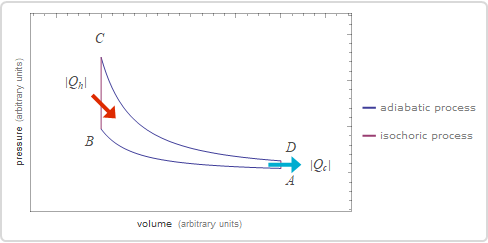
\includegraphics[width=\textwidth]{Figures/otto-cycle}
\decoRule

\caption[The Otto cycle]{The pV diagram of the thermodynamic Otto cycle. The
isochoric heat addition step (BC) corresponds to the burning of the homogeneous
air-fuel mixture. Work is extracted from the engine during the adiabatic
expansion CD \autocite{Wolfram|Alpha2019Otto}. }

\label{fig:otto-cycle}
\end{figure}

(These legs of the cycle are only loosely related to the `strokes' of a
four-stroke engine, and should not be confused for them.)

The theoretical efficiency of the Otto Cycle is given by 

\begin{equation}
	\eta = 1 - (\frac{1}{r^{\gamma-1}})
\label{eqn:otto-efficiency}
\end{equation}

where \(r\) is the \textit{compression ratio}, \( \frac{V_1}{V_2} \), and
\(\gamma\) is the heat capacity ratio, which can considered a constant for the
purposes of this discussion \autocite{Wolfram|Alpha2019Otto}.

This means that the efficiency of an Otto engine can be improved by increasing
the degree of compression of the intake air before combustion. 

\subsubsection{Diesel Cycle}

In the Diesel engine, named after Rudolf Diesel who demonstrated the first
engine of this type in 1897 \autocite[Chapter 14]{Cummins1989}, air is
compressed, and then a finely divided solid or liquid fuel is injected into the
system. The fuel then reacts with the oxygen in the air. The energy released in
the reaction appears as a higher temperature in the gas, and --- following
Gay-Lussac's Law --- the pressure of the gas rises. If the gases expands in the
confines of a collapsible vessel, useful work can be extracted from expansion of
the vessel. Once the work has been extracted, the vessel can be collapsed again
to remove the now inert ('exhausted') gas and prepare for receiving the next
charge of air, completing the cycle.

The theoretical cycle used to analyse the performance of the Diesel Engine is
called the Diesel Cycle. (See figure \ref{fig:diesel-cycle})

\begin{figure}
	\centering
	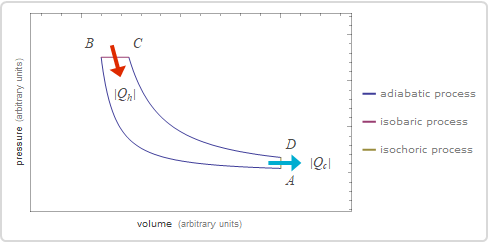
\includegraphics[width=\textwidth]{Figures/diesel-cycle}
	\decoRule

	\caption[The Diesel cycle]{The pV diagram of the thermodynamic Diesel cycle. The
	isobaric process BC corresponds to the combustion of the finely divided fuel
	particles in air. Work is extracted from the engine both during this process and
	during the adiabatic process CD. \autocite{Wolfram|Alpha2019Diesel}}

	\label{fig:diesel-cycle}
\end{figure}

The Diesel cycle differs from the Otto cycle in the heat addition step. In the
Otto engine, the heat addition takes place when the homogeneous air/fuel mixture
combusts. This combustion takes place in a short space of time during which
the engine parts move only a negligible distance. Hence the pressure rises
rapidly. In the Diesel engine, the fuel is injected into a volume of compressed
air, where it combusts. (There is no separate ignition source: the temperature
of the adiabatically compressed air is higher than the fuel's ignition
temperature, so that the fuel ignites upon injection. While this is another
difference between the two engines, it is of second-order importance when
discussing thermodynamic cycles.) Because the combustion takes place at the
surface of fuel particles, the combustion rate is lower than the combustion rate
of the homogeneous mixture in the Otto cycle. Hence the rising temperature is
balanced by the motion of the engine, and the heat addition is essentially
isobaric.

The efficiency of the Diesel cycle is given by Equation \ref{eqn:diesel-efficiency}

\begin{equation}
	\eta = 1 - \frac{1}{r^{(\gamma - 1 )}}(\frac{\alpha^{\gamma}-1}{\gamma(\alpha-1)})
\label{eqn:diesel-efficiency}
\end{equation}
 
where \(\alpha\) is the \textit{cut-off ratio} and \(\gamma\) is the compression ratio.

The term \( \frac{\alpha^{\gamma}-1}{\gamma(\alpha-1)} \) is always larger
than \(1 \), and therefore, when we compare equation \ref{eqn:diesel-efficiency}
with equation \ref{eqn:otto-efficiency} it is clear that for a given
compression ratio the Diesel cycle is always less thermally efficient than the
Otto cycle. 

However, at high compression ratios Otto engines start suffering from
`knocking', when the homogenous air/fuel mixture detonates, instead of burning
smoothly. The shock waves from this detonation will damage the engine and lead
to faster wear. (The \textit{octane number} of a fuel indicates the compression
ratio it can accommodate.) Because Diesel engines do not suffer from this
problem, they can, and usually are, designed to operate at higher compression
ratios than Otto engines.  Otto engines normally operate with a compression
ration of up to 9:1, where as Diesel engines have compression ratios of up to
25:1. This makes Diesel engines significantly more efficient than Otto engines. 

\subsubsection{Gas turbines and the Brayton Cycle}

The third internal\hyp{}combustion engine important to industrialized society is
the \textit{gas turbine}. Gas turbines are used rarely in road transport, more
often in marine and stationary applications, but thousands take to the sky
every day, propelling aircraft \autocite{Morris2017} carrying billions of airline
passengers every year.

The first gas turbines were developed during wartime urgency to deliver pure jet
thrust for military aircraft, but this proved to be an inefficient use of the
available energy. Most modern turbine engines drive a shaft to extract
rotational work. This shaft might drive a bypass fan (as used in airliner engines), a
propeller (as used in smaller, low-speed aircraft), or a shaft which might drive
a helicopter rotor or an electrical generator.

In operation, a gas turbine compresses air with one or more compressor stages.
The compressed air passes through a combustion chamber, where fuel is added and
combusted. As the now hot gases expand they pass through one or more turbine
stages, which is connected to drive the compressor and the output shaft, which
extracts work from the system. After the gas has passed through the turbine it
returns to atmospheric pressure, optionally doing work on the engine in the form
of thrust.

The theoretical thermodynamic cycle that is customarily used to analyse the gas
turbine is called the Brayton cycle, named after George Brayton, who
successfully manufactured a reciprocating engine based on this cycle. (See
figure \ref{fig:brayton-cycle}) Such engines are no longer
manufactured \autocite[Chapter 10]{Cummins1989}.

\begin{figure}
	\centering
	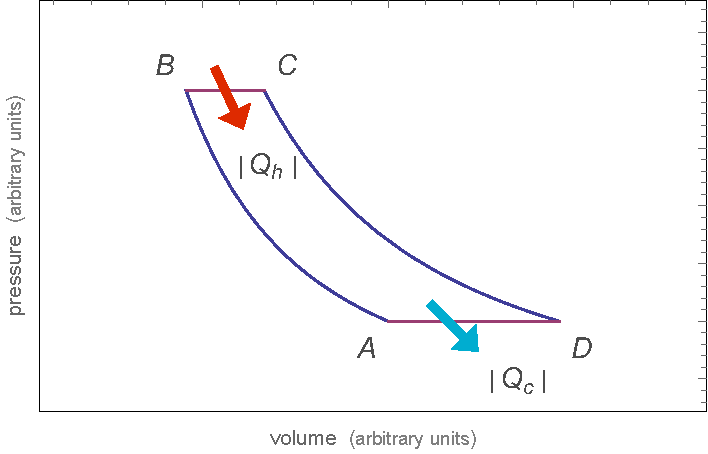
\includegraphics[width=\textwidth]{Figures/brayton-cycle}
	\decoRule
	
	\caption[The Brayton cycle]{The pV diagram of the thermodynamic Brayton cycle.
	In the gas turbine the continuous combustion of the injected fuel and free
	expansion of the air through a turbine means that the heat addition (BC) is
	isobaric. Work is extracted during the adiabatic expansion process CD
	\autocite{Wolfram|Alpha2019Brayton}.}
	
	\label{fig:brayton-cycle}
\end{figure}

The efficiency of the Brayton cycle is given by equation
\ref{eqn:brayton-efficiency} 

\begin{equation}
	\eta = 1 - \frac{T_{1}}{T_{2}} = 1 - (\frac{ P_{1} }{ P_{2} })^{(\frac{\gamma-1}{\gamma})}
\label{eqn:brayton-efficiency}
\end{equation}

where \(\gamma\) is the compression ratio \autocite{Wolfram|Alpha2019Brayton}.

Because the fuel is continuously added to the compressed air and the combustion
takes place in a heterogeneous mixture, gas turbines do not suffer from
`knocking' and therefore there is no upper limit to the compression ratio. The
main figure determining the efficiency of the engine is the turbine inlet
temperature, (\textit{i.e.} the outlet temperature of the combustion chamber)
which reaches 1600 °C in modern engines.

\subsection{Noxious pollution from internal combustion engines. }

Carbon pollution is not the only pollution emitted by internal combustion
engines. There is also noxious pollution, which affects the societies in which
they are used. There are ways to reduce or eliminate such pollution, but the
implementation of such measures affect the efficiency of the engine. 

Noxious pollution from internal\hyp{}combustion engines come from different sourc\-es
and have different effects.

\subsubsection{Unburnt fuel}

The combustion reactions in internal\hyp{}combustion engines are very fast, but
they are never at equilibrium. This means that at the end of a cycle, the
exhaust gases expelled from the engine contains, besides the carbon dioxide,
also chemical intermediates and unreacted fuel molecules.

Unreacted fuel is a noxious pollutant, not only in its own right, but also,
during the decomposition process in the environment, chemical reactions induced
by sunlight produces ozone, a reactive oxygen species that leads to respiratory
problems in victims of pollution \autocite{Davidson1998}.

Some of the fuel-like pollutants from internal\hyp{}combustion engines are not
present in the fuel. These compounds are formed in a process that might be
called \textit{pyro-synthesis}. They are themselves more stable than the
compounds from which they originate, but not as stable as the combustion end
products, carbon dioxide and water. Because they are themselves quite stable,
they require high temperatures to combust, which might not be achieved before
they leave the engine as waste. Notable pollutants from this source are the
policyclic aromatic hydrocarbons (PAH) and, if trace amounts of chlorinated
substances are present in the fuel, dioxins

One of the products of pyro-synthesis is particles of soot. These particles are
agglomerations of nano-sized particles of pure, amorphous carbon. The
agglomerations might include adsorbed PAHs and acids. Soot particles are very
stable and only react at very high temperatures. Diesel engines in particular
have a reputation for producing soot \autocite{Mohankumar2017}.

The final pollutant that can be classed as originating from partially combusted
fuel is carbon monoxide. It forms readily when fuels are burned in oxygen-poor
environments. Modern, well-maintained engines is a relatively rare cause of
acute carbon monoxide poisoning \autocite{Reumuth2018}, but chronic exposure to
low levels of environmental carbon monoxide has harmful effects
\autocite{Wright2002}.

\subsubsection{Contaminants and additives.}

Crude oil and coal contains not only carbon and hydrogen, but also other
elements, most notably sulfur and nitrogen. Depending on the refining process,
these elements might find their way into fuels. Organic nitrogen and sulfur will
easily oxidize and form stable oxides, yielding energy. Once outside the engine,
however, the volatile oxides will dissolve in any water in the air, forming
acids. \autocite{Duncan2016}

Fuel manufacturers add additives to fuels for various reasons, such boosting
octane rating or preventing corrosion. The prime example of additives as a
source of noxious pollution was tetraethyllead, which was added to petrol as an
octane booster. The emitted lead compounds was shown to be a pollutant that lead
to neurological impairment in its victims, and its use was phased out
\autocite{Needleman2000}.

\subsubsection{Side-reactions}

Most internal combustion engines use atmospheric air as oxidant. This air is
21\% oxygen, and 78\% nitrogen. Although nitrogen is very stable and inert, at
high temperatures it can react with oxygen. These reactions produce the oxides
of nitrogen: NO, NO$_2$, NO$_3$ and N$_2$O, and N$_2$O$_5$. They are
collectively called \nox.

These oxides can participate in the cycle that causes the photochemical smog.
They will also dissolve in atmospheric water and form acids: this might happen
far from the point of emission, resulting in \textit{acid rain}. 

\subsection{Mitigating pollution from internal\hyp{}combustion engines.}
 
Pollution from internal combustion engines is a social ill, and most governments
have regulations in place to limit and reduce this pollution. Engine and fuel
manufacturers are working hard to reduce this pollution.

The noxious pollution from internal combustion engines can be reduced by various
improvements, but there are three complementary approaches: fuel formulation
\autocite{Gertler1999}, cleanup \autocite{Braun2018} and engine management
\autocite{Reif2015}.

\subsubsection{Fuel formulation}

Adding oxygenates improves the octane rating of fuel and reduces \nox formation. 

\subsubsection{Exhaust gas cleanup} \label{par:cleanup}

Exhaust gases from internal combustion engines can be ``cleaned'', and there are
basically two approaches. The first is catalytic conversion, in which the
exhaust gases that contain the pollutants are passed over a catalyst bed. The
catalyst (a proprietary formulation of platinum, palladium and/or rhodium),
adsorbs the uncombusted volatile organic carbons, and oxidizes them. It
simultaneously catalytically decomposes \nox to molecular nitrogen and oxygen.

Secondly, filter systems can be used to remove particulate matter. 

\subsubsection{Engine management} \label{par:engine-management}

As described above, the main source of noxious pollution from
internal\hyp{}combustion engines is uncompleted or undesired chemical reactions,
and is not fundamental to the operation of the engine. By carefully managing the
engine system, noxious pollution can be reduced. 

The oldest engine management technology is the oxygen or `lambda' sensor, which
measures the oxygen in the exhaust gases. Such a sensor, coupled to an
engine-management computer, allows the me\-ter\-ing of the exact amount of fuel
need\-ed for op\-ti\-mum combustion \autocite{Frauhammer2014}.

A newer technology is known as exhaust gas recirculation. This mixes the intake
air of the engine with exhaust gases, effectively diluting the oxygen. This
reduces peak temperatures, and thereby \nox formation.

In \textit{stratified charge} engines the distribution of fuel in the volume of
intake air is controlled by selective fuel injection. Carefully injecting the
fuel at the right place at the right time can allow for higher compression
ratios without inducing pinging. \textit{Lean-burn} engines are Otto engines
that use use extremely high air:fuel ratios.

Electronic engine management systems result in much more efficient and
less-polluting engines than non-managed `mechanical' engines, but because
engines for automotive applications endure such a wide range of operating
conditions, they can at best achieve a compromise between power, efficiency and
emissions. It was this unsatisfactory compromise that lead to the Volkswagen
emissions scandal: manufacturers chose to cheat on emissions test rather than
admit to the relatively poor performance of a managed engine optimized for low
emissions \autocite{Mansouri2016}.

\subsubsection{Efficiency implications}

Attempts to mitigate noxious pollution from internal\hyp{}combustion engines
mostly lead to losses in efficiency. For example:

\begin{itemize}

\item Exhaust gas flow through catalytic converters and filters consume energy.
  
\item The engines cannot approach their theoretical maximum efficiencies,
because reducing \nox emissions is handled by limiting maximum combustion
temperatures.

\item \nox reduction catalysts require the presence of hydrocarbons,
\textit{i.e.} incomplete reactions, which implies that not all energy is
extracted from the fuel.

\item Every treatment system added to the engine adds weight to the vehicle, which
reduces payload and hence the total efficiency.

\end{itemize}

Before carbon dioxide pollution was a concern, it made sense to accept lower
efficiencies as a necessary cost of reducing noxious pollution, but in a
low-carbon future we cannot just keep on trading less noxious pollution for more
carbon dioxide production.

\subsection{Avoiding pollution from internal\hyp{}combustion engines} \label{par:carbon-neutral}

The efficiency and cleanness of internal\hyp{}combustion engines have
dramatically increased over the last century, and more improvements are being
implemented. But these improvements have not been fundamental to the engines in
any way, and have been driven mostly by government regulation, at the cost of
increased complexity and a higher purchase price.

It would seem obvious that it would be a good idea to introduce alternative
technologies. 

\subsubsection{Electrification}

In principle, there is nothing special about internal\hyp{}combustion engines:
they are not an end in themselves. They mere\-ly deliver a source of torque,
which can be coupled to machinery to do useful work. Before the industrial era
such torque was available from windmills and waterwheels, and today an
alternative is the electric motor.

Electric motors are engines that use the interaction between electric current
and magnetic fields to deliver useful torque to drive machines. Because they use
electricity as a source of energy, they have no noxious emissions where they
operate. Because they are not heat engines, their efficiencies are not subject
to the Carnot limit, and efficiencies exceeding 95\% are standard \autocite{Li2012}.

Electricity, of course, is not necessarily carbon-neutral. Most electricity is
generated in power plants that use fossil fuels as a primary source of energy.
But because these plants are huge, and efficiency scales disproportionately with
size, the energy output by the electric motor has a similar or lower carbon
footprint than an equivalent internal\hyp{}combustion engine \autocite{Doucette2011}.

Electricity grids are also increasingly being fed by solar and wind power,
which are carbon-neutral at source. These renewable plants are also smaller and
more flexible than their behemoth fossil-fuel counterparts, with lower capital
costs and extremely low running costs.

Hence, in a low-carbon future, there is every reason to support or mandate the
use of electrical motors for stationary applications wherever possible.

In automotive applications, \textit{i.e.} in cases where the engine is used to
move itself in addition to some form of payload, the application of electric
motors is more demanding. In this case it is not easy to bring the electricity
to the motor, although electric trains and buses fed by overhead conductors are
splendid examples of the electrification of transport. So for electric vehicles
to use the existing road network, they need to carry a source of electricity
with them.

This source of electricity can be a either a chemical battery, or a fuel cell.
In a chemical battery power from the grid is stored in the form of reversible
electrochemical reaction, and in a fuel cell the chemical energy from a fuel is
directly converted into electricity. There are fuel cells that can use hydrogen
as a fuel, and fuel cells that can use methanol as a fuel. (It goes without
saying that the hydrogen and the methanol need to be sourced from low-carbon
sources for fuel cells to count as low-carbon energy sources.)

The storage and transport of hydrogen remain hurdles to the large-scale adoption
of hydrogen-fuelled automobiles, although a market seems to be developing for
hydrogen-fuelled electric trains \autocite{theguardian_2018}. Hydrogen fuel cells
emit no carbon or noxious pollution at point of use.

Direct methanol fuel cells can react methanol with atmospheric oxygen in an
electrochemical cell to yield electricity, with carbon dioxide
as a waste product. Little is known about possible noxious pollution.

At this time it seems that the electrification of road transport will be by
chemical batteries. Lithium-ion batteries can now store enough energy and
deliver enough power to make electric motor vehicles practical and
attractive \autocite{Hayes2011}, and some governments are considering plans to no
longer allow the production of passenger vehicles propelled by internal
combustion engines \autocite{Burke-Kennedy2018} \autocite{Reuters2018}
\autocite{Gabbatiss2018}.

\subsubsection{Carbon-neutral fuels} 

Another way to avoid the carbon pollution associated with internal-combustion
engines is to change the fuel. Not all fuels are fossil fuels, and it is
possible to use fuels that are carbon neutral, and in some cases carbon
negative.

Apart from using hydrogen in a fuel cell, as described above, \textit{hydrogen}
can also be used as a fuel in Otto engines, because it will combust in air to
yield heat. The emissions are water and \nox. Presently there are no
hydrogen-fuelled Otto engines on the market.

Methanol is a common product of the fossil fuel industry, but work is underway
to produce methanol by reducing carbon dioxide using solar energy. Such
\textit{solar methanol} might be used in direct conversion fuel cells, or in
internal\hyp{}combustion engines.

It is possible to harness the energy in contained in the reduced carbon in
biological materials and use it as fuel. Such fuels are known as
\textit{biofuels}.

\section{Biofuels}

Biological processes are an integral part of the carbon cycle, because
photosynthesis in plants reduces carbon dioxide in the atmosphere to sugars,
which are converted by plant physiology into structural cellulose and other
metabolites.

The prototypical biofuel is of course wood, used in all societies for cooking
and heating. This familiarity makes biofuels seem an obvious and viable
source of energy, but details matter, and switching from fossil fuels to
biofuels to reduce carbon footprints of human activities is not a simple choice.

Firstly, the efficiency of photosynthesis is notoriously low: not above a few
per cent, whereas the efficiency of a mass-produced silicon-based solar panel is
in excess of 20\%. In general it is much more efficient to capture solar energy
in a PV panel and use an electric motor to provide the necessary mechanical
power than to create a biofuel and use it to drive an internal-combustion
engine.
 
Second, increased biofuel production has numerous impacts on the environment and
society, which cannot be ignored.

Discussing all the factors that need to be studied to make such a decision is
outside the scope of this work, but as an example a report prepared for
stakeholders in the Netherlands \autocite{Smeets2006} uses the following criteria:

\begin{itemize}
  \item GHG [greenhouse gas] emissions – the use of biofuels should cause reductions of GHG emissions. The
comparison should be done regarding the average use of fossil fuels, considering the life
cycle of fossil and biofuels (\text{i.e.}, well-to-wheel basis) and in case of biofuels reduction
should be at least 30\%
 \item Impacts over food supply – the production of biomass for energy must not endanger the
food supply and other local biomass applications. The analysis should be developed
considering possible changes of land use in the region of biomass production.
 \item Biodiversity – Biomass production must not affect protected or vulnerable biodiversity.
 \item The basic criteria are that violation of national laws and regulations are unacceptable.
 \item Local environmental effects – Principles include (a) soil and soil quality, that must be
retained or even improved, (b) ground and surface water supply, that must not be polluted.
 \item Local economic effects – The production of biomass must contribute towards local
prosperity.
 \item  Social well-being – The production of biomass must not decrease the well-being of local societies. 
\end{itemize}

Nevertheless, there are cases where using biofuels is a good option. 

\subsection{Bio-gas}

Anaerobic bacteria can convert biogenic carbon compounds to methane. This
methane is identical to the methane obtained from natural gas, and can be used
for the same applications.

An excellent application for the use of bio-gas is waste remediation. Waste
material from the agri-food industry can be highly polluting if not treated
properly, emitting noxious chemicals into water and the potent greenhouse gas
methane into the atmosphere. But when used as feedstock for bio-gas production,
it reduces carbon pollution by capturing methane and displacing natural gas, and
also prevents water pollution \autocite{Venter2014}. 

Bio-gas can be used to fuel Otto engines or gas turbines. 

\subsection{Bio-ethanol}
\label{sec:BioEthanol}
Yeast and other microbes can convert sugar or starch from plants into ethanol.
This technology is as old as civilization. Archaeologists may be in disagreement
where beer was brewed first, but it is clear that between 3200 and 3000 BCE in
ancient Sumeria the brewing of beer was an activity regulated by the government
\autocite{Damerow2012}. By 2000 BCE in ancient Egypt the technology of
fermentation was harnessed well enough that bakeries and breweries were
co-located \autocite{1920}.

Beer and wine can best be described chemically as aqueous solutions of sugars,
ethanol, flavourants and colourants, with or without suspended solids. It was
not until the 8th century CE that Persian and Arab scientists mastered the art
of distillation and purified ethanol \autocite{Modanlou2008}, and it was not
until Pasteur that yeast was seen as a living organism, and ethanol a product of
its metabolism \autocite{Barnett2000}.

It is unclear when ethanol was firsted as a fuel, but its flammability must have
been noticed by the first distillers. By 1838 ethanol was common enough to be
used in alcohol lamps as a source of heat in the chemical laboratory
\autocite{Griffin1838}, and by the 1850s it was a major component of lamp oil
used for illumination in the USA \autocite{Abebe2008}.

Ethanol as a fuel for internal combustion engines has a clear start date: in 1826
Samuel Morley was granted a patent for an engine designed to use ethanol as fuel
\autocite[p. 79]{Cummins1989}.

The industrial production of ethanol is a technologically advanced process. It
is an active research field. A paper \autocite{Cardona2007} reviewing the process
technology of producing bio-ethanol written in 2007 had garnered 644 citations
by January 2019.

The industrial production of ethanol consists of three steps. 

\begin{enumerate}
  \item Fermentation
  \item Distillation
  \item Dehydration
\end{enumerate} 

The fermentation step is the biological process by which the yeast organism
\textit{Saccharomyces cerevisiae} convert the sugar and starch in the biological
material to ethanol and carbon dioxide. This needs to be done in a sterile
environment to prevent contamination by other micro-organism.

The distillation step is the physical process of separating the produced alcohol
from the aqueous mixture in which it is produced. This generally produces an
azeotropic mixture that contains 95.6 \% ethanol \autocite{Kumar2010}.

While the processes of fermentation and distillation of ethanol for fuel is in
principle the same as that of producing alcoholic beverages, the emphasis of the
processes are very different. In the beverage industry the emphasis is on the
development of complex flavours and a consistent, recognizable drinking 
experience. In the fuel industry the emphasis is on efficiency and throughput.

To produce fuel-grade ethanol from the distilled azeotrope, dehydration is a
necessary third step. This step can be implemented by various distillation
processes that add a third compound, but in most modern plants the water is
removed by adsorption onto molecular sieves \autocite{Kumar2010}.

\subsubsection{Brazilian ethanol}

Brazilian sugar-cane ethanol is an integral part of the country's energy
network. Most Otto-engine vehicles have `flex-fuel' engines, which can be
fuelled with any blend of ethanol and petrol. The industry is regarded as
sustainable (\autocite{Smeets2006}.

\subsubsection{US maize}

US maize ethanol is primarily blended with petrol to meet legislative
requirements of oxygenates in fuels. The production of maize is water-intensive
and the fermentation process is carbon-intensive. The US ethanol from maize has
a poorer energy balance and larger carbon footprint than Brazilian ethanol from
sugar cane, but has a smaller water footprint \autocite{Mekonnen2018}.

Ethanol can fuel Otto engines and gas turbines. 

\subsection{Fischer-Tropsch fuel from biomass}
\label{sec:FT}

It is possible to heat woody biomass with steam in a low-oxygen environment to
produce synthesis gas, which can be the converted to a mix of fuel products in
the well-known Fischer-Tropsch catalytic process. Such a  fuel could be called a
bio-fuel, but it's production would be difficult to reconcile with the
principles of \textit{green chemistry}, described in Section
\ref{sec:GreenChemistry}.

\subsection{Hydrotreated vegetable oil: ``Green diesel''}
\label{sec:GreenDiesel}

The petroleum industry has developed a collection of chemical processes, such as
hydrogenation, oxygenation and cracking. This collection of processes can be
applied to vegetable oils to produce a fuel for diesel engines and gas turbines.
This path is being followed by the aviation industry \autocite{Chiaramonti2014}.

\subsection{Biodiesel}

Oils and fats have been used as fuels since antiquity, most obviously as a fuel
for lamps: olive oil has been identified as the fuel used in lamps dating from
around 600 CE \autocite{Kimpe2001}, and at the Paris World Fair in 1900 Rudolf
Diesel demonstrated an engine that ran on peanut oil \autocite{Knothe2010}.

During the energy crisis of the 1970s, the South African government looked at
alternative sources of fuel. Experiments were done with sunflower oil in
tractors, but there was a problem with the formation of carbon deposits around
the injector nozzles. Seeing that the clogging of the injectors might be caused
by the high viscosity of the sunflower oil as a fuel, the transesterification of
the oil was implemented, replacing the glycerol in the sunflower oil with
methanol. This created an oily liquid with a lower viscosity, which proved to be
a trouble-free replacement \autocite{VanNiekerk1980}.

Such a transformed oil is termed \textit{biodiesel}. It consists primarily of a
mixture of fatty acid methyl esters, often abbreviated into the acronym FAMEs.

Compared to ethanol, biodiesel production is relatively simple, the main method
sharing much with the ancient technology of making soap. This simplicity makes
the production of biodiesel attractive to small and decentralized manufacturing,
and consequently governments consider biodiesel production an attractive
proposition: it can create job opportunities in rural population and it can
create a stable market for farmers who produce vegetable oil crops.

\begin{figure}
	\centering
	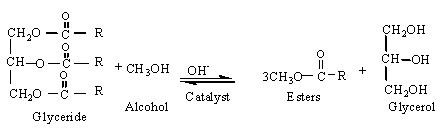
\includegraphics[width=\textwidth]{Figures/reaction}
	\decoRule
	\caption[Transesterification]{Transesterification}
	\label{fig:Electron}
\end{figure}

Biodiesel is not yet carbon neutral: the methanol used to create the methyl
esters is a product of the petroleum industry, and therefore biodiesel emissions
contribute to global warming. But replacing fossil diesel fuel with biodiesel
results in a nett reduction of carbon emissions, with the future possibility of
replacing fossil-derived methanol with carbon-neutral bio-methanol
\autocite{Shamsul2014}.

% ----------------------------------------------------------------------------------------
% SECTION 4
% --------------------------------
\section{The significance of biodiesel and its quality control.}

In a complex technical, economic and social environment it is likely that there
will always be a need that can be best met by internal combustion engines. The
decision on the type of engine and the decision on the fuel for that engine are
not independent, as Cummins reminds us \autocite{Cummins1989}:

\begin{quotation}
``Our generation faces a similar challenge in a real liquid fuel energy shortage
that will come within the lifetime now living. As we plunge into the seeking of
solutions to our dilemma, we must never forget that \textit{an engine and the
fuel it consumes are inseparable partners}; the one cannot progress without the
full cooperation of the other. This precept is vital to the planning of future
powerplants, since an engine's design determines its fuel and binds us to our
future resource requirements.''
\end{quotation}

While the variation-selection process by which real engineering progress is
`blind', \textit{i.e.} the combination of factors that make a design successful
is not known at the start of a development \autocite{Vincenti1990}, scientific
knowledge provides guidance in the form of insight into processes and
theoretically achievable targets for performance. Using the scientific knowledge
we have today, we can  risk a forecast: if society is determined that its carbon
footprint should be reduced with minimal noxious pollution the application of
internal combustion engines would tend towards the following:

\begin{enumerate}
  
  \item Larger: Because larger engines are more efficient than smaller engines,
  larger engines will be preferred. (See section \ref{par:scaling})
  
  \item Low-carbon: The preferred engine would be fuelled by carbon-neutral
  fuels. (Section \ref{par:carbon-neutral})
  
  \item Constant speed: Engines are most efficient when they can work at
  constant load. (Section \ref{par:engine-management})
  
  \item Efficient: Engines with high efficiency should be preferred, which
  implies engines with high compression or pressure ratios. (Section
  \ref{par:efficiency})
  
  \item Cleanup: The exhaust should be amenable to cleanup, \textit{i.e.} the
  exhaust gases of the fuel-engine system should not contain compounds that are
  incompatible with available converter or filter technologies. (Section
  \ref{par:cleanup})
     
\end{enumerate} 

From this it should be clear that the optimal engine of the future will not be
an Otto engine, because it will always have a limited compression ratio and its
catalytic exhaust cleanup will always require stoichiometric air:fuel ratios,
which puts bounds to efficiency increases.

Because it is the most efficient engine, the gas turbine will play an important
role. However, its exhaust temperature is very high, which begs for energy
recovery to increase the efficiency of the system. Such systems are already seen
in the \textit{combined cycle gas turbine} (CCGT). But energy recovery systems
are not light and small, so their best application outside aerospace (where the
excess heat is utilized as thrust) appears to be stationary electricity
generation.

For automotive applications the engine that will best contribute to reduce the
carbon footprint of may be a large Diesel engine with exhaust cleanup to remove
\nox and soot, fuelled with a carbon-neutral fuel.

In choosing between refined vegetable oil and biodiesel as a fuel, it is most
likely that biodiesel will have a lower carbon footprint. Refinery operations
are energy intensive, which might add to the carbon footprint of the fuel, and
refineries are not usually near the point of use, so that transport will also
add to its carbon footprint. The carbon emissions of biodiesel production are
comparatively low. (At this point it is important to note that these
observations are not definitive: carbon footprints are not predicted, they must
be calculated.)

Buying large, highly efficient diesel engines with sophisticated management
systems and exhaust cleanup require high capital investment. In an economically
competitive environment they therefore need to bring reliable returns, which
implies high availability, as measured by frequency of breakdown and length of
time between maintenance stops. Such high reliability can only be achieved if
the manufacturer understands the fuel-engine system well and it behaves
predictably.

In a low-carbon future, therefore, well-characterized biodiesel might be
expected to play a central role in non-electric ground transport and industrial
application where electrification is not possible.

\section{Conclusion: the role of chromatography.}

The development of the fuel-engine systems depends heavily on the chemical
characterization of fuels and engine emissions, and chromatography has always
played a central role: some of the earliest researchers developing gas
chromatography were employees of a petrochemical company
\autocite{Keulemans1955}.

This thesis explores the possibility of applying comprehensive two-dimensional
(supercritical fluid $\times$ gas) chromatography to the chemical
analysis of biodiesel for the purpose of characterization and quality control. 

% ----------------------------------------------------------------------------------------
% SECTION 5
% --------------------------------


% Chapter 2

\begin{savequote}[\quotewidth]
$PV \ne nRT$
\qauthor{The ideal gas law does not apply to supercritical fluids.}
\end{savequote}

\chapter{Introduction: Carbon dioxide and chromatography} % Main chapter title

\label{Chapter2} % Change X to a consecutive number; for referencing this chapter elsewhere, use \ref{ChapterX}


%----------------------------------------------------------------------------------------
%	SECTION 1
%----------------------------------------------------------------------------------------

\section{The chemical industry}

Industrialized societies depend on chemicals. (In this discussion I define
chemicals as pure substances that are produced by industry for industry.)
Chemicals might be used in the processing of products, or blended with other
chemicals in formulations that might be sold to users as products. In a familiar
example, sugar is a chemical produced by the sugar industry from sugar cane or sugar beet.
It is a pure substance (sucrose) that is mostly used in the industry as an
ingredient for processed food. Other uses of sugar include coatings for
medication, and feedstock for engineered micro-organisms that produce pharmaceuticals. (Sugar is a
rare example of a chemical that is also sold to consumers.)
 
The chemical industry produces a huge variety of products, from compounds as as
simple as hydrochloric acid to compound as sophisticated as cyanocobalamin
(Figure \ref{fig:vitb12}). All of these chemicals help produce the products
indispensable to industrialized societies. Nevertheless, the chemical industry
is not held in high regard by people outside the industry. A part of this
negative perception comes from the chemical industry's reputation for fatal
accidents and pollution \autocite{Gumm2015}.

\begin{figure}
\centering
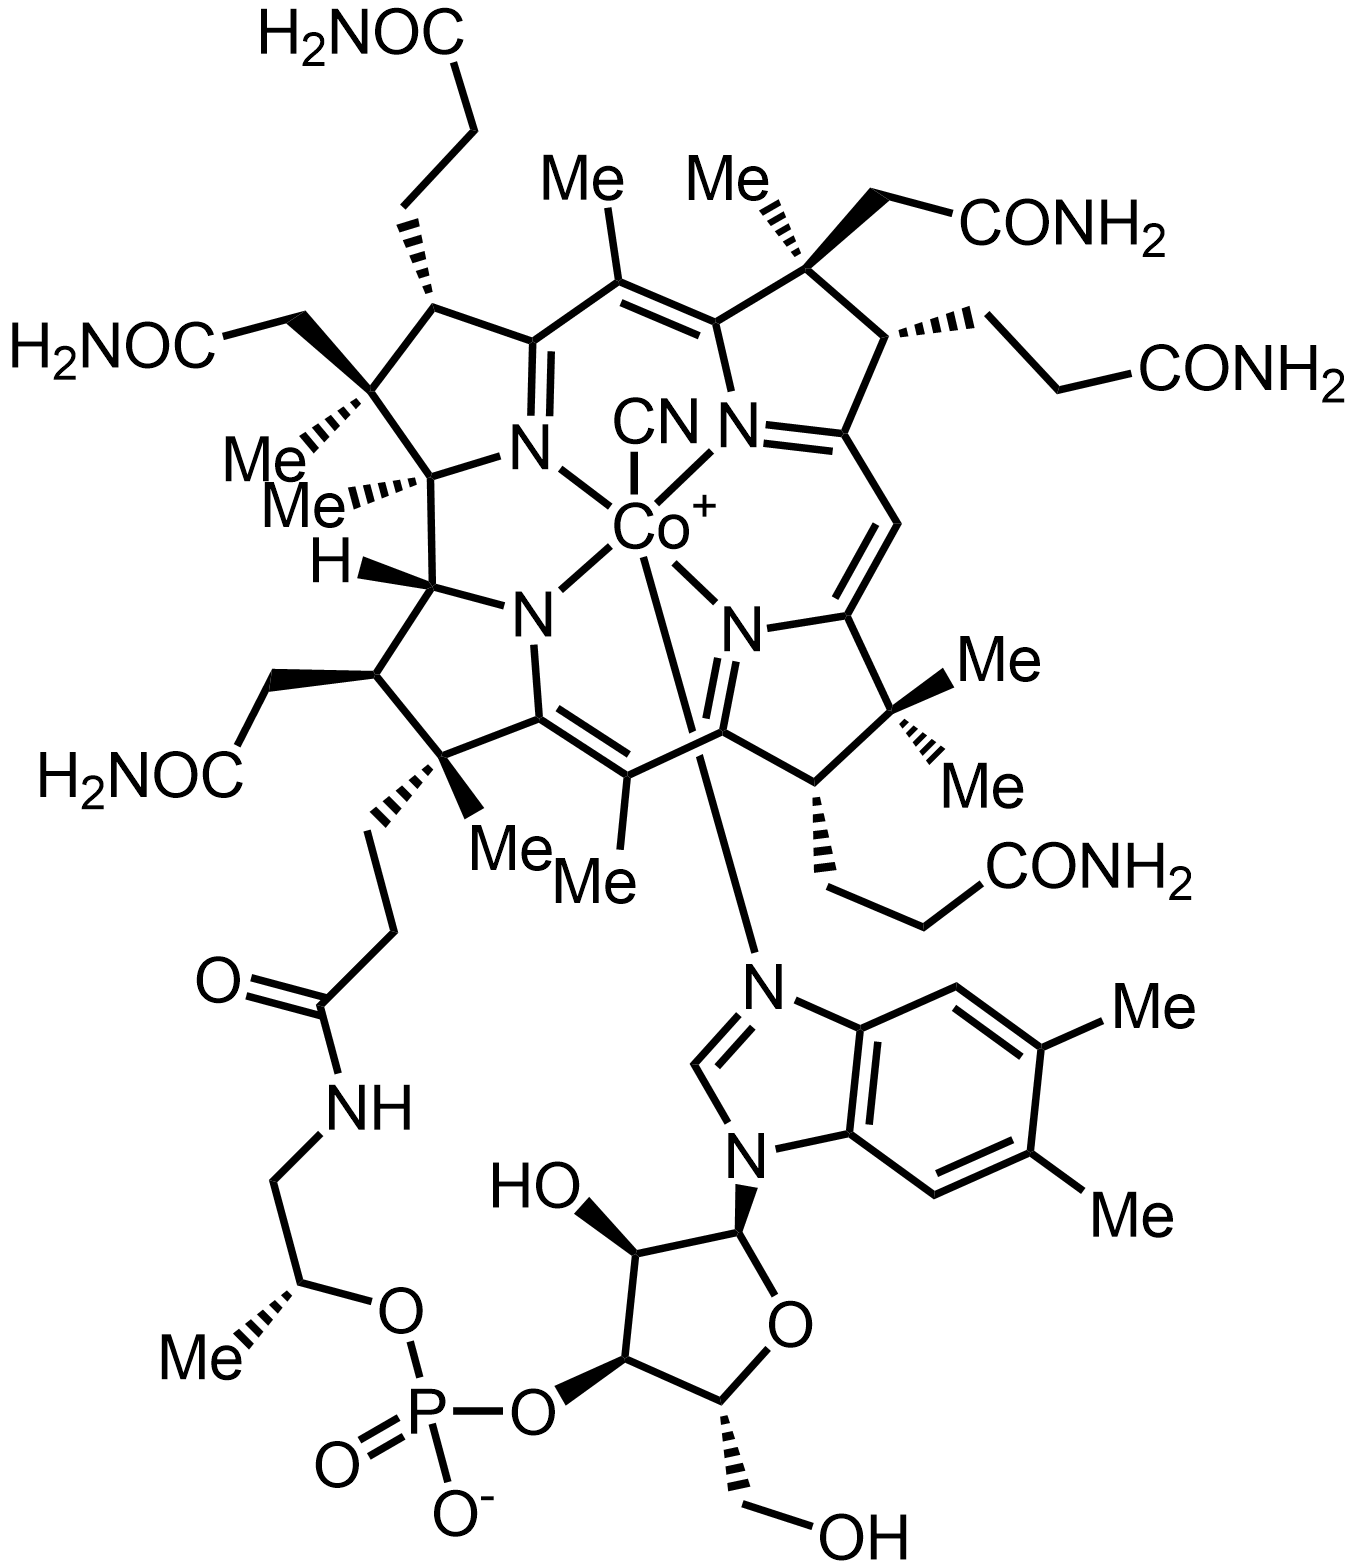
\includegraphics[width=\textwidth]{Figures/Cyanocobalamin-b12.png}
\decoRule
\caption[Cyanocobalamin]{The chemical structure of cyanocobalamin, a form of vitamin B12. This compound is produced on the tonne scale by the chemical industry.}
\label{fig:vitb12}
\end{figure}

The list of incidents is long and examples easily spring to mind: In 1984 a leak
at a chemical plant in Bhopal, India, caused the death of thousands of people
and the injury of thousands more \autocite{Varma2005}.
Stratospheric ozone is struggling to recover from depletion caused by the
reckless emissions of chlorofluorocarbons \autocite{Ball2018}. Plastics
microparticles are now found everywhere in the oceans \autocite{Woodall2014},
and the pesticide DDT is found in the breast milk of Inuit mothers
\autocite{Gibson2016}.

The chemical industry is also a prodigious producer of greenhouse gases. Apart
from the carbon dioxide emitted by the production of the energy that power
chemical processes, some chemical processes emit carbon dioxide as a waste
product. Most notable of these is the reduction of atmospheric nitrogen as the
first step in the production of nitrogen fertilizers. Of all the greenhouse
gases monitored by the IPCC, only carbon dioxide, methane and nitrous oxide are
found in nature: the others are exclusively products of the chemical industry
\autocite{IPCC2014}.

No chemical has ever jumped out of a lab, multiplied uncontrollably, and spread
into the environment to poison or pollute: they have all been introduced into
the environment by human ignorance, negligence, or recklessness. All chemicals
behave well when used in properly controlled environments, but human actions can
let them escape and damage and pollute. But while we try to solve the
intractable problem of human behaviour, we as chemists cannot just lay blame: we
must pay attention to the intrinsic safety of chemicals and chemical processes.
 
%-----------------------------------
%	SUBSECTION 1
%-----------------------------------
\subsection{``Green chemistry''}
\label{sec:GreenChemistry}
The date of the birth environmental movement is conventionally set to 1962, when
the biologist Rachel Carson published the book \textit{Silent Spring}, which
pointed out the destruction of nature by the unrestricted use of pesticides, and
the dangers of overuse \autocite{Carson1962}. This was a direct imputation of
the chemical industry, because the pesticide products contained many chemicals.

Chemists are human, and the realization uncontrolled that chemicals can have
detrimental effects lead at least some chemists to reflect on their own work.
This has given rise to the concept of \keyword{green chemistry}. Although the
term has no rigorous definition or quantitative measure \autocite{Linthorst2010},
a set of 12 principles or guidelines are proposed:

\begin{enumerate}
  \item \label{itm:waste}It is better to prevent waste than to treat or clean up waste after it is formed.
  
  \item \label{itm:incorporation}Synthetic methods should be designed to maximize the incorporation of
  all materials used in the process into the final product.
  
  \item \label{itm:toxicity}Wherever practicable, synthetic methodologies should be designed to use
  and generate substances that possess little or no toxicity to human health and
  the environment.
  
  \item \label{itm:efficacy}Chemical products should be designed to preserve efficacy of function
  while reducing toxicity.
  
  \item \label{itm:aux}The use of auxiliary substances (\textit{e.g.} solvents, separation agents, etc.)
  should be made unnecessary wherever possible and innocuous when used.
  
  \item \label{itm:energy}Energy requirements should be recognized for their environmental and
  economic impacts and should be minimized. Synthetic methods should be
  conducted at ambient temperature and pressure.
  
  \item \label{itm:renewable}A raw material or feedstock should be renewable
  rather than depleting wherever technically and economically practicable.
  
  \item \label{itm:derivatization}Unnecessary derivatization (blocking group, protection/deprotection,
  temporary modification of physical/chemical processes) should be avoided
  whenever possible.
  
  \item \label{itm:catalysts}Catalytic reagents (as selective as possible) are superior to
  stoichiometric reagents.
  
  \item \label{itm:persistence}Chemical products should be designed so that at the end of their
  function they do not persist in the environment and break down into innocuous
  degradation products.
  
  \item \label{itm:monitoring}Analytical methodologies need to be further developed to allow for
  real-time, in process monitoring and control prior to the formation of
  hazardous substances.
  
  \item \label{itm:safe}Substances and the form of a substance used in a chemical process should
  be chosen so as to minimize the potential for chemical accidents, including
  releases, explosions, and fires.

\end{enumerate}

While these guidelines are clearly written with synthetic chemistry in mind, it
does not mean that they do not apply to analytical chemistry. For example,
Principle \ref{itm:renewable} suggests that, when possible, one should use
hydrogen rather than helium as mobile phase in capillary gas chromatography:
hydrogen is renewable, whereas helium is a finite resource and from time-to-time
there are reports of shortages \autocite{Kornblut2019}.

One large area of the greening of chemistry is changing the use of solvents.
Principle \ref{itm:aux} recommends that solvents use be avoided, if possible ---
most solvents used in chemistry are ultimately derived from petroleum and are
toxic to some degree. But solvents play a large role in many kinds of chemistry,
and eliminating their use in the near future seems unlikely. Searching for and
characterizing bio-derived, non-toxic, non-persistent solvents is an active
field of research \autocite{Clarke2018}.

%%One application for solvents is extractions. Extractions can be either from a
%%solid material, as in extracting aspirin from willow bark, or liquid-liquid,
%%where a compound is extracted from one liquid into another. Liquid-liquid
%%extractions might be used to extract fragrance compounds from essential oils,
%%%for example.

But there are a few solvents in already current use that are inherently
``green'', such as water or ethanol.

One such naturally green solvent is carbon dioxide. 
 
% ----------------------------------- SUBSECTION 2
% -----------------------------------

\subsection{Carbon dioxide as a green chemical}

Carbon dioxide as a chemical is used in industry in a few key areas.

\begin{itemize}
  
  \item Carbon dioxide is often used in firefighting, in the form of portable
  fire extinguishers or room flooding systems. In this last use it is
  displacing the ozone-depleting halomethane (Halon).
  
  \item When liquid water is supersaturated with carbon dioxide, the gas
  desolvates slowly in the form of streams of tiny bubbles. This phenomenon
  makes beverages prepared from water supersaturated with carbon dioxide (or
  \keyword{carbonated water}) interesting to drink, and a large, international
  beverage industry is based on carbonated water.
   
   \item Carbon dioxide has a freezing point of {-}77 °C, and the solid can be
   conveniently obtained by evaporating liquid carbon dioxide at atmospheric
   pressure. The evaporating liquid rapidly cools the stream of carbon dioxide,
   lowering the temperature of the stream to below the freezing point, and the
   gas crystallizes into the solid. The resulting `snow' can be compressed into
   blocks, which only slowly sublimates into gaseous carbon dioxide, keeping the
   temperature at the freezing point. Packing frozen food products together with
   this 'dry ice' allows for it to be transported cold.
   
   \item Pellets of dry ice can be entrained in a jet of air, and used to abrade
   surfaces for cleaning \autocite{Spur1999}. This use of carbon dioxide can
   displace toxic solvents or abate the noxious dust produced by blasting operations.
   
   \item Carbon dioxide is a `natural refrigerant' \autocite{Pearson2005}, and
   can be used to displace hydrofluorocarbon refrigerants, which are potent,
   long-lived greenhouse gases.
   
   \item Carbon dioxide can be used as a preservative and anti-oxidant in
   packaged food. If air in a packaged food is removed by purging the headspace
   with carbon dioxide, the growth of microbes can be discouraged, extending the
   shelf life of the product \autocite{Jacobsen2002}.
	   
	\item Carbon dioxide can be used to extract compounds from natural products. 
	
\end{itemize}

Of these uses, extractions are economically the most important.

\section{Extractions using carbon dioxide}

\subsection{Commercial extractions}

There are several commercial processes that use carbon dioxide to extract
valuable products from plant material.

\subsubsection{Plant oils}

Vegetable oils are obtained from various crops, and can be extracted from the
plant material by pressing, heating or extraction. High-pressure carbon dioxide
has been used to extract vegetable oils from various plants, although it seems
that this process has only found niche applications so far
\autocite{Eisenmenger2006,Grazyna2018}.

\subsubsection{Hops}

Hops is an essential component in the brewing of beer. It imparts a desired
bitter flavour, stabilizes the beer during storage, and assists with foam
formation \autocite{Schoenberger2011}. Hops is a seasonal crop with a limited
growing range, but the demand for beer is not limited to certain areas or
seasons. The creation of hops extract makes it possible for brewers to benefit from 
hops without owning a hops plantation or storing and transporting dried hops
over long distances. All hops extracts produced today are extracted by carbon
dioxide \autocite{Hunt2010}.

\subsubsection{Coffee}

Coffee is an international industry, with coffee drunk in many cultures and in
many forms. One of the attractions of coffee is the effects of the psychoactive
substance found in the coffee bean, \keyword{caffeine}. Caffeine is a mild
stimulant and promotes wakefulness. A small proportion of coffee drinkers enjoy
drinking coffee, but prefer to avoid the stimulant effect, which might induce
insomnia or irritability. For these coffee drinkers the market supplies
\keyword{decaffeinated coffee}.

Given the large amount of coffee traded (an estimated 167.47 million bags of
coffee in the 2018-2019 coffee year \autocite{Coffee2018})\footnote{The factoid
that ``coffee is the second-most traded commodity after oil'' has been proven to
be untrue \autocite{Greenberg2017}.}, if only a small percentage of coffee needs
to be decaffeinated, it will be a large amount of coffee to process, and
industrial processes will be necessary to supply the demand.

Decaffeination of coffee is achieved by selectively extracting the caffeine from
green (\textit{i.e.} unroasted) coffee beans using carbon dioxide. This is the
largest use of carbon dioxide for extraction \autocite{Ramalakshmi1999}. The
extracted caffeine is sold for use in medication and `energy' drinks. 

\subsection{Analytical Extractions}

Extraction is not only an industrial process, but is part and parcel of analytical
chemistry. The first extractions using carbon dioxide was not aimed at developing
an industrial operation, but to develop methods for analytical chemistry. This
method is usually called SFE, for \textbf{s}upercritical \textbf{f}luid
\textbf{e}xtraction.

\subsection{Why carbon dioxde?}

But what makes carbon dioxide a suitable solvent for extraction?

There are two aspect to this question. The first is about the \textit{greenness}
of carbon dioxide. It is non-toxic, non-persistent, non-flammable,
non-corrosive, inexpensive, commercially available, and a waste product. (It
goes without saying that this carbon dioxide is sourced from a carbon-neutral
source, perhaps the brewing industry.) The second aspect of the desirability of
carbon dioxide lies in its physical properties and the conditions under which we
use it.

Chemists will intuitively understand that gaseous carbon dioxide has no solvating
properties, and that liquid carbon dioxide should not behave much differently
than any other solvent. Both these statements are true under `normal' circumstances.

But consider the case of an isobaric cooling of a volume of gas. The gas-liquid
transition takes place because energy is removed from the system. At some point
the kinetic energy of some of the molecules becomes less than the energy of the
intermolecular forces, and the molecules prefer to clump together, \textit{i.e.}
it condenses. The remaining gas molecules receive the excess energy, and
therefore stay in the gas state, until more energy is removed, leading to more
of the gas condensing. During this process the temperature remains constant, and
this temperature is known as the boiling point.

Now consider a solute (solid or liquid) in the same volume of gas being cooled.
In this case, as the gas cools, the gas-solute intermolecular forces can become
stronger than than the gas-gas intermolecular forces at a temperature which is
higher than the boiling point. In such a case the gas molecules will clump
around solute molecules, while the kinetic energy of the gas molecules are still
too high to allow condensation. Now the gas has obtained solvating properties
and the solute will become truly dissolved in the gas.

The same effect can be imagined to happen during the isothermal compression of a
gas.

If there are more than one solute in the volume of gas, some might dissolve in
the gas, while others one might not. This means that the solvating gas can be
\keyword{selective}. It can also be seen that the solvating power of the gas will
depend on the temperature and the pressure of the gas. This means that the
solvent becomes \keyword{tunable}.

While the dense gas has solvating properties, it still has the physical
properties of a gas:

\begin{description} 

\item[Diffusivity] The solvating gas maintains its low diffusion coefficients,
which means that it can easily diffuse into porous material, and that solutes
will rapidly diffuse through it.

\item[Surface tension] The solvating gas has a low surface tension, which means
that it will readily `wet' surfaces and penetrate porous material.

\item[Viscosity] The solvating gas has a low viscosity, which means that it
takes little energy to pump it.

\end{description} 

For historical reasons such solvating gases are known as a 'supercritical
fluids', because they were first obtained by heating a liquid at high pressure
\autocite{Berche2009}, so that the temperature and pressure of the substance is
higher than it's \keyword{critical point}. The critical pressure of a substance
is the pressure above which it is impossible to create a gas-liquid phase
transition by isobaric cooling, and the critical temperature is the temperature
above which it is impossible to create a gas-liquid phase transition by
isothermal compression.
When the gas is at its critical temperature and critical pressure, it is at its
critical point. The critical point is very different from the \keyword{triple
point}: there is no equilibrium involved (See figure \ref{fig:co2phase}). The
terms `supercritical fluid' and `dense gas' are synonyms \autocite{Randall1982}
--- the adjective `dense' in `dense gas' of course implies that the gas
behaviour is far from that of an ideal gas.

There are no discontinuities in binary diffusivity when temperature is changed
from above to below the critical temperature \autocite{Lauer1983}. Hence
extractions are often done under conditions which are not technically
'supercritical' but still yields its benefits.


\begin{figure}
\centering
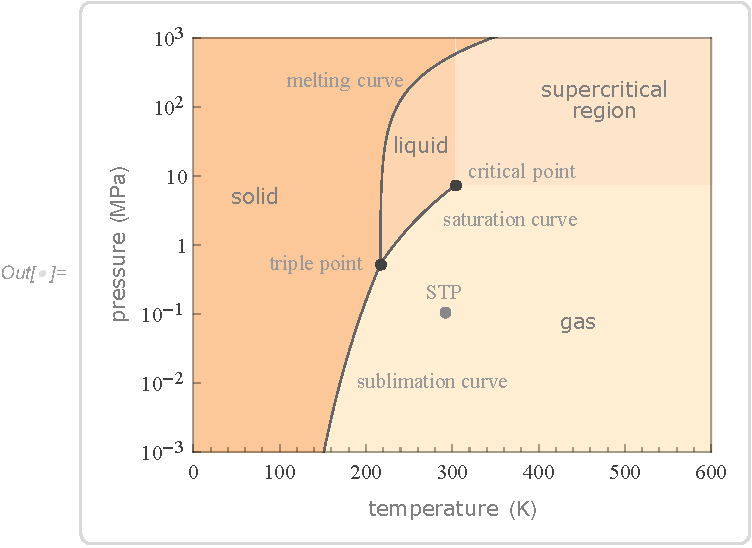
\includegraphics[width=\textwidth]{Figures/CO2PhaseDiagram}
\decoRule
\caption[The carbon dioxide phase diagram]{The phase diagram of carbon dioxide}
\label{fig:co2phase}
\end{figure}

The critical pressure of carbon dioxide is 304.12 K (31.10 °C) , and the
critical pressure is 7.39 MPa (72.9 atm). This temperature and pressure are easy
to achieve in the laboratory with standard chromatographic instrumentation, or
in an industrial plant with standard process engineering technologies.

Carbon dioxide is gaseous at ambient conditions. This means that once it has
been used in it's role as extractant, and it is exposed to the atmosphere, it
will rapidly evaporate, without needing added heat, and leaving no residues.

Any pure compound will have a supercritical point. Compounds with
technologically feasible supercritical points and useful chemical properties
include ammonia, methanol, CFCs/Freon, hydrocarbons (propane, butane), water and
sulfur hexafluoride. All of these lack green attributes: hyrocarbons pollute,
the CFCs deplete ozone, sulfur hexafluoride is a potent greenhouse gas, and
methanol and water are liquid at ambient conditions.

For these reasons the term supercritical fluid extraction is practically
synonymous with extraction using high-pressure carbon dioxide.

It is also possible to use supercritical fluids as reactants. This topic
falls outside the scope of this discussion.
 
\subsubsection{Modifiers}

\label{sec:modifiers}

The carbon dioxide molecule has zero dipole moment and the bulk fluid a low
dielectric constant, so supercritical carbon dioxide is expected to be
a non-polar solvent. (Although in practice the solvent behaviour is more
complex, partly explained by the high quadrupole moment of the carbon dioxide
molecule \autocite{Raveendran2005}.)

While the solvating power of a supercritical fluid is certainly `tuneable' by
adjusting its pressure and/or temperature, the range in solubility might be
quite limited in practice. Just as with other solvents, it is possible to add a
co-solvent or \keyword{modifier} to the supercritical carbon dioxide. This makes
it possible to increase the solubility of polar compounds in the supercritical
fluid. Methanol, ethanol, formic acid, and water are examples of suitable green
modifiers for carbon dioxide \autocite{Herrero2010}.

When modifiers are used the carbon-dioxide, modifier and solute forms a system
with four degrees of freedom (modifier percentage, solute concentration,
pressure, and temperature), which can become difficult to model. While this is a
challenge for process engineers who need to design efficient industrial systems,
analytical chemists can afford to be pragmatic and use heuristics to find
suitable conditions \autocite{Wells2003}.

\subsubsection{Practical extractions}

Figure \ref{fig:sfediagram} shows a schematic diagram of a system set up for
supercritical fluid extractions.

\begin{figure}
\centering
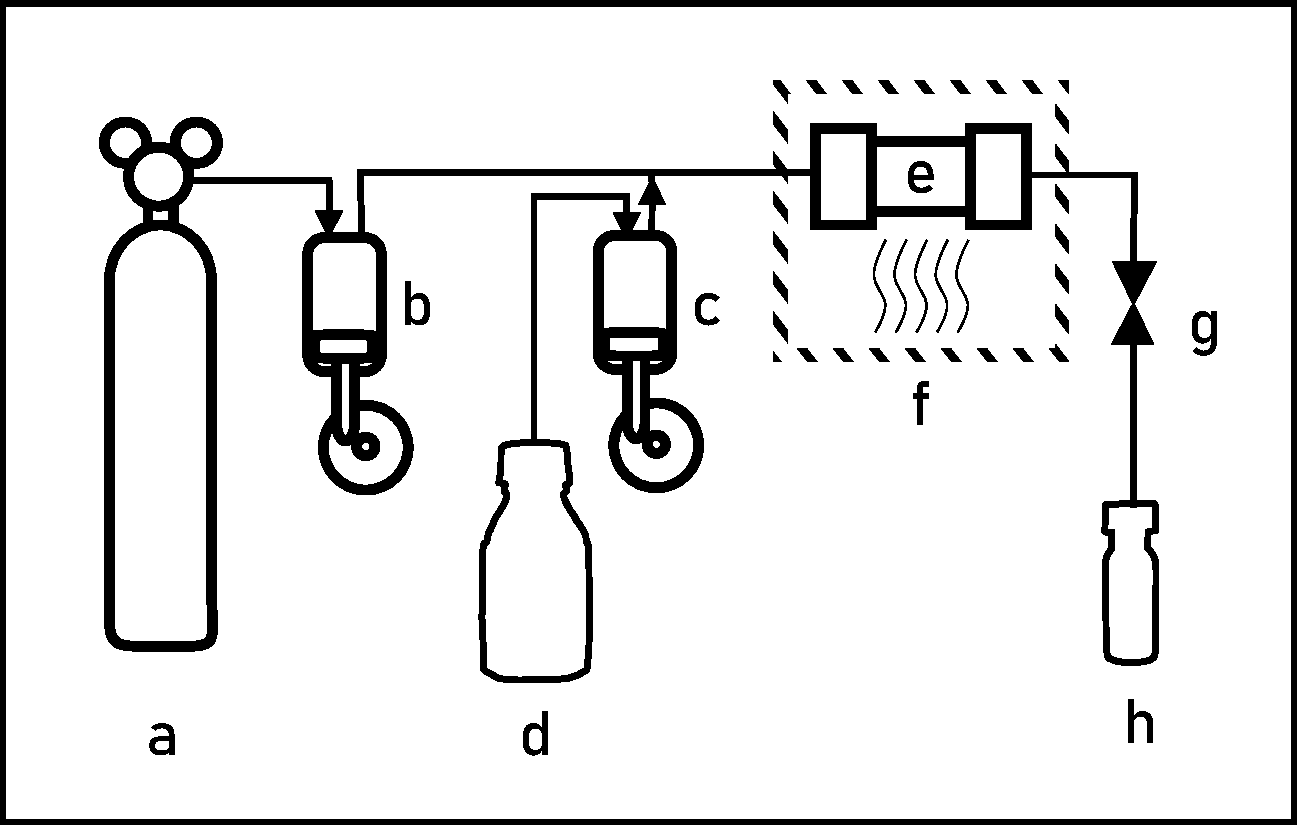
\includegraphics[width=\textwidth]{Figures/SFE_System}
\decoRule

\caption[SFE system diagram]{A diagram of an SFE system. (a) CO\textsubscript{2} supply (b)
High-pressure SF pump (c) High-pressure modifier pump (d) Modifier reservoir (e)
Extraction cell (f) Pressure control (g) Collection vessel}

\label{fig:sfediagram}
\end{figure}

Carbon dioxide (a) is readily available from suppliers of industrial gases, and
high-purity grades are available. Chromatography-grade solvents are usually used
as modifiers (d). High-pressure pumps (HPLC type) are used to compress the
carbon dioxide (b) and the modifier (c), which are mixed together at the
appropriate ratio. The mixture gets pumped into the (optionally heated (f))
extraction cell (e), which contains the material that needs to be extracted.
Having extracted the extract from the material, the supercritical fluid passes
through a pressure-control mechanism (g). This allows the pressure of the
supercritical fluid to drop to ambient, turning it into a low-density
non-solvating gas. The extract becomes desolvated, and precipitates in the
collection vessel (h). The operation of the system might be either static or
dynamic: in static operation the supercritical fluid is pumped into the system,
the flow is stopped, and the matrix/fluid mixture is given time to approach
equilibrium. Then the fluid is expelled and the extract collected.
In dynamic operation the supercritical fluid is pumped through the extraction
cell and the extract collected continuously. 


\section{Supercritical Fluid Chromatography}

An analyte will extract out of a matrix into a given solvent with a certain
efficiency and at a certain rate. While this is important while finding an
optimum extraction method, otherwise its relevance is limited.

However, \textit{different} analytes will extract out of a matrix with
\textit{different} efficiencies and at \textit{different} rates. In a 1906 paper
the Russian botanist Tsvet applied this observation to the dynamic extraction of
a bed of calcium carbonate that had mixture of plant pigments applied at the
inlet end, using petrochemical solvents. The different extraction efficiencies
and rates of adsorption and desorption on the calcium carbonate surface lead to
the \keyword{separation} of the compounds in the mixture. Tsvet called this
method of separation \keyword{chromatography} \autocite{Ettre1993,Ettre1993a}.
With time this method became generalized, and today chromatography is a major,
established scientific field with many ramifications and a myriad of
applications.

Because of the different technologies used in its applications, chromatography
is conventionally classed by the state of it's mobile phase as either
\keyword{gas chromatography} (GC) or \keyword{liquid chromatography} (LC).
However, as we have seen, solvating gases can also extract analytes from solid
stationary phases, and hence the term \keyword{supercritical fluid
chromatography} (SFC) was created for these kinds of separations.

\begin{figure}
\centering
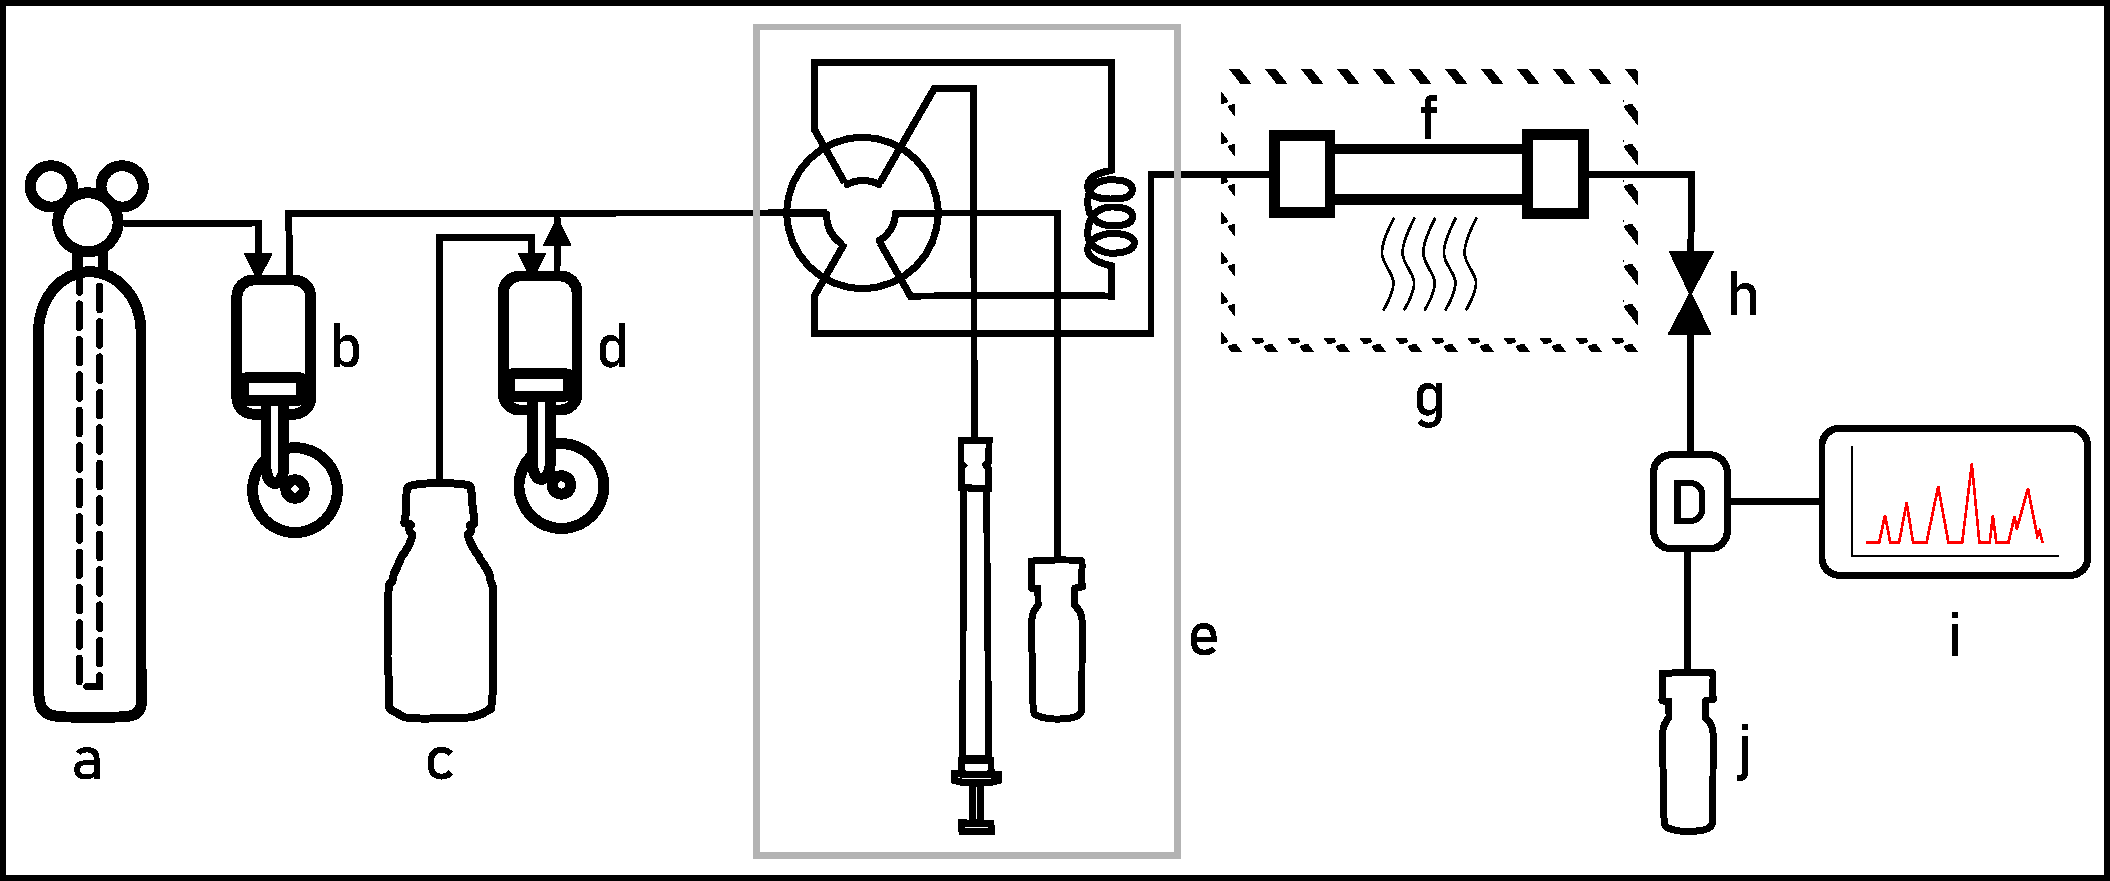
\includegraphics[width=\textwidth]{Figures/SFC_System}
\decoRule
\caption[SFC system diagram]{A diagram of an SFC system. (a) CO\textsubscript{2}
supply (b) High-pressure SF pump (c) Modifier reservoir (d) High-pressure
modifier pump (e) Injection system (f) Column (g) Optional heating (h)
Back-pressure control (D) Detector (i) Data system (j) Optional fraction
collection.}
\label{fig:sfcdiagram}

\end{figure}

Supercritical fluid chromatography as practised today bears a great resemblance
to \keyword{high performance liquid chromatography} (HPLC). The main reason for
this is that there is a large overlap between the technology used for HPLC and
the technology needed for SFC. In particular, both use high-pressure pumps and
columns packed with particles of very small diameter, and use optical
detectors. The same instrument manufacturers who supply HPLC instrumentation
also supply SFC instrumentation.

\subsection{SFC and FID}

But SFC was not always a technique based on HPLC technology. In the 1980s SFC
was practised using open tubular columns and flame detectors, so the instrument
designs looked more like GC instruments than HPLC instruments, and SFC was sold
as a replacement for GC \autocite{Poole2003}.

During this era the detectors used for SFC was the flame-based detectors used
for CG, in particular the flame ionization detector (FID).

The \keyword{flame ionization detector} was invented near-simultaneously in South
Africa and New Zealand \autocite{Ettre2008}. The core of the system is a
flame of hydrogen gas burning in pure air. The measured signal is the conductivity of
the flame plasma, which is measured by applying a {-100} V potential difference
between electrodes at the tip and the base of the flame. There are very few free
ions in the hydrogen flame, so the conductivity is normally low. But organic
compounds introduced into the flame creates a number of free ions, which
increases the conductivity of the flame gases. The change in conductivity is
measured by measuring the current between the two electrodes, using an electrometer. 

As a first approximation the signal produced by the FID is proportional to the
number of carbon atoms in the analyte. This is rather surprising, until the
mechanism of its working is elucidated. At high temperature in the hydrogen-rich
core of the flame, all hydrocarbon atoms are reduced to methane
\autocite{Holm1996}. Once it gets into contact with the hot oxygen in the outer
layers of the flame there is a chemi-ionization reaction. The electric field
acting on the ions creates a flow of ions, which can be measured as an electric
current.

\begin{figure}
\centering
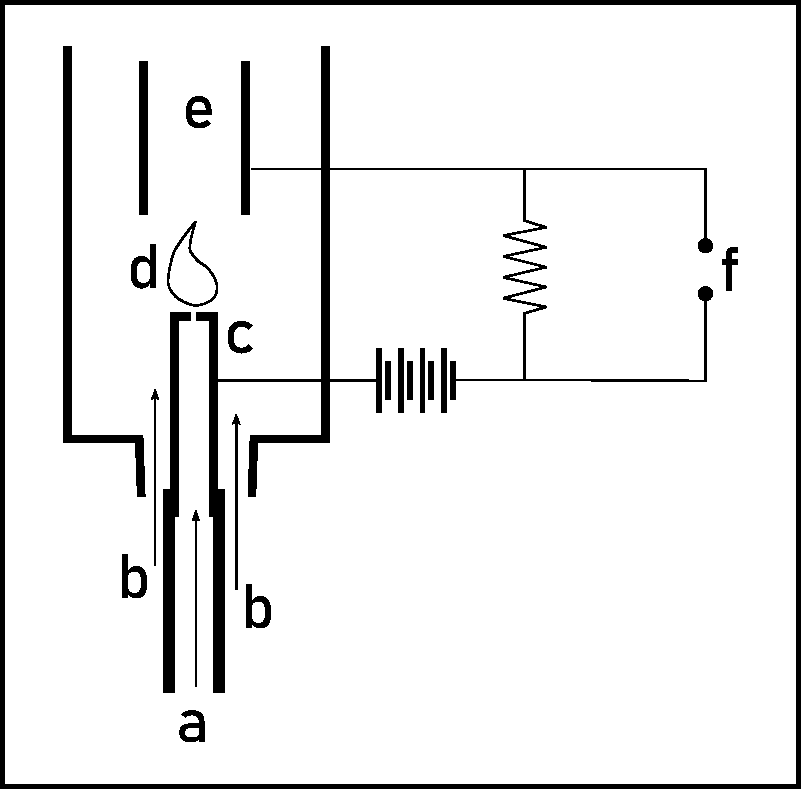
\includegraphics[width=\textwidth]{Figures/FIDSchematic.pdf}
\decoRule

\caption[FID diagram]{A schematic diagram of the flame ionization detector. (a)
Mixture of column eluate and hydrogen gas (b) Clean air (c) Metallic flame tip
electrode (d) Collector electrode (e) Conductivity signal}

\label{fig:fiddiagram}

\end{figure}

The FID's shining strength as a detector is its tremendous linear dynamic range
of 10\textsuperscript{7}. Combining the linear dynamic range with its carbon
sensitivity makes it an excellent detector for quantifying organic compounds.

During period of history that SFC was seen as a variant of GC, the FID was the
detector of choice. But when SFC started looking like HPLC, and the selectivity
of the chromatography started being manipulated by adding modifiers (see Section
\ref{sec:modifiers}), the FID lost its utility. The quantity of modifier added
to the carbon dioxide mobile phase swamps the FID detector, making it useless as
a detector. In contrast, if the chosen modifiers are transparent at the relevant
wavelengths, optical detectors are more useful in SFC using modified carbon
dioxide as a mobile phase.

\subsection{SFC×GC}
\label{sec:SFCxGC}
In chromatography, the analyte in the eluate can be detected to yield
information about the sample, or fractions of eluate can be collected for
further purification or characterization, or both. If fractions are collected,
there is nothing that prevents the chromatographer from subjecting a collected
fraction to another chromatographic separation.

For example, a synthetic chemist might use column chromatography to separate
their target compound from side-reaction compounds, collecting fractions of the
eluant. If the compounds are colourless, the chemist might use
\keyword{thin-layer chromatography} (TLC) to examine the fractions for presence
and purity of the relevant compounds.

If the product and the side-product were co-eluting it would not help to use the
same chromatographic system (\textit{i.e.} combination of stationary phase and
mobile phase) for the TLC examination, because the co-elution would not become
apparent. If, however, the chemist changed the mobile phase, or switched to a
different stationary phase for the TLC examination, then it is quite likely that
the two compounds would be separated. 

For example, if a synthesis involving sugars were being attempted, two sugar
enantiomers would likely co-elute on a silica clean-up column. Investigating the
sugar fraction using a TLC plate with a chiral stationary phase
would reveal the presence of stereoisomers.

The second, chiral separation (on TLC) is said to be \keyword{orthogonal} to the
first (packed column) separation.

Such a separation is an example of a two-dimensional (2D) separation. In
analytical chromatography, 2D separations are powerful tools.

The simplest 2D chromatography is called \keyword{heart-cutting}. In such a case
a fraction of interest is collected from the first dimension
(\textsuperscript{1}D) separation, and subjected to a second dimension
(\textsuperscript{2}D) separation. For example, a fraction collected from an
HPLC separation could be injected into a gas chromatograph. The separation on
the GC dimension would obviously be very different from the separation on the
HPLC dimension, and therefore we can say that the orthogonality is high.

Heart-cutting is a useful way to get detailed information from a sample, but it
is technically demanding and labour-intensive. It is usually employed for
challenging separations in well-understood samples, because peaks of interest
in the first dimension must be captured for injection on the second dimension.

If, however, one collects the eluate in equal fractions and do identical
separations on each of the fractions, then one enters the domain of
\keyword{comprehensively coupled chromatography}. The comprehensive coupling of
orthogonal chromatographies does not demand a previous understanding of the
sample, and doing exactly the same separation for each fraction allows the
process to be automated.

A 2D separation can be called comprehensive if the following three criteria are
met \autocite{Giddings1987}:

\begin{enumerate}
  \item Every part of the sample is separated by two distinct chromatographic processes.
  \item Equal percentages of all sample fractions are separated by the second process.	 
  \item Compounds resolved by the first dimension separation remains resolved.  
\end{enumerate} 

To effectively distinguish between heart-cut and comprehensive 2D couplings, a
terse nomenclature was developed. Simple coupling between systems is
designated by a hyphen (``-''), for example HPLC-GC. This corresponds to the
usual notation of a coupled detector coupled to a chromatograph, for example
GC-FID or GC-MS. Comprehensive coupling is denoted by a multiplex sign
(``$\times$''), for example GC$\times$GC. If it is not clear from the context,
the detector can be specified using a hyphen, as in GC$\times$GC-MS.

Of the comprehensive coupled chromatography techniques, GC$\times$GC is the most
mature, with a selection of powerful instruments on the market.

This thesis further explores the implementation of SFC$\times$GC, as first
developed by Venter and Rohwer \autocite{Venter2004, Venter2006}.

In this implementation of SFC$\times$GC, fractions of the eluate of the SFC is
transferred to the GC. The mobile phase is changed from carbon dioxide to
hydrogen in the modulating interface, and the GC dimension is a conventional open-tubular
capillary separation with FID detection.

Any volatile modifiers or additives added to the SFC mobile phase will be separated from
the analytes by the GC dimension. This makes in possible to use the FID as a detector
in an SFC$\times$GC chromatograph where the SFC is based on HPCL technology.

The \textsuperscript{2}D separations are \keyword{fast} chromatographic
separations, \textit{i.e.} separations optimized for speed, sacrificing
resolution. This is achieved using fast temperature programming of the GC
separation.

The high orhtogonality of the SFC and the GC separations enables novel comprehensive 2D
chromatography, which we applied to the chemical analysis of biodiesel.
 
% Chapter 3

\begin{savequote}[\quotewidth]
The nice thing about standards is that you have so many to choose from.
\qauthor{Andrew S. Tanenbaum}
\end{savequote}


\chapter[Biodiesel standards]{Biodiesel, technical standards and chemical analysis} % Main chapter title

\label{Chapter3} % For referencing this chapter elsewhere, use \ref{Chapter3}

\section{Introduction to standards}
\label{Sec:Intro}

The fact that vegetable oil can be used to fuel Diesel engines has been known
since the earliest days. Rudolf Diesel himself had exhibited an engine at the
Paris Exhibition in 1998 \autocite{Knothe2010} that ran on peanut oil. But the
development of the petroleum industry late in the 19th century ensured an ample
supply of fossil fuel for these engines.

The development of the diesel engine happened in parallel with its fuel, for, as
Cummins said ``\ldots we must never forget that \textit{an engine and the fuel
it consumes are inseparable partners}; the one cannot progress without the full
cooperation of the other'' \autocite{Cummins1989}. The first invention of an
engine presupposes a supply of fuel, but the variation-selection process that
searches for lower costs and higher efficiency then opens up the quest for more
fuels. If a possible fuel is found, meticulous engine builders would then have
to test each new fuel in their engines and approve of it. But fuel suppliers
would like to see their fuels used in as many engines as possible. This
convergence of interests gives rise to the establishment of \textit{technical
standards}. Technical standards allow engine builders to develop engines that
will run on any fuel with certain agreed-upon standard qualities, and fuel
producers can produce fuels knowing that they will work on any engine designed
for that fuel.

A technical standard or just \textit{standard} is a ``document, established by
consensus and approved by a recognized body, that provides, for common and
repeated use, rules, guidelines or characteristics for activities or their
results, aimed at the achievement of the optimum degree of order in a given
context'' \autocite{Hatto2010}. Standards are used in many aspects of
industrialized societies, from implantable medical devices \autocite{ISO2019} to
coffins and caskets \autocite{SABS1993}. Standards are often associated with
products, but also apply to procedures \autocite{ISO2015} and systems
\autocite{ISO2017}.

Standards are not mandatory, nor do they provide the `best' way of doing
something. The great strength of standards is their reliability.
``Standards exist principally to provide a reliable basis on which common
expectations can be shared regarding specific characteristics of a product,
service or process'' \autocite{BSI2016}.

Standards are published by \textit{standards organizations}, which might
be national or international in character, or might be established to serve a
certain industry. Standards organizations are often known by their
abbreviations, and a few of them are listed in Table
\ref{tab:StandardsOrganizations}. The authors of these standards documents are
usually \keyword{technical committees}, comprised of individuals from a wide
variety of stakeholder organizations, who work towards consensus.

\begin{table}
	\caption{A few well-known standards organizations}
	\label{tab:StandardsOrganizations}
	\centering
	\begin{tabulary}{\textwidth}{LLL}
	\toprule
	\tabhead{Abbreviation} & \tabhead{Name} & \tabhead{Country of origin} 		\\
	\midrule
	SABS 	& South African Bureau of Standards 		& South Africa	\\
	ISO		& International Organization for Standardization & International \\
	CEN 	& European Committee for Standardization 	& Europe		\\
	ASTM 	& ASTM International 						& USA			\\
	BSI	 	& British Standards Institution 			& UK			\\
	IEC 	& International Electrotechnical Commission & International \\
	DIN 	& German Institute for Standardization 		& Germany 		\\
	ANSI 	& American National Standards Institute 	& USA 			\\
	UL 		& Underwriter's Laboratory 					& USA 			\\
	ITU 	&International Telecommunication Union		& International \\
	\bottomrule\\
	\end{tabulary}
\end{table}

Standards have a unique publication system. They are not published by publishing
houses, but by the standards organizations themselves, who sell the documents
directly to end users. Each standard is usually also better known by its number
than by its title. For example, if I were to mention the document entitled
``Quality management systems — Requirements'' few people would know that I'm
talking about the well-known quality system standard usually known as ISO 9001.

The South African national standards body is the South African Bureau of
Standards (SABS), which was established by an act of parliament,
 Standards Act, 1945 (Act No. 24 of 1945)), as amended by the Standards Act, Act
 No. 8 of 2008 \autocite{Act8-2008}. The SABS issues South African National
 Standards.

Standards organizations not only write standards, they might also
\keyword{adopt} them. Adoption happens when a suitable standard has already been
issued by another standards organization. Standards very often refer to other
standards, and standards are often based on published research. While standards
are not mandatory, some legislation might refer to standards. 

The desire for engine designers for access to a reliable fuel and for fuel
suppliers to have the largest possible market lead them to cooperate in the
development of standards for fuels. In South Africa the relevant standard for
petroleum-based diesel fuel is SANS 342, and in the USA the equivalent is ASTM
D975. According to the Petroleum Products Act of 1977, as amended, diesel fuel
sold to an end-consumer must conform to SANS 342

Biodiesel is chemically very different from \keyword{petrodiesel} (diesel
derived from fossil sources), and therefore the technical standards of biodiesel
need to be different from the standards for petrodiesel.

\section{SANS 1935: An overview}

The current South African standard applicable to biodiesel is ``South African
National Standard 1935 Automotive biodiesel — Fatty Acid Methyl Esters (FAME)
for diesel engines — Requirements and test methods'' \autocite{SANS1935}. This
is an adoption of the European Committee for Standardization's (CEN) standard EN
14214 \autocite{EN14214}. In the USA is the equivalent standard is ASTM D 7651,
which is largely similar but of different heritage.

SANS 1935 consists of 18 pages. The first two pages are unnumbered: for the
purposes of this discussion they will be numbered in small Roman numerals.

\begin{description}


\item[p(i)]{The first page is a title page, following the usual format for SABS
standards. The top line of the page contains the ISBN (978-0-626-26349-2), and
in large type the standard number (SANS 1935:2011). Then follows in capital
letters ``South African National Standards'', and below that the title
``Automotive biodiesel --- Fatty Acid Methyl Esters (FAME) for diesel engines
--- Requirements and test methods''. At the bottom edge of the page we find the
SABS logo and some contact information.}

\item[p(ii)]{The second page is an informational page. It starts with a table of
changes, which was still empty at the time of writing. Then follows a foreword,
in which the technical committee who approved the standard is acknowledged
(National Committee SABS SC 1018A). It also gives the date of publication
(December 2011) and states that it supersedes SANS 1935:2004. Then there is a
very significant line, which states that the standard is referenced in the
Petroleum Products Act \autocite{Act120-1997}. }
	
\item[p1]{Contains the Table of Contents} 

\item[p2]{Is left blank}

\item[p3]{Paragraph 1: This paragraph describes the scope of the standard, which
is that it applies to biodiesel as an automotive fuel.} 

\item[p3]{Paragraph 2:
This paragraph lists all the normative standards required to comply with SANS
1935. Thirty-five standards are listed.}

\item[p4]{Continues the list of normative references}

\item[p5]{Paragraph 3: This paragraph contains a list of definitions. The most
important one is this: ``biodiesel [is a] fuel comprised of methyl esters of
long chain fatty acids derived from vegetable oils.'' This is a very specific
description of biodiesel. It excludes animal fats as a source of fatty acids,
and it excludes \em{ethyl} esters. But a note reads ``Consideration for the
inclusion of ethyl esters, animal fats and C8 – C12 carbon chains should be
taken later.'' The significance of ethyl esters is that methyl esters are not
usually ``carbon neutral'', that is, he methanol used in the transesterification
reaction is usually obtained from the petrochemical industry, whereas ethanol
from fermentation (See Section \ref{sec:BioEthanol}) could be carbon neutral.
The definition also rules out hydrotreated vegetable oil (see Section
\ref{sec:GreenDiesel}) or biomass-derived Fischer-Tropsch diesel (see Section
\ref{sec:FT}.}

\item[p5]{Paragraph 4: This paragraph lists requirements} 

\item[p5]{Paragraph 4.1 discusses general requirements. According to these
requirements biodiesel is a homogeneous liquid, free of adulterants or
contaminants, to which additives might be added. It provides details regarding
testing for oxidative stability and cold-flow properties}

\item[p6]{Paragraph 4.2: This paragraph is about physical and chemical
properties and states that biodiesel shall comply to the requirements of Table
1}

\item[p7]{Paragraph 4.3: This paragraph concerns methods of test. It states that
test methods shall be  one of the test methods listed in Table 1.}

\item[p7]{Paragraph 4.4 concerns disputes. It comes into effect when there is a
dispute about product quality between, say, a biodiesel manufacturer and a
biodiesel distributor. The contents of this paragraph prescribes which reference
method shall be used.}

\item[p7-p8]{These pages contain Table 1.}

\item[p9]{Paragraph 5 describes a few simple rules for packing and marking biodiesel.}

\item[p10-p11]{Annex A describes a method for the calculation of iodine value
from chromatographic data. This calculation might be used instead of a direct
measurement of the iodine value.}

\item[p12]{Annex B prescribes how samples for testing must be taken.}

\item[p13]{Annex C gives a list of values for calculating precision.}

\item[p14]{Annex D provides an approved method for correcting density
measurements. The prescribed tests requires density to be measured at
\SI{15}{\celsius}, which might be inconvenient. Instead, a different test may be
made at a more convenient temperature, and a correction applied. }

\item[p15]{Annex E is informative and recommends the implementation of quality
management systems. It is followed by a bibliography.}

\item[p16]{The final page contains information about the SABS and its services.}

\end{description} 

\section{SANS 1935: Properties, requirements and methods.}

On studying SANS 1935, it quickly becomes clear that the core of the document
is Table 1. This table has three columns. The first column lists a
\keyword{property}, the second column specifies a numerical value the property
has to conform to, the \keyword{requirement}, and the third column prescribes
the \keyword{test method} that must be used to obtain the value.

In the following discussion each of the requirements will be discussed, in order
of increasing relevance to this thesis, grouped by method of determination (See
Figure \ref{fig:MindMap}).


\begin{figure}
\centering
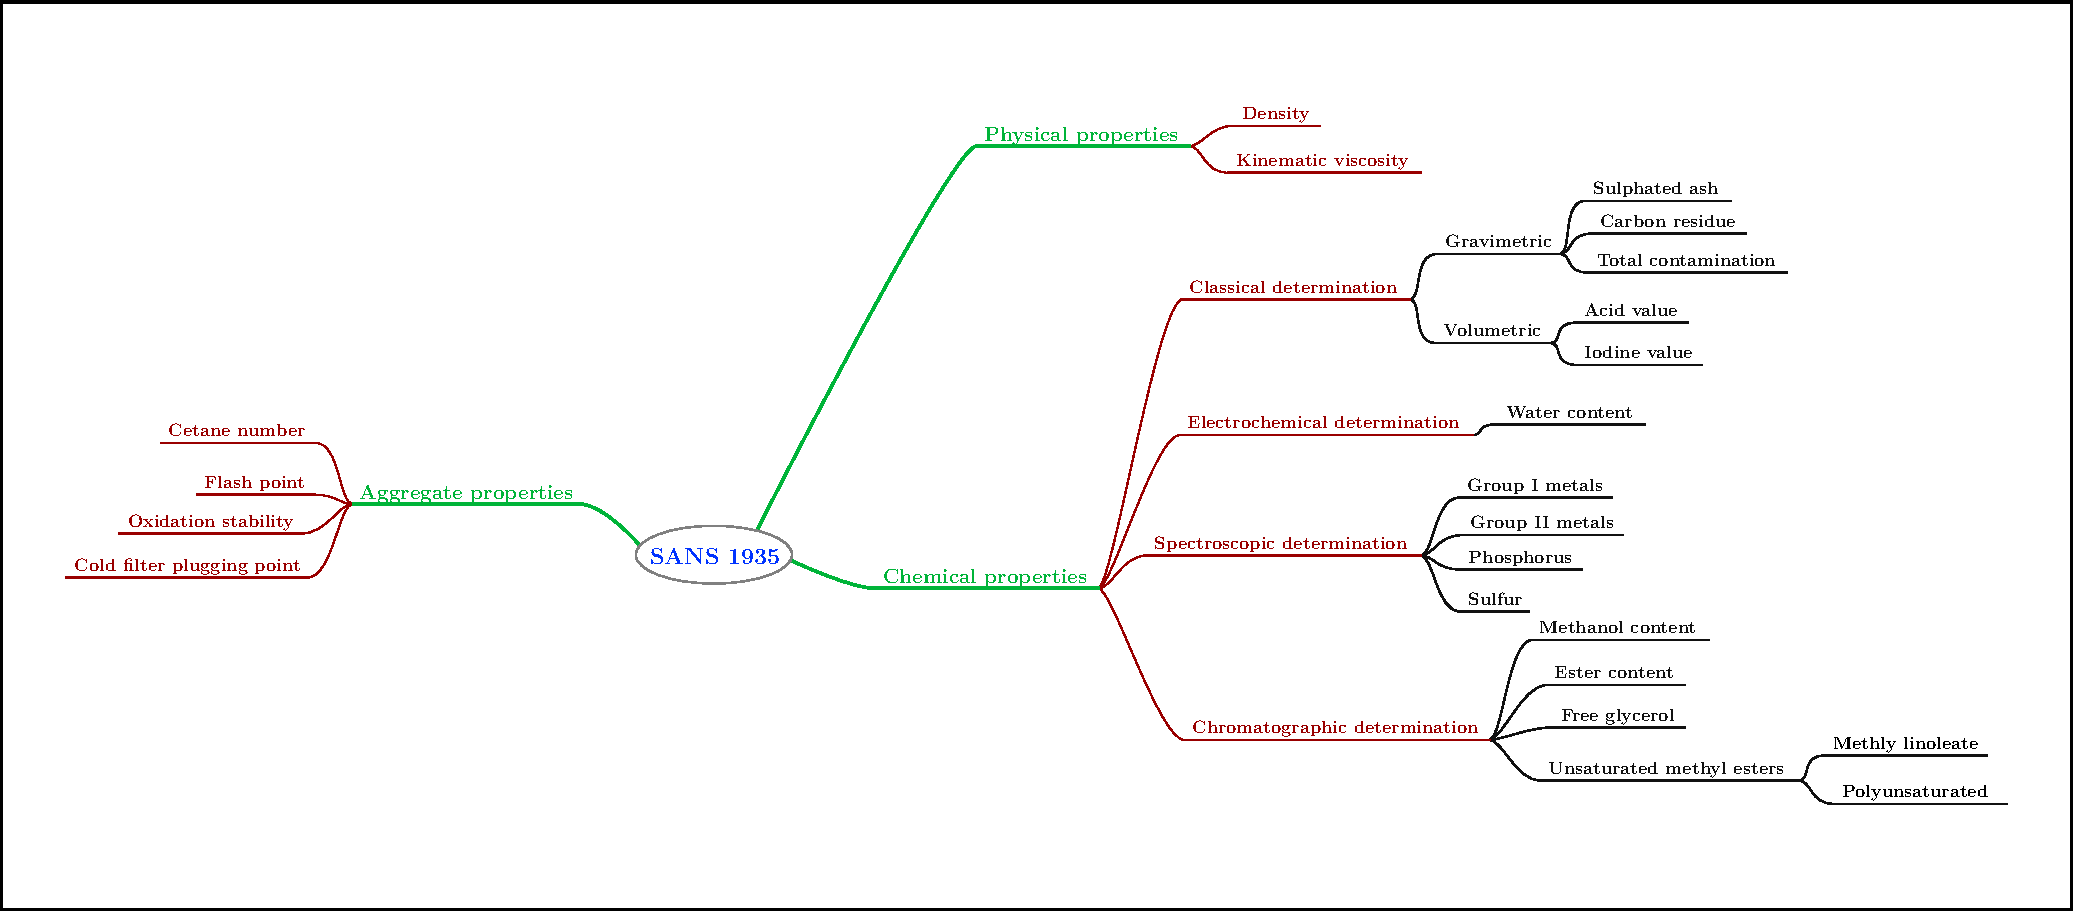
\includegraphics[width=\textwidth]{Figures/SANS1935.pdf}
\decoRule

\caption[Discussion of SANS 1935.]{A mind map showing how the properties of
biodiesel assessed by SANS 1935 is grouped for the purpose of discussion in this
chapter.}

\label{fig:MindMap}
\end{figure}

\section{SANS 1935: Physical properties}

\subsection{Density}

A diesel engine can only deliver work proportional to the heat of combustion of
the fuel, and for a given chemical composition the energy will be proportional
to the mass of the fuel. But diesel engines inject measured volumes of fuel, not
measured masses. (Fuel is also sold by volume, not mass.) Therefore, an engine
designer must specify the density of the fuel to specify the power output of the
engine.

According to SANS 1935 the density of biodiesel is required to be
\SIrange{860}{900}{\kilogram\per\cubic\metre} at a temperature of
\SI{15}{\celsius}. The testing methods that can be used are described in ISO
3675 and ISO 12185.

ISO 12185 prescribes the measurement of density by using an electronic
instrument known as the oscillating tube density meter. This measures the
density of a liquid by measuring the frequency of a freely-oscillating tube
filled with the liquid under test. The frequency depends on the mass of the
filled tube, and therefore on the density of the liquid.
These devices are easy to use and very accurate. The temperature of the liquid
is controlled electronically.

ISO 3675 prescribes the use of a hydrometer, which is an instrument that
measures density by measuring the buoyant force on a floating indicator.
According to the law of Archimedes, the buoyant force on a body immersed in a
liquid is equal to the weight of the displaced liquid. If the liquid is denser,
the force is greater. Therefore, in a denser liquid a floating indicator will
float with more of the indicator above the surface of the liquid. Hydrometer
technology is mature, and the devices are simple and robust.  If ISO 3675 is
used at a temperature other than the specified one, a temperature correction is
applied, as described in Annex D.

\subsection{Kinematic viscosity}

The viscosity of a fluid is a measure of its resistance to flow when a force is
applied to it. Kinematic viscosity is the resistance to flow of a liquid when
the force of gravity is applied to it. This flow of course depends on the
density of the liquid, so that kinematic viscosity is determined by measuring
the liquid's viscosity and dividing it by its density. It is important that a
diesel fuel have the right viscosity, because the fuel must be finely divided
for rapid combustion. The size of the droplets of fuel in the spray produced by
the engine's injectors is strongly influenced by the fuel's viscosity.

SANS 1935 requires that kinematic viscosity be
\SIrange{3.5}{5.0}{\milli\metre\squared\per\second}. The measurement method is
specified by ISO 3104, which uses a capillary viscometer: the time taken for a
fixed volume of liquid to flow through a capillary. This time is them multiplied
by an instrument-specific factor to yield the kinematic viscosity.

\section[SANS 1935: Aggregate properties: Specialized in\-stru\-mentation]{SANS
1935: Aggregate properties: \\ Specialized in\-stru\-mentation}

Some of the requirements specified in SANS 1935 are not values that have direct
correspondence to physical or chemical quantities usually used in science, but
are measures that have proved useful in engineering practice.

\subsection{Cetane number}

For a diesel engine to operate according to design the fuel must combust in a
reliable manner. The cetane number is a number that indicates the ease of
ignition of a fuel in a diesel engine. Cetane is a synonym for hexadecane, and
is a liquid compound that ignites easily when injected into a diesel engine at
high compression and temperature, without a spark. In contrast, its highly
branched isomer 2,2,4,4,6,8,8-heptamethylnonane (also called isocetane, see
Figure \ref{fig:Cetane}) ignites less easily. The intuitively-understood ``ease
of combustion" can be quantified as the \keyword{ignition delay}, the time
between the moment the fuel is injected in to the engine and the moment the
ignition starts. A mixture of the two compounds will have an ignition delay
somewhere between that of the two compounds. A higher number indicates easier
ignition.

\begin{figure}
\centering
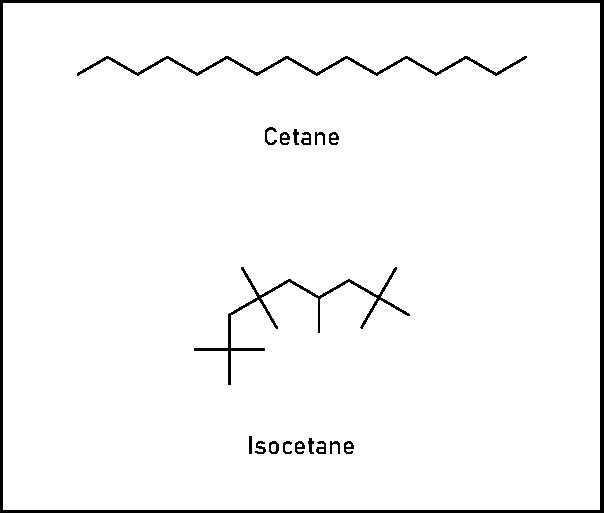
\includegraphics[width=0.8\textwidth]{Figures/cetane.pdf}
\decoRule

\caption[Cetane and isocetane]{The chemical structures of the C16 hydrocarbon
isomers cetane and isocetane.}
\label{fig:Cetane}
\end{figure}

SANS 1935 prescribes the test method of ISO 5165. The cetane number is obtained
by measuring the ignition delay in a highly specialized test engine. The engine
is equipped with the necessary instrumentation to measure ignition delay. It is
a single-piston, four-stroke engine that has a combustion chamber of variable
volume, which gives it a variable compression ratio. While running on the fuel
under test, the compression ratio is changed until a prescribed ignition delay
is achieved. Then the cetane/isocetane mixture that will give the same ignition
delay at that compression ratio is found. If pure cetane will give the
prescribed ignition delay, then the cetane number 100 is assigned. If pure
isocetane gives the prescribed ignition delay, then the cetane number 0 is
assigned. If it is found that a 50:50 cetane:isocetane mixture produces the
prescribed ignition delay, then the cetane number of 50 is assigned.

Cetane number gives limited insight into the chemical properties of the fuel, or
indeed, engine performance. But it is a trusted measure of the suitability of a
fuel for use in a diesel engine and is therefore included in the standard.
Biodiesel from common feedstocks usually easily meets the cetane specifications.

\subsection{Flash point}

Fuels are, naturally, flammable, and different fuels are flammable to different
degrees. A fuel's \keyword{flash point} can be used to quantify its degree of
flammability. The flash point is the temperature at which a fuel's vapour at
atmospheric pressure will ignite when it comes in contact with a flame.

The measurement of flash point is not primarily concerned with the performance
of the fuel inside the engine, but is important to know because it determines
how the fuel can be safely be handled during transport and storage
\autocite{WFCC2009}.

SANS 1935 specifies that either ISO 2719 (Procedure A) or ISO 3679 be used for
determining the flash point. It seems that this aspect of SANS 1935 is out of
date, because ISO 2719:2002 has been withdrawn and revised by ISO 2719:2016,
which adds a Procedure C, specifically for FAME. ISO 2719 specifies the use of a
Pensky-Martin closed-cup test, an automated device in which a temperature ramp
heats an enclosed amount of liquid, while an ignition source is periodically
introduced. The temperature at which the vapour ignites is the flash point. ISO
3679's test procedure works on a similar principle, but the device uses a
smaller volume of liquid, and the liquid and its vapour are considered to be in
thermal equilibrium.

\subsection{Oxidation stability}
\label{sec:Rancimat}

Fossil fuels for diesel engines are largely composed of alkanes, which are
chemically very inert. This means that they can be stored for long periods
without significant degradation. Biodiesel, in contrast, is by definition
\autocite[Paragraph 4.1.1]{SANS1935} mostly composed of fatty acids, which are
less inert than alkanes. This instability has been known since antiquity as
fatty food going \keyword{rancid}. In particular, double bonds in the fatty
acids are liable to reactions with atmospheric oxygen \autocite{Velasco2010}.
These are free radical reactions, illustrated in Figure \ref{fig:RancidRadical}.
The hydroperoxides that form are highly reactive and can react with other fuel
compounds to form polymers, soaps and acids.

\begin{figure}
\centering

\includegraphics[width=0.8\textwidth]{Figures/1281px-Lipid_peroxidation.png}
\decoRule

\caption[The peroxidation of lipids.]{The peroxidation of lipids. By Tim
Vickers, after \autocite{Young2001}. Public Domain,
\url{https://commons.wikimedia.org/w/index.php?curid=1728531}}

\label{fig:RancidRadical}
\end{figure}

The oxidative stability is measured by the Rancimat, an automated instrument. In
operation it bubbles a stream of hot air through a sample of biodiesel. This air
then passes through a conductivity measuring cell filled with deionized water.
The conductivity of the water increases when volatile acids dissolve in it. At
the beginning of the test period very few acids are swept into the water, so the
conductivity remains low. As the sample oxidizes and produces acids, the
conductivity of the water slowly increases. But the oxidation reaction is
\keyword{autocatalytic}, which means that the products of the oxidation reaction
accelerates the oxidation. The result of the autocatalysis is that there is a
sudden increase in conductivity on the conductivity curve. The time taken until
this point is reached is called the \keyword{induction period}.

SANS 1935 requires a minimum induction period of 6 minutes at
\SI{110}{\celsius}. Paragraph 4.1.2 permits the addition of antioxidants,
compounds that prevent oxidation.

\subsection{Cold filter plugging point}

The flow of a liquid depends on its temperature. Most obviously, its viscosity
depends on the temperature. But a liquid can freeze, which will also influence
its flow. The operating temperature of a diesel engine is so high that the
temperature of the fuel in the engine will be high enough to guarantee adequate
flow for injection, but the biodiesel needs to be pumped from the fuel tank,
through a fuel filter, to the engine. If crystals of fuel form at low
ambient temperatures, these crystals might plug the pores in the filter, which could
lead to fuel starvation in the engine. It is therefore important that the
biodiesel must be able to be pumped through the engine's fuel filter at all
expected temperatures.

For this purpose SANS 1935 specifies a \keyword{cold filter plugging point},
measured according to SANS 50116. It is the lowest temperature at which a given
volume of biodiesel still passes through a standardized filtration device in a
specified time when cooled under certain conditions. 

\subsection{Copper strip corrosion}

Many fuel storage  and transfer systems parts and engines parts are made of
metals, and under adverse conditions those parts are susceptible to corrosion.
Corrosion accelerates in chemical environments that include, \textit{inter
alia}, acids, water and oxygen, but corrosion is a complex process, so it is
very difficult to predict which combination of factors will result in
unacceptable corrosion.

SANS 1935 prescribes ISO 2160 as the test for corrosiveness. In this test a
strip of pure copper metal is polished and then immersed in a sample of the
biodiesel at \SI{50}{\celsius} for \SI{3}{\hour}. The degree of corrosion is
judged by visually comparing it to a standard card and then assigning it to a
corrosion class.

\section{SANS 1935: Chemical properties: Classical determination}

\subsection{Sulfated ash}

Ash is the solids remaining after the complete combustion of a fuel. This is
measure of the solids that will remain after use. Ash might originate from
suspended solids, soluble metallic soaps, and residual catalyst that form
refractory oxides during combustion. In addition to wear and deposits in the
fuel system associated with ash, it also impairs modern diesel particulate
filters.

SANS 1935 specifies ISO 3987 for the determination of sulfated ash. For the
determination of ash it would not be practical to actually combust the sample
and weigh the residue, because the ash might be carried away, either as volatile
species or as a finely divided aerosol. Therefore the sample is oxidized using
sulphuric acid, and then heated to drive off the sulphuric acid. What remains is
metal oxides, which can be weighed.

\subsection{Carbon residue}

When a mixture of organic compounds is heated under conditions of low oxygen, it
can form coke. Coke is a material that is practically pure carbon. Pure, solid
carbon will combust, but the reaction is kinetically limited, so it will only
combust slowly under conditions of high temperature and a large excess of
oxygen. If a fuel tends to form coke inside an engine, it can cause problems in
operation. Vegetable oil as diesel fuel, for example, tend to form coke on the
injectors \autocite{vanderWalt1982}. This coking can cause problems with injection,
which would affect engine performance. Carbon residue is not a scientific
measure: from long experience it has been found to correlate with coking
tendencies of oils in the petroleum industry, and so found its way into the
biodiesel standard.

The test method prescribed for testing for carbon residue is ISO 10370. This
involves heating a sample of biodiesel to high temperature in a crucible in air,
using standardized apparatus. Most of the sample burns off, leaving a residue.
The mass of the residue is determined and reported.

\subsection{Total contamination}

Ideally, biodiesel should be a homogeneous liquid. Some undissolved material can
be tolerated, but too much can plug filters. The amount of undissolved solids is
termed \keyword{total contamination}

The test of total contamination specified by SANS 1935 is contained in SANS
52662, which is synonymous with EN 12662. In this test total contamination is
determined by obtaining the mass of material retained on a glass-fibre filter
after passage of the biodiesel sample.

\subsection{Acid value}

The end products of oxidative degradation of biodiesel include free organic acids, so the
acidity of biodiesel is a good indicator of its quality. Measuring the acidity
gives an indication of how much the biodiesel has already oxidized, whereas the
oxidation stability (measured by Rancimat, see Section\ref{sec:Rancimat})
indicates how well the biodiesel will withstand oxidation on storage.

SANS 1935 specifies the test described in SANS 54104, which is equivalent to EN
14104. This test is a titration with alcoholic KOH of a sample of biodiesel
dissolved in a mixture of solvents. A glass pH electrode connected to an
electronic pH meter is used to follow the titration.

\subsection{Iodine value}

As discussed above (see Section \ref{sec:Rancimat}) the oxidation of biodiesel
is a major quality concern. The tendency of biodiesel to oxidize correlates with
the number of double bonds in the fatty acids, or their \keyword{degree of
unsaturation}.

% t AOCS method Cd 1d-92 using cyclohexane-acetic acid (also used by the
% European standard EN 14111) as solvent system are based on the Wijs solution.

The degree of unsaturation of oils and fats have long been measured by the
\keyword{iodine value}, dating from 1884 \autocite{Knothe2007}. Halogens will
rapidly add to double bonds, so that when a mixture of fatty acids is treated
with a known excess of iodating reagent, the remaining iodine can be titrated to
determine the amount of iodine absorbed by the fatty acids. The iodine value is
the mass of iodine absorbed by 100 mass units of fat or oil.

The relevance of including iodine value in biodiesel standards has been
questioned \autocite{Knothe2002}, because all the information regarding
unsaturation of the fatty acids in biodiesel is contained in chromatographic
data which need to be obtained in other requirements. SANS 1935 seems to
acknowledge this, because Annex A allows that the iodine value can be calculated
from chromatographic results (see Section \ref{sec:ChromDetUnsat}).

Because determining iodine value is a mature technology and therefore relatively
simple, it is tempting to think of it as a test that might be useful to small
biodiesel producers. Unfortunately the iodine value is determined by the
feedstock, so that for a feedstock from a certain vegetable oil crop there is
unlikely to be any significant variation in iodine value, no matter the
production process. Iodine value might be useful as a simple indicator of
feedstock quality when the biodiesel is produced from waste vegetable oil, which
might contain a variety of oils from different origins.

The prescribed method for the requirement is SANS 54111 (or, equivalently, EN
14111). In this method a known excess of Wijs's reagent (iodine chloride in
acetic acid) is added to a weighed sample. The reaction mixture is then treated
with potassium iodide, which converts the excess ICl to I\textsubscript{2},
which is then titrated with potassium thiosulfate. The titration is followed
potentiometrically and the equivalence point determined from the titration
curve.

\section{SANS 1935: Chemical properties: Electrochemical determination}

\subsection{Water content.}

The compounds that comprise biodiesel are much more polar than those of
petro\-diesel. Therefore, much more water can dissolve in biodiesel than can
dissolve in petrodiesel. This water has several deleterious effects on the
quality of biodiesel. It encourages the growth of micro-organisms, allows
hydrolysis, and accelerates corrosion.

The level of water specified in the requirements of SANS 1935 is lower than the
solubility of water, and therefore refers to dissolved water. Free, visible
water is excluded by paragraph 4.1.4.

The method specified by SANS 1935 for the determination of water in biodiesel is
ISO 12937. This standard prescribes the well-known Karl Fischer titration used
for the determination of water in solvents. This is a \keyword{coulometric}
titration, which means that electricity is used as titrant. The titration curve
is a plot of oxidation potential of a platinum electrode against the amount of
charge (current integrated over time). 



\section{SANS 1935: Chemical properties: Spectroscopic determination}

\subsection{Group I metals}

The most common catalysts in biodiesel production are sodium or potassium
hydroxides (NaOH and KOH) or alkoxides (CH\textsubscript{3}ONa and
CH\textsubscript{3}OK). These catalysts are polar and will dissolve in the
glycerol byproduct of biodiesel production. But some may remain in the biodiesel
itself, and needs to be removed. This cleanup can be done by washing with water,
adsorbent columns, or selective membranes \autocite{Atadashi2011}.

SANS 54108 is the method specified for the determination of sodium, and SANS
54109 the method specified for potassium. Both are flame atomic absorption
spectroscopy methods: a sample of the biodiesel is aspirated into a gas flame,
where the sodium and potassium are atomized. The atoms will absorb light at
certain wavelengths, and measuring the amount of light absorbed will give a
measure of the amount. Alternatively, EN 14538 may be used to determine sodium
and potassium simultaneously with calcium and magnesium (see Section
\ref{sec:GroupIIMetals}).

\subsection{Group II metals}
\label{sec:GroupIIMetals}

Fatty acids neutralized by alkali and alkaline earth metal hydroxides form
\keyword{soaps}. If these metals are present in the feedstock, as catalyst, or
in washing water they can form soaps with the fatty acids in the biodiesel.
These soaps can form deposits in engines that can affect operation. For
example, deposits of calcium soaps have been reported to cause injectors to
stick \autocite{Pischinger2000}.

SANS 1935 prescribes EN 14538 as the method for determining Group II metals.
This is an optical emission spectroscopy method: a sample of the biodiesel is
diluted in kerosene, and injected into a inductively coupled argon plasma. The
emission intensities at certain wavelengths are compared to the emission
intensities of solvents containing known concentrations of the metals.

\subsection{Phosphorus}

Phosphorus expected in biodiesel should not affect a diesel engine's
performance, but it can have a detrimental effect on the exhaust treatment
system by forming ash that can clog filters and reactive species that can reduce
catalyst effectiveness. Trace levels of phosphorus will be expected in
biodiesel, in the form of natural phospholipids. Normal biodiesel feedstock and
production methods should yield acceptable phosphorus concentration, but
inorganic phosphorus might be present in biodiesel produced from used cooking
oil.
 
SANS 54107 is the prescribed method for determining phosphorus in biodiesel. A
sample of biodiesel is dissolved in xylene, and the solution introduced in
aerosol form into an inductively coupled argon plasma. The high temperature of
the plasma causes phosphorus atoms and/or ions to emit radiation. This emission
is measured at a certain wavelength, and compared to emissions from solutions
with known concentrations.

\subsection{Sulfur}

The amount of sulfur in biodiesel is limited not because it affects the fuel's
performance, but because the fuel must be compatible with emission control
systems and must not emit more sulfur than petrodiesel. Most biodiesel
feedstocks are naturally low in sulfur and are therefore unlikely to exceed the
limits.

SANS 1935 offers two alternative tests for sulfur. ISO 20846 is a UV
fluorescence method, while ISO 20884 is an X-ray fluorescence methods. The
quantum-mechanical mechanism is the same for both methods: a chemical species
absorbs energy from a photon which puts it in an activated state. The species
then returns to a state of lower energy, emitting a photon of different energy.
In the case of ISO 20846 the species is gaseous SO\textsubscript{2} (obtained by
combusting the sample), and the activating photons are from the ultraviolet part
of the electromagnetic spectrum. In the case of ISO 20884 the chemical species
are the bound form of the sulfur as found in the biodiesel, and the activating
photons are from the X-ray region of the electromagnetic spectrum.

\section{SANS 1935: Chemical properties: Chromatographic determination}
\label{sec:ChromDet}

\subsection{Methanol content}

Methanol in biodiesel increases its flash point, and it is an indicator of poor
production process control.

SANS 1935 requires a maximum mass fraction of \SI{0.2}{\percent} of methanol in
biodiesel. The prescribed test method is contained in SANS 54110, and involves
heating a sealed vial partly filled with biodiesel to \SI{80}{\celsius}. A
portion of the headspace vapour is taken and injected into a gas chromatograph.
The amount of methanol is quantified by comparing the methanol peak to either an
internal or external standard.

\subsection{Ester content}
\label{sec:EsterContent}
As prescribed in Paragraph 3 of SANS 1935, biodiesel must consist of fatty acid
methyl esters. The first line of Table 1 quantifies this requirement as a
minimum of \SI{96.5}{\percent} mass fraction. 

The specified method is SANS 54103. This document refers to ISO 5508:1990, which
has been withdrawn and superseded by ISO 12966-4:2015. ISO 5508 and ISO 12966
describe gas chromatographic methods for the determination of FAMEs. ISO 5508 is
obsolete: it gives conditions for packed GC columns and thermal conductivity
detectors, two technologies which are now rarely found in the chromatography
laboratory. Both methods, however, require polar stationary phases. The quantity of
esters is determined by integrating all the peaks in a certain retention time
window and comparing it to the peak area of an internal standard.

\subsection{Glyceride content}
\label{sec:Glycerides}

Glycerol (propane-1,2,3-triol) is the ``backbone'' of the oil molecules that
constitute the feedstock for biodiesel production. Each hydroxyl group can form
an ester bond with a fatty acid, and when all three have a fatty acid bound to
it is an `oil molecule'. IUPAC recommends that such a molecule be called a
tri-O-acylglycerol \autocite{Nic2009}, but by long-established custom they are
called triglycerides. The conversion of a triglyceride to FAMEs is a stepwise
process, with one ester bond at a time being methanolized. This means that
during the reaction process, there will also be di- and monoglycerides (di- and
mono-O-acylglycerols) in the reaction mixture. If the reaction is not well
controlled then these glycerides will be found in the final product.

The presence of glycerides is of course an indicator of an incomplete
transesterification reaction, but it has further negative effects. In
particular, during cold weather, or in petroleum-blended biodiesel, some
dissolved impurities might precipitate, in particular the monoglycerides
\autocite{Dunn2009,Plata2015}. This precipitate might block filters or otherwise
interfere with engine performance.

SANS 1935 specifies that the mono-, di- and triglyceride content of biodiesel
must determined with a procedure compliant with SANS 54105 (or, equivalently, EN
14105). In this method, the biodiesel sample is treated with MSTFA
(2,2,2-Trifluoro-N-methyl-N-(trimethylsilyl)acetamide) before injecting it into
a GC column.

MSTFA is a \keyword{derivatization reagent}: It reacts with the hydroxyl groups
in the glycerides to form trimethylsilyl derivatives, as shown in Figure
\ref{fig:MSTFA}. The molecule is then much more inert and will not interact with
the stationary phase support, yielding peaks with better shapes.

\begin{figure}
\centering
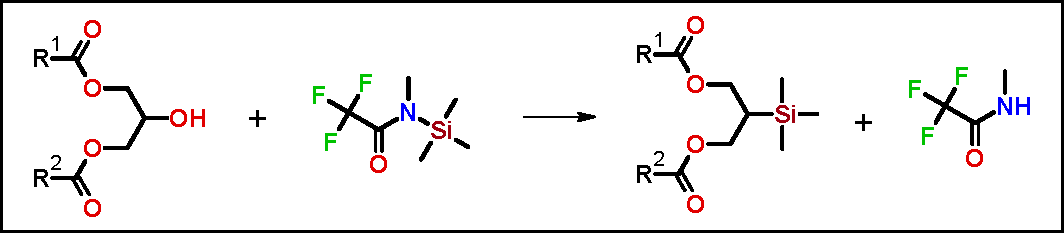
\includegraphics[width=\textwidth]{Figures/Derivitization.pdf}
\decoRule

\caption[Derivitization]{The derivitization of a diglyceride with
N-methyl-N-(trimethylsilyl)-trifluoroacetamide (MSTFA). During GC the inert
trimethylsilyl group does not interact with the stationary support,
and the volatile trifluoroacetamide elutes with the solvent front.}

\label{fig:MSTFA}
\end{figure}

The trifluoroacetamide group is a good leaving group, and upon nucleophilic
attack by the hydroxyl oxygen its bond with the trimethylsilyl (TMS) group is cleaved,
leaving the TMS bound to the oxygen. The labile hydrogen atom is now replaced by
the TMS group, which is inert and will not interact with polar entities in the
stationary phase or column, which will lead to improved peak shapes. 

\subsection{Free Glycerol}

Free glycerol is one of the products of the transesterification of plant oils to
produce biodiesel. It is a polar compound, which naturally separates from
non-polar biodiesel, and any excess remaining dissolved in the biodiesel is
removed during the washing step. Free glycerol contributes to injector coking. 

Inappropriate processing may leave excess free glycerol in the biodiesel, and
therefore determining free glycerol is an important quality-control step.

Free glycerol can be determined by the same chromatographic procedure prescribed
for the determination of the other glycerides in SANS 54105 (see Section
\ref{sec:Glycerides}, but SANS 1935 also offers the option of SANS 54016. This
standard uses a liquid-liquid extraction of biodiesel with a mixture of ethanol,
water, and hexane. The free glycerol transfers quantitatively to the bottom
layer, which is then analysed with a gas chromatographic method. The benefit of
this method is that the resulting chromatogram has only one peak, that of
glycerol, so quantification is straightforward.

The column specified in SANS 54106 method is a PLOT column, \textit{i.e.} a
Porous Layer Open Tubular column, which is a capillary lined on the inside with
a layer of particles coated with the stationary phase, in this case a polar
polyethylene glycol. 

\subsection{Polyunsaturated methyl esters}
\label{sec:ChromDetUnsat}

The degree of unsaturation of the constituent fatty acids is the main
determinant of the oxidative stability of biodiesel. SANS 1935 limits the amount
of highly unsaturated FAMEs by two lines in Table 1. In particular, the amount
of methyl linoleate is limited to less than \SI{12}{\percent} mass fraction, and
the amount of polyunsaturated fatty acid methyl esters with four or more double
bonds is limited to less than \SI{1}{\percent} mass fraction.

\subsubsection{Linolenic acid methyl ester}

The prescribed method for the determination of methyl linoleate (C18:3) is SANS
54103, the same method as prescribed for total esters (see Section
\ref{sec:EsterContent}).

\subsubsection{Highly unsaturated fatty acid methyl esters}

Polyunsatured fatty acids (PUFAs) with more than four double bonds are not
commonly found in plant oils, but are found in algae. Fish that feed on algae
accumulate these oils, so that they are also found in fish oils, but fish oil is
not a sustainable resource and should not be used for fuel
\autocite{Kitessa2014}. PUFAs are also highly oxidatively unstable, and
therefore undesirable in biodiesel.

The method prescribed for the determination of PUFA FAMEs is EN 15779. This
method uses a capillary column with a polyethylene glycol stationary phase.

\section{Comparison of SANS 1935 and SANS 342}

SANS 1935 sets the standard for neat biodiesel or biodiesel blendstock in South
Africa, and SANS 342 sets the standard for petrodiesel. As can be expected,
there is considerable overlap between the requirements of petrodiesel and
biodiesel, summarized in Figure \ref{fig:Venn}.

\begin{figure}
\centering
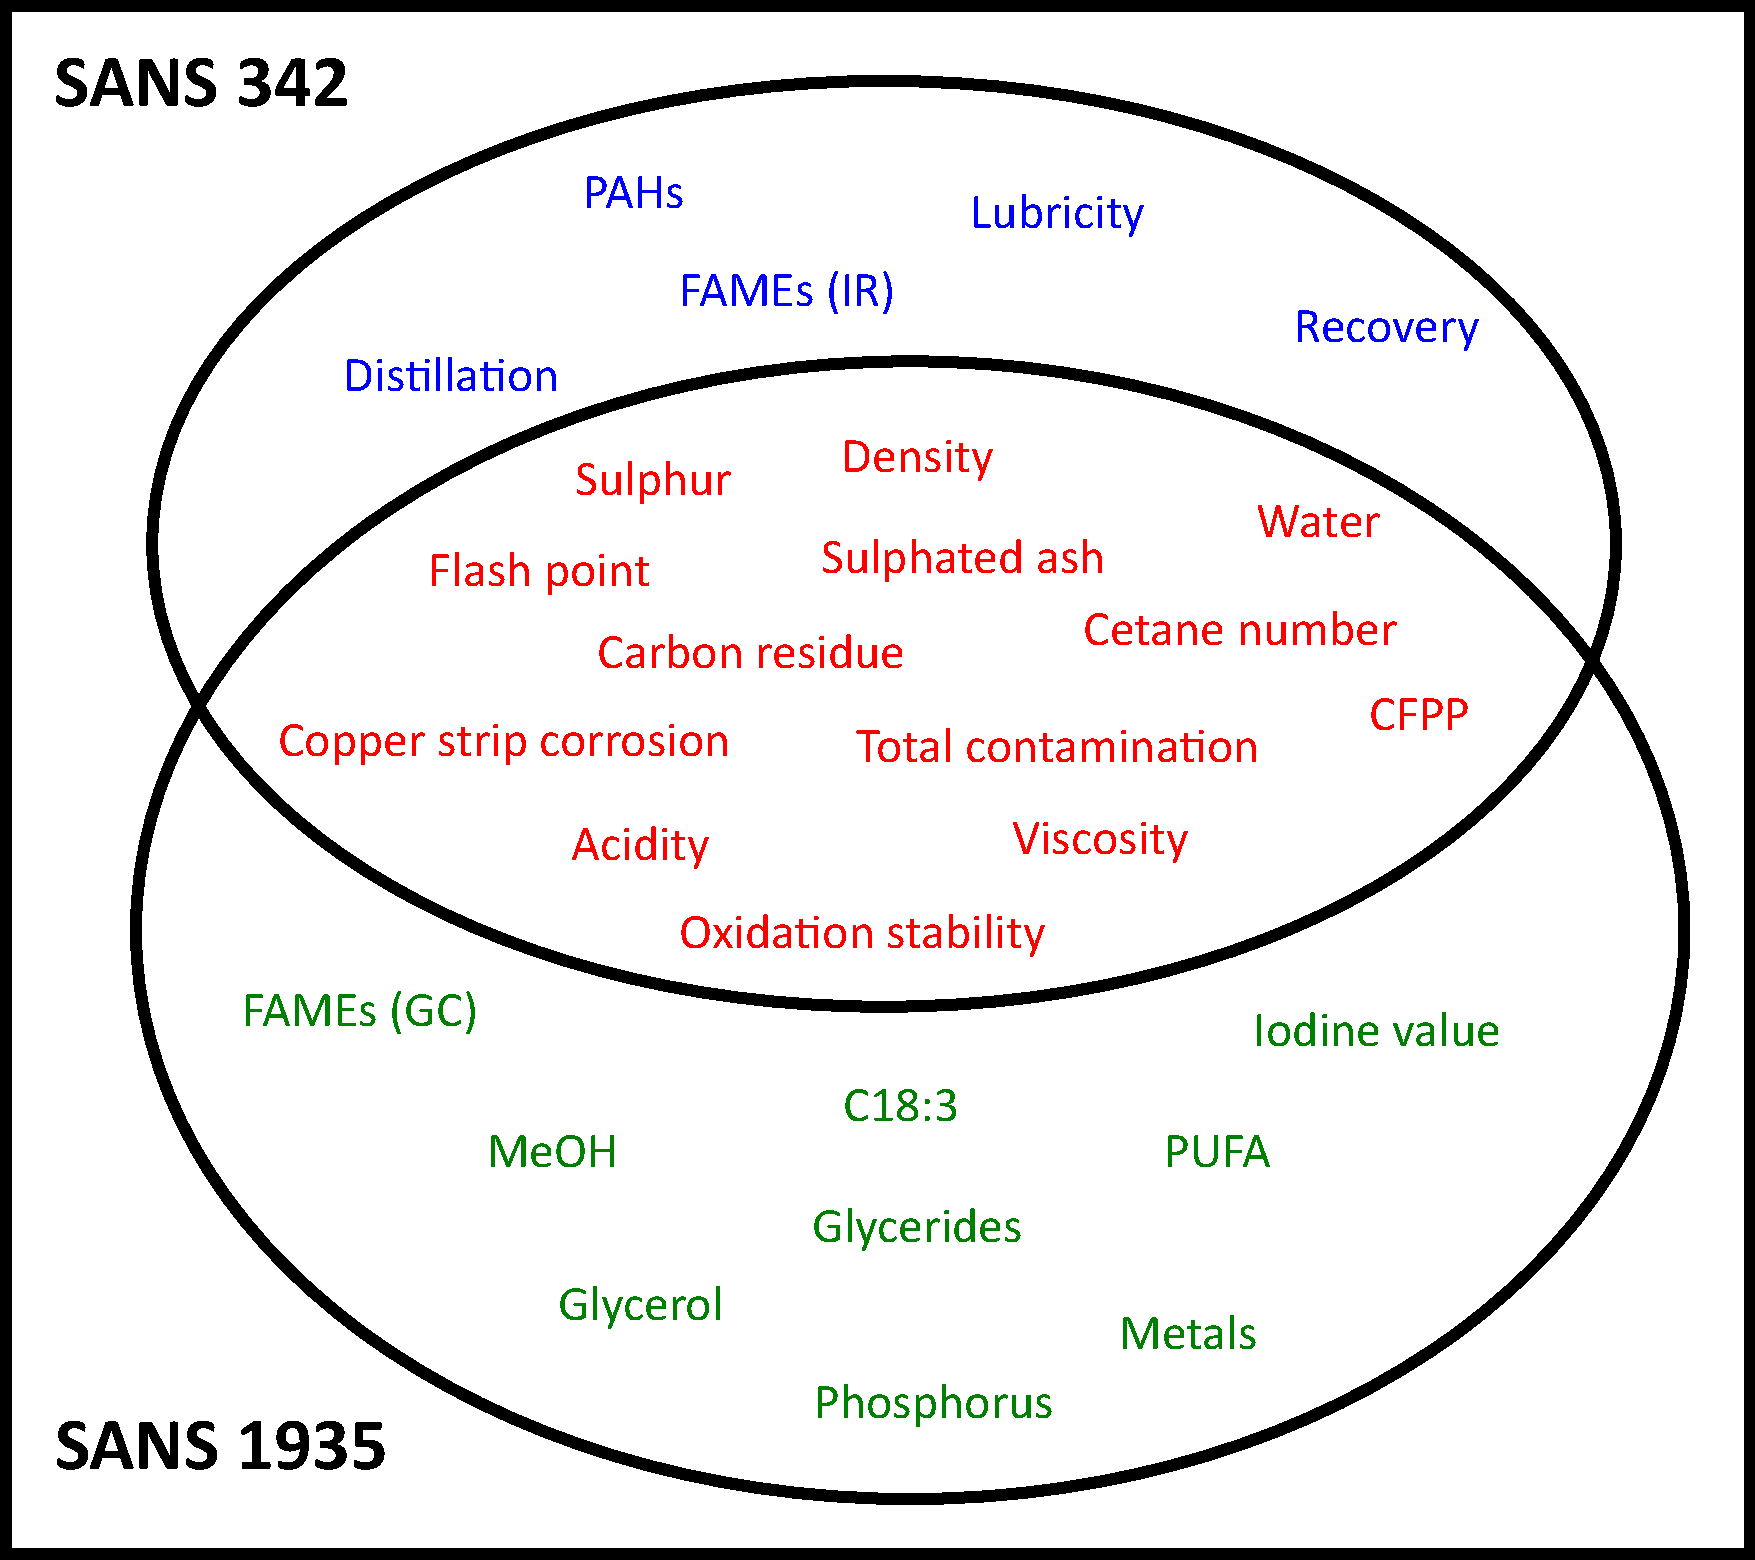
\includegraphics[width=\textwidth]{Figures/Venn.pdf}
\decoRule

\caption[Overlap of requirements ]{The overlap of requirements }

\label{fig:Venn}
\end{figure}

The amount of \keyword{Polycyclic aromatic hydrocarbons} (PAHs) in petrodiesel
is limited to help control their levels in the environment. PAHs have many
sources, including uncombusted petrodiesel.

The Petroleum Products Act allows the blending of up to \SI{5}{\percent} of
biodiesel with petrodiesel without the need to label it explicitly as a biodiesel
blend. The method prescribed by SANS 342 for determining the FAMEs in
petrodiesel is EN 14078. This is an infrared spectrophotometry method: the
amount of infrared radiation absorbed by a sample of diesel is compared to the
radiation absorbed by solutions containing known amounts of FAMEs. This method
is based on the strong absorption of the carbonyl group at
\SI{1745}{\per\centi\metre}. Petrodiesel exhibits low absorbance at this
wavelength, because petrodiesel contains carbonyl compounds only at trace
levels. Like all spectroscopic methods it suffers from spectral interference,
which can go unnoticed \autocite{Pinho2014}.

The pumps in modern diesel engines generate pressures of up to
\SI{2500}{\bar}, which imply that the mechanical parts exert large forces on each other.
Metal parts that transmit large forces need to be lubricated to limit wear to
acceptable rates. Some of these parts are immersed in the fuel, and can
therefore not be conventionally lubricated: the circulating fuel will rapidly
dissolve and sweep away any grease or lubricating oil. Therefore all the
lubrication depends on the lubricating properties of the fuel itself.
\keyword{Lubricity} is a measure of the lubricating properties of a fuel. It is
an aggregate property, and it is quantified by the \keyword{wear scar} caused
when two metal parts of specified shape are rubbed against each other with a
specified force for a specified duration. Such tests are done using
special-purpose test machines.

SANS 1935 contains no lubricity requirement, because it has been found that
biodiesel always provides adequate lubricity. Also, biodiesel can be used as a
lubricity improver in ultra-low-sulphur petrodiesel that might not meet the
requirement. This lubricity is not provided by the FAMEs, but by the polar
impurities in the biodiesel, such as free fatty acids and monoglycerides
\autocite{Knothe2005}.

\section{Conclusion: room for innovation.}

The diversity of chromatographic biodiesel quality control methods implies that the
compliance with SANS 1935 can be expensive. To comply, a biodiesel producer will
have to submit samples of biodiesel to at least four different kinds of
chromatographic analysis:

\begin{itemize}
  \item EN 14105 for free and total glycerol
  \item EN 14103 for FAME and methyl linoleate content
  \item EN 14110 for residual methanol 
  \item EN 15779 for highly unsaturated FAMEs
  \item (Optionally) EN 14106 for free glycerol
\end{itemize}

This might prove costly, and there has been at least one innovation to reduce
the number of instruments required \autocite{McCurry2009}.

As was emphasized in the introduction to this chapter (see Section
\ref{Sec:Intro}), standards are not `the best' way of determining a certain
desirable property of biodiesel, they are merely trusted methods. As improved
methods are developed and become trustworthy, they can be adopted as
alternatives. As far as biodiesel is concerned, it seems that there is ample
room for chromatographers to innovate and develop improved methods and
instrumentation. This was the motivation for selecting biodiesel as a practical
challenge for developing SFC×GC.



% Chapter 4it

\begin{savequote}[\quotewidth]
$pV \neq nRT$ 
\qauthor{The universal gas law does not apply to supercritical fluids}
\end{savequote}

\chapter{Instrumentation: Supercritical Fluid Chromatography} % Main chapter title

\label{Chapter4} % For referencing this chapter elsewhere, use \ref{Chapter4}

In this thesis the development of a comprehensively coupled (supercritical fluid
× gas) chromatograph and its application to the analysis of biodiesel is
discussed. The discussion on the experimental work divides naturally into two
parts: this chapter discusses the supercritical fluid chromatography (SFC) and
the next chapter discusses the gas chromatography (GC).

\section{SFC}

As discussed in Chapter \ref{Chapter2}, an SFC chromatograph consists of a
supply of mobile phase, a pump, a pressure control system, a modifier control
system, a column, a pressure relief system and a detector. These subsystems are
discussed below.

\section{Mobile phase}

As mobile phase we used carbon dioxide. The benefits of carbon dioxide as an
solvent and mobile phase is discussed in Chapter \ref{Chapter2}. We used
\SI{99.995}{\percent} pure carbon dioxide supplied by Air Products. Our
colleauges in industry also use food grade or technical grade carbon dioxide and
they have not reported any significant impurities.

As modifier we used LiChrosolv\textregistered methanol from Merck. This is an
`HPLC-grade' solvent, of which the purification is optimized for the removal of
UV-absorbing impurities. Using this grade of solvents is important when using
optical absorbance or fluorescence detectors, because lowering levels of
impurities improve limits of detection. It is quite likely that a less expensive
grade of modifier would also be suitable for our SFC, because we do not use an
optical detector.

\section{Pump}
\label{sec:CO2Pump}

As pump we used the robust, reliable Varian 8500 HPLC pump because it was
available. This pump had its control electronics removed, and it was controlled
from a personal computer by software written for the purpose. The Varian 8500
pump is driven by a stepper motor. This kind of motor turns in discrete steps,
instead of at a constant rate. It is driven by pulses of electric current,
rather than a continuous current, and therefore the speed of the motor can be
controlled by varying the rate of the pulses. This makes it relatively simple to
control the speed of the motor from a computer. The Varian 8500 pump has a
built-in pressure transducer that provides an electronic signal proportional to
the pressure at the pump outlet.

The Varian 8500 pump is a single-piston pump with a \SI{250}{\milli\litre}
capacity that needs to be refilled between strokes. Refilling means that one has
to stop chromatography, which makes it important to fill the pump to full
capacity, so that chromatographic runs are not interrupted. This means that the
pump needs to be filled with carbon dioxide in the liquid phase rather than the
vapour phase. Compressing either would create the appropriate phase for doing
chromatography, but compressing a vapour would leave one with a much smaller
volume of high-pressure carbon dioxide than compressing a liquid. Filling a pump
with liquid carbon dioxide is more difficult than one might imagine.

\begin{figure}
\centering
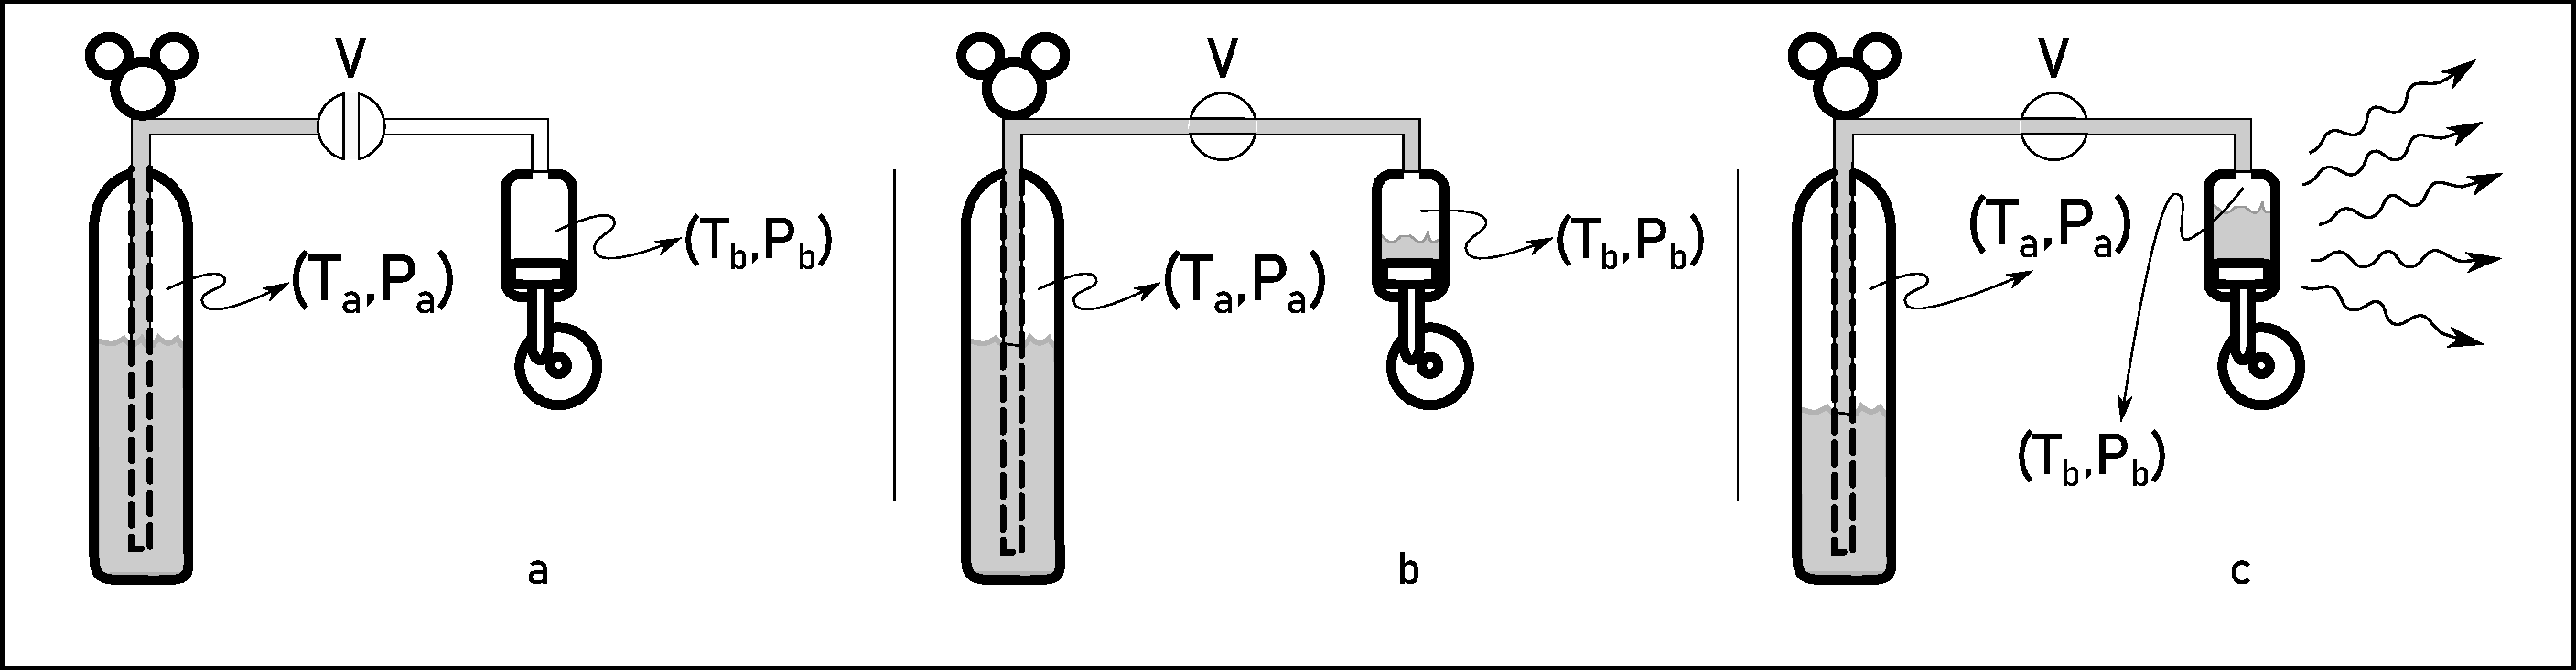
\includegraphics[width=\textwidth]{Figures/CO2Filling.pdf}
\decoRule

\caption[Fillng a CO\textsubscript{2} pump.]{A schematic diagram of the process of the filling of
the carbon dioxide pump. (a) The pressure in the reservoir $P_a$ is much higher
than the pressure in the receptacle $P_b$. The valve is closed, so there is no
flow. (b) The valve is open and some carbon dioxide has flowed from the
reservoir to the receptacle. But $P_b = P_a$, so there is no flow. (c) When the
temperature in the receptacle $T_b < T_a$, then $P_b  < P_a$, following
Gay-Lussac's law. Flow will continue until all the vapour in the receptacle has
condensed.}

\label{fig:co2fill}
\end{figure}


Imagine a reservoir of liquid carbon dioxide, equipped with a dip tube,
connected to an empty receptacle via a valve (V). (See Figure \ref{fig:co2fill})
One can assume that the receptacle is empty and contains only carbon dioxide
vapour at atmospheric pressure, say \SI{1}{\bar}. The vapour pressure of the
vapour above the liquid in the reservoir is about \SI{55.3}{\bar} (5.6 MPa).
When the valve (V) is opened the will high-pressure vapour in the reservoir will
expel the liquid carbon dioxide through the dip tube and through the valve, into
the receptacle. In the low-pressure environment of the receptacle the carbon
dioxide will boil. Soon there will be some liquid carbon dioxide in the
receptacle, with the rest of the receptacle volume filled with gaseous carbon
dioxide. When the system comes to equilibrium the pressure in the receptacle
($P_b$) will equal the pressure in the reservoir ($P_a$), and there will be no
flow of liquid carbon dioxide. One can attempt to now increase the flow by
increasing the volume of the receptacle (for example by withdrawing a pump
piston), and hence decreasing the vapour pressure there. But any flow from the
reservoir will lead to expansion of the headspace of the reservoir. This will
lead to cooling of the vapour, and therefore lower pressure and therefore lower
flow. The final result of this process is that the receptacle is never filled to
capacity with liquid.

The only way to restore the flow from the reservoir to the receptacle is to
create a pressure difference $P_a - P_b$. While it is possible to create an
overpressure in the reservoir by adding a headspace gas, it is technically
challenging and expensive. It is simpler to use the Gay-Lussac gas law.
According to this law the ratio of the pressure to the temperature of a gas is
constant so that $\frac{P_b}{T_b} = k$. This means that a decrease in
temperature will lead to a decrease in pressure. The way to fill the reservoir
to capacity is to ensure that the temperature of headspace vapour $T_a$ is higher
than the temperature of the headspace vapour $T_b$. Because safety regulations
prohibit the heating of a cylinder of pressurized gas, the way to ensure $T_a <
T_b$ is to cool the receptacle. This cools the headspace vapour, and following
the Gay-Lussac law the pressure $P_b$ decreases, the difference $P_a - P_b$
increases and the liquid flows until the receptacle is filled to capacity.
 
In the case of the Varian 8500 pump the cooling of the pump was achieved by
wrapping a coil of copper tubing around the cylinder, and pumping a chilled
heat-exchange fluid through it. A chiller with a mechanically cooled tank with a
\SI{20}{\litre} capacity was filled with a solution of \SI{5.0}{\litre} of
diethyl glycerol in about \SI{10}{\litre} of water. This mixture has a freezing
point of \SI{-15}{\celsius}, which can be cooled by the chiller without
freezing. (If the coolant freezes a layer of ice forms on the cooling plate of
the chiller, which isolates the remaining liquid from the cooling plate and
limits the minimum temperature of the coolant.) An inexpensive submersible water
pump (designed for decorative water fountains) was used to pump the coolant
through the circuit. This pump can deliver \SI{800}{\litre} of water per hour at
a head of \SI{1.2}{\metre}.

For some experiments we also used a SFT-10 pump from Supercritical Fluid
Technologies (Newark, Delaware). This is a purpose-built two-piston pump with
sapphire valve seats and a Peltier-cooled head. This is a much better technology
than the HPLC pumps. It takes up less space and does not need refilling, since
it feeds directly from the cylinder. This pump had its own microprocessor
controllers on board, and flow and pressure could simply be commanded from the
PC through a USB cable.

\subsection{Pressure control system}

The aim of chromatography is to separate chromatograms by a certain distance.
But the days of separating coloured compounds in glass packed columns are long
past and the direct measurement of distances are now relegated to thin-layer
chromatography. Instead, we have to make do with proxies for distance such as
\keyword{retention volumes} or \keyword{retention times}.


% In chromatography the figure of merit by which the performance of a system is
% measured is the distance by which two compounds are separated, relative to their peak
% widths. This is known as the \textit{resolution}. 

Retention times are particularly convenient today, because they can easily be
measured by computer systems. Retention times, however, depend on a known flow
rate of the mobile phase through the column. The flow rate need not be constant,
although for the sake of simplicity a constant flow rate is preferred. Ideally,
the flow rate should also be adjustable. The need for an adjustable, constant
flow rate can be met by using a control system. Control systems are well
understood by engineers, among whom it is a major field of study
\autocite{Koenig2009}.

Figure \ref{fig:processcontrol} shows a diagram of a simple process control
system. Some aspect of the process under control is measured, which yields the
\keyword{process variable} (PV). The PV is compared to the \keyword{set value}
(SV), and the \keyword{error} (e) is obtained by finding the difference. The error
is provided to the controller, which calculates the \keyword{manipulated
variable} (MV). The MV is used to drive the final control element, which adjusts
the process with the aim of producing a smaller error.

\begin{figure}
\centering
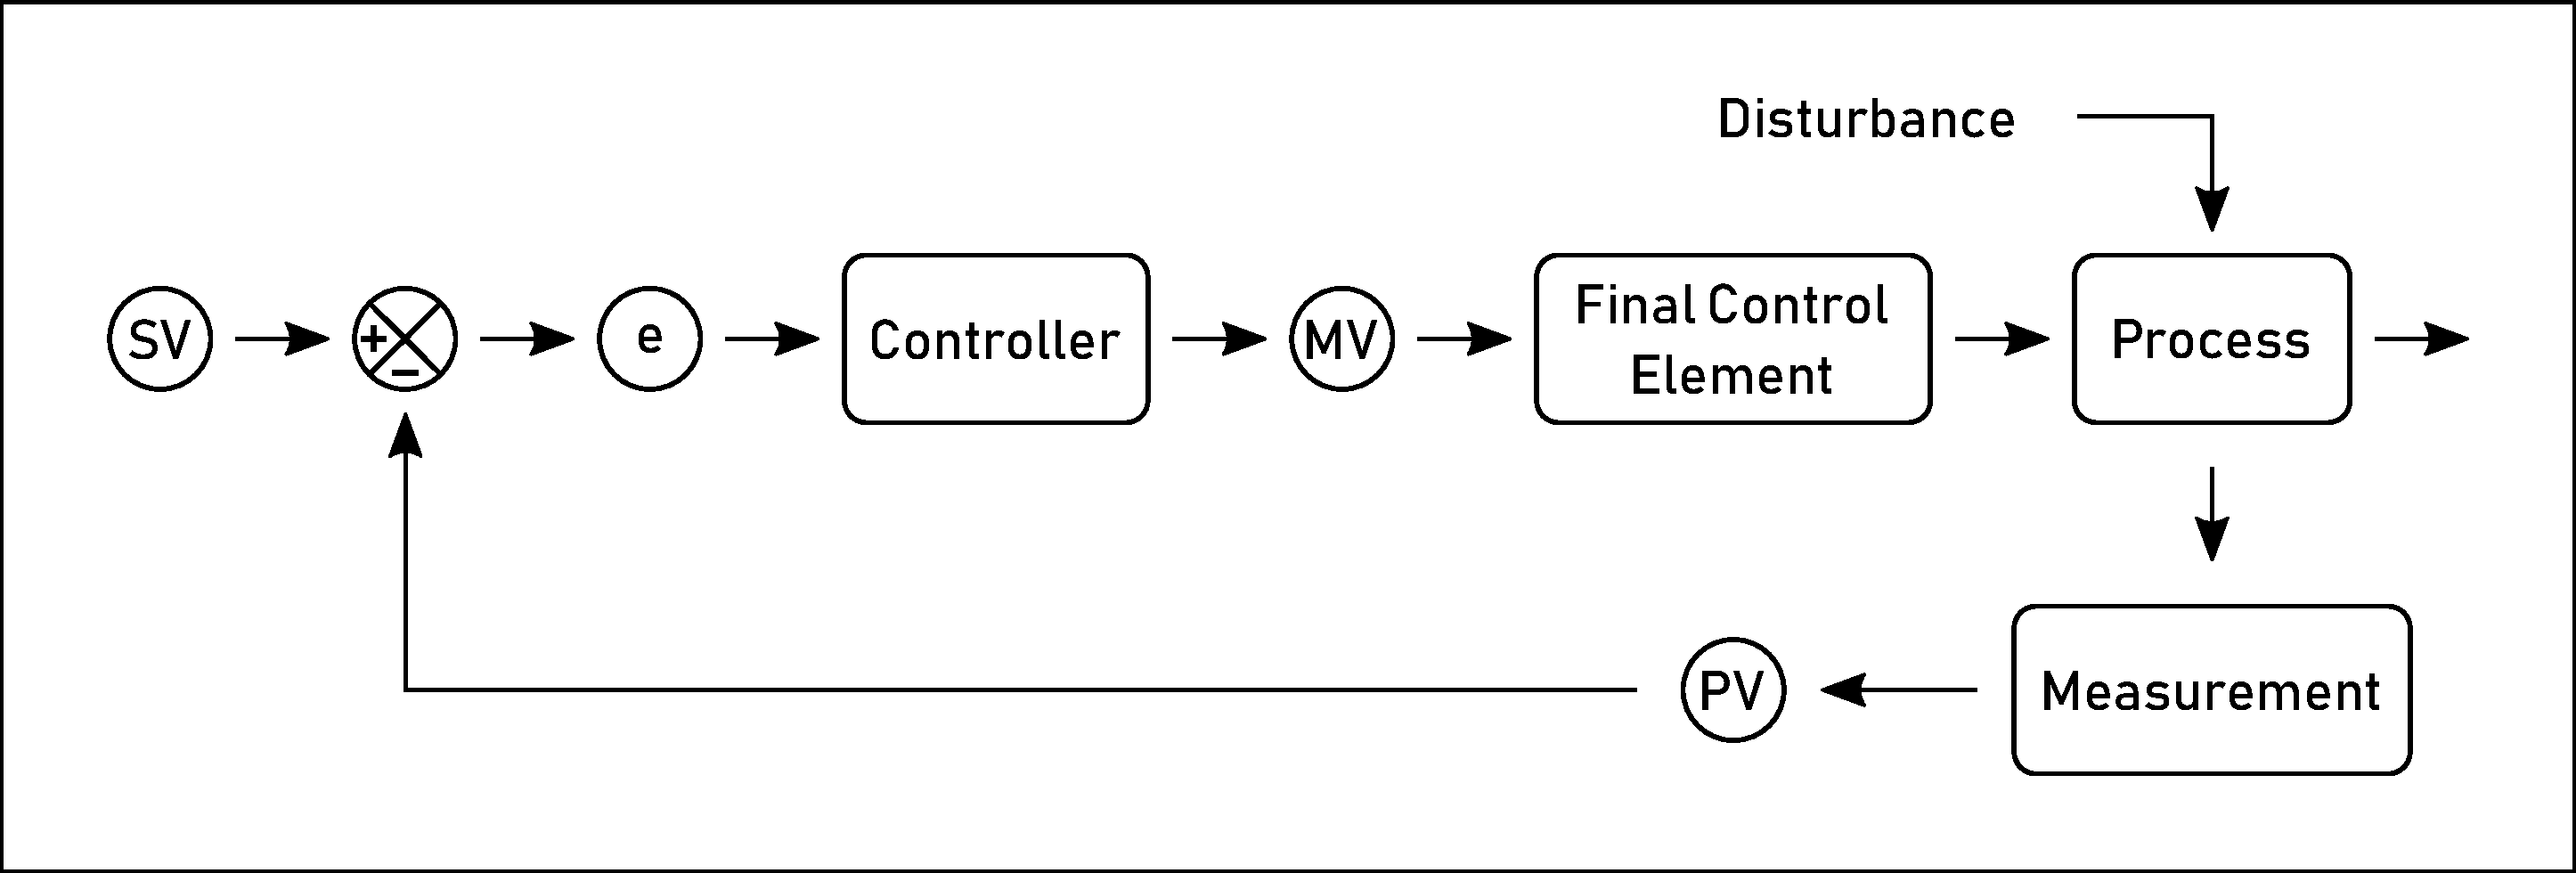
\includegraphics[width=\textwidth]{Figures/ProcessControl.pdf}
\decoRule

\caption[A process control system]{Schematic diagram of a closed-loop control
system. (SV) Set Value, (PV) Process Variable, (e) Error, (MV) Manipulated
Variable}

\label{fig:processcontrol}
\end{figure}

Chromatographic systems conventionally work under pressure control or flow
control regimes. Either is suitable: constant pressure systems usually yield
constant flow if other parameters are held constant. Because flow measurement is
more complex than pressure measurement, pressure control is the older, simpler
and less expensive control method. Also, in SFC the solvent strength of the mobile
phase is pressure/density dependent. We therefore selected pressure control
as our control regime.

In our system the pressure measured by the on-pump sensor was the process
variable (PV) . This was compared to the set value (SV) set on the computer
console. The controller was a software algorithm, implemented as a virtual
instrument in the programming environment LabVIEW. The controller computed an
output value for the manipulated variable (MV), which was the rate at which
pulses were sent to the pump, in hertz. The digital input/output (DIO) interface
of a National Instruments PCI-6014 multifunction data acquisition board created
those pulses and sent them to the pump's electronic interface.

The software used a PID (Proportional-Integral-Derivative) controller module,
with the Integral and Derivative contributions disabled. The simpler
proportional control was found totally adequate for our purpose, and it can be
improved in future by finding an appropriate tuning method and applying it with
the integral and/or derivative activated.

% While enabling the Integral and Derivative contributions would add to the
% accuracy of the controller, we could not find a suitable, simple tuning
% procedure.

% Tuning the controller from adequate performance to optimum performance would
% consume resources while not improving the chromatography.

\subsection{Modifier Control}

The modifier needs to be present in the mobile phase at a known and controlled
concentration. There are various SFC-modifier mobile phase supply units on the
market. They tend to be expensive and complex, because they require the use of
two controlled, high-pressure pumps. Given that our needs were rather modest, we
elected to use a simpler system. Instead of accurately pumping the supercritical
fluid and the modifier, we only pump and control the supercritical carbon
dioxide and add measured volumes of modifier.

The modifier control unit consisted of a six-port valve, a fixed-volume
measuring loop, and a mixing chamber. The unit operates by filling the measuring
loop with modifier, and then switching the measuring loop into the flowing
mobile phase. The modifier is washed into the mixing chamber, where it is
intimately mixed with and dissolved in the supercritical carbon dioxide. The
concentration of modifier in the mobile phase is determined by the switching
rate of the sampling valve. Given that about 3 volumes of supercritical carbon
dioxide is needed to wash the modifier out of the loop, the highest
concentration of modifier that can be added in this manner is about
\SI{25}{\percent}.

Figure \ref{fig:mixingchamber} shows the chosen design of the mixing chamber.
The inlet and outlet pipes of the mixing chamber extend far into the chamber, to
break up plug flow and encourage rapid mixing.  

\begin{figure}
\centering
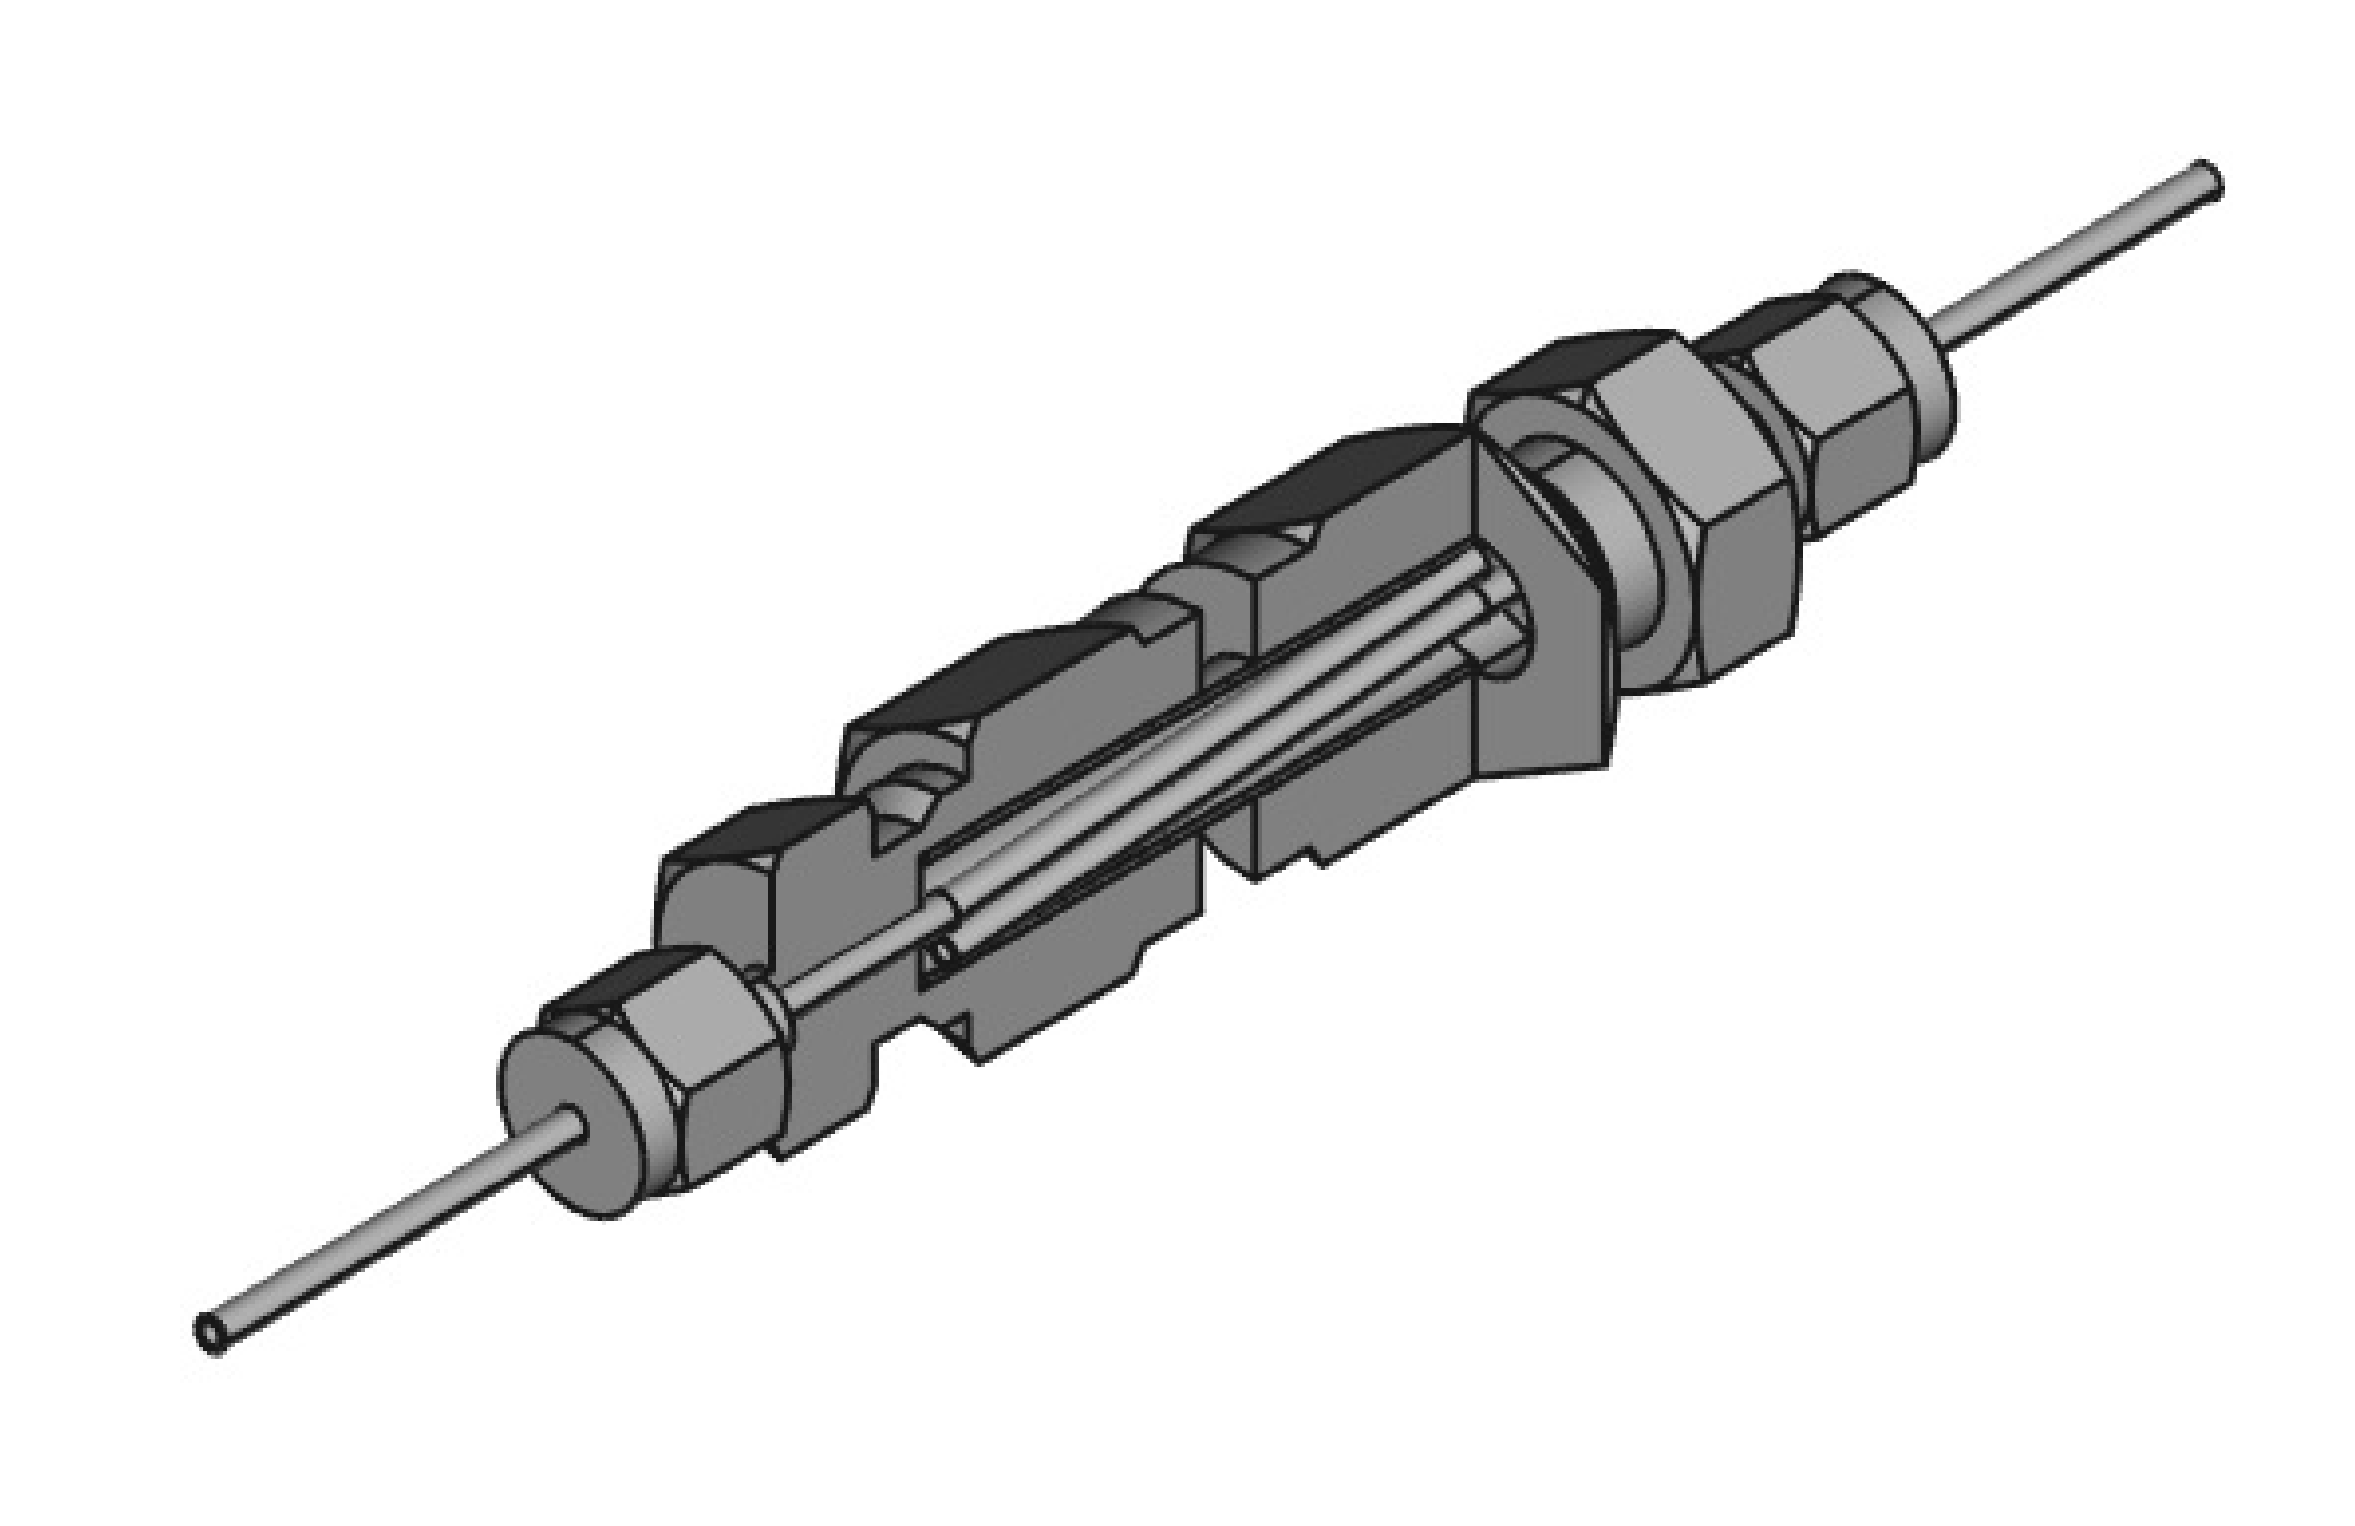
\includegraphics[width=\textwidth]{Figures/MixingChamber.png}
\decoRule

\caption[A cutaway diagram of the mixing chamber]{A cutaway diagram of the
mixing chamber design. The chamber is designed for the mixing of the modifier
and the supercritical carbon dioxide.}

\label{fig:mixingchamber}
\end{figure}

The modifier injection valve position was commanded from the controlling PC by electronic
voltage pulses.

\section{Sample injection}
\label{sec:SFCInjection}

The sample inlet was a two-position rotary valve with an internal sampling
volume (Figure \ref{fig:samplingvalve}). In one position the sampling volume is
filled with a syringe, and when the valve was commanded to inject the sampling
volume is switched into the carrier mobile stream. The sample volume was
\SI{0.5}{\micro\litre}. The injection valve position was commanded from the
controlling PC by electronic voltage pulses.

\begin{figure}
\centering
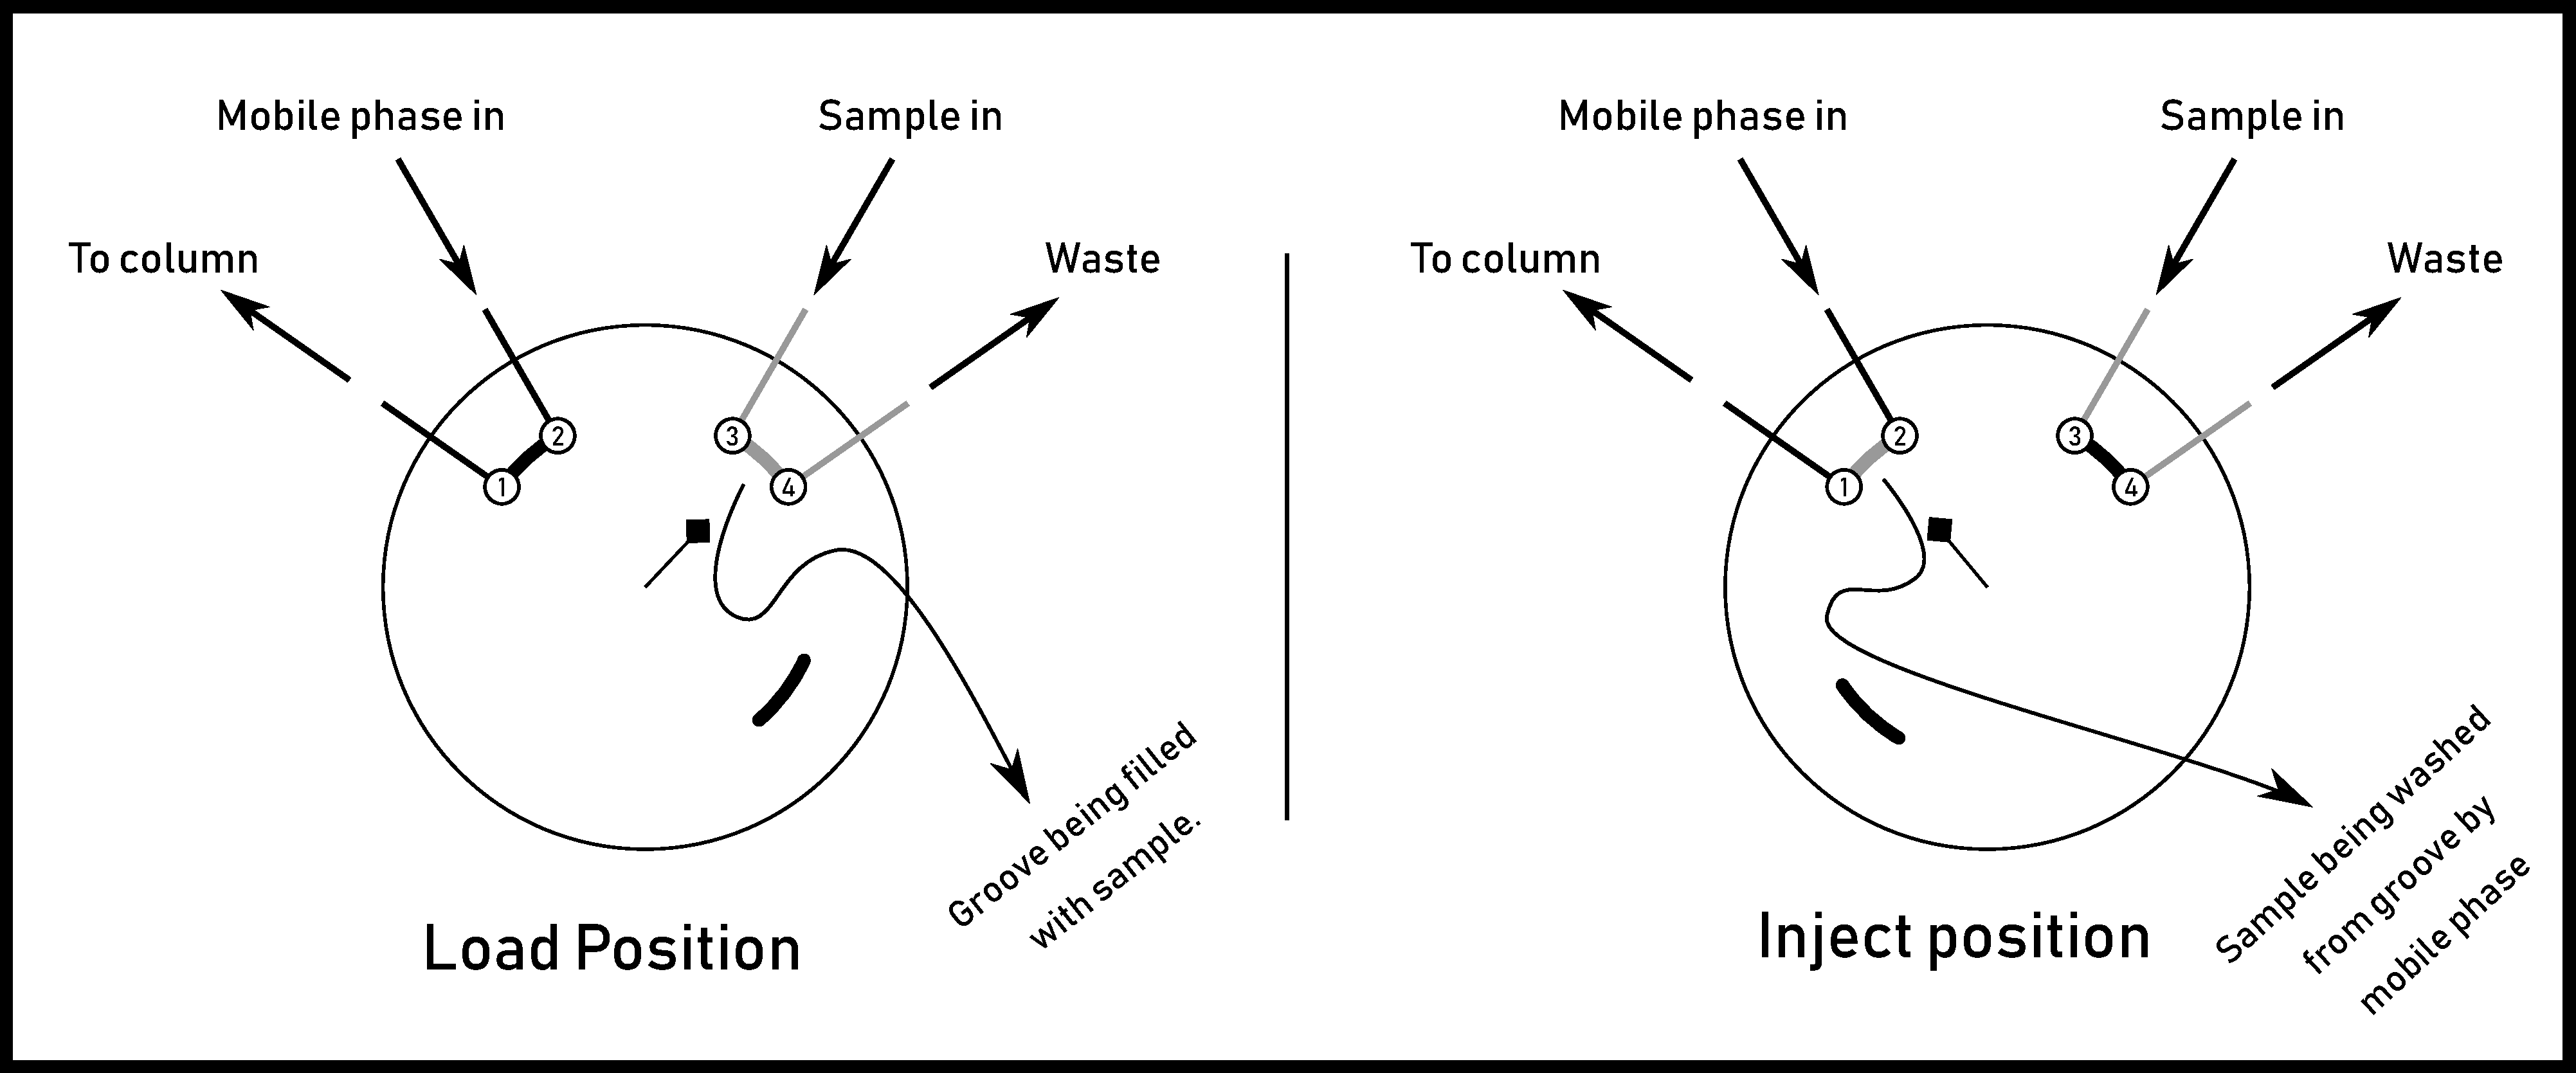
\includegraphics[width=\textwidth]{Figures/SampleValve.pdf}
\decoRule

\caption[Schematic diagram of the injection valve.]{A schematic diagram of the sampling valve. }

\label{fig:samplingvalve}
\end{figure}

The reader might be more familiar with the six-port valve as an injection
system. The benefit of the internal groove injection valve is that it allows a
much smaller volume to be injected. Using this small volume makes it possible to
inject samples without dilution, which simplifies sample preparation. A drawback
of this design is that it is not possible to vary the volume of sample injected.


\subsection{Column}
\label{sec:SFCColumn}

The separation power of a chromatographic system can be modelled by the equation 

\[
 R_s = \left(\frac{\sqrt{N}}{4}\right)  \left(\frac{\alpha-1}{\alpha}\right)  \left(\frac{k'}{1+k'}\right)
\]

were \(R_s\) is the \keyword{peak resolution}, \(N\) is the \keyword{number of
plates}, \(alpha\) is the \keyword{selectivity}, and \(k'\) is the
\keyword{retention factor}.
 
The number of plates \(N\) can be increased simply by making the column longer,
at the cost of increasing the time of the run. The maximum length of the column
is determined by the pressure drop available that will still yield adequate
flow. In capillary gas chromatography the openness of the column and the low
viscosity of the gas-phase mobile phase routinely allows columns \SI{100}{\metre
}long at inlet pressures of a few atmospheres. In HPLC the high viscosity of the
mobile phase and the narrow, tortuous pathways between the small particles of
the packing material means that the columns are typically
\SIrange{100}{200}{\milli\metre} long, requiring hundreds of atmospheres of
inlet pressure for adequate flow.

The low viscosity of an SFC mobile phase allows operation of much longer
HPLC-type packed columns. This provides a much higher number of plates in the
chromatographic system than HPLC. The SFC column we used in the SFC×GC system
was a set of five HPLC columns (\SI{150}{\milli\metre} $\times$
\SI{4.6}{\milli\metre}, \SI{3}{\micro\metre} particles) (Restek, Pinnacle DB
Silica) connected in series.

The stationary phase in this column is `bare silica', which is usually
considered 'polar'. That means that the packing of the column consists of porous
silica particles with no organic phase covering its surface, and hence one that
will interact strongly with polar molecules. In contrast, the ubiquitous `C18'
stationary phase used in reverse-phase HPLC is 'non-polar'. The particles of
such a stationary phase are coated with octadecyl chains bonded to its surface,
and hence will tend to interact strongly with non-polar molecules. The base
material of the particles is usually silica, but that is only because
manufacturing uniform particles of a given size from silica is a mature
technology and not because silica is important to the separation mechanism. (In
fact, some care has to be taken to deactivate the silica so that it does not
contribute to the retention. Such a mixed retention mechanism can lead to
\keyword{peak tailing}.)

\subsection{Stopped-flow}
\label{sec:stopflow}

Among analytical chemists it is the convention that chromatographic runs are
done without interruptions. In our SFC×GC chromatograph we collect fractions of
SFC eluate and separate them by GC. It is possible to collect, store and inject
fractions of SFC eluate while maintaining continuous flow, for example using a
dual storage loop system like the one depicted in Figure
\ref{fig:continuousflow}. But such systems require careful selection of volumes,
fraction collection reservoirs with matching volumes, and an auxiliary pump.

\begin{figure}
\centering
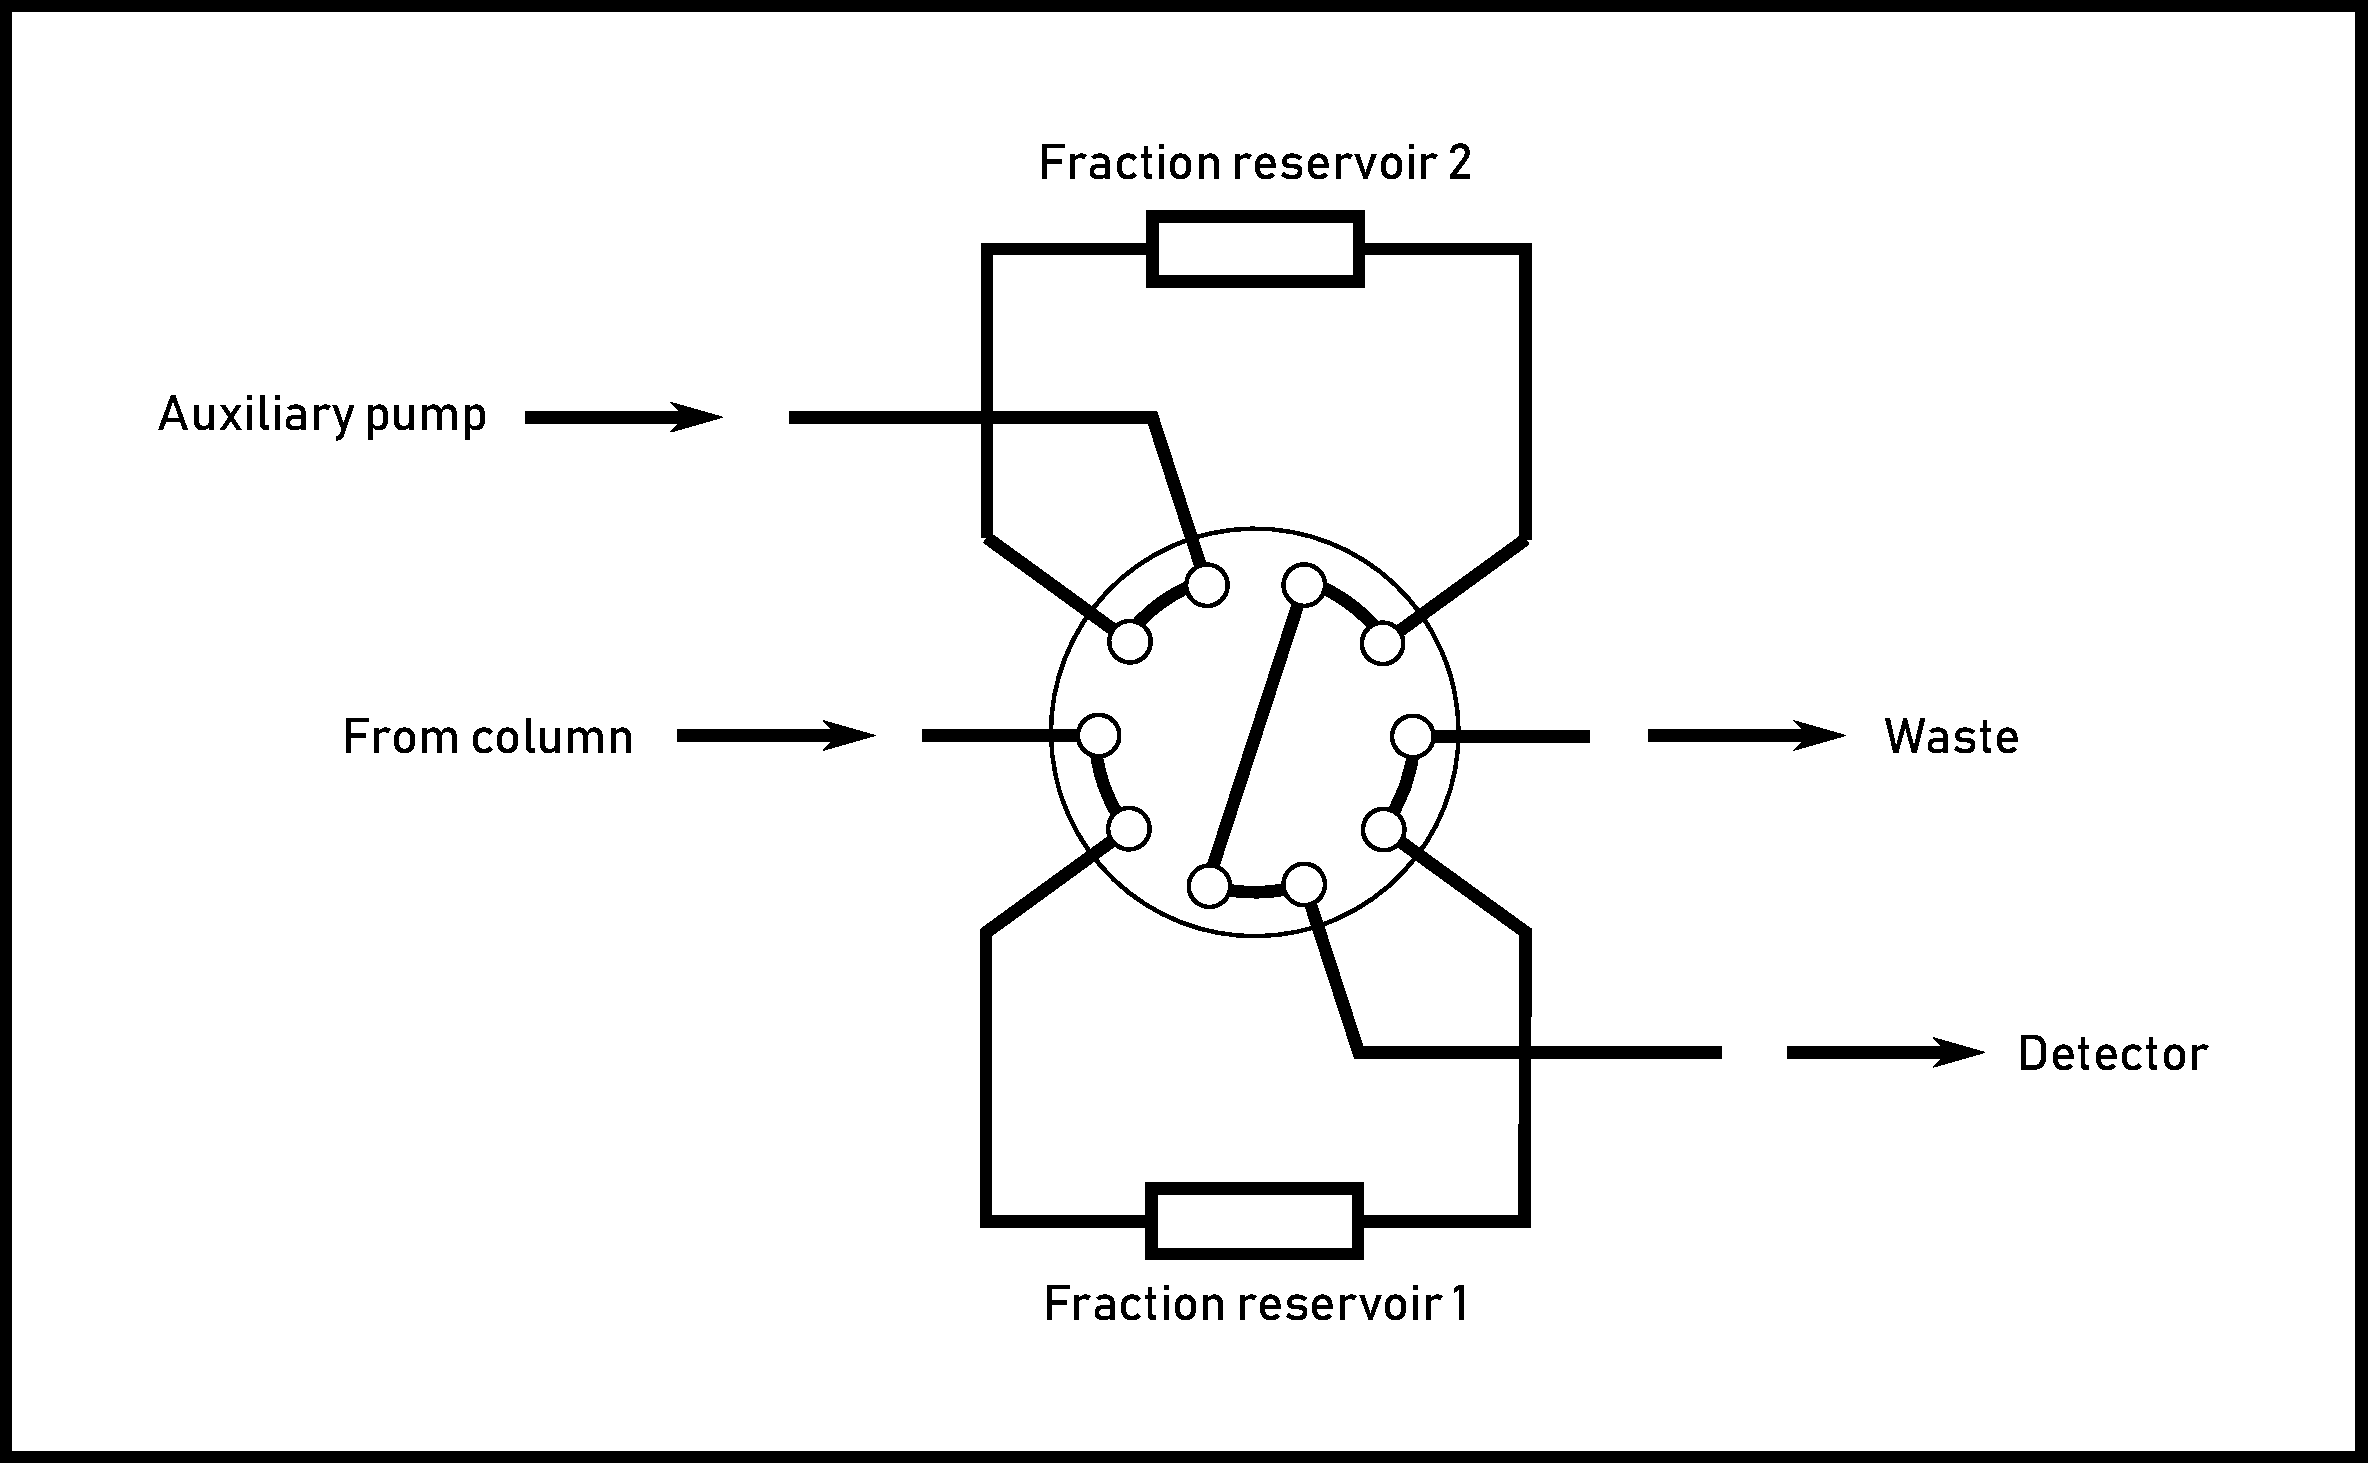
\includegraphics[width=\textwidth]{Figures/ContinuousFlowStopValve.pdf}
\decoRule

\caption[Schematic diagram of a continuous-flow valve.]{A schematic diagram of a
valve configured to allow continuous-flow fraction collection. }

\label{fig:continuousflow}
\end{figure}

Instead of such a system, we opted for a more versatile and simpler stopped-flow
system. In this system a fraction of the SFC eluate is collected, and then the
flow through the column is stopped. While the flow is stopped the collected
fraction is subjected to separation by GC. The flow was stopped by a six-port
rotary valve using three of the ports, directing flow either to a blocked-off
port or to the depressurizer, in effect making it an on-off controller.

In packed columns, "eddy diffusion is always the main cause for peak broadening
at any temperature and at high velocities" \autocite{Gritti2006}. During the
period that the flow is stopped only longitudinal diffusion contributes to peak
broadening, which is small compared to eddy diffusion in dense mobile phases.
Using the simple stopped-flow technique of sample collection will therefore not
have a major effect on the resolution of the \oneD chromatography.


\section{Pressure Relief}
\label{sec:Restrictor}

No matter the kind of SFC system one uses, at some point the eluate needs to be
depressurized. This can be before or after the detector. If depressurization
happens after the detector, then the details of the mechanism doesn't matter
much, because the information has been obtained and the eluate can be discarded.
If, as in our case, the depressurized eluate needs to still pass the detector,
it is important to not lose the resolution achieved by the column.
This means that the design of the depressurizer requires some care.

The main concern in depressurizer design is premature desolvation of analytes.
This causes \keyword{discrimination}, which is the differential treatment of
substances where identical treatments are required. In particular, compounds of
higher molecular weight tend to desolve first from the supercritical fluid, and
might precipitate in the wrong place if the depressurizer is not designed to
prevent it. 

Depressurization can be done either statically or dynamically. In a dynamic
system there is an active element that controls the flow of the eluate in such a
way as to maintain the pressure upstream of the active element of the
controller. Such a device is often called a \keyword{back pressure regulator},
and is usually an electromechanical device with digital control. They tend to
be complex and expensive.

In static depressurization there is no active pressure control. A simple
\keyword{restrictor} is used to limit the flow between the high pressure of the
SFC and the low-pressure outlet. Textbooks often discuss different restrictor
designs. \autocite[The book by][provides an example.]{LuquedeCastro1994}. Our
preferred depressurizer was the `integral' or Guthrie design
\autocite{Guthrie1986}. Figure \ref{fig:restrictor} shows the steps in
manufacturing the Guthrie restrictor.

\begin{figure}
\centering
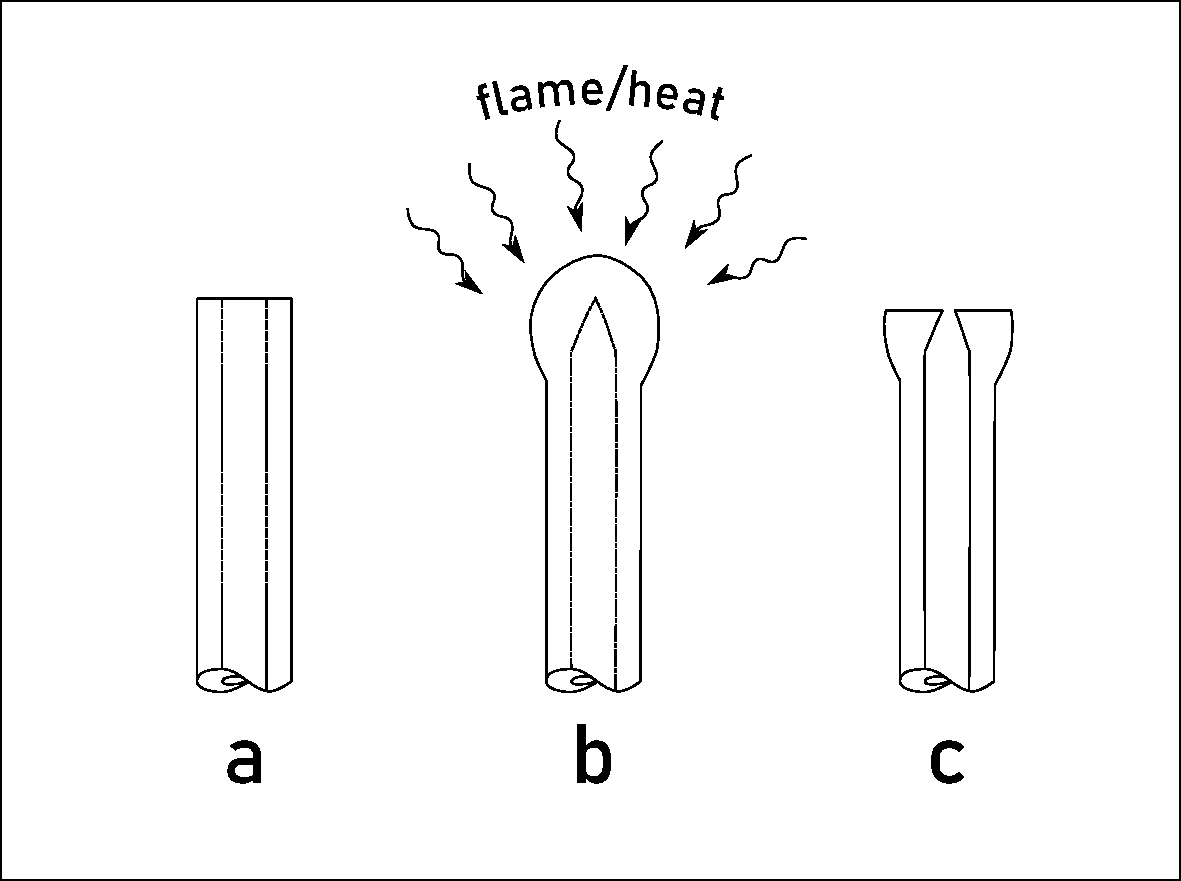
\includegraphics[width=0.5\textwidth]{Figures/Restrictor.pdf}
\decoRule

\caption[A diagram of a integral restrictor.]{The steps of making a Guthrie restrictor. (a) Cut
length of quartz capillary (b) Heat with flame to soften glass and create
internal cone (c) Grind down end to expose orifice of the appropriate size.}

\label{fig:restrictor}
\end{figure}

We found this restrictor robust and fairly simple to manufacture. It was
possible to adjust the flow to a given flow rate. This design of restrictor
should eliminate discrimination, because the decompression takes place in a very
short space.

However, the Guthrie design proved prone to blockage. These blockages could not
be eliminated by incorporating a \SI{0.5}{\micro\metre} filter before the
restrictor, which prompted an investigation into the cause of blockages. To rule
out the possibility that it was particles that caused the Guthrie restrictor to
become blocked, we first had to determine the diameter of the orifice. This
proved to be harder than expected: optical microscopy was not able to give a
simple, unambiguous measure of the orifice diameter. Scanning electron
microscopy (SEM) showed that the orifice diameter of a Guthrie restrictor is
about \SI{10}{\micro\meter}, as shown in Figure \ref{fig:restrictororifice} This
makes it very unlikely that particles with an origin in the SFC system blocked
the restrictor: even the \SI{3}{\micro\meter} particles from the column packing
material should not block this restrictor.

\begin{figure}
\centering
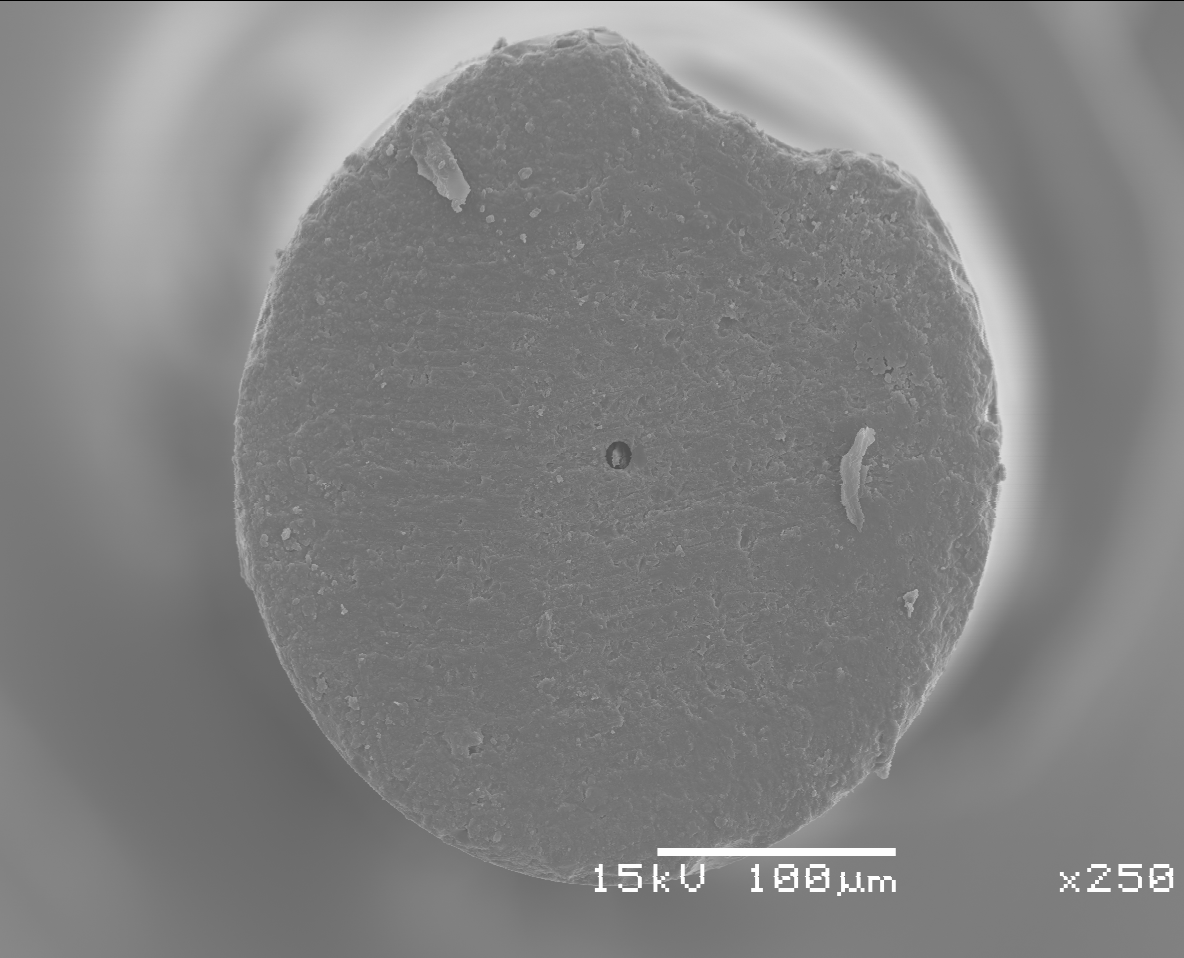
\includegraphics[width=\textwidth]{Figures/sem_h_001.png}
\decoRule

\caption[A electron microscope photo of a restrictor orifice]{An electron
micrograph of a restrictor tip, showing the size of the orifice.}

\label{fig:restrictororifice}
\end{figure}

Experience had taught us that the restrictor did not block if the flow was
continuous. It was only when the pressure in the restrictor cycled that
blockages occurred. To eliminate the possibility that it was material from the
stop valve (see Section \ref{sec:stopflow}) that caused the blockages, we cycled
the pressure by switching the pump on and off, allowing the pressure to bleed
off through the restrictor. This way of cycling the pressure did not prevent
blockages.

Examining the blocked restrictors with an electron microscope revealed that the
restrictors became blocked by a soft material. Backscatter SEM mode allows the
energy of X-rays to be measured by energy-dispersive spectrometry, which yields
information about elemental composition. While much care must be taken before
this information can be used for quantitation, it revealed that the deposited
material contains significant quantities of carbon and oxygen, and possibly some
chlorine. This points to the probability that the material blocking the column
is organic in nature, and possibly polymeric. See Figure
\ref{fig:restrictorblockage}.

\begin{figure}
\centering
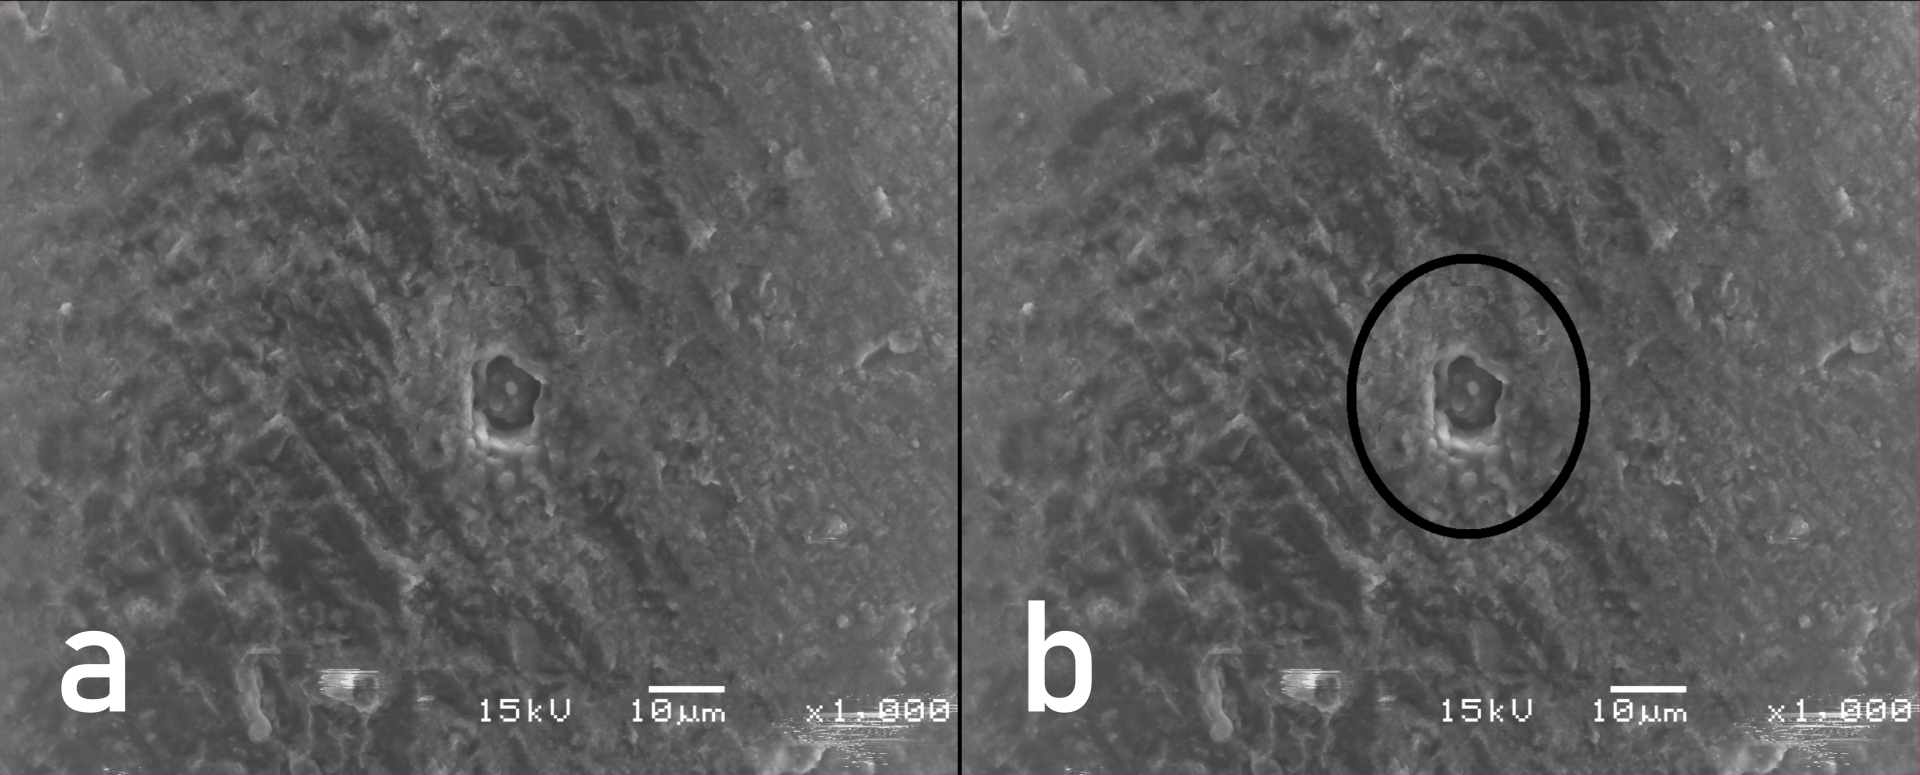
\includegraphics[width=\textwidth]{Figures/Blockage_1920.png}
\decoRule

\caption[A electron microscope photo of a blocked restrictor orifice]{An
electron micrograph of a blocked restrictor orifice. (a) Original
image (b) Image with black circle showing estimated original orifice location}

\label{fig:restrictorblockage}
\end{figure}

We could not determine the origin of the material, but it seems likely to be the
column, because cycling the pressure without a column did not cause a blockage.
We eliminated the possibility of blockage by sample material by using a brand
new column. We suspect that the blocking material might be remnants of
surfactants used in the synthesis of the silica gel stationary phase. These
surfactants are leached out of the column packing by the highly diffusive
supercritical fluid mobile phase, and they then precipitate in the restrictor
when the pressure drops and the compounds desolvate. Repetitive pressure cycles
causes a build-up of material which gradually blocks the orifice.

The smallness of the orifice contributes to the plugging problem. With a
diameter of \SI{50}{\micro\metre}, a solid sphere that fits in this capillary
will have a volume of \SI{0.065}{\nano\litre}, or \SI{65}{\pico\litre}. This
means that nanogram quantities of material can easily block the restrictor.

Being satisfied that an unfortunate combination of restrictor design and column
packing was the likely cause of the blockages, we chose a different restrictor
design. The choice was a simple linear restrictor and we trusted that heating
the end of the restrictor would prevent discrimination. The final linear
restrictor was \SI{800}{\milli\metre} long and had an internal diameter of
\SI{0.050}{\milli\metre}.

\section{Detector}

When SFC was first developed, a capillary column was the usual column, and an
FID was the usual detector. In current use, however, packed columns used with
mobile phase modifiers predominate and flame detectors have lost their place:
the high concentration of modifiers in the mobile phase would swamp the signal
from analytes or saturate the detector. Therefore modern SFC uses predominantly
UV/Vis optical detectors.

In the supercritical fluid chromatograph described in this chapter there was no
dedicated detector: the role of the detector was taken by a gas chromatograph.
This gas chromatograph collected fractions from the SFC, and separated them in
fast chromatographic runs with an FID detector, yielding comprehensive 2D
chromatograms. This chromatograph-as-a-detector is described in Chapter
\ref{Chapter5}.
 
% Chapter 5

\begin{savequote}[\quotewidth] There are no significant technical limitations to column
temperature programming in the order of a few hundred degrees per minute and
equally rapid cool-down rates.
\qauthor{Wolfgang Bertsch, 1997}
\end{savequote}

\chapter[Instrumentation: Fast GC]{Instrumentation: Fast temperature programmed gas chromatography} % Main chapter title

\label{Chapter5} % For referencing this chapter elsewhere, use \ref{Chapter5}

The topic of this thesis is the development of a comprehensively coupled
(supercritical fluid × gas) chromatograph and its application to the analysis of
biodiesel. The discussion on the experimental work divides naturally into two
parts: the topic of the previous chapter is supercritical fluid chromatography
(SFC) and of this chapter it is gas chromatography (GC).

\section{Speed of analysis}

The coupling between two chromatographs can be called \keyword{comprehensive} if
it meets the following criteria (as discussed in Section \ref{sec:SFCxGC}):
\begin{enumerate}
  \item Every part of the sample is separated by two distinct chromatographic processes.
  \item Equal percentages of all sample fractions are separated by the second process.	 
  \item Compounds resolved by the first dimension separation remains resolved.  
\end{enumerate} 

In principle, such a coupling could be implemented by manually or mechanically
collecting equal-sized fractions from a first \oneD chromatograph, and then
injecting a portion of each fraction into a different (\twoD) chromatograph. In
practice, such an approach would be slow, labour-intensive, expensive, and
error-prone. But reliable devices that can repeatedly collect and re-inject
fractions of eluate were invented. These devices became known as
\keyword{modulators} and made comprehensively coupled chromatography practical.
In continuous flow coupling, such as that found in GC×GC, the fraction collection and
\twoD injection happens during the uninterrupted \oneD separation. In stopped-flow
coupling, as used in the SFC×GC chromatography described here, the \oneD SFC
separation is stopped once a fraction has been collected, the fraction is
separated on the \twoD column, and then the SFC separation is restarted and the
next fraction collected.

The rate at which fractions of the \oneD separation are collected is determined
by the peak width on the \oneD chromatogram. To get adequate peak detection in
the \oneD chromatogram, at least \num{3} fractions of each \oneD peak should be
collected \autocite{Murphy1998}, but more is better. For examples, if the peaks
are \SI{3}{s} wide the collection rate should not be less than \SI{1}{\hertz}.
The rate at which fractions of the \oneD separation is collected is known as the
\keyword{modulation rate}, and its inverse is the \keyword{modulation period}
(\(P_M\)). In continuous-flow coupling (\textit{e.g.} as found in GC×GC), the
\twoD separation should be completed in a time less than the modulation period.
Evidently, this means that the \twoD separation should be faster than the \oneD
separation.

In stopped-flow coupling, the duration of the \twoD separation is largely
decoupled from the peak width of the of \oneD separation and, by implication,
the \oneD modulation period. In terms of the third criterion of comprehensive
coupling listed above, as long as the resolution obtained in the \oneD
separation is not lost during the stopped-flow period, the duration of the \twoD
separation can be as long as it needs to be. In SFC the longitudinal diffusion
is low, so that in principle the \twoD GC runs in SFC×GC need not be remarkably
fast. In practice, however, \keyword{sample throughput} of a chromatographic
method needs to be acceptable. One of the major determinants of sample
throughput is \keyword{run time}, the time it takes from when the sample is
injected until the the final compound has eluted. The judgement of what is
acceptable depends strongly on context: for finding the proverbial biomarker for
Alzheimer's disease very long run times might be acceptable, but for routine
analysis of a commodity biodiesel acceptable run times would probably be short.
Therefore, when developing a practical SFC×GC chromatograph the aim should be to
make run times as short as possible.

The time it takes for a stopped-flow SFC×GC run can be calculated from

\[t_{T} = t_{^{1}D} ( 1 + \frac{t_{stopped}}{P_{M}} ) \]

where \(t_T\) is the total time, \(t_{^{1}D}\) is the run time the unmodulated
\oneD run would take, \(P_M\) is the \keyword{modulation period}, and
\(t_{stopped}\) is the duration of the SFC stopped-flow state, during which the
\oneD run is completed. With continuous-flow coupling (as in GC×GC) \(
t_{stopped}=0 \), so that \(t_{T} = t_{^{1}D}\).

Examining the expression shows that we can decrease \(t_T\) by increasing
\(P_M\), but there is limit to this: if the modulation period becomes too long,
the separation obtained in the \oneD separation will be lost. So, the only way
to decrease the total run times is to reduce \(t_{stopped}\), the GC run time.
For example, if a typical SFC run takes \SI{20}{\minute}, and fractions are
collected for every \SI{5}{\second} of SFC run, it means there will be \( 20
\times 60 / 5 = 240 \) fractions collected. Each of these fractions must be
injected into a GC chromatograph. If each GC run took \SI{1}{\minute}, the
SFC×GC run would last \SI{240}{\minute} = \SI{4}{\hour}. This is a very long run
time, and in the context of commodity biodiesel analysis the sample throughput
of such a chromatograph would probably be judged unacceptable.

Reducing the run time of the \twoD GC chromatography in SFC×GC means applying
the concepts of \keyword{fast chromatography}. Fast chromatography is the
discipline that studies the theories, experiments, and technologies that shorten
chromatographic run times.

\section{Fast gas chromatography theory}

Improving the speed of chromatographic separations is an aspect of
\keyword{optimization}. Optimization can be defined as ``the action of making
the best or most effective use of a situation or resource'' \autocite{OUP2019}.
``Making the most effective use" means that optimization has a
\keyword{goal}, which can be characterized by a numerical \keyword{criterion}
while subject to to some \keyword{constraints}. The relative and variable amount
of ``resources'' used are \keyword{optimizing parameters}.

There are two kinds of optimization in chromatography: selectivity and kinetic.
The difference between them is not the goals of the optimization, but how the
optimizing parameters are selected. \keyword{Selectivity optimization} is the
process of selecting the best combination of stationary phase and analyte. The
optimization parameters are the different stationary phases and derivitization
methods available. \keyword{Kinetic optimization} is the process of selecting
the best combination of carrier gas, temperature, flow rate, column length,
column diameter, and stationary phase thickness. This differentiation between
selectivity optimization and kinetic optimization is not made on theoretical
grounds, but practical reasons: selectivity optimization often involves the
discrete and expensive parameter of selecting a column, whereas the parameters
involved in kinetic optimization can often be adjusted continuously and
inexpensively. Selectivity optimization is guided by chemical knowledge; kinetic
is optimization is guided by \keyword{chromatographic rate theory}.

\begin{figure}
\centering
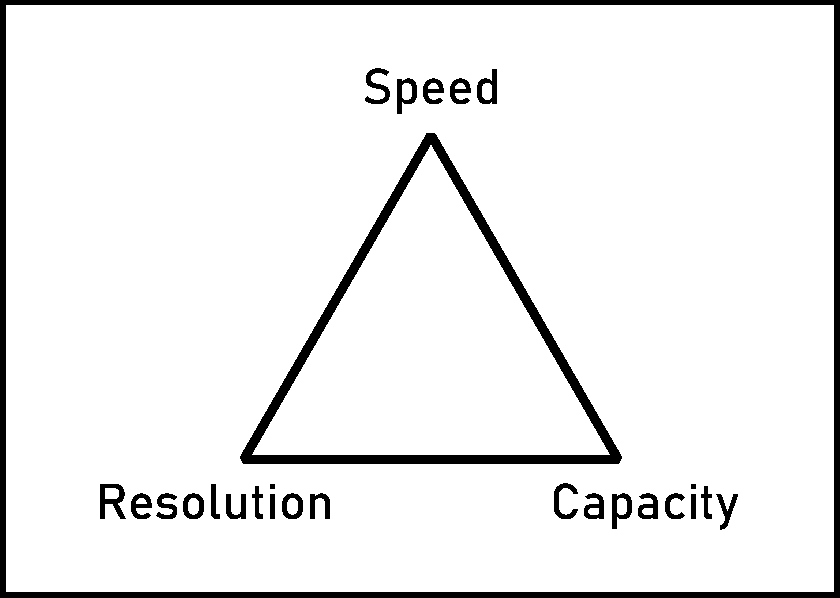
\includegraphics[width=0.75\textwidth]{Figures/Triangle.pdf}
\decoRule
\caption[Schematic diagram of a the chromatographer's trilemma.]{The chromatographer's trilemma.}
\label{fig:trilemma}
\end{figure}


Every chromatographer involved in a kinetic optimization has met the
chromatographer's trilemma (See Figure \ref{fig:trilemma}): Any chromatographic
method that involves decisions about speed, resolution, and capacity can
maximize only one at a time\footnote{This trilemma applies only to capillary
chromatography. When using packed columns, the capacity can be readily increased
by using a column with a larger diameter and a larger amount of packing.}. The
fastest chromatography will have low capacity and low resolution, the
chromatography giving the highest resolution will be slow with low capacity, and
the chromatograpy of a sample with a high concentration of analyte will be slow
and have low resolution \autocite{Klee2002}. One way the chromatographer can
ease the grip of the trilemma is to decide what factor is least important for
the current problem, pick a value for that is likely to be satisfactory for most
conditions, keep it fixed, and then find an acceptable compromise between the
other two. In the development of the SFC×GC we decided to work with a fixed
sample capacity: we chose a capillary column with a \SI{0.25}{\milli\metre}
internal diameter and a \SI{0.25}{\micro\metre} stationary phase. With the
sample capacity held constant, it is now possible to optimize the system so that
it gives adequate resolution in the shortest possible time.

The \keyword{efficiency} of a column is given by the relationship \(E =
\frac{t_R}{\sigma} \), where \(t_R\) is the \keyword{retention time} of a peak,
and \(\sigma\) is its standard deviation, related to the \keyword{peak width}
\autocite{Blumberg2018}. The efficiency is a measure of how much the peak spread
during its transport through the column relative to distance it travelled, using
time as a proxy for distance. Efficiency is related to the more traditional but
less intuitive \keyword{number of plates} \(N\) through the expression \(N =
E^2\). The length of the column (\(L\)), divided by the square of the efficiency
gives the \keyword{plate height} (\(H\)). Plate height is a measure of how much
each unit of length of the column contributes to the separation: a lower \(H\)
means that the separation is more effective. The value of \(H\) in chromatographic
theory is that equations can be developed that express \(H\) as functions of the
adjustable parameters of kinetic optimization. Such functions help predict
suitable chromatographic conditions and set limits to the expected performance
of the separation.

When doing chromatography, any optimization goal must contain resolution as part
of the criteria; after all, the purpose of the activity is the separation of
chemical compounds. Traditionally, the first optimization taught is the
optimization of \(H\) as criterion, with the rate at which the carrier gas
passes through the column as the variable parameter. The rate can be
characterized by either the average gas velocity (\(\overline{u}\)) or the gas
flow rate (\(F\)). Traditionally \(\overline{u}\) have been used, because it can
be conveniently calculated from simple measurements: \(\overline{u} = L/t_m\),
where \(t_m\) is the \keyword{void time}, which is easily determined by
measuring the retention time of an unretained compound. In modern gas
chromatographs \(F\) can be continuously controlled by electronic pneumatic
control (EPC) systems, and has become a more convenient parameter.

Blumberg has developed the theory of optimized flow rate
\autocite{Blumberg1999}. He found that the function that describes plate height
in terms of flow rate can be simplified to two cases: a high-pressure drop and a
low-pressure drop. (A high pressure drop is defined as the case when the
difference in pressure between the inlet and outlet is much greater than the
outlet pressure, \(\Delta{p} \gg p_o\)). When the pressure drop is low 

\(H = \frac{\displaystyle b}{\displaystyle F}+(c_1+c_2)F \)

and when the pressure drop is high

\(H = \frac{\displaystyle 9}{\displaystyle 8} \left(\frac{b}{F}+c_{1}F \right)+C_{2}\sqrt{F}\)

where \(c_1\), \(c_1\) and \(C_2\) are constants independent of \(F\).

When the layer of stationary phase is thin, also known as the \keyword{thin-film
case}, then \(c_2 = 0\) and \(C_2 = 0\), and

\(H = \frac{\displaystyle b}{\displaystyle F} + c_{1} F \) 

for the low pressure drop case and 

\(H = \frac{\displaystyle 9}{\displaystyle 8} \left(\frac{b}{F}+c_{1}F \right)\)

for the high pressure drop case. The low pressure drop case will be immediately
recognized as the \keyword{van Deemter equation}, and the high-pressure drop
case differs from it only by a factor of \num{0.125}. (See Figure
\ref{fig:VanDeemter})

\begin{figure}
\centering
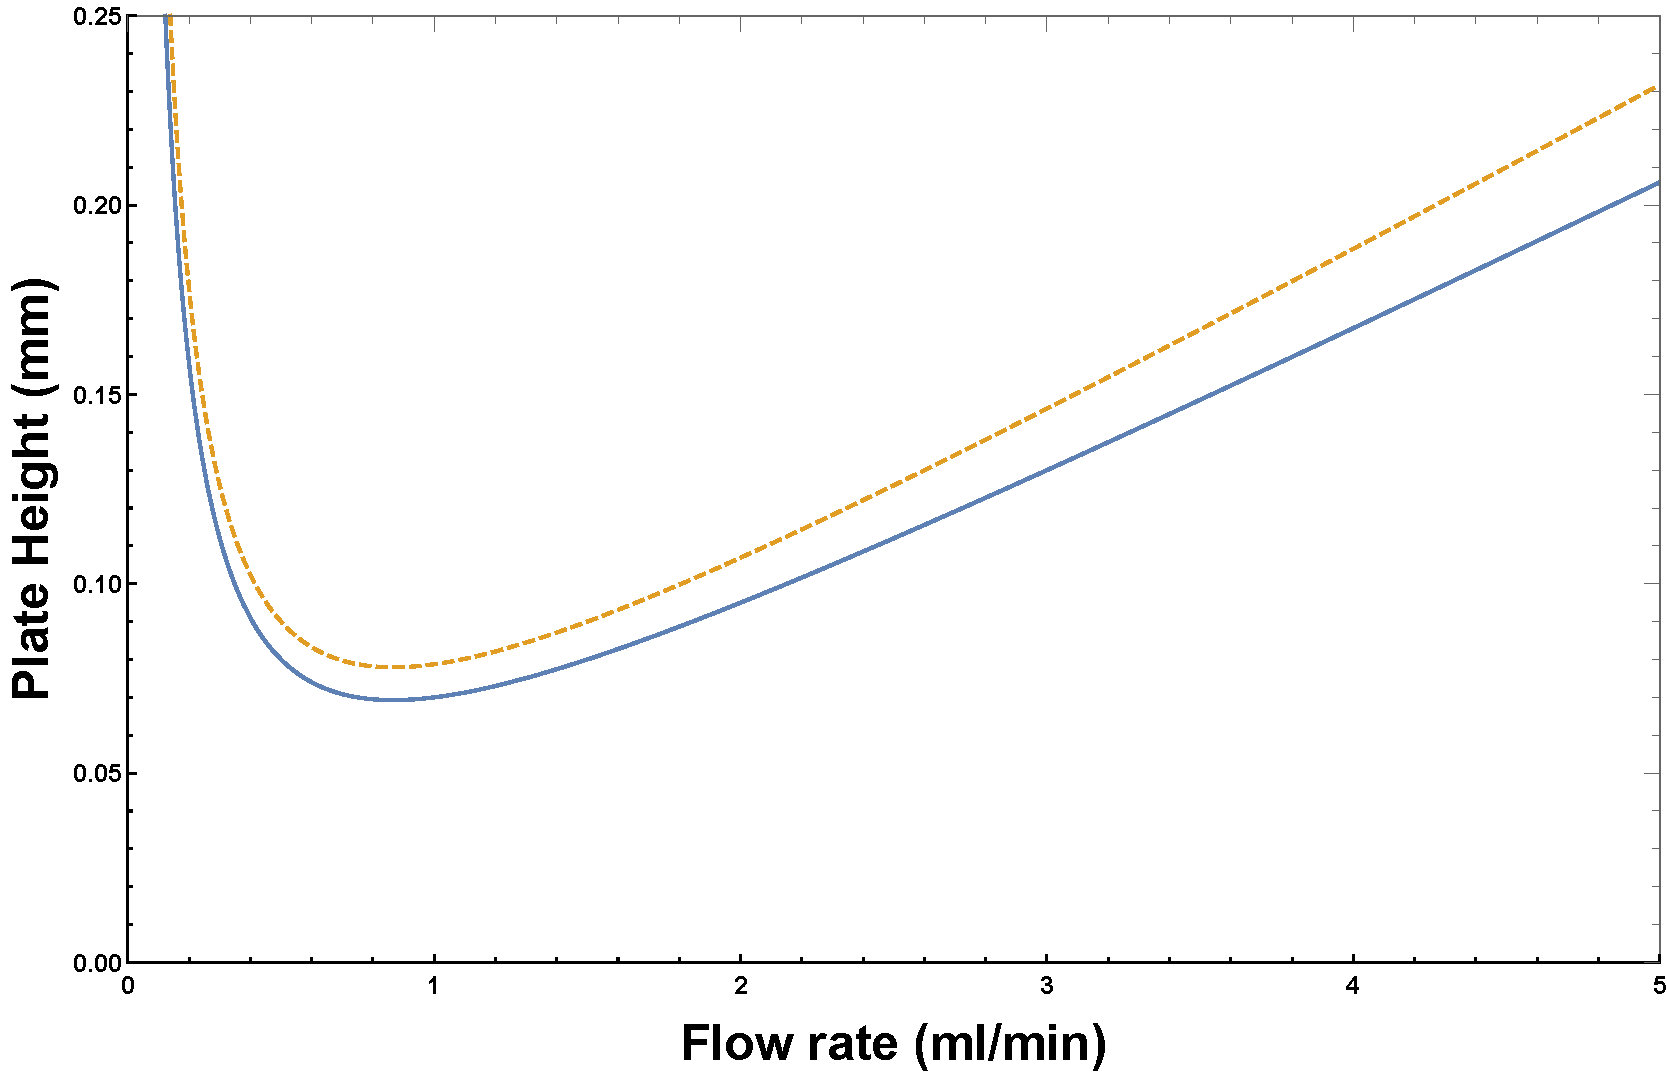
\includegraphics[width=0.75\textwidth]{Figures/VanDeemter.pdf}
\decoRule
\caption[A plot of H \textit{vs.} F]{A plot of H \textit{vs.} F.}
\label{fig:VanDeemter}
\end{figure}

It is clear that the function has a minimum, and the flow rate at this minimum
\(H\) can be called \(F_{Hmin}\). This flow is called
\keyword{efficiency-optimized flow}, EOF. A remarkable feature of this
theoretical result is that it is independent of column length
\autocite{Blumberg1999}. In contrast, the \keyword{efficiency optimized
velocity} (EOV) depends on the column length when the pressure drop is high
\autocite{Blumberg1997}. Because \(E = \sqrt{\frac{L}{H}} \) it means that any
necessary resolution can be obtained by making the column as long as necessary.
This theoretical result is supported by experiment: the world record for the
longest capillary column is \SI{1300}{\metre}. ``This column produced excellent
resolution of a petroleum sample, but took 3 hours to elute methane and 3 days
to elute the last peak'' \autocite{Ferguson2013}. Reducing the column length
while keeping EOF will reduce the column efficiency, although the plate height
will remain constant.

In this study the aim is to reduce the time it takes to complete a run, and
therefore the question is not what the best possible efficiency is, but what the
shortest time is in which a specified efficiency can be maintained. The
remarkably simple theoretical result is that under \keyword{speed-optimized
flow} (SOF), \(F = \sqrt{2}F_{Hmin}\) \autocite{Blumberg1997}. Because this flow
is higher than the EOF, \(H\) is larger, but this can be compensated for by
increasing \(N\), which is implemented by using a longer column. For a given
solute, column diameter, stationary phase and carrier gas there is no flow that
will yield a faster separation without reducing the efficiency of the separation.

The remaining parameters that can be manipulated to kinetically optimize for
speed are column diameter and carrier gas diffusion. The theoretical details
will not be discussed here, but it will be clear that optimizing for separation
speed tends towards the selection of narrow-bore capillary columns and using
hydrogen as a carrier gas. The theoretical study of optimization gives great
insight into which parameters to choose, but the actual calculation can be
tedious, so for practical purposes the use of online method translation
calculators is recommended \autocite{Restek2014}. The improvement possible in
separation speed by using method translation calculations is remarkable, but
still falls short of the speed that is needed for comprehensively coupled
chromatography.

SOF improves the speed of analysis by finding the combination of parameters
\(F\) and \(L\) that will give the fastest separation under the constraint of
constant \(H\). If the constraint on \(H\) is relaxed, a faster separation can
be achieved. Assuming that it is not possible to optimize the selectivity
further (for example because the stationary phase cannot be changed), there are
only two ways to relax the plate height constraint: \keyword{selective
detection} and \keyword{sample cleanup}. In selective detection a detector is
chosen that only responds to the analytes, and not to any interfering compounds.
For example, an \keyword{electron capture detector} (ECD) responds strongly to
halides, so a GC-ECD chromatogram of a soil extract will be much simpler than
the equivalent GC-FID chromatogram, which means that the GC-ECD analysis of
chlorinated pesticides in soil can be much faster than the equivalent GC-FID
analysis. GC-MS using \keyword{single ion monitoring} (SIM) also enables faster
chromatography by simplifying the chromatogram. In sample cleanup the efficiency
constraint can be relaxed because the sample becomes chemically simpler. For
example, a sample might be passed through a \keyword{solid phase extraction}
(SPE) cartridge before it is injected into the chromatograph. Interfering
compounds are retained in the cartridge, which simplifies the sample. A simpler
sample requires lower efficiency, so the SOF can be higher.

The high speed chromatography that is used in GC×GC is possible because any
fraction collected from the \oneD separation is considerably simpler than the
original sample, and therefore the efficiency constraint is relaxed, which
allows a much higher SOF and therefore a very fast \twoD separation. Even at
SOF, there might still be excess efficiency, which could be traded for higher
speed. Since \(E^2 = \frac{H}{L} \), this higher speed can be obtained by
increasing the flow beyond SOF (decreasing \(H\)), or by using a shorter column
(decreasing \(L\)). Optimization with the goal of the best speed/efficiency
ratio using column length and flow as optimizing parameters, theory and
experiment shows that flow nearer the SOF combined with shorter columns give
better performance \autocite{Klee2002, Reed1999} than flow much faster than SOF
combined with longer columns.

\section{The General Elution Problem.}

The theory developed above is for kinetic optimization: it assumes a single
\keyword{retention factor}, \(k'\). This means that the optimization is focused
on the kinetic conditions required to optimally separate two compounds eluting
after each other, which have similar retention behaviour. If a sample were to
contain only these two compounds, then all would be well. But if another pair of
compounds, with a mutually similar retention behaviour but retention behaviour
very different from the first pair were to be separated, the optimum conditions
will be very different. So not all the compounds in complex mixture can be
optimally separated with a single set of conditions. This is known as the
\keyword{general elution problem} \autocite[p. 779]{Skoog2007}. The general
elution problem makes speed and resolution mutually exclusive: a fast
chromatogram will not meet satisfy resolution constraints, and a fully resolved
chromatogram will not satisfy speed constraints.

The solution to the general elution problem is to adjust the conditions during
the run so that the retention factors \(k'\) stay constant during the run. This
strategy is implemented in LC by \keyword{gradient elution}, and in GC by
\keyword{temperature programming}. In isothermal GC less volatile compounds
exhibit higher \(k'\) than more volatile compounds. If kinetic conditions are
optimized for the more volatile compounds, then they will elute optimally, but
the heavier compounds will elute with with excess resolution. If --- after the
elution of the more volatile compounds --- the temperature of the column is
increased, then \(k'\) of the less volatile compounds will increase, so that the
selectivity conditions will now match the optimized kinetic conditions, and
their elution will be optimal. By careful programming the temperature can be
continuously controlled so that the selectivity conditions always match the
kinetic conditions, and all the compounds elute under optimum conditions. The
technology for \keyword{temperature programming} in GC is mature, and every
column manufacturer specifies temperature limits for isothermal and ramped
temperature programs for every stationary phase.

In GC×GC the general elution problem appears in the form of
\keyword{wrap-around}, defined as ``the occurence of second dimension peaks in
subsequent modulation sequences, caused by second-dimension retention times that
exceed the modulation period of a comprehensive two-dimensional system''
\autocite{Mariott2012}. In GC×GC the \twoD separation is isothermal, but because
GC separations are predominantly determined by volatility, in the \twoD
separation the retention factors have similar values and wrap-around is just a
nuisance. In SFC×GC, where the group-type separation on the \oneD column yields
fractions that contain compounds with a wide range of volatilities
\autocite{Venter1999a}, isothermal GC will have unacceptable wrap-around.
Therefore, temperature programming is necessary for successful SFC×GC.

Guided by the theory described above, the fast GC used as the \twoD  separation
in the SFC×GC chromatograph was designed to use a short GC column
(\SI{1}{\metre} long) with flow higher than SOF that follows a correspondingly
fast temperature program.

\section{Temperature ramp rates}
\label{sec:RampRates}

Early experimenters realized the importance of temperature control in GC, and
used vapour baths \autocite{Desty1957} or oil baths \autocite{Eggertsen1956} to
control temperature in their experiments, but they quickly realized that leaks
or cracks could allow oil into the column. Oil that entered the column would
then contaminate the stationary phase, rendering it useless.  If air is used to
transfer heat to the column, the gas pressure inside the column is higher than
the atmospheric air pressure outside the column, so leaks let carrier gas escape
but does not allow contaminants to enter. Therefore, in the modern gas
chromatograph the convention is to control the temperature of GC columns by
keeping them immersed in an air bath with a precisely controlled temperature. 

A temperature program is traditionally described using a series of
\keyword{ramps} and \keyword{holds.} A ramp is a period of time during which the
temperature changes, almost always increasing. The \keyword{ramp rate} is the
rate at which the temperature changes. A hold is a period of time during which
the temperature is kept constant.

When developing a chromatographic method, at what rate must the temperature of a
column increase so that the selectivity conditions match the kinetic conditions?
Blumberg and Klee \autocite{Blumberg2000} recommend that a good initial
temperature ramp rate is \SI{10}{]\celsius} per void time ($t_m$). For long
columns the void times are long, and the ramp rates can be low. As an
illustration, Figure \ref{fig:RampRate7890B} shows the temperature ramp rates of
a state-of-the-art chromatograph. By contrast, for short, narrow-bore columns,
the ramp rate needs to be thousands of \SI{}{\celsius\per\minute}.

\begin{figure}
	\centering
	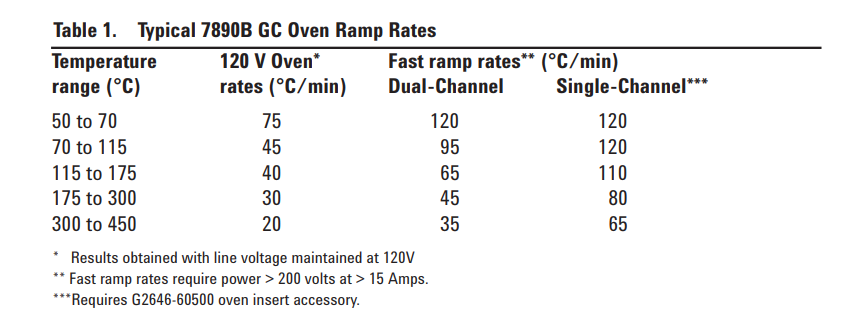
\includegraphics[width=0.8\textwidth]{Figures/7890B.png}
	\decoRule
	\caption[A temperature-rate table from the Agilent7890B data sheet]{The
	temperature-rate table from the Agilent 7890B chromatograph data sheet
	\autocite{7890B}. }
	\label{fig:RampRate7890B}
\end{figure}

The low ramp rate of conventional air baths is caused by three factors:

\begin{itemize}
	\item The low heat capacity of air
	\item The poor thermal conductivity of air
	\item The mass of the oven that needs to be heated. 
\end{itemize}

There is very little that can be done about these matters. It would be possible
to switch oven gas to hydrogen for higher thermal conductivity, and construct a
low-mass oven using, say, advanced resins for construction, but this would
probably involve significant safety and cost issues. What is required is a
complete redesign of the heating principle.

\subsection{Resistive heating}

Fortunately, the heating rate problem has a technologically simple solution,
\keyword{resistive heating}\footnote{Alternative methods of heating by
electromagnetic fields are \keyword{inductive heating} and \keyword{dielectric
heating}.}. When a constant electric field is applied to a metal, the free electrons in
the metal will be accelerated by the electric field. But the electrons are
within the crystal lattice of the metal, where their mean free path is very
short. The electrons will therefore collide with atoms in the crystal lattice,
scattering inelastically. The energy lost in the inelastic collisions will
increase the vibrational frequency of atoms, and this energy will appear as
heat.

The number of electrons and their average (drift) speed in combination is
described by a measure called the \keyword{current} ($I$), and the electric field
is can be described by the applied \keyword{voltage} ($V$). The current $I$ is
proportional to the applied voltage, and the ratio $\frac{V}{I}$ defines a
proportionality constant $R$, called the resistance, which is a function of
the conductor's material and dimensions. The total power dissipated to heat ($P$) is
given by $P=IV$ or, equivalently, $P=I^2R$ or $P=\frac{R}{V^2}$.

Applying a voltage \(V\) to a metal element close to a chromatographic column
will heat the metal, and therefore the column in contact with it. The rate at
which the piece of metal heats up depends on the power dissipated, the mass of
the metal, and its heat capacity. If the volume of the metal is small enough,
and the current high enough, the temperature of the metal element (and with it
the temperature of the column) will increase at a rate high enough to be useful
in chromatography. By suitable manipulation of \(V\), then, the temperature of
the column can then be changed at any desirable rate.

This technology has been reviewed \autocite{Wang2012, Jacobs2013, Miranda2010},
and a few technologies for resistive heating of capillary columns have emerged:

\begin{itemize}
  \item Direct heating of a metal column or a column coated with a metal layer
  \item Collinear heating
  \item Coaxial heating
\end{itemize}

The first SFC×GC work done \autocite{Venter2004} used a directly heated metal
column. While this approach proved the concept, experience showed two
shortcomings. Firstly, metallic columns are usually designed with specific
high-temperature applications in mind. This means that metal columns are not
available with all the stationary phases available in fused-silica columns.
Secondly, it was harder than expected to control the temperature accurately. The
temperature was determined by a thermocouple glued to the column, which was
sensitive to local variations.

An example of collinear resistive heating is Agilent\texttrademark{}'s
`low thermal mass' column, which includes collinear heating wire and a collinear
sensing element bundled with a short fused silica column. This approach requires that
the collinear heating element be wrapped in close contact with the column.

For the work presented in this thesis, a coaxial heater was used. This heater is
in the form of a thin-walled stainless-steel tube that carries the electric
current. It was made of a \SI{940}{\milli\metre} length of SAE 304 stainless
steel with an outside diameter of \SI{1.06}{\milli\metre} and an inside diameter
of \SI{0.80}{\milli\metre}. The column was threaded inside the stainless steel
tube, which put it in close contact with the heater, giving reliable heat
transfer.
The coaxial heater can be coiled to fit inside a conventional GC oven.

This coaxial design has the advantage that the column can be changed without
changing the resistive heater. This means that there is no need to re-calibrate
the heater when columns are changed.

\begin{figure}[htbp]
	\centering
	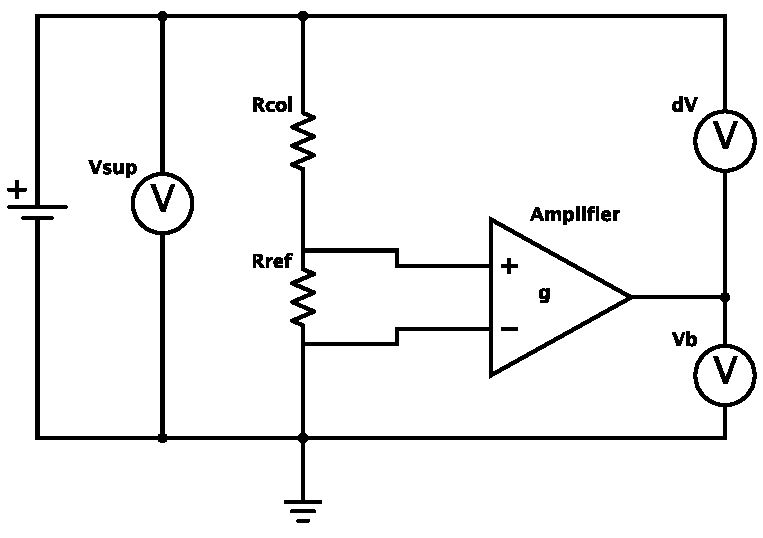
\includegraphics[width=0.8\textwidth]{Figures/Column-Heater.pdf}
	\decoRule
	\caption[Coaxial heater resistance heater]{\label{fig:HeaterDiagram}Electric circuit diagram of the coaxial heater.}
\end{figure}

The electrical resistance of a conductor is determined by its dimensions, the
material it is made of, and the temperature of that material. In a conductor of
given dimensions, therefore, a knowledge of the resistance implies a knowledge
of the temperature. By following changes in the resistance, one can determine
changes in the temperature, and by comparing resistance at certain temperatures
with known temperatures, one can get a calibrated temperature from a given
resistance.

High-powered resistive heating implies low resistance. Measuring the
\emph{absolute value} of low resistance is technologically challenging
\autocite{Dyos2012}. But a simple electronic circuit can be used to
\emph{compare} the resistance of the coaxial heater with that of a reference
resistor (Figure \ref{fig:HeaterDiagram}). The circuit is supplied by a voltage
\(V_{sup}\), in general an unknown value.
\(V_{col}\) and \(V_{ref}\) represents the voltage drop over the respective
resistors. Because the current \(I\) through the circuit is the same for both
\(R_{col}\) and \(R_{ref}\), it is true that
\(\frac{R_{col}}{V_{col}} = \frac{ R_{ref} }{ V_{ref} }\), and therefore

\(R_{col} = R_{ref}\frac{V_{col}}{V_{ref}}\)

The voltage drop across $R_{ref}$ is too small to be directly digitized,
therefore it is amplified by an amplifier with gain $g$, so that $V_b =
gV_{ref}$. $V_b$ is measured, as is $dV$, the potential difference between the
supply and the amplifier output. We can show that the coaxial heater resistance
\(R_{col}\) is a function of the voltage ratio \(\frac{dV}{V_b}\).

First, 
\[ V_{sup} = V_{col} + V_{ref} \] 
but also
\[ V_{sup} = dV + V_b \]
Therefore,
\[ V_{col} + V_{ref} = dV + V_b \]
But \(V_{b} = g V_{ref}\), so
\[ V_{col} + V_{ref} = dV + gV_{ref} \]

\[ V_{col} = dV + gV_{ref} - V_{ref} \]

\[ V_{col} = dV + V_{ref}(g - 1) \]

\[ \frac{\displaystyle V_{col}}{\displaystyle gV_{ref}} = dV/gV_{ref} + V_{ref}(g-1)/gV_{ref} \]

\[\frac{\displaystyle V_{col}}{\displaystyle V_{ref}} = gdV/gV_{ref} + gV_{ref}(g-1)/gV_{ref} \]

\[\frac{\displaystyle V_{col}}{\displaystyle V_{ref}} = g\frac{dV}{V_b} + (g-1) \]

This proves that \( \frac{\displaystyle V_{col}}{\displaystyle V_{ref}} \) is a
linear function of $dV/V_b$. A quick check for correctness of the expression:
for a unity-gain amplifier $g = 1$, and $\frac{\displaystyle
V_{col}}{\displaystyle V_{ref}} = dV/V_b$.

Therefore 

\[ R_{col} = R_{ref} \left(\frac{g{dV}}{V_b} + (g-1) \right) \]

In practice the gain \(g\) might not be completely constant, but show a slight
dependence on \(dV\), so a general expression might be

\[ R_{col} = f\left(\frac{dV}{V_b} \right) \]


\section{Calibration}

The assumption is that the temperature is a function of the resistance of the
coaxial heater, or \( T = g(R_{col}) \). Because \( R_{col}=f(\frac{dV}{V_b}) \),
we can see that \( T = g(f(\frac{dV}{V_b})) \), or, because a function \(g\) of
a function \(f\) is a function \(h\) (\(f \circ g = h \)), \( T =
h(\frac{dV}{V_b}) \).  Through a calibration procedure \(h\) can be
approximated by a polynomial or lookup table.

\subsection{Temperature uniformity}
\label{sec:Uniformity}

It is highly desirable that the coaxial heater should give uniform heating, but
there is no obvious guarantee an electrically heated tube will heat uniformly.
We did not analyse the problem theoretically, but the following factors will
play a role:

\subsubsection{Resistivity's dependence on temperature}

The resistance of a metal increases with temperature. This means that if one
section of the coaxial heater gets hotter than the rest, its resistance
will increase. If the current were to remain constant, more power would be
dissipated in this section (\(P=I^2R\)). If more power is dissipated, the
temperature will increase, leading to a higher resistivity, leading to higher
power dissipation, leading to a higher temperature, in a runaway cycle. In
contrast, if the coaxial heater was made of a material of which the resistivity
decreases with an increase in temperature, the temperature along the length of
the heater would be stabilized by negative feedback. In the case of the supply
voltage being held constant a higher resistance in one section would mean a
lower current overall, but still a higher power dissipation in the section with
higher temperature.

\subsubsection{Thermal conduction}

Each section of the coaxial heater is in thermal contact with its neighbours. If
it were to get hotter, the heat will flow from the hotter section to the cooler
neighbouring sections. This will tend to even out any temperature differences.

\subsubsection{Radiation}

An object radiates heat, which can be approximated by the Stefan-Boltzman law:

\begin{equation}\label{eq:1}
	P=A \epsilon \sigma T^4
\end{equation}

where A is the surface area of the object, \(\epsilon\) is the
\keyword{emissivity} of the surface, \(\sigma\) is the Stefan-Boltzman constant,
and \(T\) is the absolute temperature of the object. 

If a section of the coaxial heater were to become hotter than the other
sections, it would therefore radiate more heat. The increased power dissipation
by the higher resistance will therefore be partially offset by a higher
radiation. This will tend to moderate temperature differences.

\subsubsection{Convection}

When a part of the coaxial heater is hot, it will heat the air around it,
through radiation and conduction. This air might then move, through buoyancy or
any other force, past another part of the coaxial heater. This second part could
then be heated up by the transported air. For example, a vertically mounted
coaxial heater can be expected to develop a temperature gradient from bottom to
top, as natural convection lets hot air transfer heat from the lower end of the
heater to the upper end. In this way temperature gradients could be established
and maintained.

\subsubsection{Examining thermal uniformity by imaging}

The effect of the combination of resistivity's temperature dependence, thermal
conduction, radiation, and convection on the temperature uniformity of the
coaxial heater could be mathematically or numerically modelled, but such an
endeavour would fall outside the scope of this project. Experience had not led
us to expect any significant temperature non-uniformity, but we welcomed the 
opportunity to get empirical confirmation.

\keyword{Thermal imaging} is the process by which infrared radiation from
objects can be captured in a photographic process. At near-ambient temperatures
objects emit copious amounts of infrared radiation, and higher the temperature,
the more is emitted. (See Equation \ref{eq:1}.) Cameras designed using
specialized optics and sensors allow the capture of that radiation as an image
of a scene that shows objects based on their surface temperature. The
technological capability of thermal imaging has improved markedly over the past
years.

Using a FLIR{\texttrademark} T660 thermal imaging camera we obtained a video of
the coaxial heater executing three consecutive temperature ramps. This camera
uses a \num{640 x 480} focal plane uncooled bolometer array as a detector, which
is sensitive to radiation in the range \SI{7.5}{\micro\metre} to
\SI{14}{\micro\metre}. Figure \ref{fig:ThermalImageSetup} shows the setup used
to record the thermal video. To get reliable temperature information from a
thermal image requires calibration or a precise knowledge about the material's
\keyword{emissivity}. In the absence of such calibration, the obtained
temperature measurement is more useful if seen as relative rather than absolute.

\begin{figure}
	\centering
	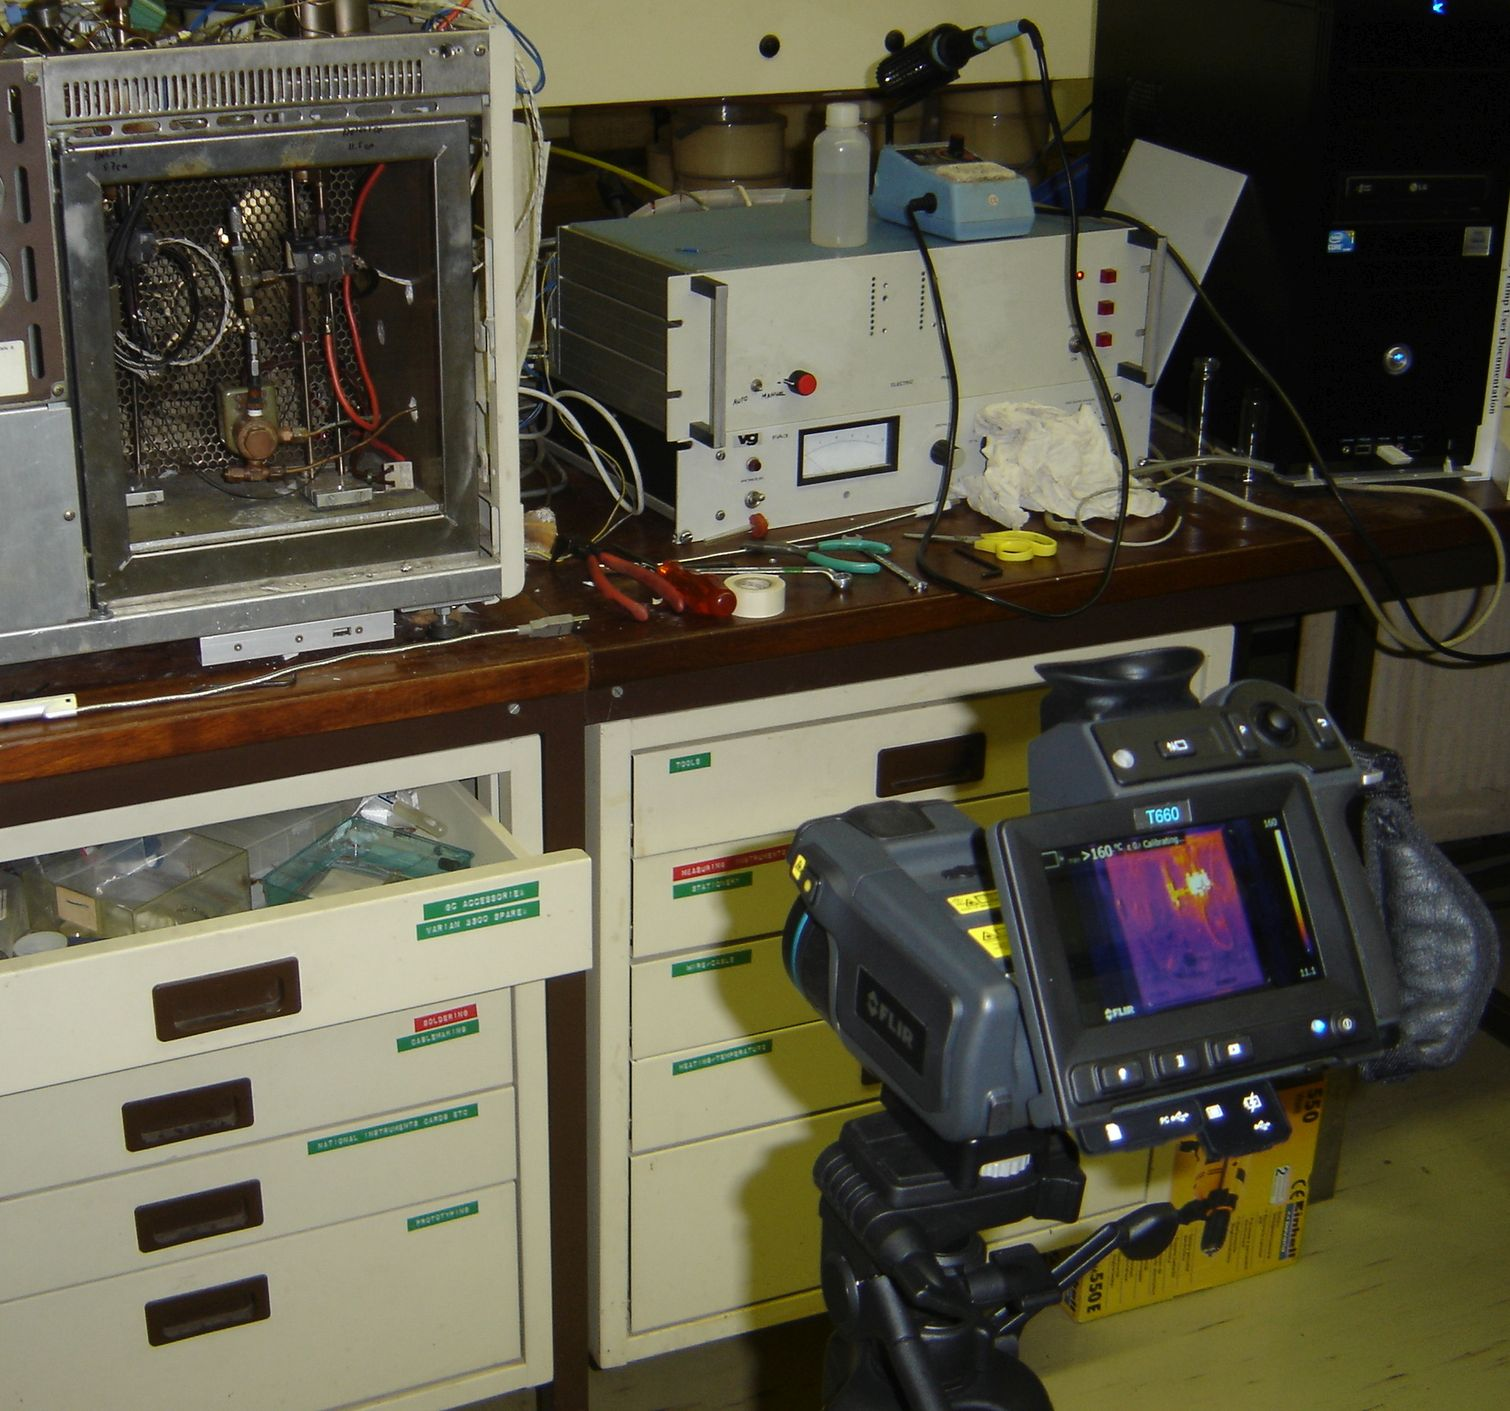
\includegraphics[width=0.8\textwidth]{Figures/ThermalImageSetup}
	\decoRule
	
\caption[A photograph of the setup used to record the thermal video]{This
photograph shows the setup used to record the termal video.}
	
	\label{fig:ThermalImageSetup}
\end{figure}

The video showed that the three consecutive temperature runs heated the coaxial
heater identically. Figure \ref{fig:ThermalImage} is a frame from the video,
analysed to give estimates of the temperatures on spots on the coaxial heater.
The maximum temperature difference between any two points is
\SI{17.5}{\celsius}, and there are no marked gradients.

\begin{figure}
	\centering
	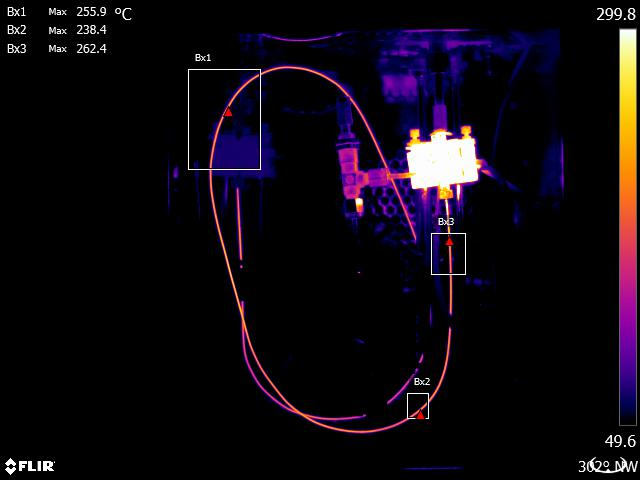
\includegraphics[width=0.8\textwidth]{Figures/ThermalImage}
	\decoRule
	
\caption[A thermograph of the coaxial heater at temperature]{A thermograph of
the coaxial heater at high temperature. It shows that there are no runaway hot
spots.}
	
	\label{fig:ThermalImage}
\end{figure}

This examination of the uniformity of the coaxial heater helped to dispel fears
that unexpected temperature gradients would interfere with the fast gas
chromatography. 

\subsection{Temperature calibration}

When doing temperature-programmed gas chromatography it is desirable to have an
absolute measurement of the column temperatures. This makes it possible to
translate and compare methods between instruments. It was therefore necessary to
calibrate the temperature of the coaxial heater. Calibration is the comparison
of measurement values from a device under test with those of a calibration
standard of known accuracy. In the case of the temperature calibration of the
coaxial heater, it means comparing the results of the temperature as measured by
the coaxial heater with a standard temperature.

The problems of measuring a temperature inside a tube with a bore of
\SI{0.8}{\milli\metre} are not trivial, and to solve them we examined the
available technologies to find the optimum solution.

The following temperature measurement technologies exist:
\begin{itemize}
	\item Liquid-in-glass thermometers
	\item Sealed liquid or gas sensing instruments and bimetallic sensors.
	\item Electrical resistance temperature measurement using metallic sensors
	\item Thermistors and semiconductors
	\item Thermoelectric temperature measurement
	\item Disappearing filament optical pyrometer
	\item Photoelectric optical pyrometers
	\item Total radiation pyrometers.
\end{itemize}

Liquid-in-glass thermometry would not be applicable because of the size of the
devices, and because they don't give a desirable electrical signal. Sealed
liquid or gas sensing elements are also too bulky, and like bimetallic sensors
are best used where only an on/of electric signal is required.

In recent years the technology for measuring temperature by radiant energy
methods have improved markedly and has become affordable, in the form of thermal
cameras. However, at lower temperatures the accuracy of the recorded temperature
depends heavily on the emissivity of the measured material. Thermal imaging will
also only measure the outside wall surface temperature of the heater, and not
the temperature on the inside of the coaxial heater. So, while thermal imaging
settled questions about heater uniformity (Section \ref{sec:Uniformity}), it was
not considered ready to serve as a calibration standard. 

This leaves us with resistance temperature measurement with metallic sensors,
thermistors and semiconductors, and thermoelectric temperature measurement.

Electrical resistance measurement using metallic sensors might have been
feasible, if sensing elements of the appropriate dimensions were commercially
available. A further difficulty with this method of temperature measurement is
that long, thin conductors would be needed to connect the sensing element to the
electronics. These conductors would add to the resistance measured by the
sensing element, requiring complex correction or multi-wire measuring methods.

Thermistor and semiconductor devices could be made small enough, but all
commercially available packages are too large. Besides, the temperature range
used in GC (\SI{-50}{\celsius} to \SI{400}{\celsius}) does not fall inside the
operating temperature range specified by manufacturers of semiconductor devices
(\SI{-55}{\celsius} to \SI{125}{\celsius} for military applications)
\autocite{nullD1996}.

Thermoelectric temperature measurement then remains, and was used to calibrate
the coaxial heater. In particular, the \keyword{Seebeck effect} was exploited,
which is the observation that a temperature gradient imposed on a metallic
conductor will generate an electrical potential along the gradient. Therefore, a
circuit of two dissimilar metallic conductors will generate a voltage when there
is a temperature gradient along the conductors. The voltage generated is a
function of the temperature difference between the hot junction of the two
metals and their cold junctions at the voltmeter input. Such a pair of
dissimilar conductors used to generate a voltage is known as a
\keyword{thermocouple}, and this technology is mature and widely used in
industry. Standard thermocouples are constructed from well-characterized alloys
that generate predictable voltages for given junction temperatures. Pairs of
thermocouple standardized alloys are known as 'types', of which the
general-purpose Type K suited our purpose best. Thermocouple wire can be
purchased in a range of gauges, down to \SI{25}{\micro\metre} in diameter, and the
signal processing for thermocouple signals have been standardized. Thermocouple
junctions can be made by welding, crimping, soft soldering, hard soldering,
bolting, or simply twisting the wires together \autocite{McGee1988}. Because the
temperature range to be measured was ({-}50 \si{\celsius} to 400 \si{\celsius})
soft soldering is not a viable choice, because soft solders have melting points
around \SI{200}{\celsius}. The possibility of corrosion and mechanical vibration
suggest that twisting the wires together will not form a reliable joint, and of
course there are no sub-millimetre bolts on the market.

This leaves welding, crimping and hard soldering as methods for making
thermocouple junctions. Tools for crimping hair-fine wire are rare, and it is
likely that a practical crimped connection will have a diameter many times the
diameter of the wire, possibly making it too large to fit. 

Hard soldering is usually done with a high-temperature flame, and on contact the
flame will rapidly burn the fine wires. The temperature required for hard
soldering is still lower than the melting point of the wires, so that hard
soldering is not excluded, but we did not have the knowledge or the technology
to solve the associated problems.

Welding was found to be an accessible technology for forming small, reliable
joints in fine thermocouple wire.

\subsection{Thermocouple Welding}

Welding is the process of joining two metal parts by melting a portion of each
part, allowing the molten metals first to mix, and then to solidify. This
creates a permanent joint between the two metals. Welding is widely practised as
an industrial process in applications ranging from shipbuilding to
microelectronics. Previous work in our laboratories used capacitive discharge
spot welding to melt the spot where two wires crossed. These thermocouples were
found to be too fragile for the intended application, so a method was developed
to yielded a more robust thermocouple.

In the laboratory electricity is the most convenient sourc of heat. A
\SI{24}{\volt} direct current, adjustable bench power supply was used to supply
the current. The two wires of the thermocouple were twisted together, and the
twisted pair was connected to one pole of the power supply. A carbon electrode
was connected to the other pole. The carbon electrode was carefully brought
closer to the thermocouple pair until a spark jumped across the air gap. When
the spark turned into an arc the heat of the arc melted the end of the twisted
pair. The molten metal would then contract into a spherical globule, which grew
as the arc added more heat. As more of the metal of the wire melted, the globule
would move away from the carbon electrode, until the gap became too large to
sustain the arc. The current would then stop, leaving a spherical welded bead at
the end of the wires. (See Figure \ref{fig:WeldingSteps}.) The process could be
repeated as often as necessary to obtain a bead of the desired size.

It is worth noting that it is necessary to form an arc: if the carbon electrode
happens to touch the wire so that a current flows directly from the wire to the
carbon electrode the wire rapidly heats up over its length and melts. It is also
interesting that it seems necessary to have a roughly broken carbon electrode
surface: a polished surface would not generate an arc, or even make electrical
contact with the wires. This might be because the graphite used for the
electrode was formulated for use in pencils.

The apparatus used to do the welding is depicted in Figure
\ref{fig:FineWireWelder}, and Figure \ref{fig:TCWeldMicro} shows the image seen
through the microscope when the welding is done.

\begin{figure}
	\centering
	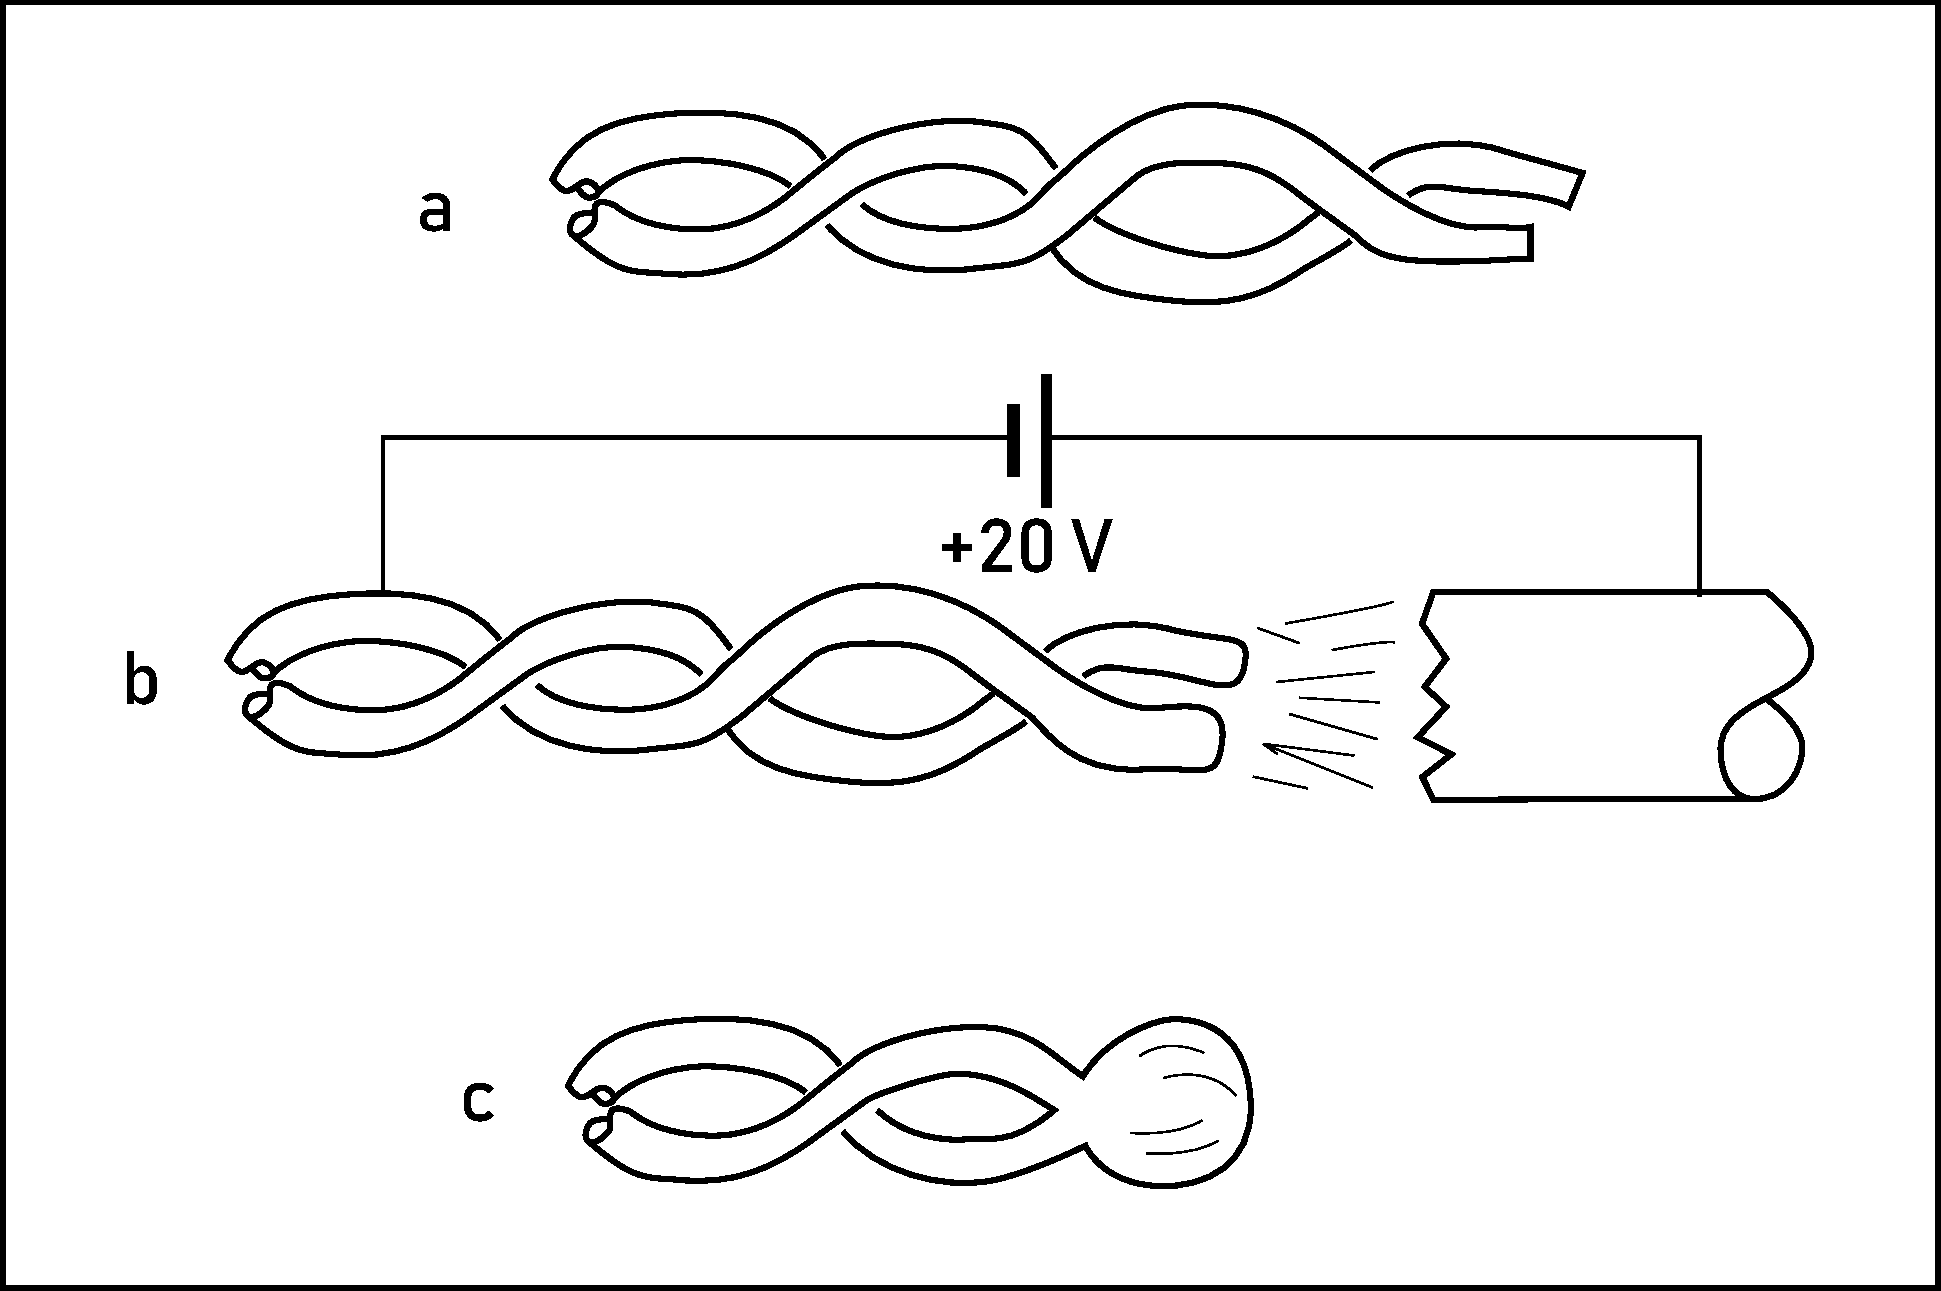
\includegraphics[width=0.8\textwidth]{Figures/TCWelding}
	\decoRule

\caption[Welding process schematic]{The process of welding fine wires to make
thermocouples (a) Wires twisted together (b) Electric arc heating up the wires
(c) Wires welded with a well-formed bead. }

\label{fig:WeldingSteps}
\end{figure}


\begin{figure}
	\centering
	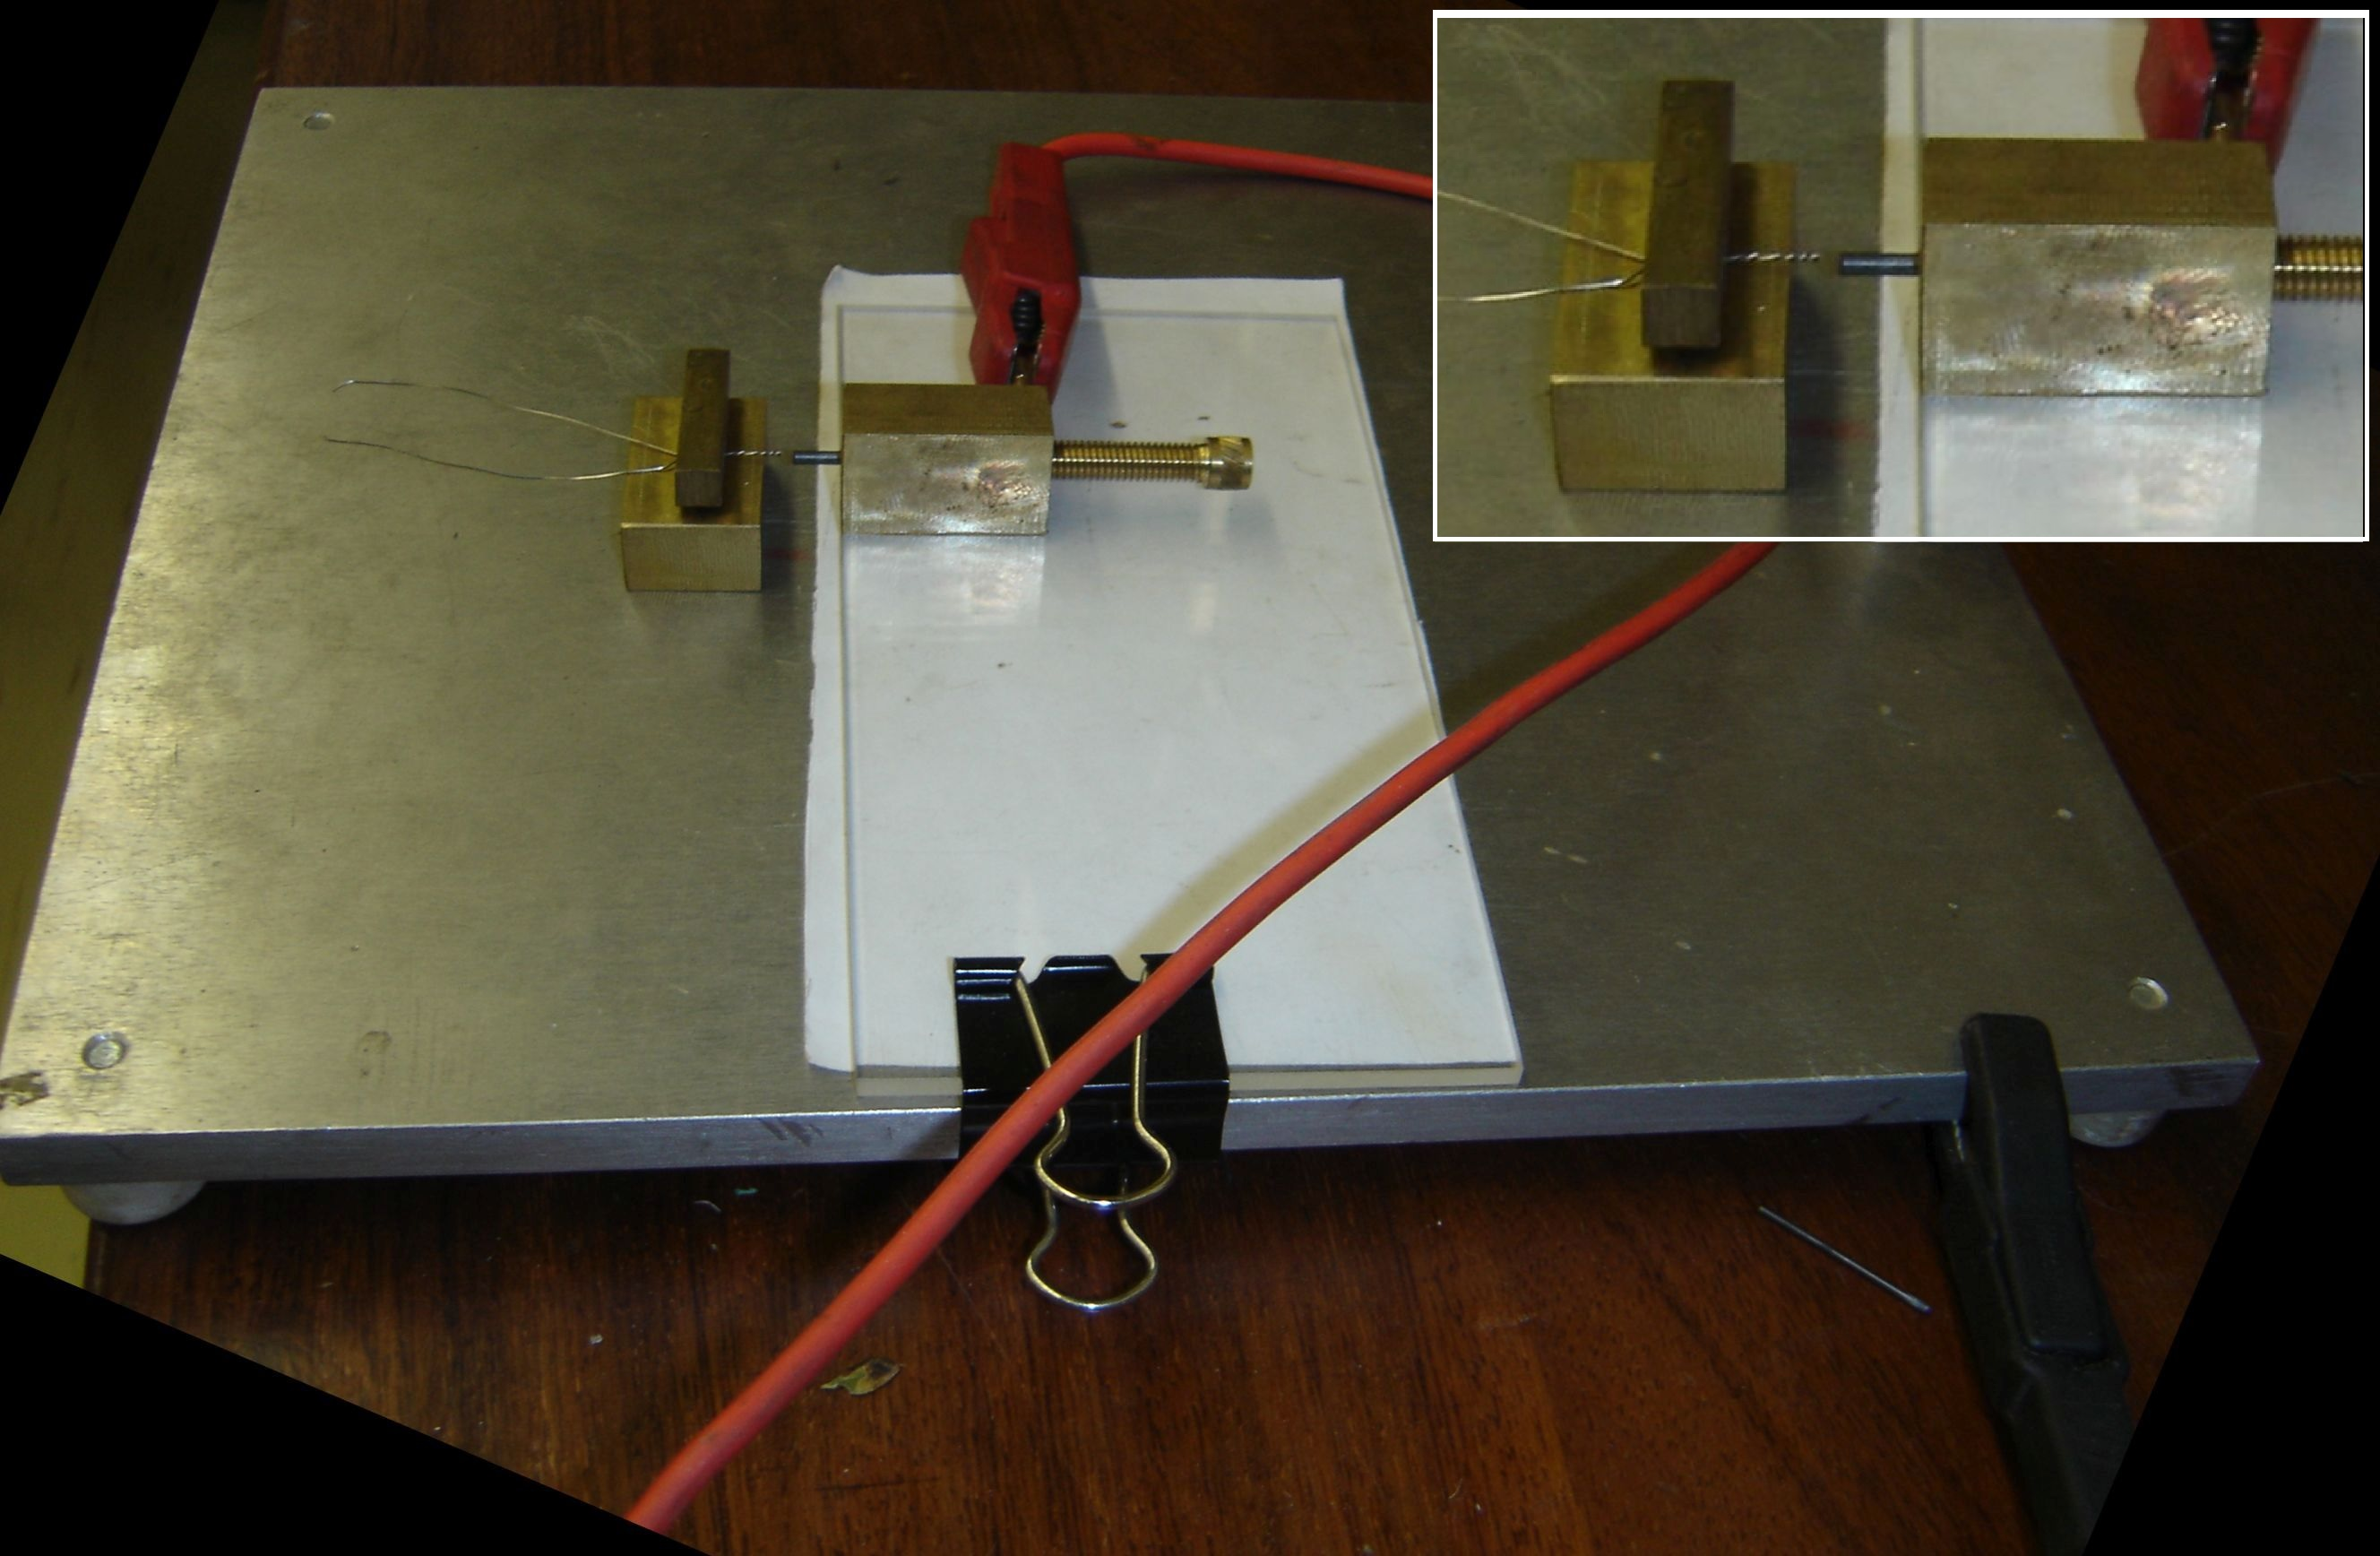
\includegraphics[width=0.8\textwidth]{Figures/Welder3.jpg}
	\decoRule

\caption[Fine-wire welder]{A view of the fine-wire thermocouple welder, as set
up on a microscope base plate. The wire shown in the photograph is much thicker
than that actually used. It is shown clamped between the clamping bar and the
clamping weight. A thin sheet of acrylic serves to isolate the positive
electrode from the negative base. The carbon electrode can be advanced towards
the thermocouple twist using the screw. The black clamp at the bottom right-hand
corner attached to the base plate and the red clamp attached to the screw
housing provide a potential difference of approximately \SI{20}{V} between the
carbon electrode and the thermocouple. }

\label{fig:FineWireWelder}
\end{figure}

\begin{figure}
	\centering
	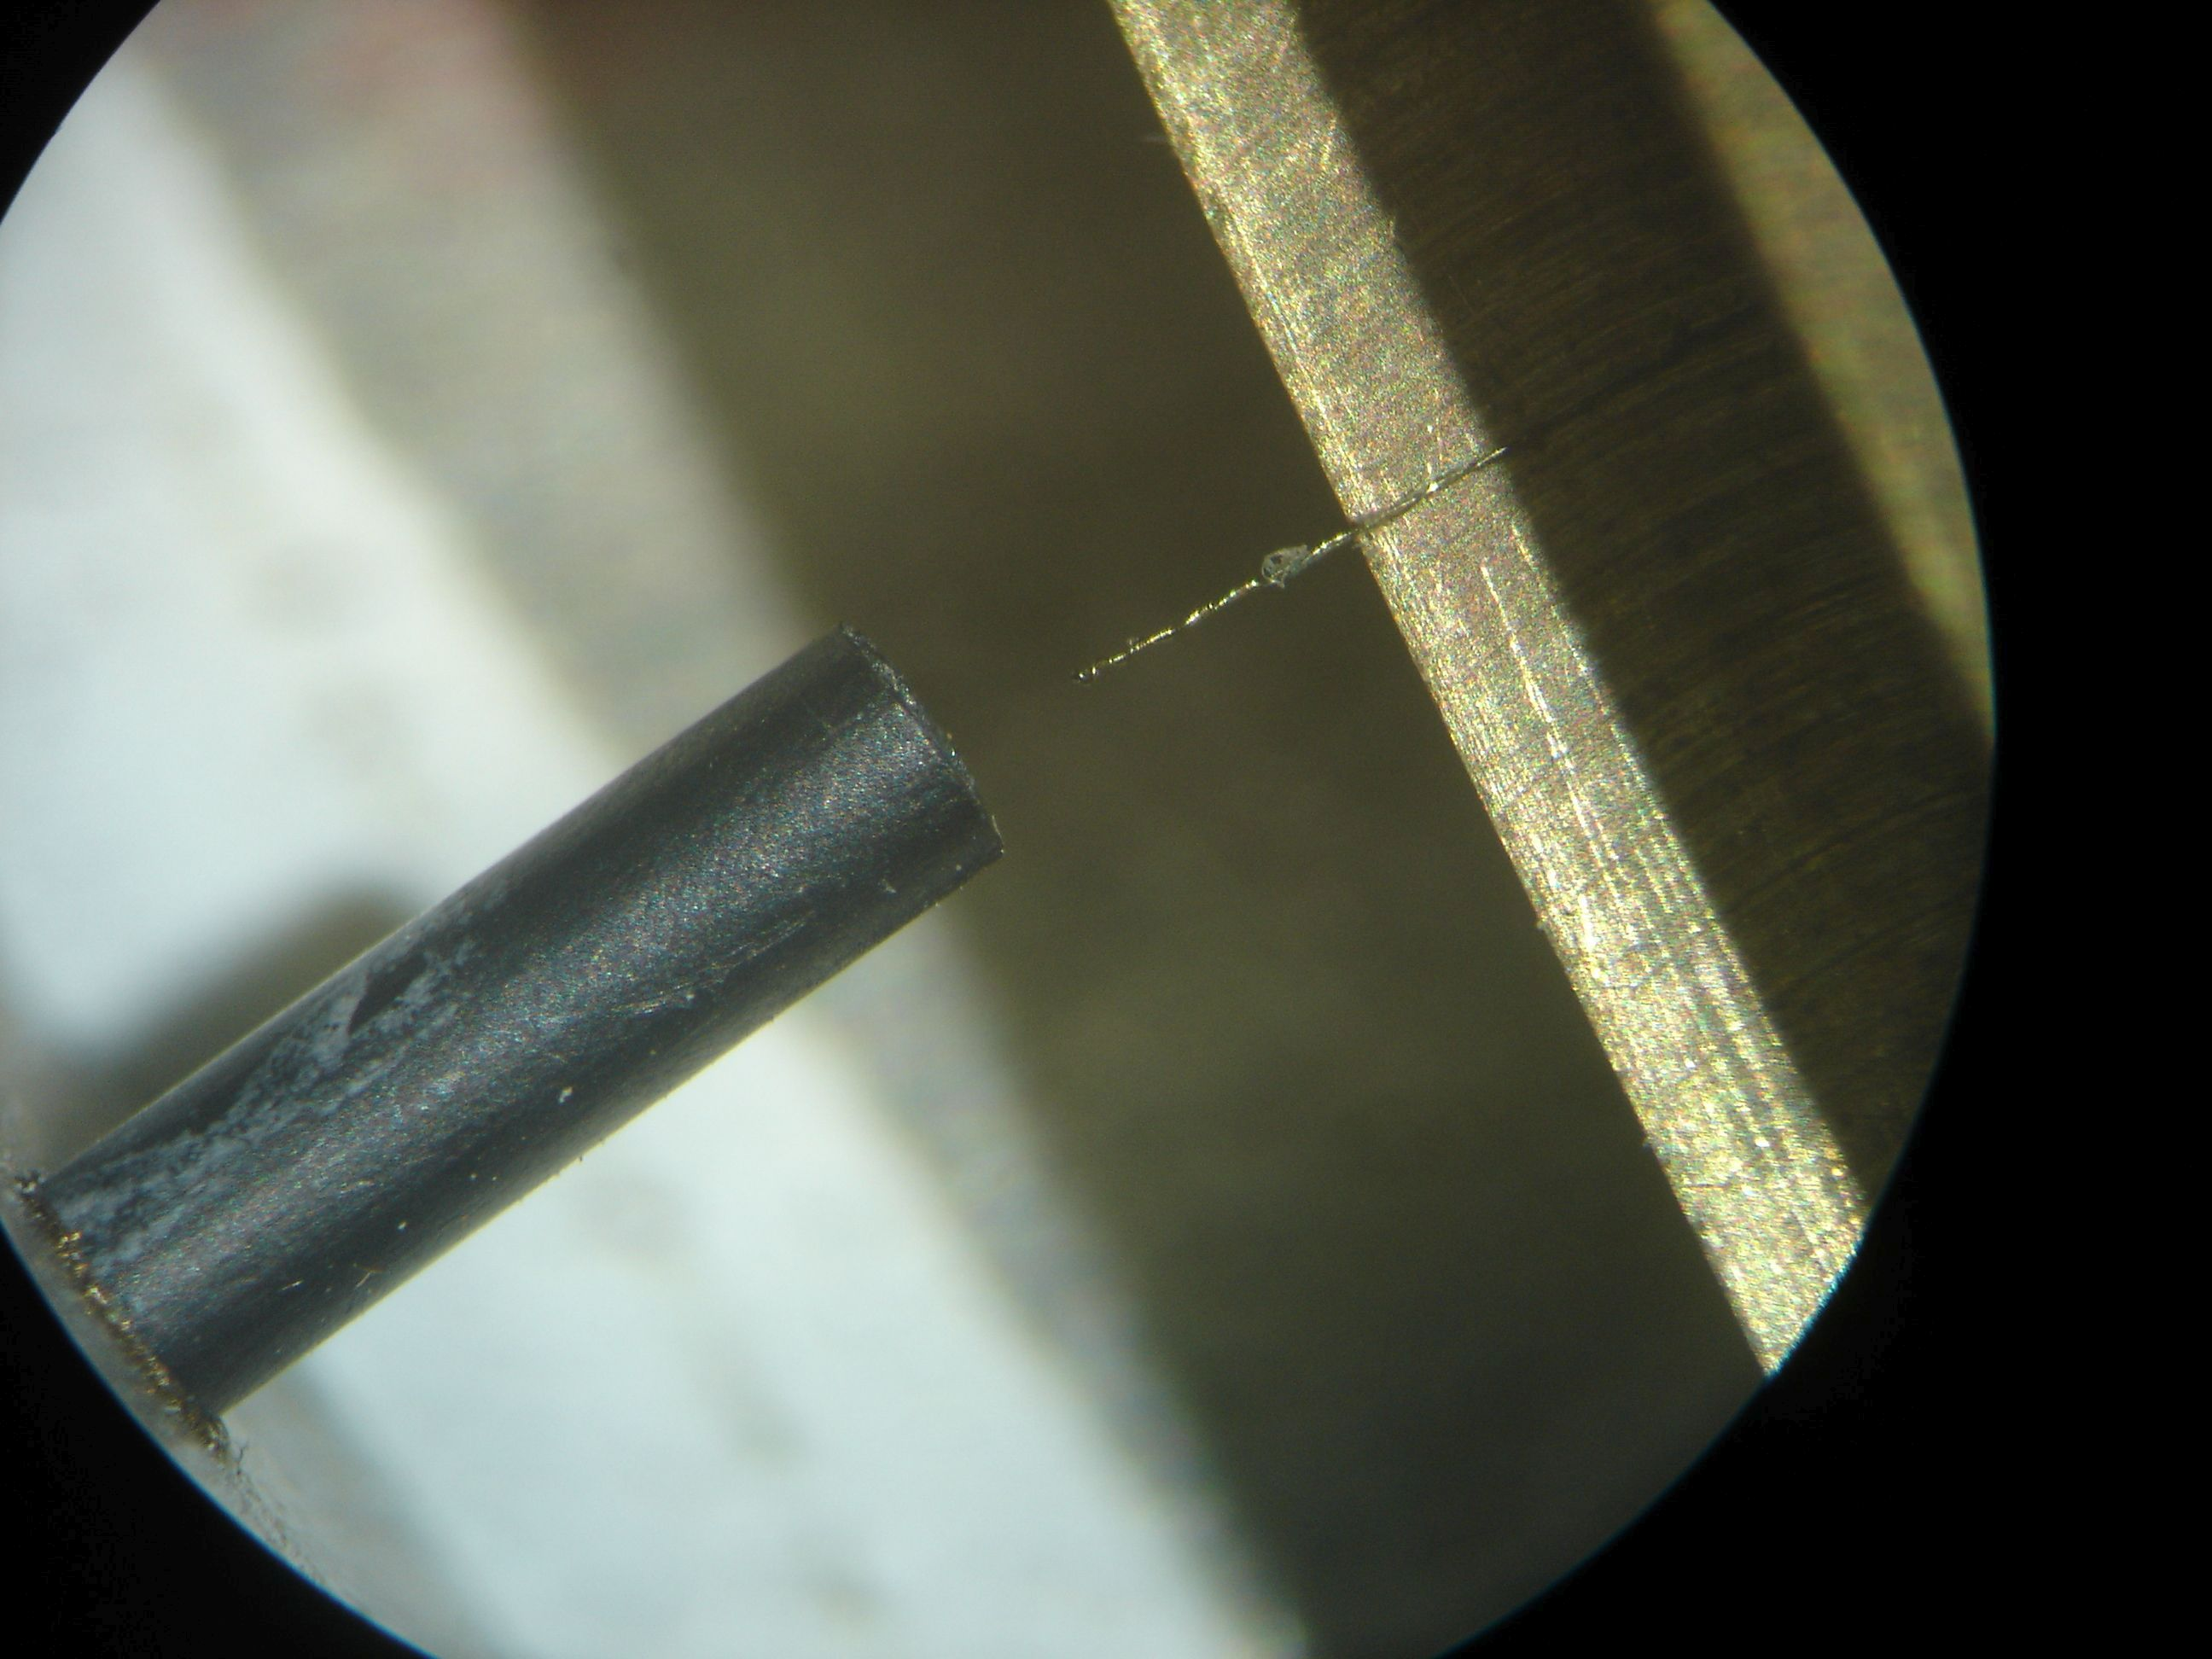
\includegraphics[width=0.5\textwidth]{Figures/WelderMicro.jpg}
	\decoRule
	
\caption[A microphoto of a thermocouple twist ready to be welded.]{A microphoto
of a twisted wire ready to be welded. The black carbon electrode is
\SI{2}{\milli\metre} in diameter.}
	
	\label{fig:TCWeldMicro}
\end{figure}

\subsection{Thermocouple probe construction}

To measure the temperature inside the coaxial heater required the thermocouple
to be inserted into the coaxial heater. For this a fused silica capillary with
an inside diameter of \SI{0.25}{\milli\metre} and an outside diameter of
\SI{0.4}{\milli\metre} was used to construct a probe. (These capillaries were
readily available, in the form of discarded chromatographic columns.) A narrower
capillary was used to draw the wires through the probe capillary, in a process
described in Figure \ref{fig:FineWireThermocouple}. The wires could then be
welded to form a thermocouple, and then drawn to the desired position in the
probe capillary.

\begin{figure}
	\centering
	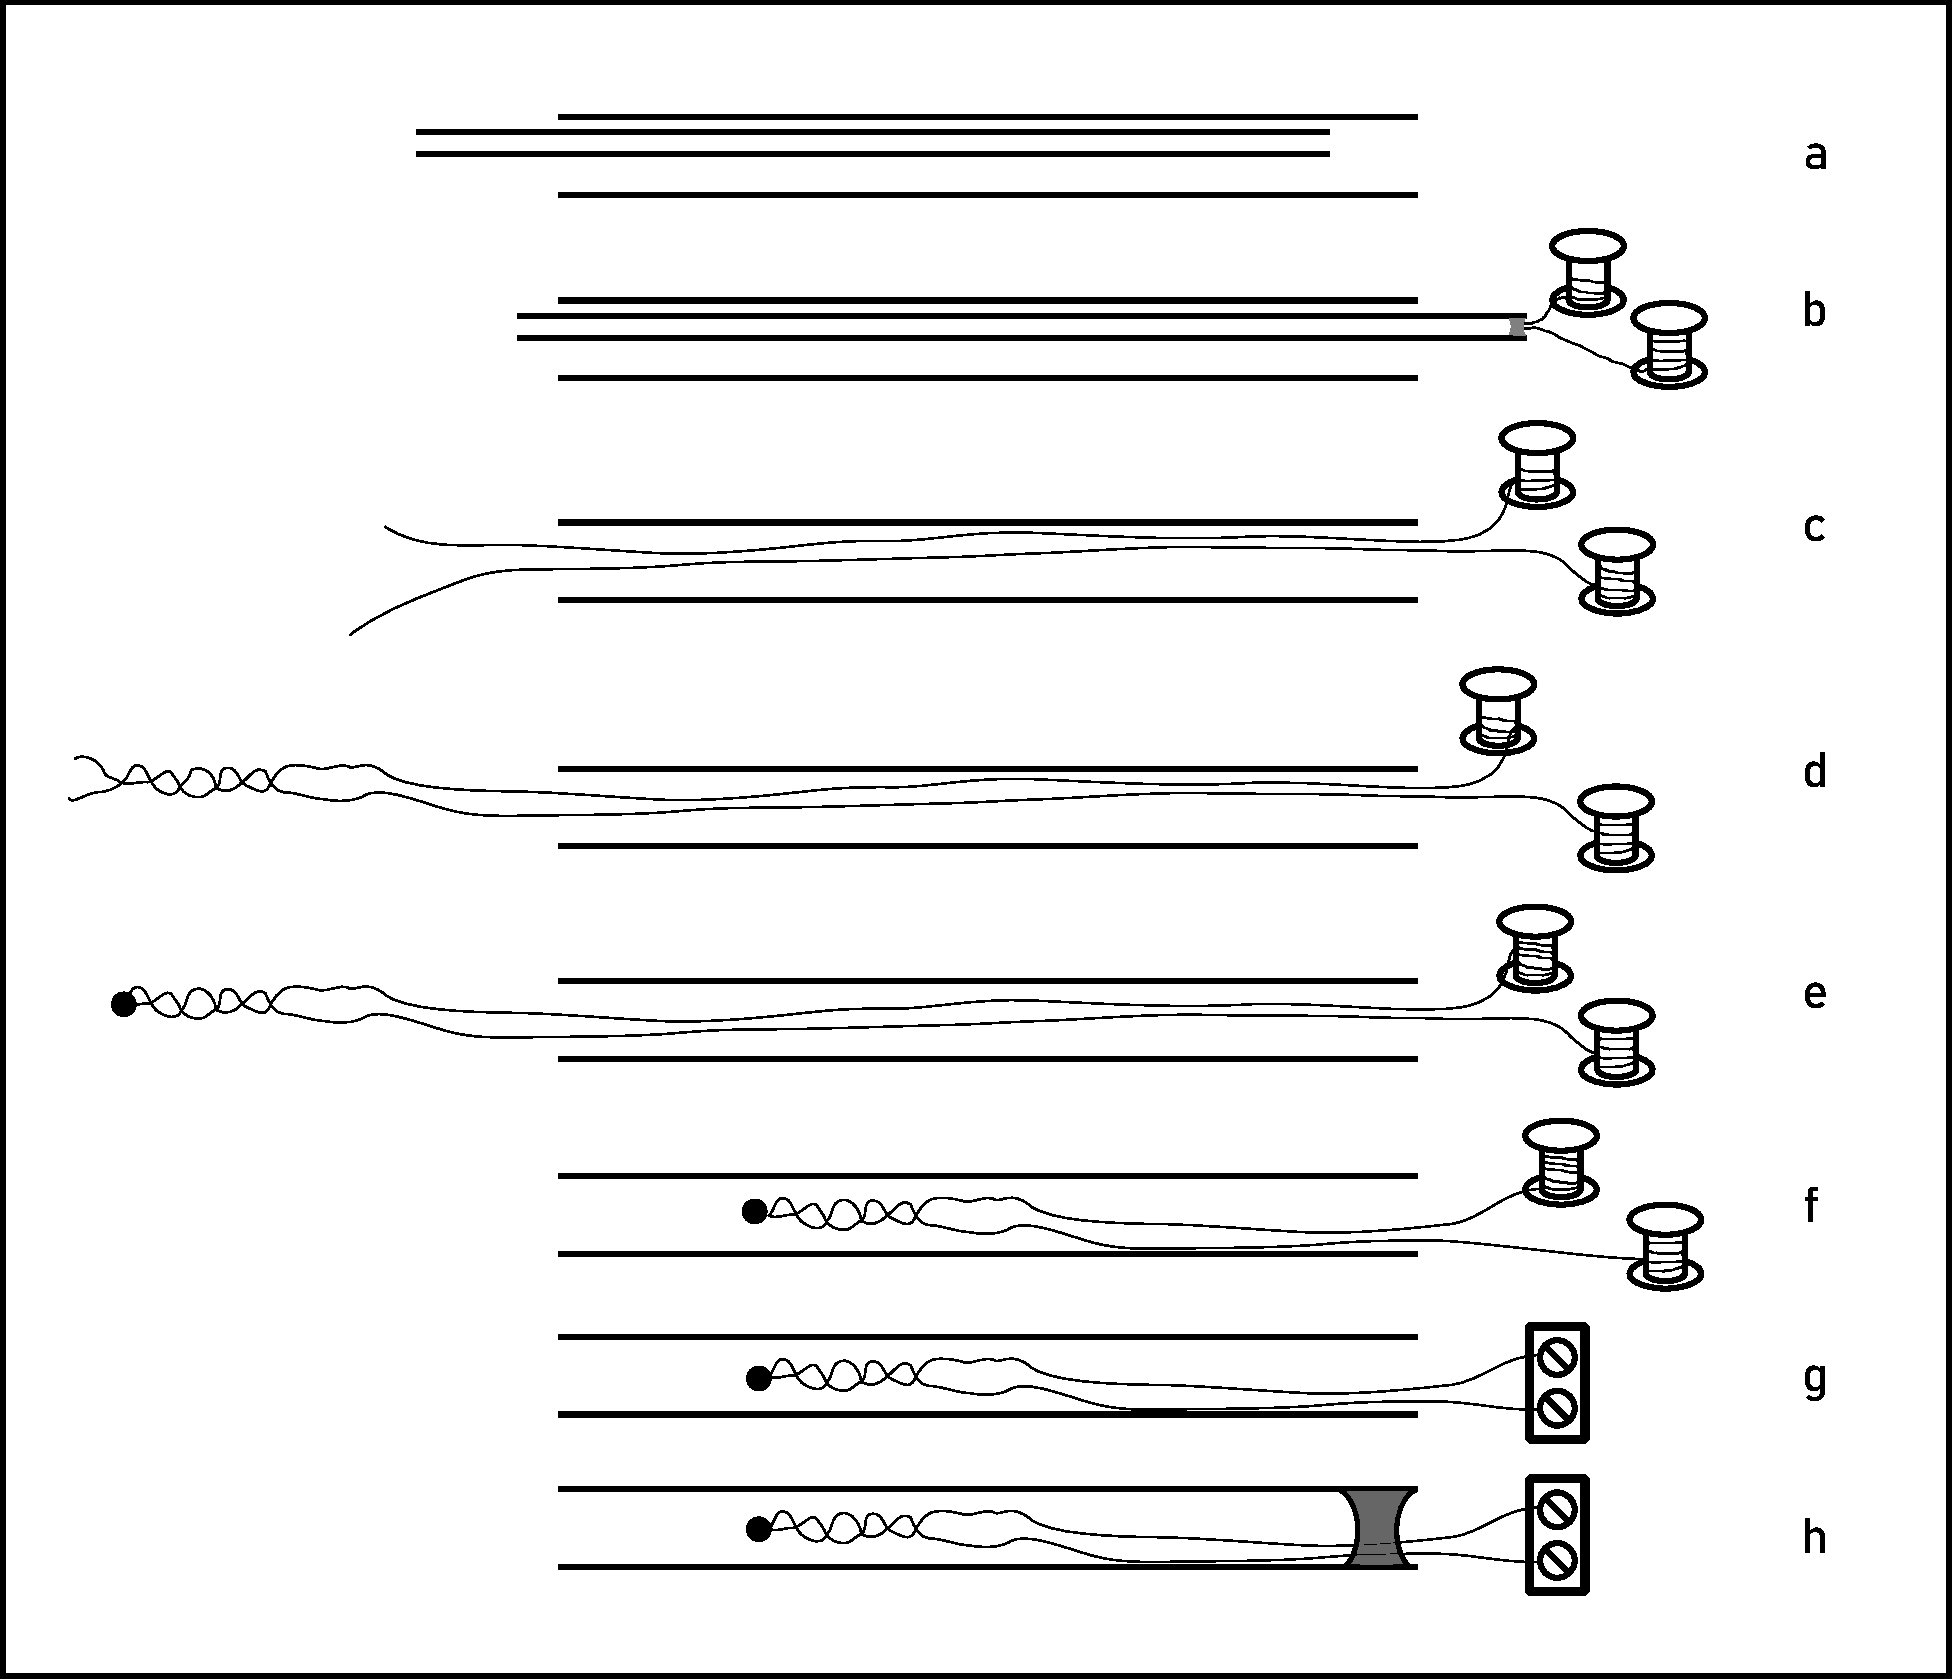
\includegraphics[width=0.8\textwidth]{Figures/FineWireThermocouple.pdf}
	\decoRule
	
\caption[A cartoon explaining how to construct a long, thin thermocouple
probe.]{(a) A narrow capillary is threaded inside a wider one (b) The ends of a
pair of thermocouple wires are fitted inside the end of the narrow capillary and
anchored with cyanoacrylate adhesive. (c) The wires are pulled through the
wider capillary using the narrow capillary. (d) The ends of the wires are twisted
together, creating a mutual mechanical anchor.
(e) The ends of the wires are welded together. (f) The wires are pulled back
into the thick capillary, locating the junction at the desired position in the
capillary. (g) The wires are trimmed and connected to a terminal block. (h) A
drop of cyanoacrylate adhesive is used to anchor the wires permanently in the
capillary. }
	
	\label{fig:FineWireThermocouple}
\end{figure}

\subsection{Thermocouple interfacing}

The Type K thermocouple has a sensitivity of approximately
\SI{41}{\micro\volt\per\celsius}. This means the voltage generated at the
temperature range of interest is too small to be conveniently digitized, and so
needs to be amplified. Because the Type K thermocouple is so commonly used in
industry, amplifiers have been developed specifically for thermocouple signal
conditioning. We chose the AD595 integrated circuit amplifier. The component's
data sheet explains its application concisely: ``The AD595 is a complete
instrumentation amplifier and thermocouple cold junction compensator on a
monolithic chip. It combines an ice point reference with a pre-calibrated
amplifier to produce a high level (10 mV/°C) output directly from a thermocouple
signal.'' \autocite{AD595} The output signal of the AD595 can be directly
digitized for computer recording.

\subsection{Calibration procedure}

The International Vocabulary of Metrology \autocite{JCGM200:2012} define
\keyword{calibration} as ``[an] operation that, under specified conditions, in a
first step, establishes a relation between the \textbf{quantity values} with
\textbf{measurement uncertainties} provided by \textbf{measurement standards}
and corresponding \textbf{indications} with associated measurement uncertainties
and, in a second step, uses this information to establish a relation for
obtaining a \textbf{measurement result} from an indication.''

In the first step of calibration, the \textbf{quantity values} used in the
calibration were the temperature value of the thermocouple probe as provided by
the thermocouple voltage, the AD595 amplifier, the digitization and the
subsequent calculations according to the AD595 data sheet. The
\textbf{measurement standards} were the known responses of the thermocouple
\autocite{Ripple1995}, the amplifier and the digitization system. The
\textbf{indication} was the voltage ratio \(\frac{dV}{Vb}\). As this was a first
attempt a calibration, \textbf{measurement uncertainties} were assumed to be
negligible.

In preparation for calibration the coaxial heater was installed in the oven of
the Varian 3300 GC as it would be when in use. The detector was removed, and the
thermocouple probe was threaded through the detector stem, through the heated
T-piece block, and into the coaxial heater until the thermocouple junction was
about half-way between the inlet end and the detector end of the coaxial heater.
When the system was set up as it would be during use, the coaxial heater was
cooled down, and a power ramp applied. The temperature of the thermocouple was
recorded, together with the voltages \(dV\) and \(Vb\). A curve could then be
plotted of thermocouple temperature \(T_{TC}\) against the voltage ratio \(
\frac{dV}{V_b} \) (Figure \ref{fig:CalibrationCurve}). This revealed the shape
of the function \(T(\frac{dV}{Vb})\), and completed the first step of the
calibration.

\begin{figure}
	\centering
	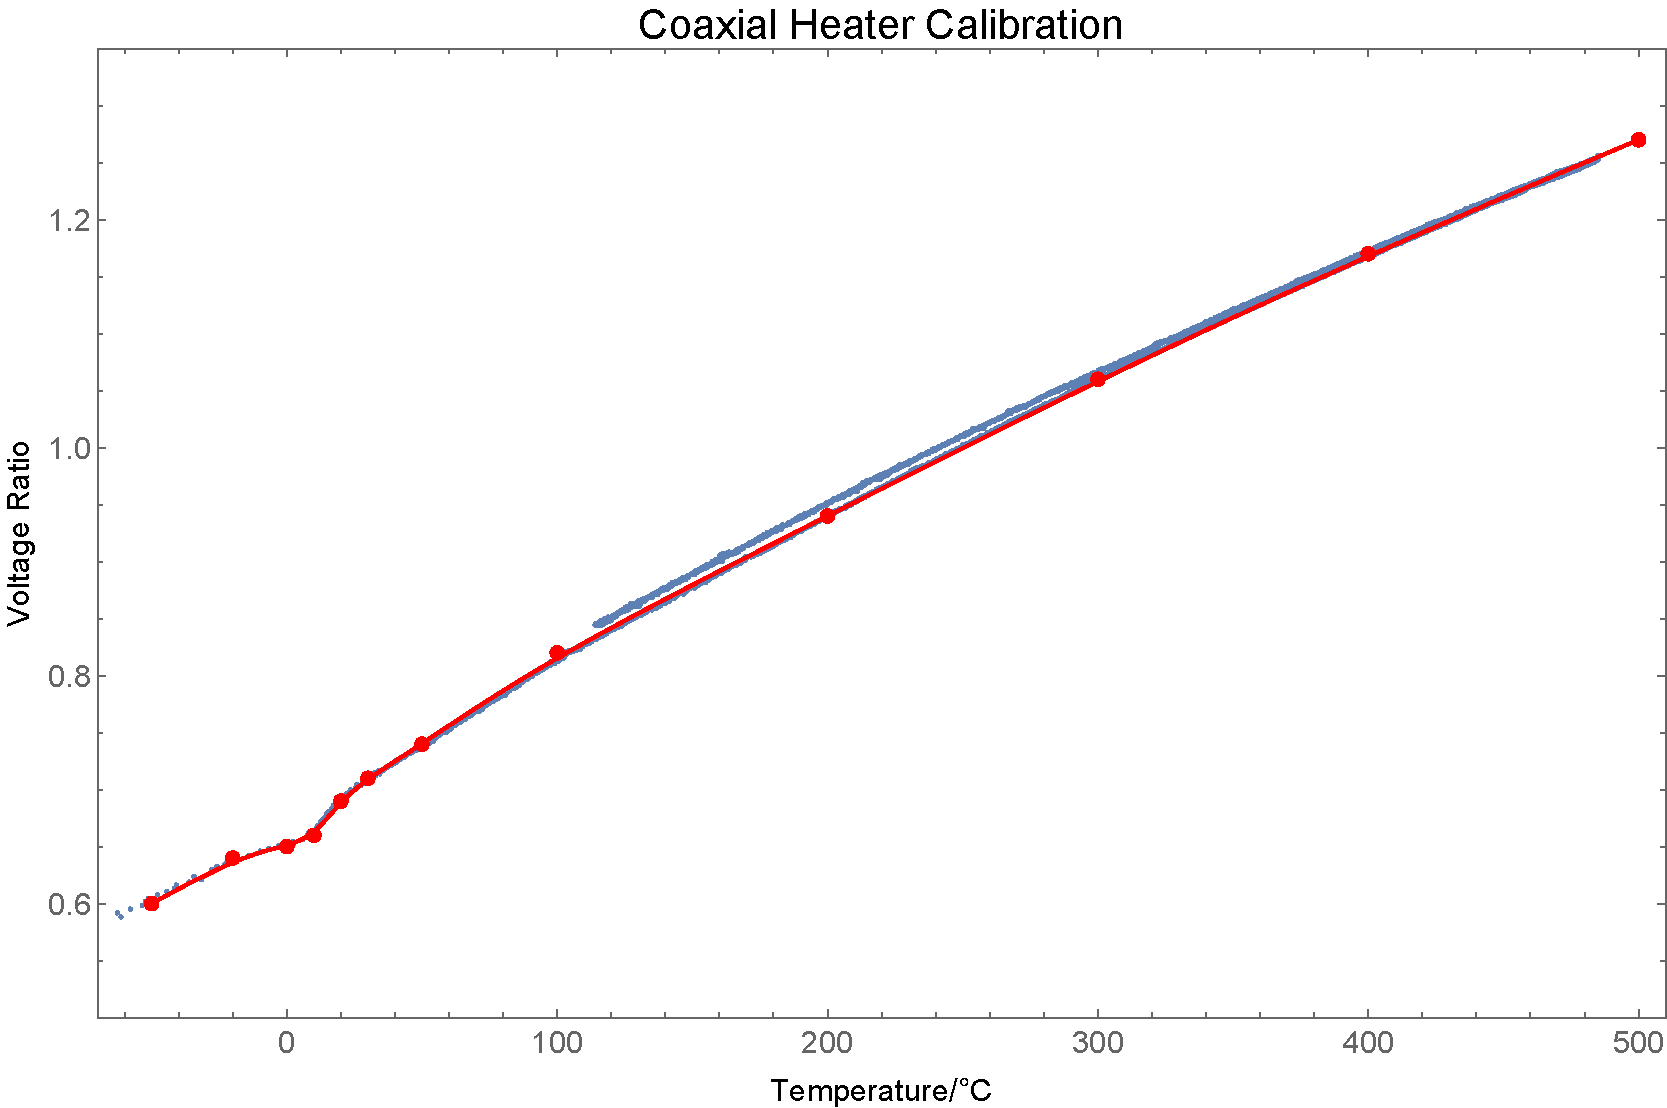
\includegraphics[width=0.8\textwidth]{Figures/2019_07_12_B-spline_fit_CPlot.pdf}
	\decoRule
	\caption[Calibration curve of the coaxial heater]{Calibration curve for the coaxial heater.}	
	\label{fig:CalibrationCurve}
\end{figure}

The second step of a calibration is to establish a \textbf{measurement result}
from an \textbf{indication}. It would be traditional to fit a mathematical
function such as a polynomial to the curve, but a numerical method was chosen
instead. We fitted a B-spline to the curve, and extracted coordinates on the
curve from the B-spline (See Figure \ref{fig:MeasurementCurve}). An
interpolation function was then used to obtain the measurement result \(T\) from
the indication \(dV/V_b\).

\begin{figure}
	\centering
	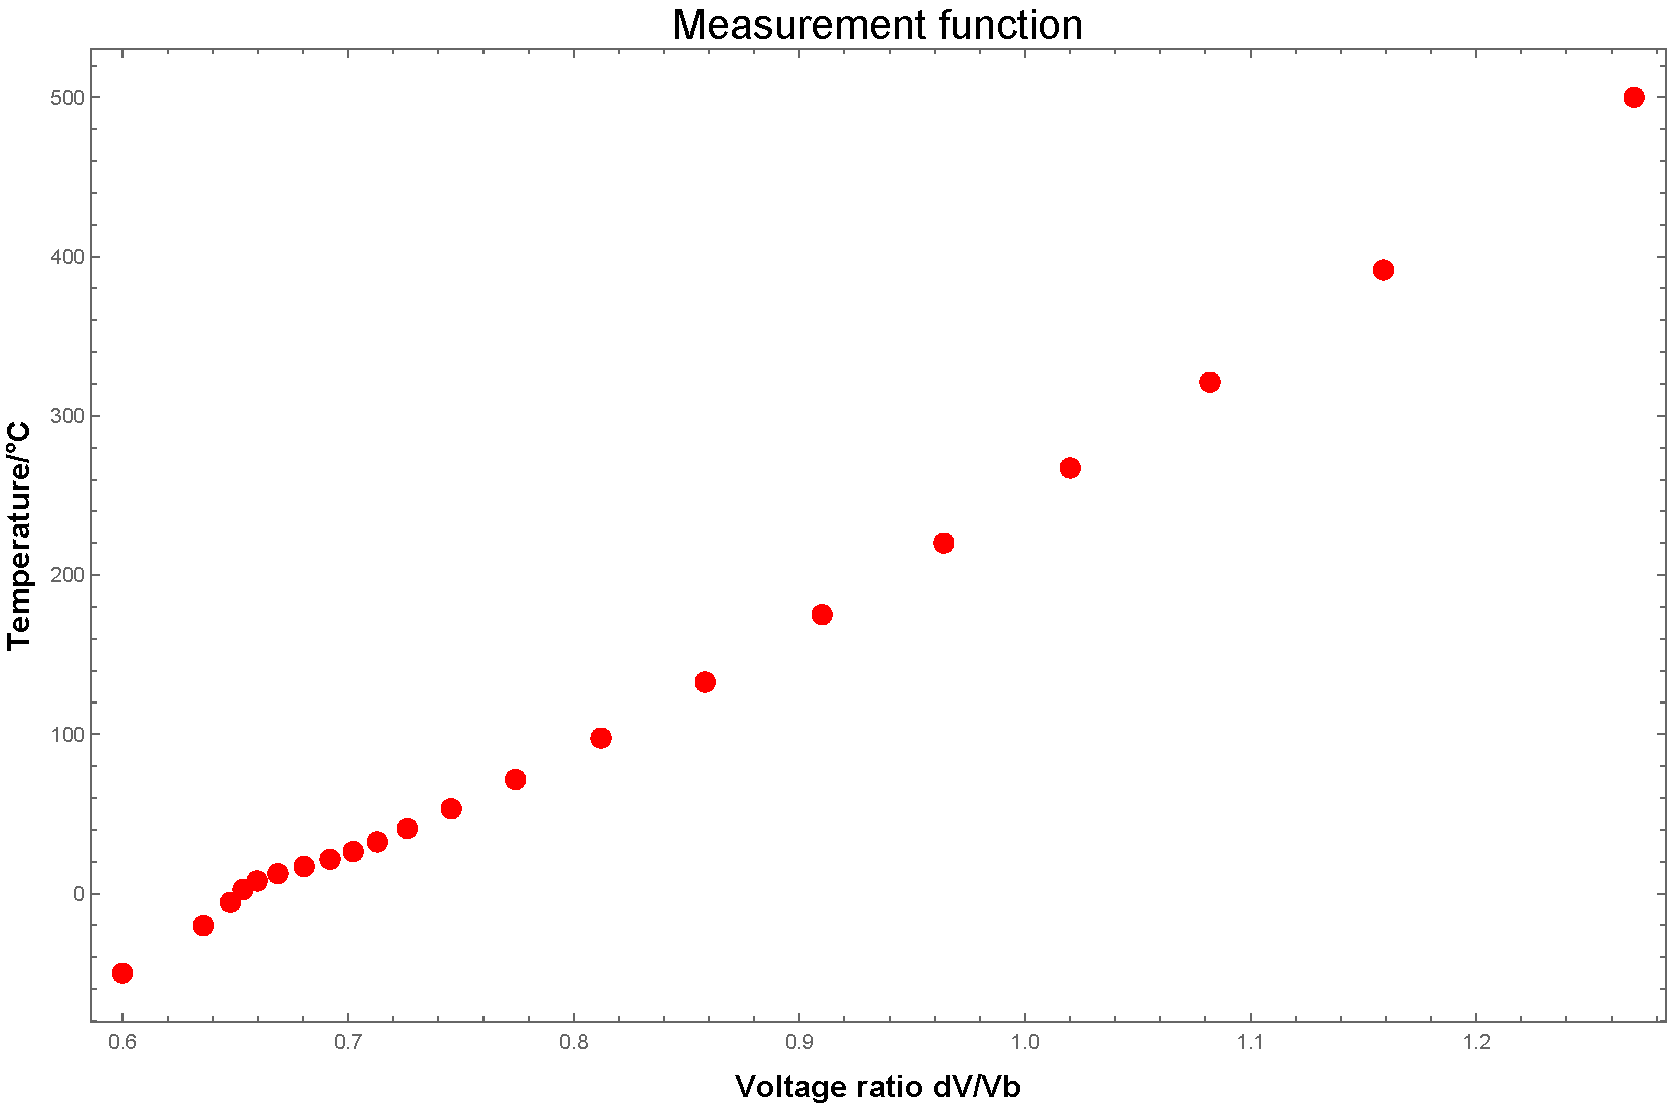
\includegraphics[width=0.8\textwidth]{Figures/2019_07_12_B-spline_fit_PPlot.pdf}
	\decoRule
	\caption[Measurement curve of the coaxial heater]{Measurement curve for the coaxial heater.}	
	\label{fig:MeasurementCurve}
\end{figure}

The calibration could be checked by setting the current through the coaxial
heater to a minimum, at which not enough heat is generated to affect its
temperature. Then the oven of the Varian 3300 GC could be set to a range of
different temperatures. Once equilibrium was reached the reported temperature of
the coaxial heater and the air bath temperature could be compared and the
calibration adjusted.

The technique of constructing a long, thin thermocouple probe allowed the
calibration of the coaxial heater, which makes it possible to translate
chromatographic methods. The probe has also proven useful in other applications,
for example proving overheating in a GC-MS transfer line.

\subsection{Cold spots}
\label{sec:ColdSpots}

For the fastest temperature programming with resistive heating the heating
element should be as light as possible and carry the largest necessary current.
The current doing the heating must be carried to the coaxial heater using a feed
conductor. To prevent the feed conductor from heating up it must have a low
resistance, and this low resistance is achieved by making the conductor as
'thick' or as 'heavy' as necessary, meaning that it is constructed of a material
with a high mass per unit length.

Good electrical metallic conductors are invariably also good thermal conductors,
and therefore, the area around the junction of the feed conductor to the coaxial
heater will always have a lower temperature than the nominal temperature of the
heater. In capillary GC this is undesirable: a cold spot in a column can wreak
havoc with retention times and peak shapes.

Conversely, if an attempt is made to reduce the contact area between the feed
conductor and the thin material of the coaxial heater, a hot spot might develop,
which could burn a hole in the coaxial heater tube or damage the column.

The electrical connection between the feed conductor and the coaxial heater was
therefore designed in the form of an externally heated block. This block was
kept at a higher temperature than the highest expected temperature of the
chromatographic temperature program. This prevented the formation of cold spots
in the coaxial heater, which might lead to cold spots in the column, while also
providing a large contact area so that hot spots do not develop. Each end of the
coaxial heater was fitted into one of two heated blocks, where it was brazed in
place. Each block had a brass tail, to which an electric feed-wire was
soft-soldered. Each block was heated by four \SI{100}{\watt}
Hotset\texttrademark{} electrical cartridge heaters, with dimensions of \SI{6.5
x 40}{\milli\metre}. The cartridge heaters were switched on and off by solid
state relays controlled from the computer. The temperature of the block was
monitored through a thermocouple mounted in a blind hole in the block and the
amount of power to the heaters was controlled by \keyword{pulse width
modulation} (PWM) implemented in software.
 
\subsection{Cold column}
\label{sec:ColdColumn}

In a cold GC stationary phase, the retention factor \(k'\) of a particular
compound can be very high. This means that the analytes migrate slowly relative
to the mobile phase. The lower the temperature, the higher \(k'\) becomes, so
that for very low temperatures the migration of the analyte becomes negligible.
In effect, the analytes are 'trapped'. This trapping, also called
\keyword{cryo-trapping} or \keyword{cryo-focusing} is useful in various aspects
of gas chromatography, such as two-stage thermal desorption or thermal
modulation in GC×GC.

%In one such
%application a programmable temperature vaporizing inlet (PTV) was used to trap
%complex hydrocarbon fractions from an SFC for injecting into a GC×GC system
%\autocite{Potgieter2013}.

In the SFC×GC instrument described here, cryo-trapping was used as the second
stage of a two-stage modulator. (The stop valve described in Section
\ref{sec:stopflow} represents the first stage.) The column was cooled down to
very low temperatures, which trapped any analytes eluting from the first
dimension in a narrow band on the GC column. Once the required amount of
fraction had been collected, the eluate flow from the first dimension was
stopped by closing the stop valve. Then the temperature ramp of the fast GC
would start. As the coaxial heater warmed up the column the values of \(k`\)
would decrease, and the narrow analyte band would start migrating.

The first SFC×GC chromatograph cooled the column by using the oven cryo-cooling
capability of the Varian 3300 GC \autocite{Venter2004, Venter2003}. The purpose
is to cool the GC column to sub-ambient temperatures, normally needed when
analysing volatile compounds. In such cases the \(k'\) values at or near room
temperature are too low to provide adequate retention, and the cryo-cooling
function permits temperature programs to start at sub-ambient temperatures.

The Varian 3300 cryo-cools its oven by injecting liquid carbon dioxide into the
oven's air circulation fan. The evaporating liquid carbon dioxide absorbs energy
from the air, which lowers the temperature of the air in the oven. A control
system controls the amount of carbon dioxide admitted and the amount of heat
added through the oven heaters, thereby keeping the oven at the required
temperature.

The cryo-cooling function can cool down the oven to cryo-trap analytes, but
there are two reasons why it is not suitable for practical trapping in SFC×GC.
The first reason is the quantity of coolant required: doing SFC×GC runs revealed
that about \SI{15}{\kilogram} of carbon dioxide was consumed per run. A standard
cylinder of carbon dioxide contains \SI{33}{\kilogram}, which implies that a new
cylinder would be required every two runs. Such a rate of use is much too high
for the intended application of the instrument. The second reason using is that
it is much too slow. The time spent on cooling the oven and the column is time
that cannot be spent doing separations, and cooling a conventional GC oven takes
a lot of time: the Varian 3300's cryo-cooling function took \SI{30}{\second} to
cool the column down to a low starting temperature. A commercial
forced-convection system (``GC Chaser'' supplied by Zip Scientific) improves the
cool down time of an Agilent 6890 GC oven, taking 7 minutes instead of 16,
cooling down the oven from \SI{350}{\celsius} to \SI{30}{\celsius}.
Cooling the column in an air bath has the same drawbacks of low conductivity and
low heat capacity as air-bath heating has (see Section \ref{sec:RampRates}).

A system was therefore developed that injected liquid carbon dioxide into one
end of the space between the column and its coaxial heater, with the other end
open to the atmosphere. When the valve opens the space rapidly fills with liquid
carbon dioxide, while the pressure drops from \SI{55}{atm} in the cylinder to
\SI{1}{atm} at the outlet. The liquid boils, absorbing large quantities of heat
from the column and coaxial heater in the process, so that their temperatures
decrease rapidly. This system solves the speed and coolant consumption problems:
because the coolant is in direct contact with the parts that need to be cooled,
the cooling is rapid, and because the coolant is applied where it is needed,
only a small quantity is required.

The carbon dioxide for cooling the coaxial heater was introduced through the
same heated block that provided the electrical connection. (See Section
\ref{sec:ColdSpots}.) A T-piece design allowed the liquid carbon dioxide to be
admitted to the end of the coaxial heater, which was brazed to the block. A
micro-union brazed to the block sealed the column's exit port, and the liquid
carbon dioxide entered along the side of the T (Figure \ref{fig:ManifoldDims}
and Figure \ref{fig:ManifoldAssy}). A metering valve allowed the flow rate of
the coolant to be adjusted, and a computer-controlled solenoid valve switched
the flow on or off.

\subsubsection{Cryogen supply}

The carbon dioxide for cooling was supplied by Afrox, in high-pressure
cylinders each containing 33kg of technical grade carbon dioxide. Each cylinder
was internally equipped with a \keyword{dip tube}, a tube that extends from the
valve at the top of the cylinder to the bottom of the cylinder. This ensures
that when the valve is opened, liquid carbon dioxide is delivered.

Experience taught that for repeatable cooling, the source of liquid carbon
dioxide had to be near the solenoid valve. If this was not the case, when the
valve was opened initially only carbon dioxide gas would be admitted, followed
by a mixture of gas and liquid, and only finally liquid. (This is similar to the
common experience of opening a water tap after a municipal water supply
interruption: a lot of gurgling and spitting before a reliable stream of water
flows from the tap.) Such unreliable coolant flow gives unreliable cooling.
To solve this problem we installed a reservoir for liquid carbon dioxide on top
of the GC. The problem of filling a receptacle with liquid carbon dioxide was
described in Section \ref{sec:CO2Pump}, so the final design of the reservoir
took the form of a coil of copper tube immersed in a circulating coolant (Figure
\ref{fig:CryogenReservoir}). Mounting the reservoir above the cut-off valve
allows the liquid to collect at the bottom and allow gas to collect at the top,
so that when the valve opens the flow into the coaxial heater contains only
liquid.

\subsection{Column mounting}

The T-piece blocks described in Section \ref{sec:ColdSpots} and Section
\ref{sec:ColdColumn} above and also depicted in Figure \ref{fig:ManifoldAssy}) acted as electrical
connections for the coaxial heater and as injection point for coolant. The block
is heavy compared to the coaxial heater and column, and also has to absorb the
forces of the coolant inlet tube and the electrical connections. The column runs
from the heated inlet/detector to a heated T-piece block, and in between it
should not be exposed to any low-temperature cold spots, therefore the gap
between the T-piece block and the inlet/detector should be quite small, but the
gap cannot be zero, because electrical isolation needs to be maintained.
Also, fused-silica capillary columns are fragile and misalignment causes them to
break. Therefore, mechanically stiff and accurate mounting was needed for the
T-piece blocks, to allow the precise but adjustable alignment of the T-piece
blocks with the inlet/detector.

The final design for mounting the T-piece blocks was a pair of parallel rails.
These rails were held in place in the Varian 3300 oven by friction, so that they
could be adjusted and removed as necessary, yet were stiff enough to transfer
the necessary forces without deflecting. The pointed ends of the rails pressed
against a solid aluminium plate used as the floor of the oven, and at the top
adjustable points pressed against pressure plates which pressed against the roof
of the oven. Figure \ref{fig:RailsDrawing} shows a technical drawing of the
rails as designed.

The T-piece blocks were the electrical connections for the resistive coaxial
heater, which meant they needed to be electrically isolated, but they were also
heated, which meant that the insulation had to be resistant to heat. A
commercially available material that met these requirements was found in the
form of \keyword{silicon mica}, a composite material of mica and a silicone
resin. This material has a continuous operating temperature of at least
\SI{500}{\celsius}, making it ideally suited to GC applications. The silicon
mica is also machinable and can easily be shaped to the required design. 

The T-piece blocks were mounted on a pair of cars riding on the round-bar rails.
Each car was designed as a sandwich of plates of stainless steel and silicon
mica around a pair of brass bushes. Once assembled, the cars offered a set of
studs on to which the user could fit and bolt down the T-piece blocks. The
positions of the cars were determined by a locking collar on one of the rails.
Figure \ref{fig:CarsDrawing1} shows technical drawings of the cars that explains
the design.


\subsection{Heating control}

The amount of electrical power supplied to the coaxial heater was controlled by
a bank of six PNP 2N2955 transistors, connected in parallel to distribute their
heat dissipation. The final control signal was a voltage set either by a
potentiometer from the front panel, or by the computer. An operational amplifier
adjusted the current through the coaxial heater circuit so that a portion of the
voltage applied to the coaxial heater was equal to the set-point voltage. By
varying the set-point voltage the current through the coaxial heater can be
controlled to provide any desired amount of heat (\(P = I^2R\)).

\subsubsection{Temperature monitoring}

Independent of the amount of power dissipated in the coaxial heater, the current
through the reference resistor was compared to the current through the column.
This ratio corresponds to the resistance of the coaxial heater. This resistance
is a function of the temperature of the heater. Through the calibration
procedure described above the temperature of the coaxial heater can be
calculated. The computer can do this fast enough so that a temperature
measurement is available to continuously feed to a control system.

\subsubsection{PID tuning}

A proportional-integral-derivative (PID) controller was used to calculate the
amount of power necessary to keep the temperature of the coaxial heater as close
to the temperature set point as possible. The temperature set-point, in turn,
was given by the desired chromatographic temperature ramp.

The process of determining the best calculation by the PID is called
\keyword{tuning}, and usually consists of determining the optimum values of a few
parameters. Tuning PID controllers is a complex sub-discipline of process
engineering, and outside the scope of this project, but for practical purposes
we used a privately published step-by-step tuning method \autocite{Peacock2008}
which is a version of the Cohen-Coon tuning method.

Figure \ref{fig:LoopTuning} shows the effect of an improved loop tuning. 

\begin{figure}
	\centering
	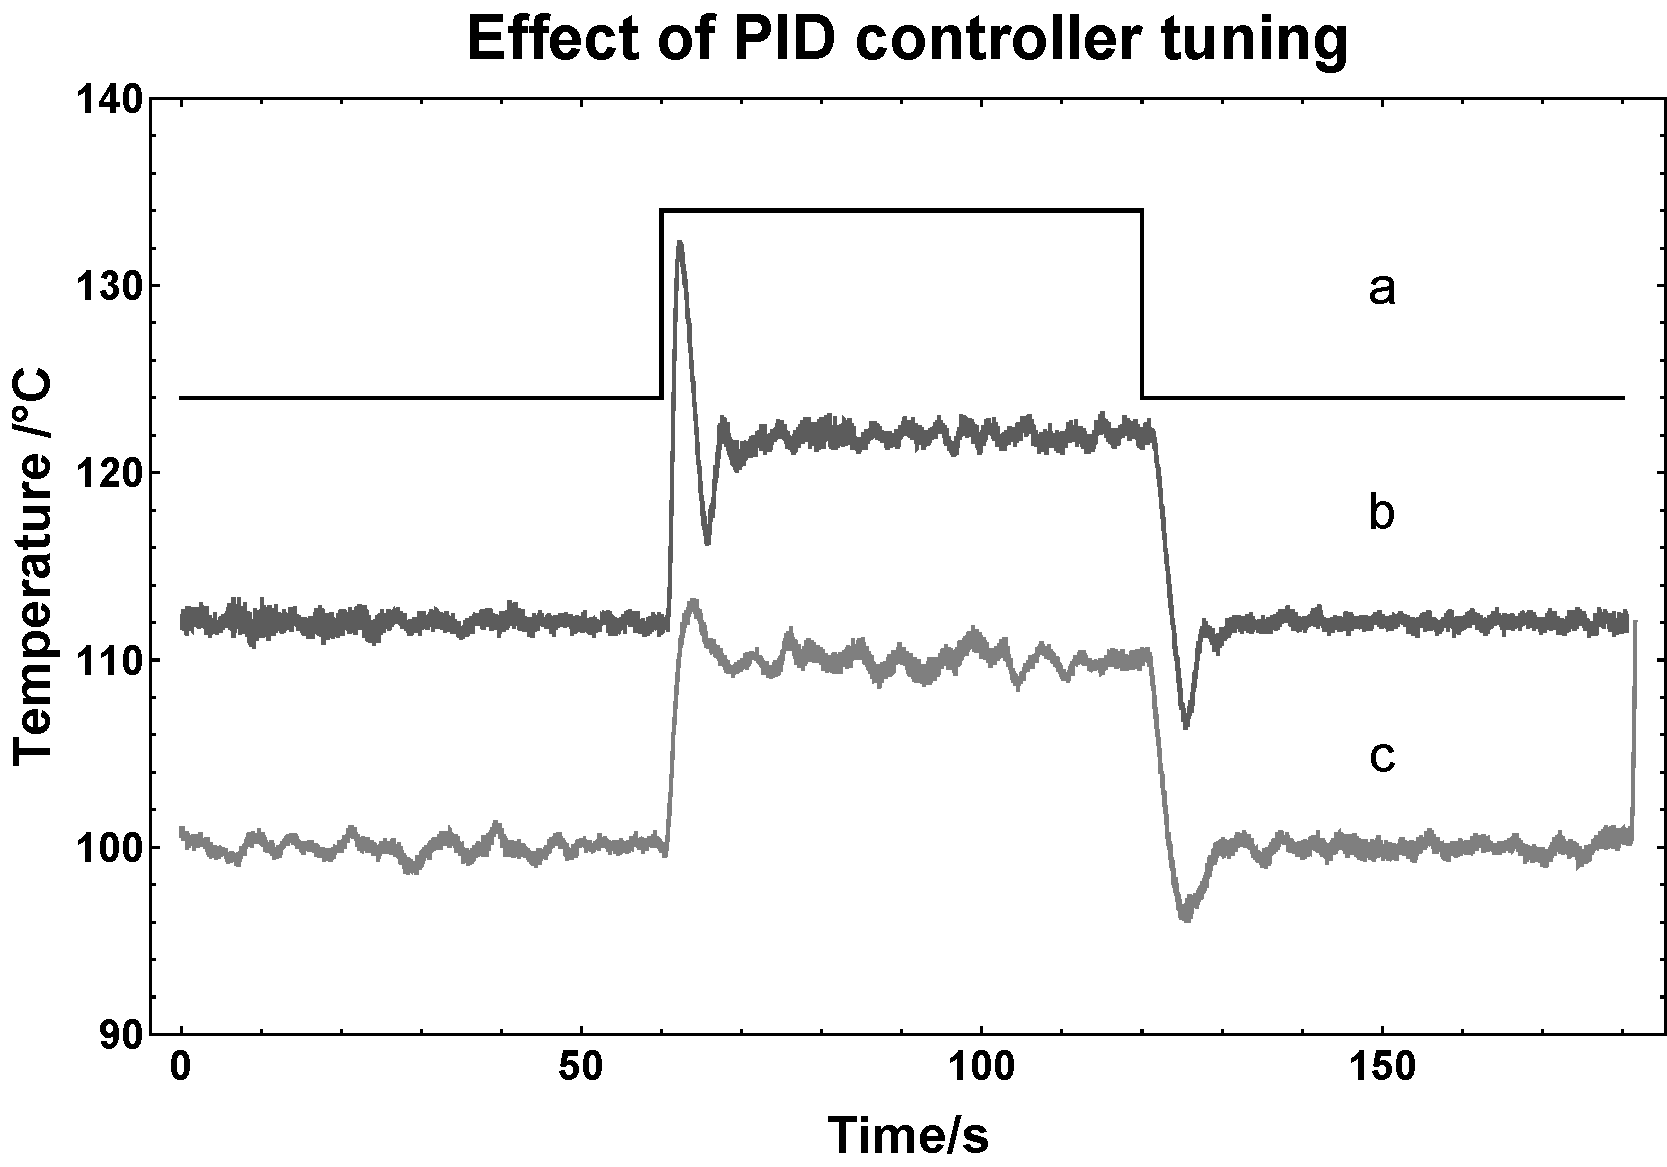
\includegraphics[width=0.8\textwidth]{Figures/LoopTuningGraph.pdf}
	\decoRule	
	\caption[Effect of controller tuning]{An illustration of effective PID
	controller tuning. The trace (a) represents the set point change over time and
	includes a step change. (b) Before tuning the temperature overshoots and then
	undershoots the step change in the set point. (c) After the controller has been
	tuned the overshoot in response to a step change in the set point is minimized. }
	\label{fig:LoopTuning} 
\end{figure}

A properly tuned heater helps to improve the repeatability of the chromatography
through reliable temperature programs and prevents damage to the column due
overheating during set point overshoots.

\subsubsection{Heating rates}

As discussed in Section \ref{sec:RampRates}, for fast temperature-programmed gas
chromatography the ramp rate needs to be in the order of thousands of degrees
Celsius per minute.

\begin{figure}
	\centering
	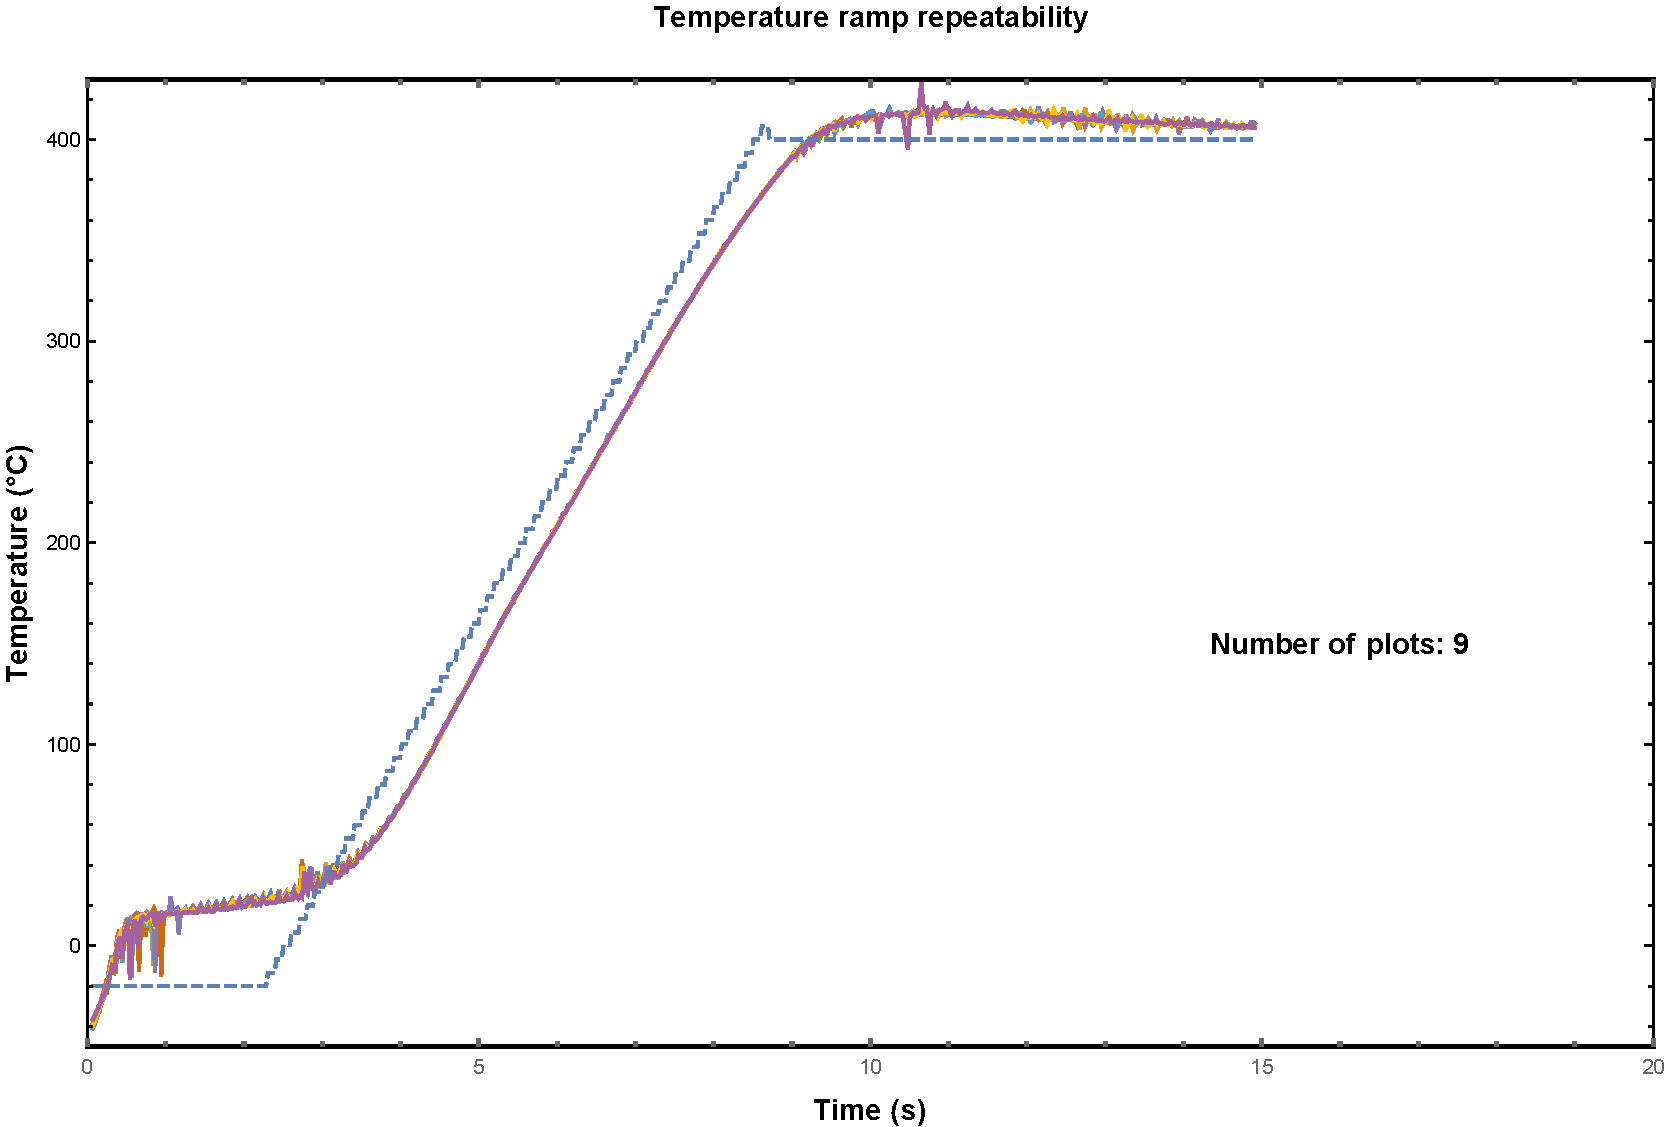
\includegraphics[width=0.8\textwidth]{Figures/high_rate_heating.pdf}
	\decoRule
		
	\caption[Heating rate illustration]{A graph of 9 identical, consecutive
	temperature ramps overlaid. The heating rate is \SI{4000}{C\degree\per\minute}.
	The temperature follows the set point faithfully up to \SI{350}{\celsius}.}

	\label{fig:4000K/min} 
\end{figure}

Figure \ref{fig:4000K/min} contains heating ramps executed by the coaxial
heater. The heating rate was \SI{4000}{\celsius\per\minute}, and there are no
significant differences between the 9 consecutive ramps.

\subsubsection{Cooling rates}

The project did not demand a precise knowledge of, or control over, the cooling
rate of the coaxial heater. The only requirement was that cooling should be as
fast as possible. The cooling rate could be adjusted through the metering valve,
and an optimum cooling rate of \SI{5100}{C\degree\per\min} was achieved with a
carbon dioxide flow rate of around \SI{30}{\gram\per\min}. This allowed the
column to be cooled down from \SI{350}{\celsius} to \SI{-20}{\celsius} in about
2 seconds. At this rate the portion of the chromatographic cycle that is not
used for separation is dominated by fraction collection, and further cooling
rate increases will not significantly reduce sample throughput.

\section{Detector}

The detector used in this fast GC was an unmodified Varian\texttrademark{} 3300
flame ionization detector (FID). The detector bias voltage was supplied by the
original electronics, but a stand-alone high-speed electrometer (V.G. Micromass
Ltd, Model M406-H) captured the signal, which was then conditioned by a
bench-top amplifier (V.G. Micromass Ltd, Model M406) before it was sent to the
computer. This electrometer and amplifier were fast enough to detect and amplify
the signals generated by the fast GC.

\section{Data acquisition and control software}

The whole SFC×GC instrument was controlled from a single PC, running a single
program. The program was written in LabVIEW 7.1\texttrademark{} (National
Instruments). This software was designed to interact very easily with the
National Instruments PCI-6014 multifunction data acquisition board.

LabVIEW is a \keyword{visual programming language}, so called because programs
are created by manipulating icons and wires on a screen, instead of typing text.
This visual aspect of it makes it very easy to develop user interfaces as
\keyword{virtual instruments} and get quick results. Figure \ref{fig:SFCGCFastVI}
shows the interface of the program used to control the SFC×GC instrument.

\begin{figure}
	\centering
	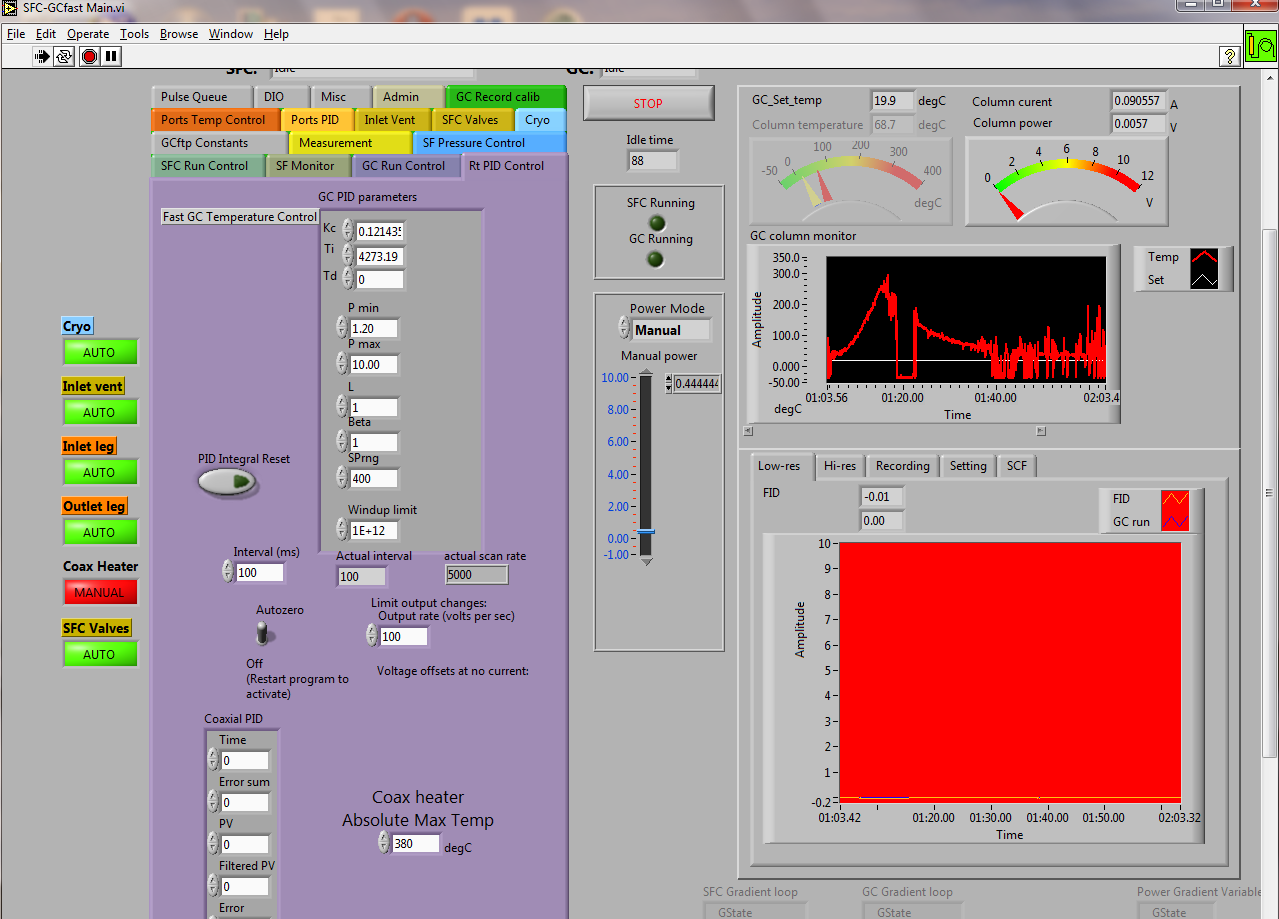
\includegraphics[width=0.8\textwidth]{Figures/Screenshot.png}
	\decoRule
	
	\caption[The main LabVIEW VI]{A screenshot of the LabVIEW virtual instrument
	used to control the SFC×GC instrument.}
	
	\label{fig:SFCGCFastVI}
\end{figure}


\section{Data structure}

In GC×GC, 2D data is recorded as a continuous FID output stream --- as if it is
a 1D GC chromatogram --- and later converted into a 2D chromatogram using
knowledge of the modulation period. For two reasons we could not use this
approach. First, in our instrument the first (SFC) dimension runs in a
stop-flow mode making continuous data recording inappropriate. Second, the
duration of the cooling cycle varies, which would introduce unacceptable
variation in \textsuperscript{2}D retention times.

We therefore constructed 2D chromatograms by recording a GC run for each SFC
fraction injected. The \textsuperscript{1}D
retention times were recorded as the start times of each individual GC run.
The \textsuperscript{2}D retention times were measured from
the time the GC fast temperature program started. 

\section{Data visualization}
For data visualization we used the technical computing system Wolfram
Mathematica 11.3\texttrademark{}. Mathematica is an extremely powerful and broad
system, and we found it useful for its data manipulation and visualization
tools.

The collected data could be handled in different ways. One way was to split it
up into separate GC runs. Each individual GC run and its associated data could
then be examined using the \texttt{Manipulate[]} function (Figure
\ref{fig:SingleGC}).

\begin{figure}
	\centering
	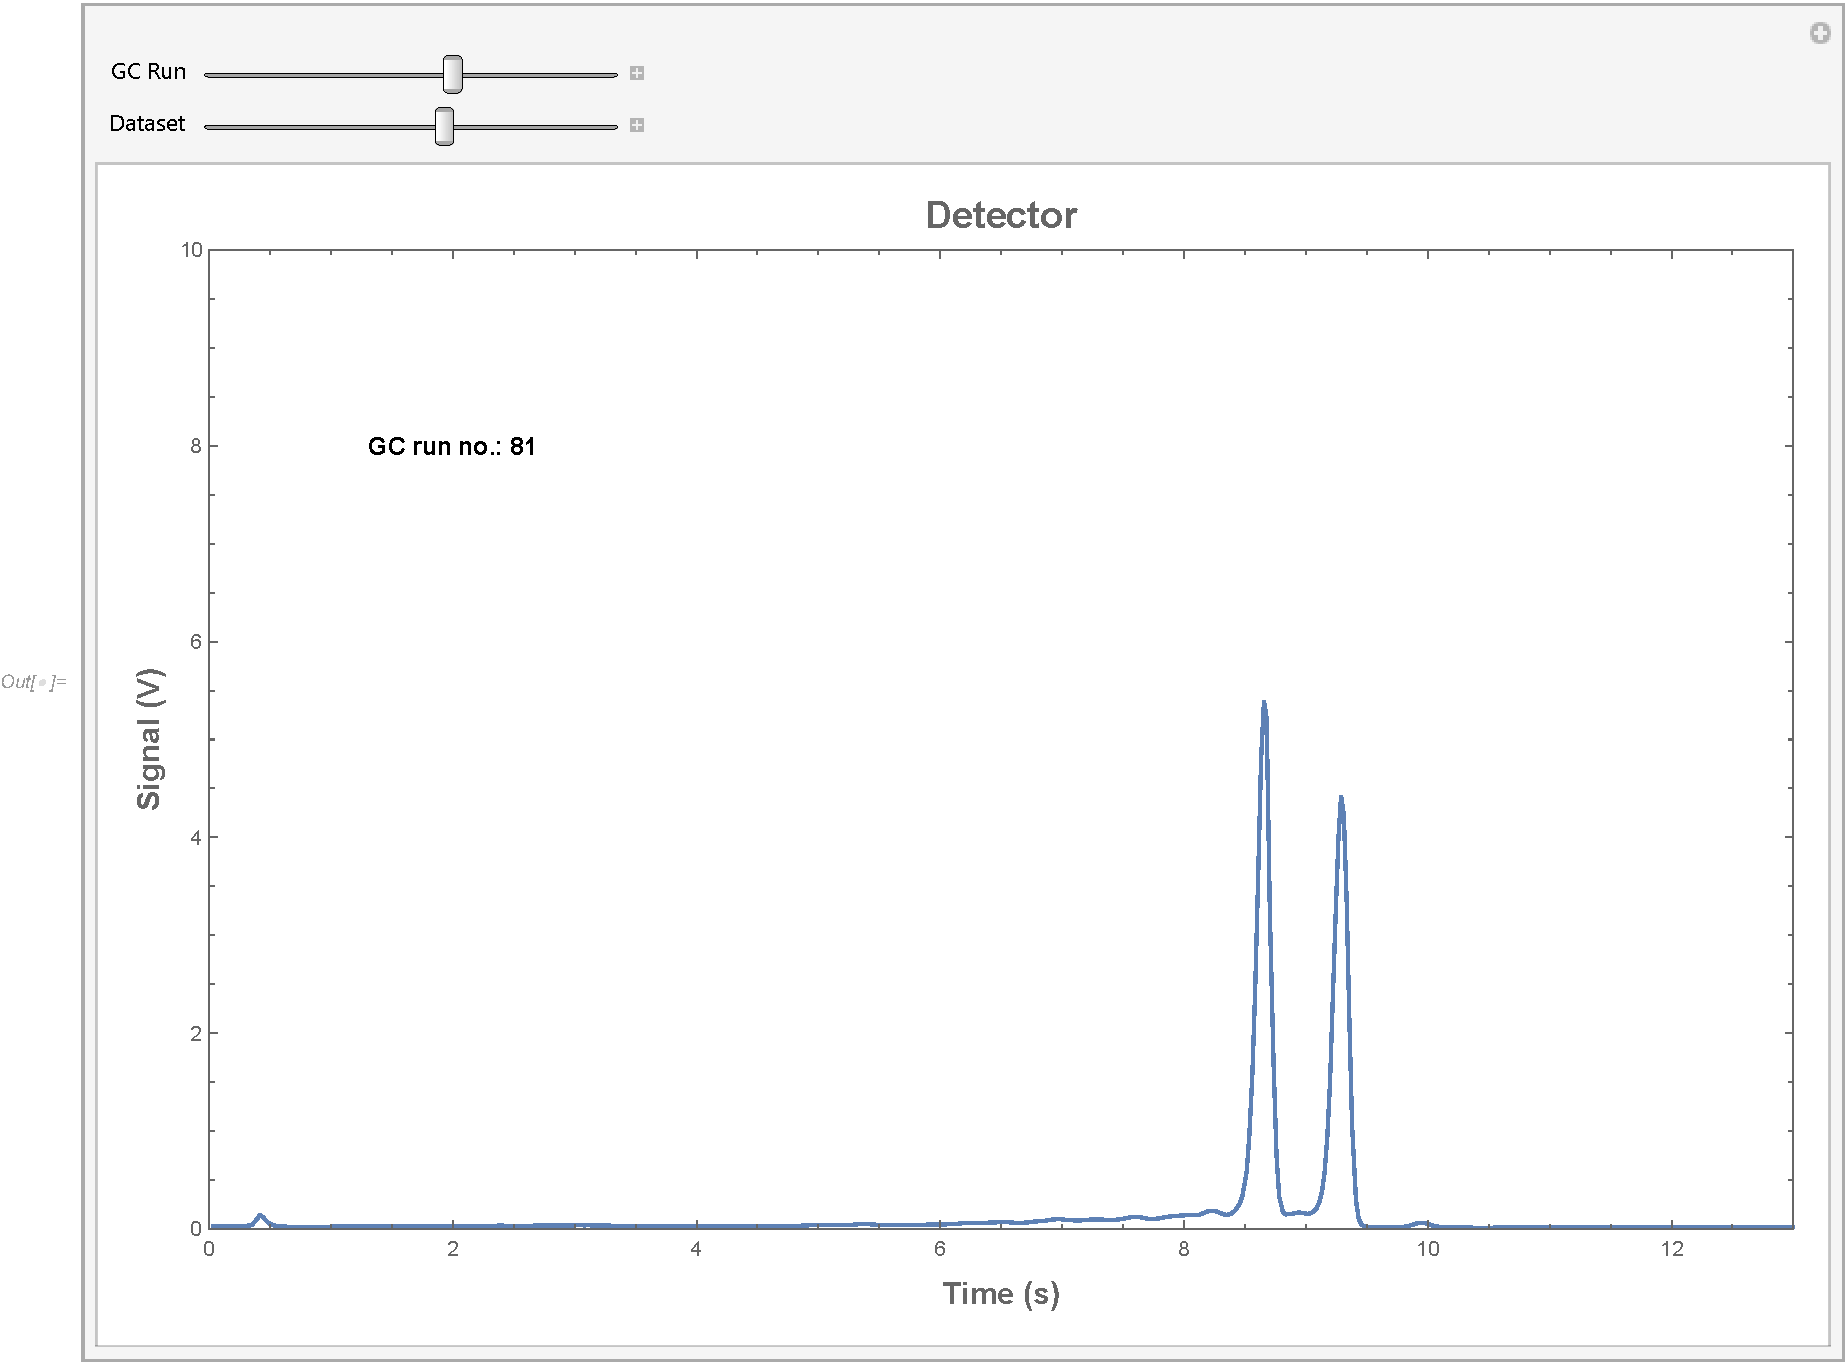
\includegraphics[width=0.8\textwidth]{Figures/Manipulate.pdf}
	\decoRule
	
	\caption[A single fast GC chromatogram ]{A single fast GC chromatogram, in a
	Mathematica \texttt{Manipulate[]} environment. The sliders can be used to select
	the which GC run to view, and which data of that run. }
	
	\label{fig:SingleGC}
\end{figure}

Then the data could be re-arranged into a list of three-element lists, with
$^1$D retention time, $^2$D retention time, and detector signal as the elements
of the inner lists. The Mathematica functions \texttt{List3DPlot[]} and
\texttt{ContourPlot[]} could then be used to plot 3D chromatograms (Figure
\ref{fig:2DChromatogram}) or contour plots (Figure \ref{fig:Contourplot})
respectively.

\begin{figure}
	\centering
	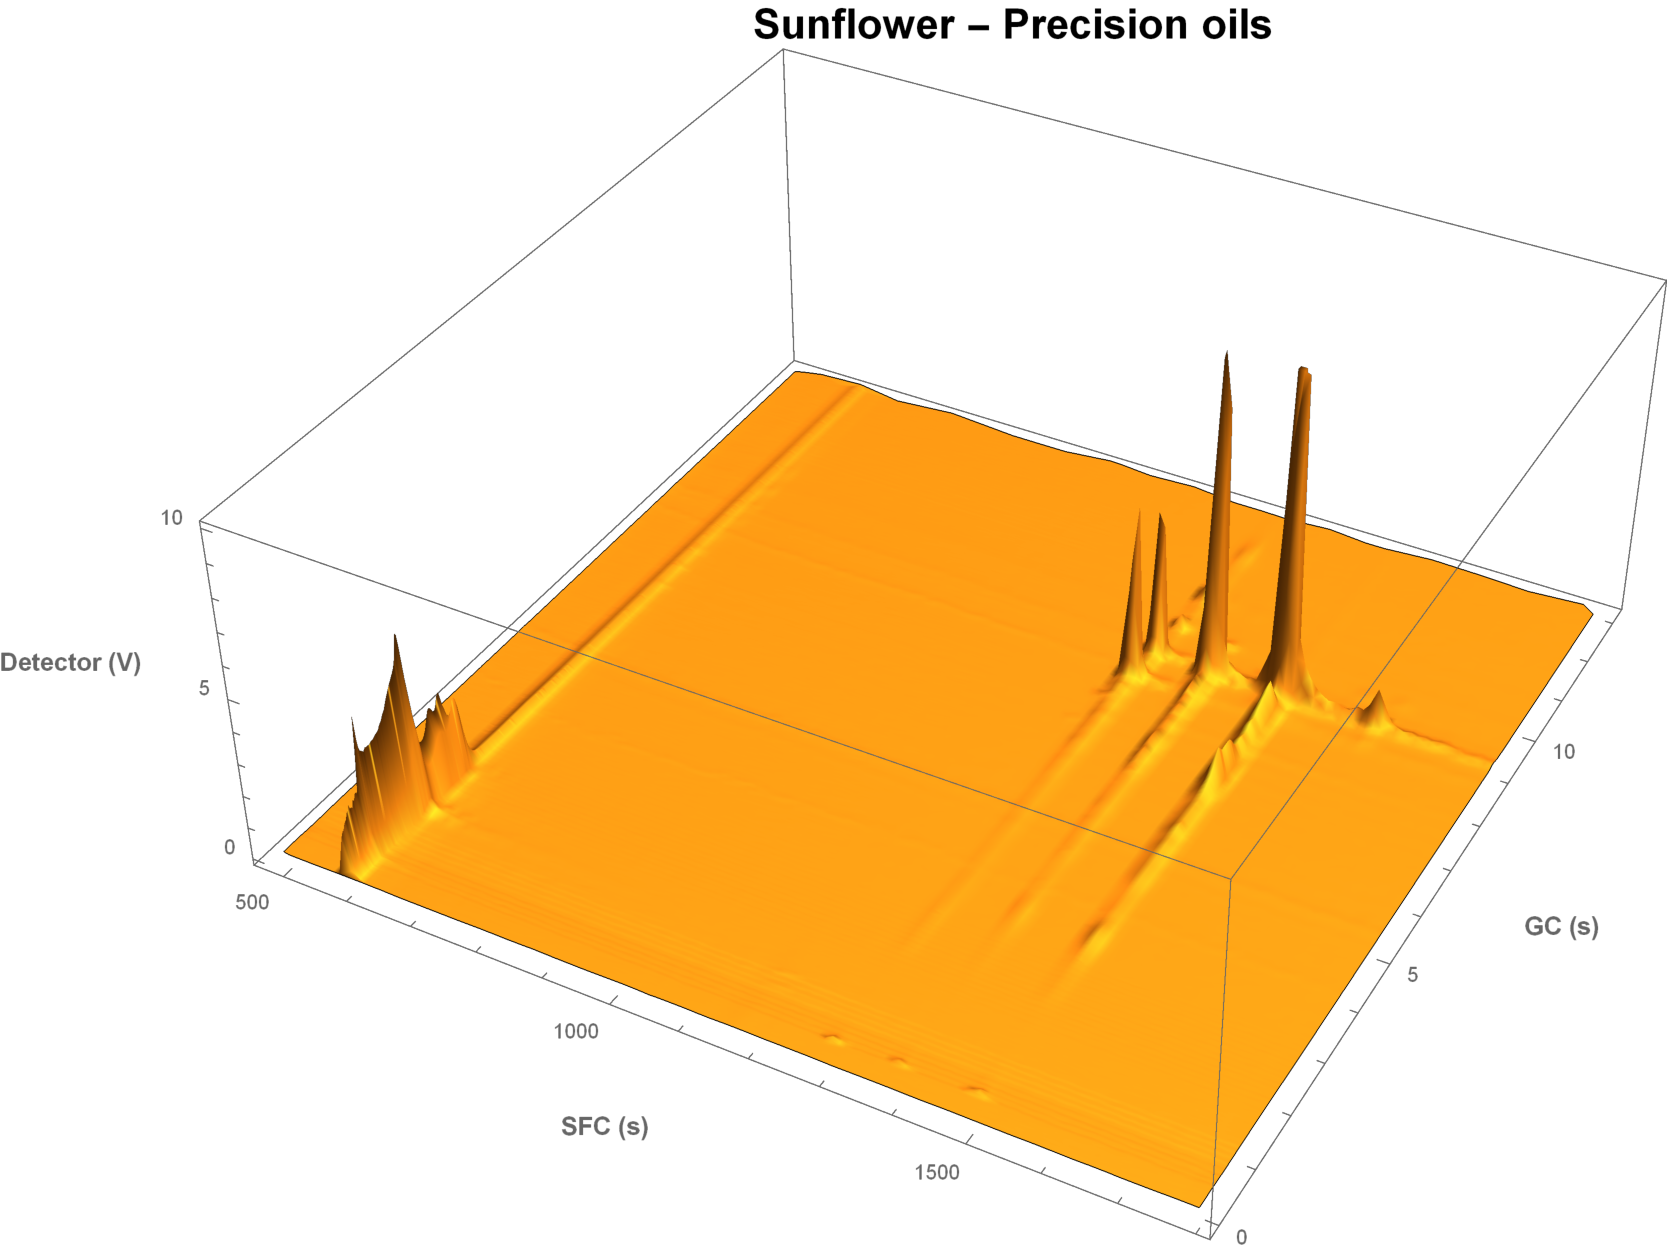
\includegraphics[width=0.8\textwidth]{Figures/2DChromatogram.pdf}
	\decoRule
	\caption[A 2D SFC×GC chromatogram]{A 2D SFC×GC chromatogram.}	
	\label{fig:2DChromatogram}
\end{figure}


\begin{figure}
	\centering
	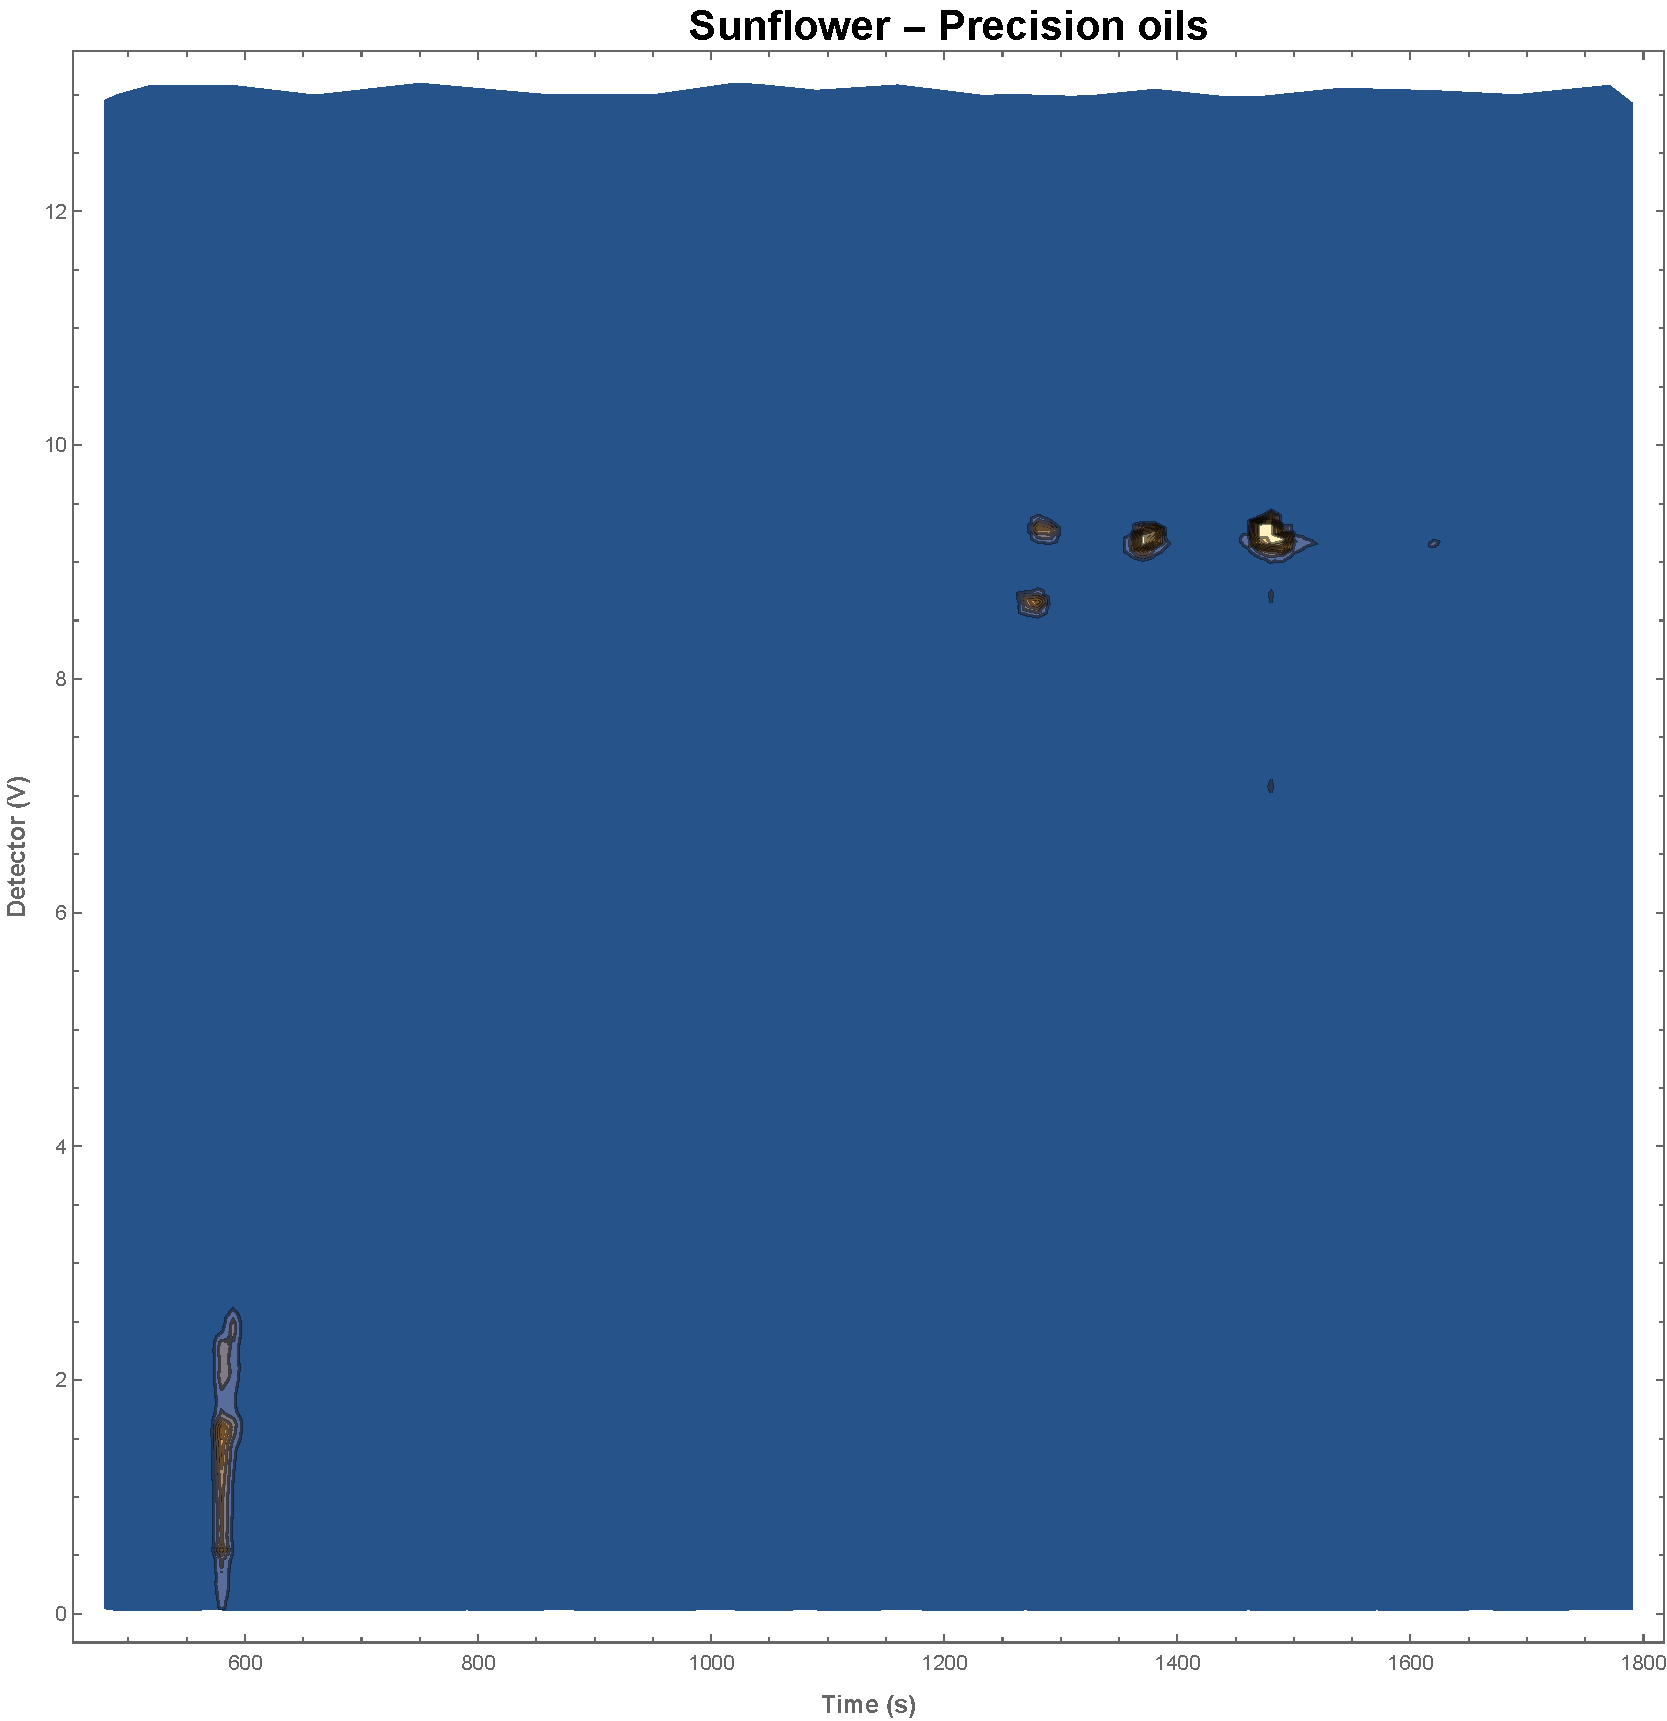
\includegraphics[width=0.8\textwidth]{Figures/Contourplot.pdf}
	\decoRule
	\caption[A 2D SFC×GC chromatogram]{An SFC×GC contour plot.}	
	\label{fig:Contourplot}
\end{figure}



 
% Chapter 6

\begin{savequote}[\quotewidth] I'm really into coconut oil for everything. I cook it,
eat it, put it in my hair, and use it as body lotion. I put it on my face, too -
day cream, night cream, whatever. I love the smell. It reminds me of the beach.
I'm not particular on what brand as long as it's organic.

\qauthor{Juliette Lewis}
\end{savequote}

\chapter{Investigating biodiesel feedstock using SFC×GC} % Main chapter title

\label{Chapter6} % For referencing this chapter elsewhere, use \ref{Chapter6}

\section{Introduction}


Biodiesel consists mostly of a mixture of methyl esters of fatty acids obtained
from plant oils. To comply with the relevant technical standard, SANS 1935,
\autocite{SANS1935} (see Chapter \ref{Chapter3}), it must consist of a mass
fraction of \SI{96.5}{\percent} or more of fatty acid methyl esters (FAME), but
not more than \SI{12}{\percent} linolenic acid methyl ester, and not more than
\SI{1}{\percent} of FAMEs with more than \num{4} double bonds.

The prescribed methods for determining the quantities of the compounds are
chromatographic, but the method for  determining the \textit{total amount} of
FAMEs is a completely different method from that for determining the amount of
\textit{unsaturated} FAMEs. Both these methods generate complex chromatograms
that need highly skilled and experienced chromatographers to interpret.

There is no doubt that the use of artificial intelligence and other
technological innovation for interpreting chromatograms will grow, but the
paradox of automation\footnote{Automation helps you least when you need it most
\autocite{Strauch2018, Bainbridge1983}.} predicts that as biodiesel production
grows, feedstocks proliferate, and complexity increase, the analytical chemist
will need better tools, methods, and instruments to understand the problems that
arise when automation fails.

Comprehensively coupled chromatography offers a way to better exploit chemistry
for improved analytical separations. It does this in three ways: the first is by
increasing the peak capacity of the system, the second is by improved
sensitivity, and the third is by generating patterns in the data.

\section{SFC of FAMEs}

The power of comprehensive chromatography is unlocked by orthogonality.
Orthogonality is the difference in separation mechanism between the two
dimensions \autocite{Marriott2012}. When FAMES are chromatographically separated
by SFC in a system using neat carbon dioxide as a mobile phase and unmodified silica as
a stationary phase, then the separation is according to the number of double
bonds, independent of chain length \autocite{Robertson1991, Smith1994,
Smith2001}. This stands in strong contrast to the separation of FAMEs by GC,
where the major separation is according to volatility, which can be adjusted,
but not overridden, by changing the polarity (or other chemical aspect) of the
stationary phase. (See Figure \ref{fig:RestekFAMEsGC}.)

\begin{figure}
\centering
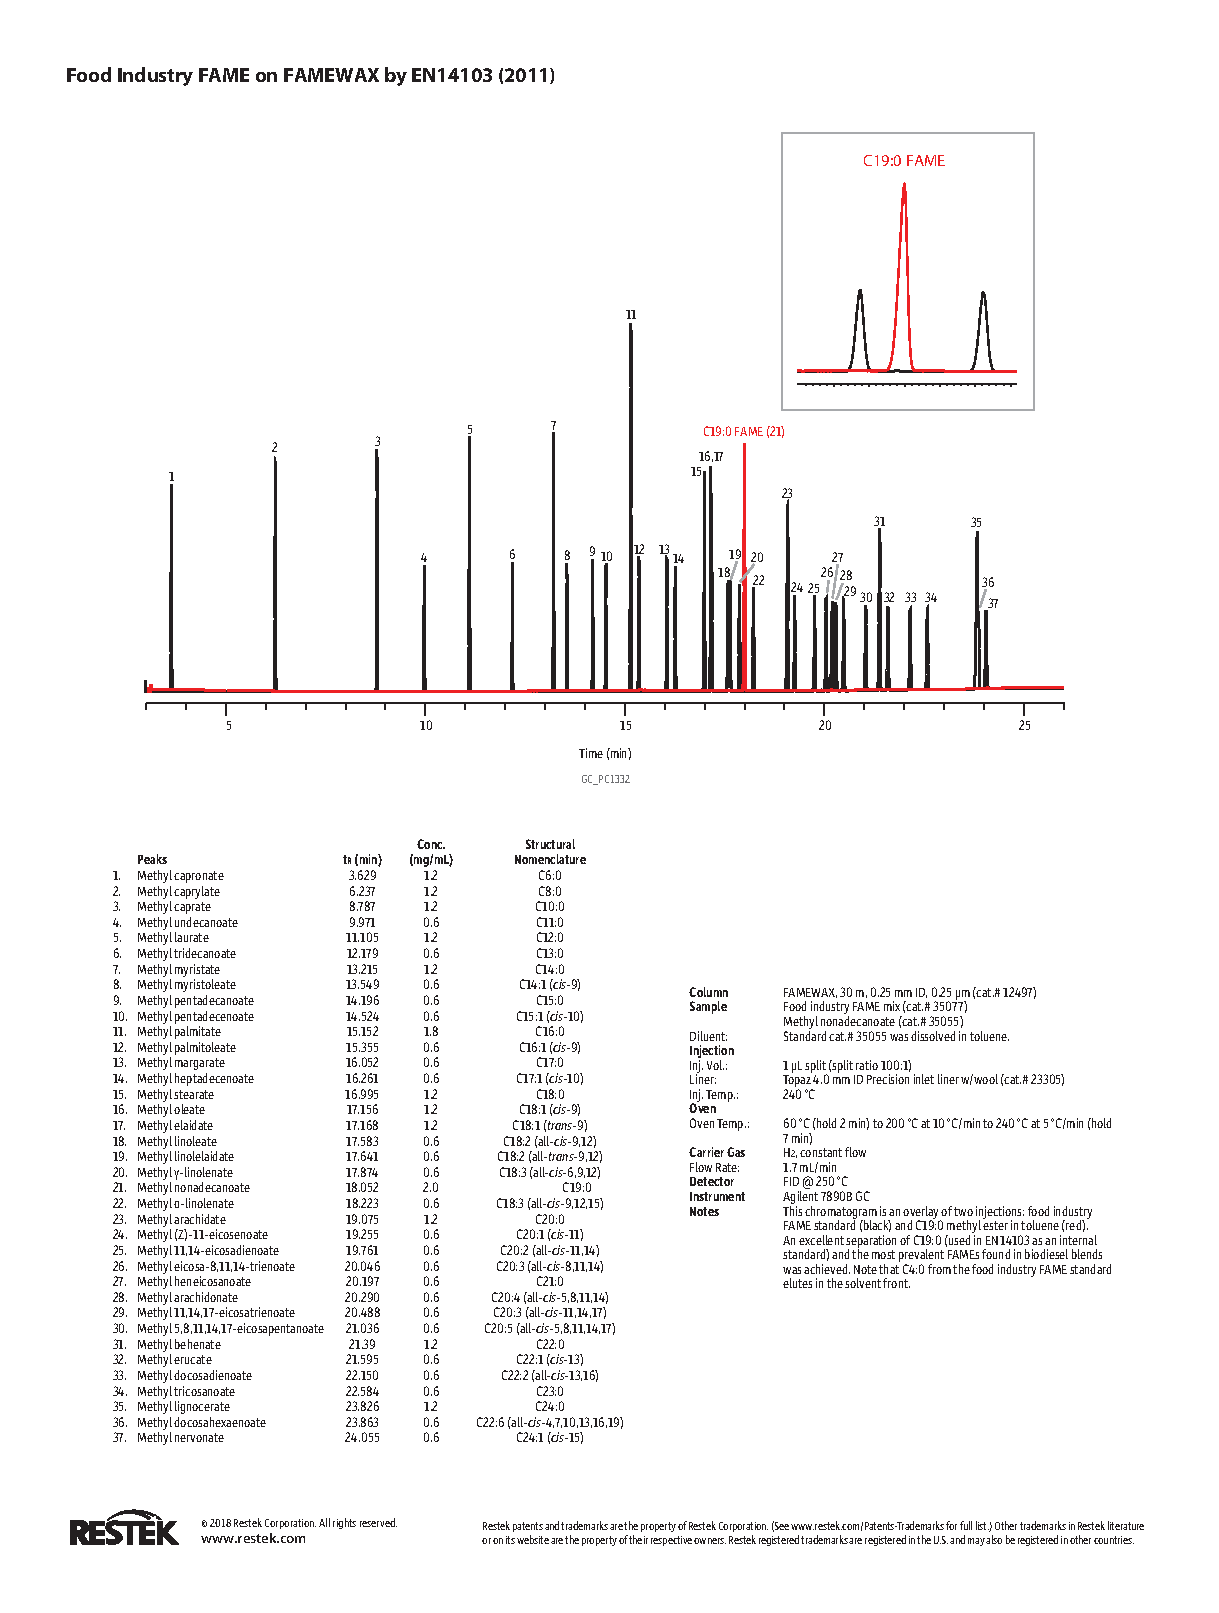
\includegraphics[width=\textwidth]{Figures/GC_PC1332.pdf}
\decoRule

\caption[Separation of FAME by GC]{This figure shows that when separating FAMEs
by GC, using specialized column, separation is primarily by fatty acid chain
length, and secondarily by number of double bonds. Reproduced with permission of Restek Corporation.}

\label{fig:RestekFAMEsGC}
\end{figure}

Silver ions are often used in stationary phases to separate unsaturated
compounds, and this includes stationary phases for SFC \autocite{Sandra2002,
Potgieter2013}. The retention mechanism is quite complex
\autocite{Nikolova-Damyanova2019}, but it offers a powerful technique for the
elucidation of lipid structures, as reviewed as early as 1966
\autocite{Morris1966}. Nevertheless, in this chapter the use of stationary
phases modified with silver ions was neither necessary nor attempted.

%As discussed in Section \ref{sec:Rancimat}, fatty acids are not stable at high
%temperatures. This means that they might degrade during chromatographic
%separation at high temperature, especially if the run times are long. Because
%SFC operates at low temperatures, the unstable compounds are less likely to
%degrade.

The utterly different retention behaviours of FAMEs on silica with a carbon
dioxide mobile phase and on GC offers high orthogonality, which promises to make
comprehensive coupling worthwhile.

\section[Coaxial heater performance.]{Performance of the coaxial heater.}

Practical SFC×GC depends on reliably repeating fast temperature programs on a
capillary gas chromatography column. The effect of these conditions on the
column will be discussed in the following sections.

\subsection{Column lifetime}

As discussed in Section \ref{sec:ChromDet}, FAMEs can be separated by gas
chromatography using a relatively non-polar columns with high-temperature
programs. For this purpose column manufacturers supply special 'high
temperature' columns, which address two aspects of column lifetime: mechanical
degradation and stationary phase degradation. The SFC×GC instrument did not use
such columns, and the following discussion explains why their use could be
avoided.

\subsubsection{Mechanical degradation}
Fused silica has a high \keyword{tensile strength}, but also a low
\keyword{fracture toughness}. This means that it is strong enough to resist the
forces involved in its use as a column, but very liable to fracture if it gets
damaged. Very small flaws, less than a micron in depth, will cause fused silica
(or any other glass) to fracture under loads far under what would be expected
from its tensile strength. Such flaws can be caused by mechanical scratches or
reaction with atmospheric water. Therefore the fused silica capillary is coated
on the outside with a layer of polyimide, which protects it from environmental
damage. The strength of the a capillary column therefore depends on the
integrity of the polyimide coating. The polyimide, like all resins and polymers,
degrade faster at higher temperatures, so the longer the column spends at high
temperature the sooner the polyimide will degrade to the point where it fails
to protect the fused silica, and the shorter the overall mechanical lifetime of
the column will be.

Traditional advice to chromatographers is to use temperature programs that
minimize the time spent at high temperature, which will contribute to longer
column lifetimes. The usual way to do it is to to use a temperature program with
a maximum temperature no higher than necessary, but the same cumulative time at
high temperature can be obtained by using higher temperatures but for shorter
periods. Fast temperature programs expose the columns for only very brief
periods at high temperature.

(Column mechanical lifetime can also be improved by using metal capillaries.
Metals are not afflicted by brittle fracture the way fused silica is, but they
don't offer the chemical inertness of fused silica. To exploit the fracture
toughness of metal technologies have been developed to deactivate metal surfaces
\autocite{Smith2002}, which makes metal columns a modern possibility. Column
manufacturers offer metal columns specifically designed for biodiesel analysis.)

Another durability benefit of the stainless steel coaxial heater is that the
outer surface of the capillary column is protected from mechanical damage by
encasement in the stainless steel tube of the coaxial heater. During development
of the coaxial heater there were occasions where the column was accidentally
overheated by poorly-controlled resistive heating. Even though the polyimide
coating had been completely charred away and the capillary was fragile, the
column was intact and still provided separations.

Using carbon dioxide as a between-program coolant also protects the polyimide
coating from oxidative damage by purging the column environment of oxygen.

\subsubsection{Stationary phase degradation}

The stationary phases inside the GC columns face degradation similar to the that
of the polyimide. Column manufacturers minimize sta\-tion\-ary phase degradation
by using improved technologies like cross-linked resins, or polymers with
backbones resistant to certain degradation mechanisms \autocite{Day2003}.
Using fast temperature programs help extend stationary phase lifetime by
minimizing the cumulative time the column spends at high temperature.

\subsubsection{Column bleed}
Short columns and fast temperature programs have another beneficial side effect:
reduced \keyword{column bleed}. Any resin- or polymer-based stationary phase
degrades over time, and this degradation is faster at higher temperatures
\autocite[p. 66]{Mcnair2019}. It is observed as a rise in baseline during the
high temperature part of a temperature program. Various stationary phase
technologies can be employed to reduce column bleed, but because the amount of
column bleed depends on the amount of stationary phase it is clear that a
\SI{1}{\metre} column will have \num{1/30}th of the column bleed of a
\SI{30}{\metre} column with the same stationary phase. Despite using temperature
programs that went up to the temperature limit recommended by the column
manufacturer, column bleed was not a significant feature in the obtained
chromatograms.

\subsection{Thermal shock}
An aspect of fast temperature programming with such a temperature range as used
in this study (\SIrange{-30}{400}{\celsius}) is \keyword{thermal shock}. Thermal
shock occurs when an object is subjected to a rapid change in temperature. Under
such non-equilibrium conditions different parts of the object will have
different temperatures. The material that the object is made of has a certain
\keyword{coefficient of thermal expansion}, which means that the relative sizes
of the parts of the object at different temperatures will differ. This will
cause stress between the parts, and if the stress exceeds the strength of the
material, the material will fracture. Fused silica has a low coefficient of
expansion (\SI{0.55e-6}{\per\kelvin}, compared to the \SI{9.0e-6}{\per\kelvin}
of soda lime glass or the \SI{4.0e-6}{\per\kelvin} of borosilicate glass) and
therefore experiences low thermal shock. The amount of material in a capillary
is also relatively small, which keeps temperature gradients small and therefore
stresses low. We didn't observe any column failures that could be ascribed to 
thermal shock.

\subsection{Thermal fatigue}

Another cause of material failure due to temperature is \keyword{thermal
fatigue}. ``Thermal fatigue (TF) is the gradual deterioration and eventual
cracking of a material by alternate heating and cooling during which free
thermal expansion is partially or completely constrained'' \autocite{Rao2001}.
The expansion of the portion of the fused silica column subjected to alternate
heating and cooling is not constrained, and the part of the fused silica column
that is constrained (in the sealing ferrules) is not subjected to alternate
heating and cooling (it is held at constant temperature in the heated T-piece
block) therefore we do not expect thermal fatigue. We did not explicitly test
for the occurrence of thermal fatigue, but we did not encounter column failure
that could be attributed to thermal fatigue.

\subsection{Corrosion}
One failure of the coaxial heater could be attributed to corrosion. The joint
between the coaxial heater and the heated T-piece block is brazed, and there was
a failure of the thin-walled stainless steel tube near that joint, in the
portion heated during the brazing operation. Visual inspection seemed to
indicate thinning caused by corrosion. An acid flux was used during the brazing,
which might have contributed to the corrosion, especially in the presence of
water condensed from the atmosphere during the cooling of the column.

\subsection{GC retention time precision}

During the development of the resistive heater it was shown that the measured
temperature ramps are highly repeatable. But the retention times of of compounds
being separated by GC are highly sensitive to temperature, so it was necessary
to obtain a measure of the retention time repeatability.

To estimate the retention time variance, two alkanes (dodecane and hexadecane)
were added to the SFC mobile phase at low concentration. These compounds are not
retained on the silica at all, and are therefore present in all the GC runs at
the same concentration and all the peaks should be identical. Variance in peak
retention, -area, and -height therefore indicate the repeatability of the fast
GC system. Variability of retention time is summarized in Table
\ref{tab:RetentionTimeVariance}

\begin{table}

	\caption{\label{tab:RetentionTimeVariance}A summary of retention time repeataility of alkanes
separated on the fast temperature programmed chromatograph.}
	\centering
	\begin{tabular}{lllll}
	\toprule
	\tabhead{Compound} & \tabhead{n} & \tabhead{t\textsubscript{r} (s)} & \tabhead{S.D. of t\textsubscript{r} (s)}	& \tabhead{R.S.D. of t\textsubscript{r} (\%)} \\
	\midrule
	Dodecane 			& 73 		& 5.07 								& 0.023 									& 0.46\\
	Hexadecane			& 73 		& 6.58 								& 0.052 									& 0.78\\
	\bottomrule
\end{tabular}

\end{table}

The peak widths were about \SI{500}{\milli\second}, so the
\SI{20}{\milli\second} standard deviation for hexadecane means that the
variation in retention time is only about \SI{10}{\percent} of the peak width.
The relative standard deviations (RSD) of retention times were similar to those
obtained in GC×GC \autocite{Shellie2002}.

\section[Study of biodiesel by SFC×GC]{Study of potential biodiesel feedstock by SFC×GC}

Biodiesel can be produced from any combination of a variety of vegetable oils.
Indeed, to ensure conformance to standards it might be necessary to produce
biodiesel from blends or combinations of oils. But as an introduction it is
instructive to start by analysing the FAMEs obtained from unblended oils.

\subsection{Samples}

Various samples of edible vegetable oil were obtained from
supermarkets. (See Table \ref{tab:OilSamples})

\begin{table}
	\caption{Oils used for FAME analysis}
	\label{tab:OilSamples}
	\centering
	\begin{tabular}{l l l}
	\toprule
	\tabhead{Oil} & \tabhead{Brand} & \tabhead{Species} 			\\
	\midrule
	Canola			& Spar			& \textit{Brassica napus}		\\
	Sunflower oil	& Pick n Pay 	& \textit{Helianthus annuus}	\\
	Coconut oil  	& Lemcke 		& \textit{Cocos nucifera}		\\
	Flax seed oil 	& Lemcke 		& \textit{Linum usitatissimum}	\\
%	Olive oil 		& Hojiblanca	& \textit{Olea europaea}		\\
	\bottomrule\\
	\end{tabular}
\end{table}

\subsection{Sample preparation}

Fatty acids in oils might be either free or bound to glycerol. To quantitatively
convert them to FAME therefore requires that the bound fatty acid be transesterified,
and the free fatty acids esterified. Both transesterification and esterification
can be achieved by acid catalyst, but this reaction is quite slow. Basic
catalysts can rapidly transesterify acyl glycerols, but will not esterify free
fatty acids.

The method used involved first treating the oil sample with sodium hydroxide
dissolved in dry methanol. The methanol acts as a solvent but also provides an
excess of methanol so that the transesterification reaction is driven to
completion. On completion of the reaction an excess of acid is added, which
neutralizes the base and esterifies any free fatty acids. Then an organic
solvent and water are added, which provides two phases: the non-polar FAMEs
dissolve in the organic layer, and the polar glycerol and salts dissolve in the
water layer.

\subsubsection{Method}

This method is based on an official method \autocite{AOCS2017}, modified in two
respects. First, the acidic catalyst boron trifluoride is replace by sulphuric
acid, and second, hexane is used instead of heptane.

\begin{enumerate}
  
\item Transfer \num{4} drops of melted sample to a \SI{20}{\milli\litre} glass
stoppered test tube. Add a few boiling stones

\item Add \SI{2}{\milli\litre} NaOH/Methanol solution (0.5N) and boil for
\SI{11}{\min} under reflux.

\item Add \SI{2}{\milli\litre} H\textsubscript{2}SO\textsubscript{4}/Methanol
solution via condenser and boil for \SI{2}{\minute}

\item  Add \SI{2}{\milli\litre} hexane via the condenser and boil for
\SI{1}{\minute}.

\item Remove the test tube from the heat source and leave to cool.

\item Add \SI{4}{\milli\litre} saturated NaCl and mix gently.

\item Allow the phases to separate. Transfer the hexane layer to a vial and use for injection.

\end{enumerate}

\subsection{SFC}

A \SI{0.5}{\micro\litre} volume of the hexane layer was injected into the neat
carbon dioxide mobile phase, as described in Section \ref{sec:SFCInjection}. The
column was five HPLC columns (150 mm $\times$ 4.6 mm, 3 $\mu$m particles)
(Restek, Pinnacle DB Silica) connected in series.

\subsection{Modulation}

The modulation period was \SI{10}{\second} during which the fractions of the SFC
eluate were transferred to the GC inlet via a linear restrictor. In the hot
(\SI{350}{\celsius}) inlet the fractions were evaporated and were swept onto the
cold (\SI{-20}{\celsius} column they were trapped in the stationary phase.
\SI{3}{\second} after the collection period ended the vent valve opened for
\SI{1}{\second} to vent excess pressure from the GC inlet.

\subsection{GC}

The fast temperature program ramped the GC column temperature from
\SI{-20}{\celsius} to \SI{350}{\celsius} in \SI{10}{s}
(\SI{2200}{\celsius\per\second}), maintaining \SI{350}{\celsius} for
\SI{2}{\second}. Then the cooling system would activate and cool the column to
\SI{-20}{\celsius} or below, ready to trap the next SFC fraction. The FID
detector was kept at \SI{350}{\celsius}.

In this way a series of GC chromatograms of SFC fractions were recorded, which
were assembled into a 2D chromatogram. Figure \ref{fig:2DCanola} shows
a 2D chromatogram of a sample of FAME prepared from canola oil. This 2D
chromatogram consists of 132 fast GC chromatograms collected in approximately 90
minutes.

\subsection{Results and discussion}

\begin{figure}
\centering
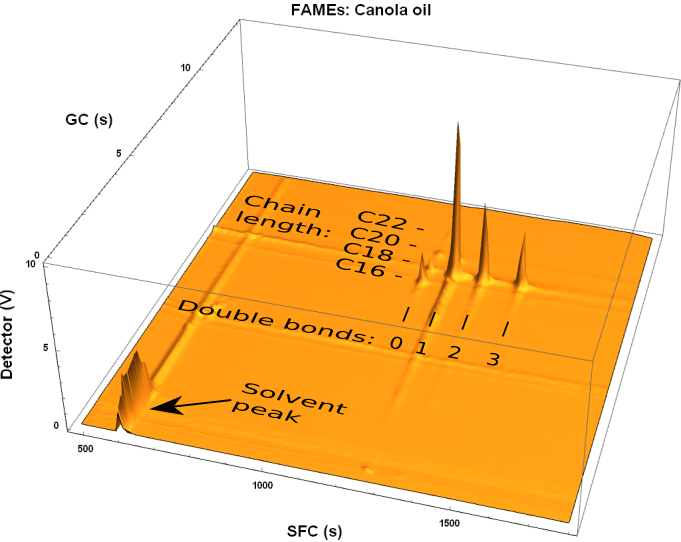
\includegraphics[width=\textwidth]{Figures/Interpretation.png}
\decoRule

\caption[SFC×GC of canola oil]{A 2D chromatogram of FAMEs derived from
canola oil. It is clear that the oil consists mostly of unsaturated fatty
acids.}

\label{fig:2DCanola}
\end{figure}

The chromatogram shown in Figure \ref{fig:2DCanola} is very simple to interpret.
In the SFC dimension, separation is by number of double bonds.
This means that FAMEs without double bonds elute first in this dimension,
followed by FAMEs with one, two and three double bonds respectively. There is
good resolution between the peaks in the SFC dimension.

The volatility of a FAME depends primarily on the length of the carbon atom
chain, therefore the separation in the GC dimension is by chain length. Because
these FAMEs are of biological origin, we expect their chains to have an even
number of carbon atoms. From the literature we know that oleic acid (C18:1) is
the most common fatty acid in canola oil \autocite{JFAOWHOCAC2019}, and that
therefore the major peak in the chromatogram is a C18 FAME. This allows us to
easily identify the peaks for C16, C18, C20 and C22 in the GC dimension.

By inspecting this chromatogram we can confirm that canola oil is a vi\-able
biodiesel feedstock: The unsaturated compounds have mostly a single double bond,
which should make it oxidatively stable, and the quantities of unsaturated FAMEs
are low, which means that it will most likely have suitable cold-flow
properties, because unsaturated FAMEs have higher freezing points than saturated
FAMEs.

\begin{figure}
\centering
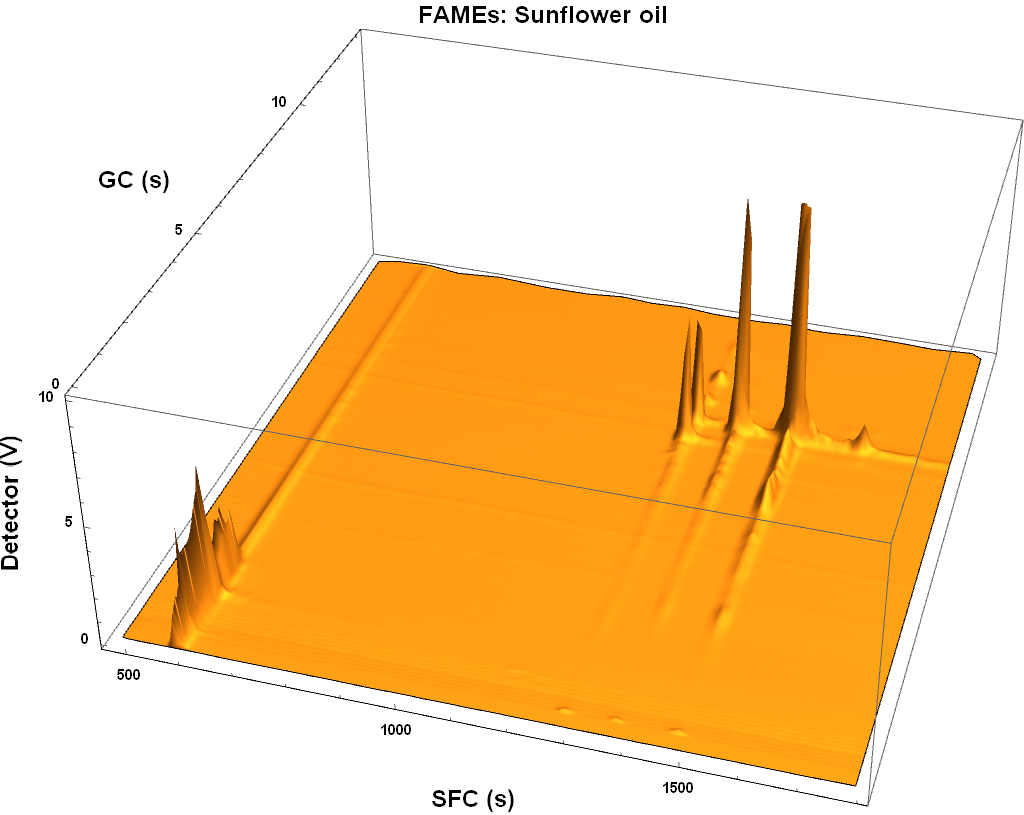
\includegraphics[width=\textwidth]{Figures/Sunflower.png}
\decoRule

\caption[SFC×GC of sunflower oil]{A 2D chromatogram of FAMEs derived from
sunflower oil. It is clear that the oil consists mostly of unsaturated fatty
acids, with a high proportion of linoleic acid (C18:2)}

\label{fig:2DSunflower}
\end{figure}

\subsection{Sunflower oil}

Figure \ref{fig:2DSunflower} shows an SFC×GC chromatogram of FAMEs obtained from
sunflower oil. The biggest peak in the chromatogram corresponds to linoleic acid
methyl ester (C18:2). This agrees with the literature, which indicates that the
main, traditional cultivar of sunflower produced in South Africa is of the
high-linoleic type, with a fatty acid profile of \SI{69}{\percent} linoleic
acid, \SI{20}{\percent} oleic acid, and \SI{11}{percent} saturated fats
\autocite {JFAOWHOCAC2019}.

This sunflower oil chromatogram was compared to a fatty acid profile obtained by
a professional oil analysis laboratory\footnote{Precision Oil Laboratories,
info@precisionoils.co.za,  +27 15 307 7208, SANAS Testing Laboratory T0802}.
(See Table \ref{tab:SunflowerPrecisionOils}.) The fatty acid profile data was
plotted on a 3D bar chart (See Figure \ref{fig:2DSunflowerBarChart}). The axes
of the bar chart were chosen to plot the fatty acid profile information in a
similar space and scale as the chromatogram (Figure \ref{fig:2DSunflower}). It
can be seen that the bar chart shows the same information as the chromatogram.
The information in the bar chart has been obtained from a 1D chromatogram by
integrating peaks, calculating amounts of FAMEs from peak areas, and then
plotting those amounts in the bar chart, whereas the SFC×GC chromatogram is a
plot of FID response and involves no quantification.

This chromatogram suggests that sunflower oil will make a suitable feedstock for
biodiesel: the relatively high amount of unsaturated FAs would seem to imply
suitable cold flow properties. The relatively high degree of unsaturation does
suggest caution regarding oxidative stability.

\begin{figure}
\centering
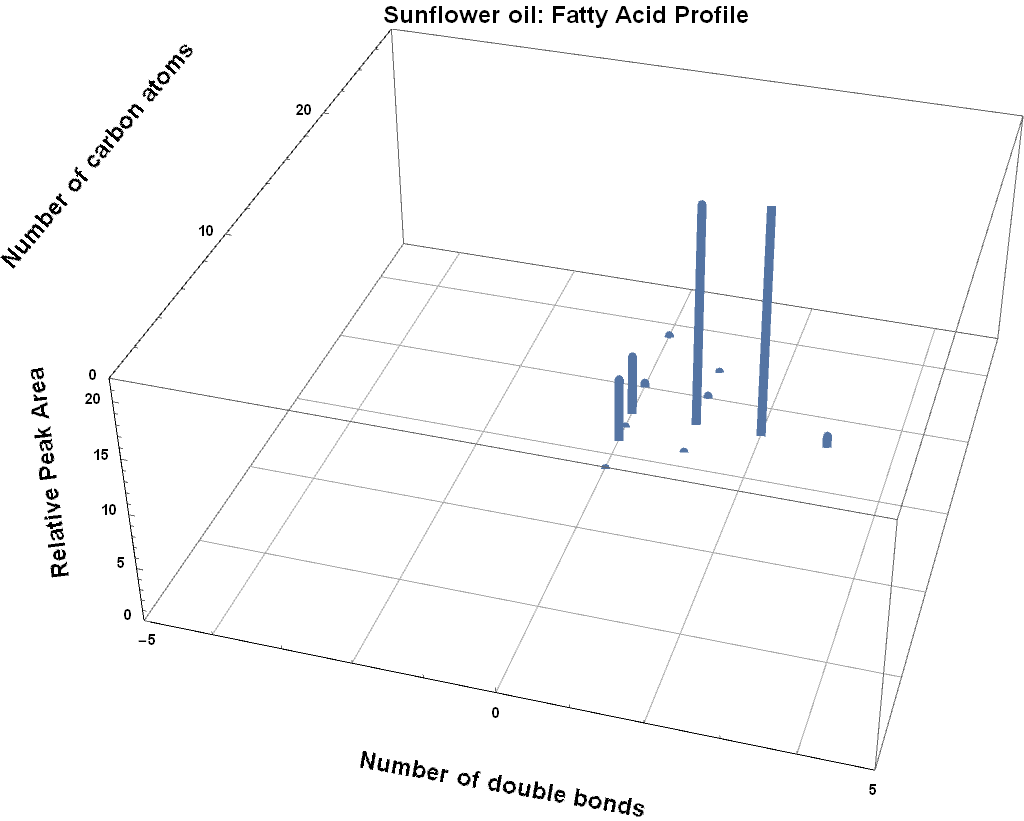
\includegraphics[width=\textwidth]{Figures/BarChart.png}
\decoRule

\caption[3D Bar chart of fatty acid profile]{The fatty acid profile of a
sunflower oil, when plotted on a suitably-scaled bar chart, shows how well the
SFC×GC chromatogram of the same oil (Figure \ref{fig:2DSunflower}) represents
the same data without any processing.}

\label{fig:2DSunflowerBarChart}
\end{figure}

\subsection{Coconut oil}

Figure \ref{fig:2DCoconut} shows the SFC×GC chromatogram of FAMES from coconut
oil (\textit{Cocos nucifera L}). It is clear that the dominant FAMEs in coconut
oil are saturated.

The high saturation of coconut oil makes it oxidatively stable, but the high
melting point of the saturated FAMEs also means that it might not meet
cold flow requirements.

The high oxidative stability of coconut oil makes it resistant to going rancid,
which means it has been used since antiquity as a natural ingredient for cosmetics
\autocite{Berdick1972}.

\begin{figure}
\centering
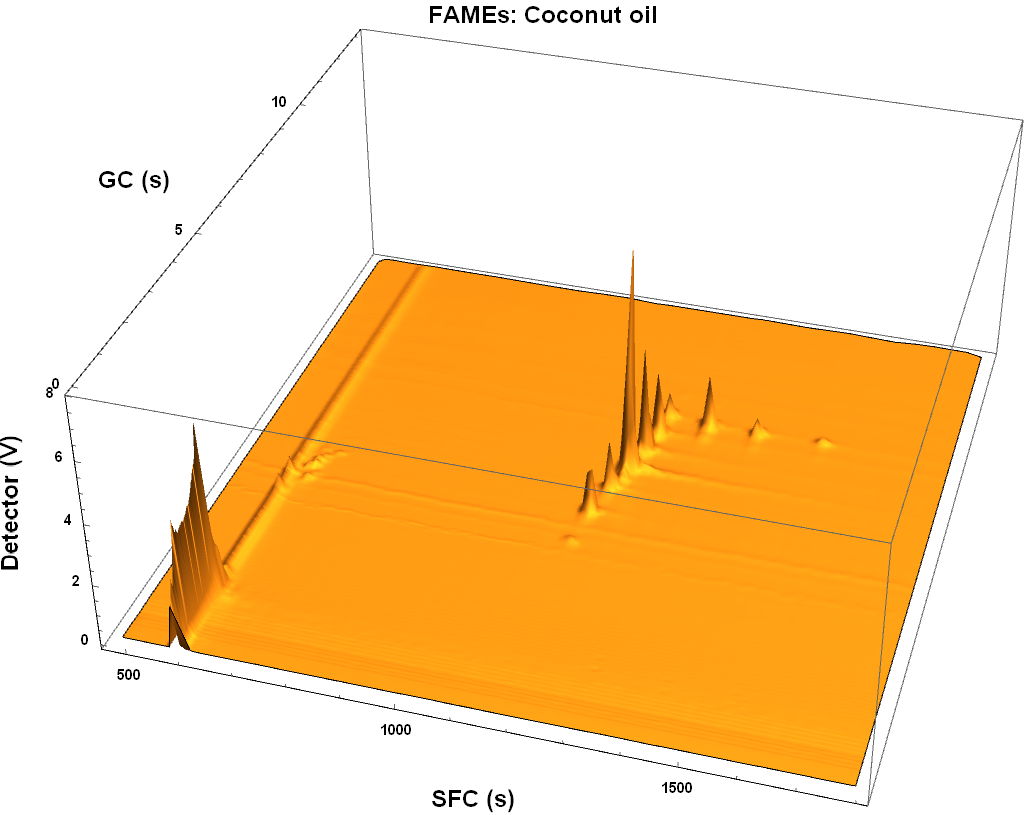
\includegraphics[width=\textwidth]{Figures/Coconut.png}
\decoRule

\caption[SFC×GC of coconut oil]{A 2D chromatogram of FAMEs derived from
coconut oil. It is clear that the oil consists mostly of saturated fatty
acids.}

\label{fig:2DCoconut}
\end{figure}

\subsection{Flax seed oil}

Figure \ref{fig:2DFlax} shows an SFC×GC chromatogram of FAMEs obtained from flax
seed oil. This oil is obtained from the seeds of the annual plant \textit{Linum
usitatissimum}, and was sold as an edible oil.

\begin{figure}
\centering
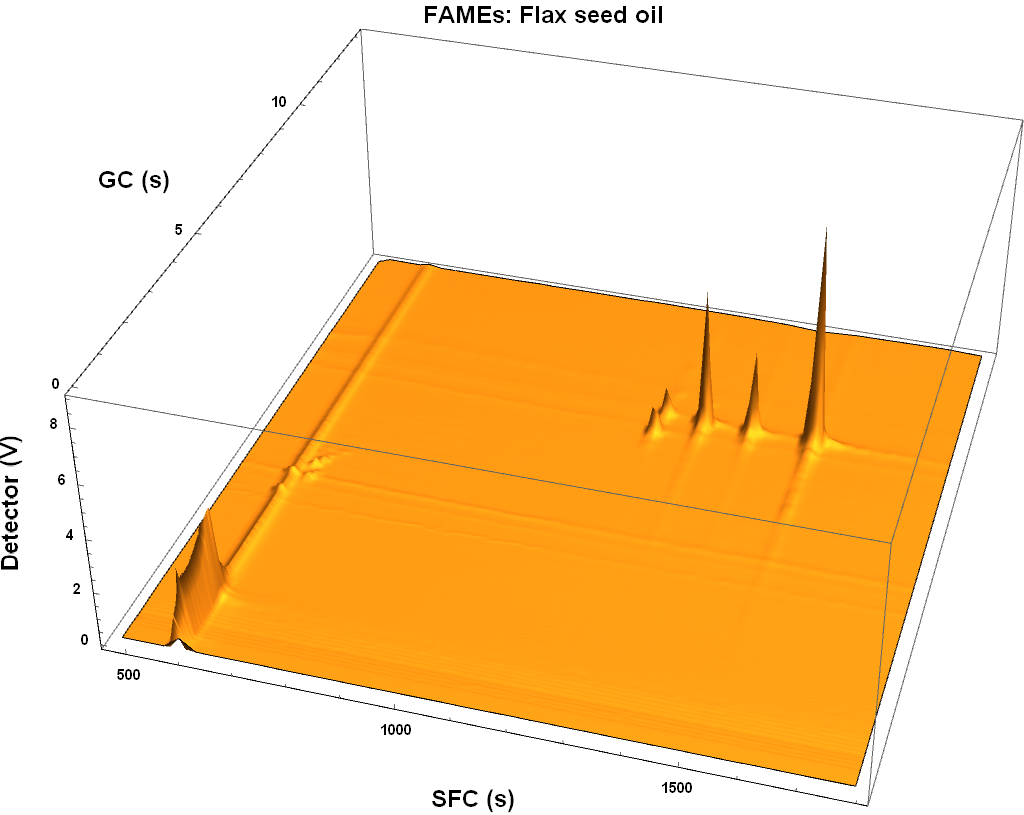
\includegraphics[width=\textwidth]{Figures/Flax44.png}
\decoRule

\caption[SFC×GC of flax seed oil]{A 2D chromatogram of FAMEs derived from
flax seed oil. It is clear that the oil consists mostly of highly unsaturated fatty
acids.}

\label{fig:2DFlax}
\end{figure}

The chromatogram shows that the major fatty acid component of this oil is
linolenic acid (C18:3). This will immediately inform a producer that flax seed
oil would not be a suitable feedstock for biodiesel: SANS 1935 limits the
linolenic acid fraction to less than \SI{12}{\percent} (See section
\ref{sec:ChromDetUnsat}).

Flax seed oil only recently became considered a food or a food supplement: the
1911 edition of the Encyclopaedia Britannica only mentions it as a food by
saying ``The oil is to some extent used as food in Russia and in parts of Poland
and Hungary" \autocite{Linseed1911}, and remarks that the oil is edible when it
is cold pressed. This is not surprising, because the oil goes rancid very
quickly, leaving it unpalatable.

Historically the more common name for the oil has been \keyword{linseed oil} and
it was mostly used for industrial purposes, particularly paint and varnish.
As the encyclopedia puts it: ``Commercial linseed oil has a peculiar, rather
disagreeable sharp taste and smell.'' The oil of used in artists' oil paints is
most commonly refined and prepared linseed oil. This oil is classed as a
\keyword{drying oil}, because a layer of this oil exposed to air becomes solid,
or ``dry". This is the result of the high degree of unsaturation of the oil,
which rapidly causes oxygen-mediated polymerization. Exposure to air over time
makes the oil become more viscous and eventually solid, making it a suitable
base for paint, particularly if the oil has been pre-treated. In biodiesel such
polymerization could cause clogging or the formation of objectionable sludge.


\section{Biodiesel blends}

\subsection{Introduction}
Biodiesel can be blended in all proportions with diesel obtained from petroleum
(petrodiesel). The volatility of biodiesel is slightly lower than that of
petrodiesel, but in 1D gas chromatography the biodiesel compounds with higher
volatility overlap significantly with the petrodiesel compounds of lower
volatility. One example of an attempt to overcome this problem is the use of a
highly polar ionic liquid column, which increases the retention of the FAMEs in
the blend relative to the retention of the petrodiesel hydrocarbons
\autocite{Ragonese2009}.

On a polar stationary phase like bare silica with a non-polar stationary phase
like carbon dioxide, the hydrocarbons from petrodiesel are not expected to be
significantly retained. But, as shown in the in the previous section, under such
conditions FAMEs are retained and separated. When we inject a blend of biodiesel
and petrodiesel on SFC×GC, we therefore expect the biodiesel portion to be
completely separated from the petrodiesel portion.

\subsection{Sample}

A B50 biodiesel blend was prepared by mixing equal volumes of biodiesel and
petrodiesel in the laboratory. The biodiesel sample was donated by a commercial
testing laboratory and had been produced from waste cooking oil by an anonymous
producer. The petrodiesel sample (Shell Extra Diesel 500 ppm) was obtained from
a consumer filling station.

The injection system described in Section \ref{sec:SFCInjection} was used to
inject a \SI{0.5}{\micro\litre} volume of this undiluted B50 blend.

\subsection{SFC}

The SFC used neat carbon dioxide at \SI{200}{\bar} inlet pressure as mobile
phase. The column consisted of five HPLC bare silica columns (150 mm $\times$
4.6 mm, 3 $\mu$m particles) (Restek, Pinnacle DB Silica) connected in series.

\subsection{Modulation}

The SFC eluate fractions \SI{2}{\second} were collected on the GC column
cooled to a temperature of \SI{-20}{\celsius}. Tto he inlet vent was held closed
for \SI{4}{\second}, and then opened for \SI{1}{\second} to release excess
pressure.

\subsection{GC}

The column used in the fast gas chromatograph was an OV-5 column, which has a
stationary phase comprised of \SI{5}{\percent} diphenyl, \SI{95}{\percent}
dimethylpolysiloxane. It was \SI{1}{\metre} long, with an internal diameter of
\SI{0.25}{\milli\metre}. The thickness of the stationary phase was
\SI{0.25}{\micro\metre}.

The temperature was ramped from \SI{-20}{\celsius} at a rate of of
\SI{1800}{\celsius\per\minute} to \SI{250}{\celsius}, where it was maintained
for \SI{6}{s}. After the temperature program had ended the column was cooled to
\SI{-20}{\celsius} again and the next fraction was collected.

The detector was an FID at \SI{250}{\celsius}. The FID response was recorded,
and so a total of 371 fast GC chromatograms were collected to compile the 2D
chromatogram.

\subsection{Results and discussion}
\label{sec:B50Discuss}
\begin{figure}
	\centering
	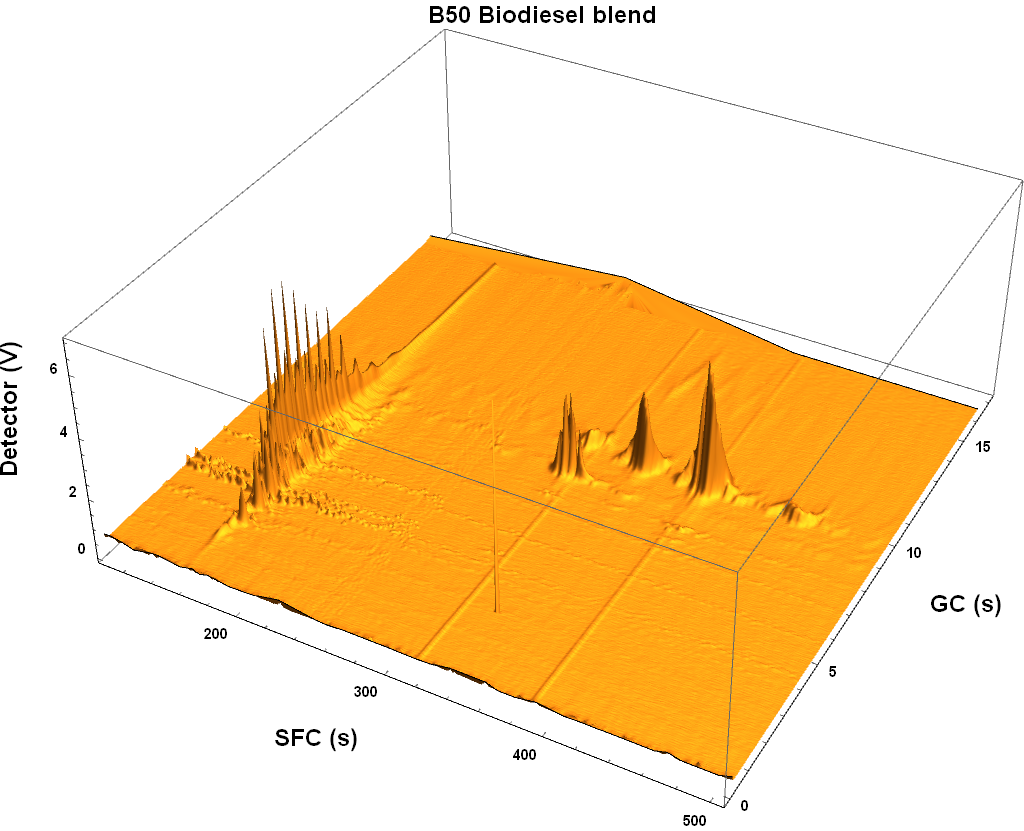
\includegraphics[width=\textwidth]{Figures/B50.png}
	\decoRule	
	
\caption[Biodiesel separated from petrodiesel.]{The separation of the biodiesel
fraction and the petroleum fraction of a biodiesel blend. SFC: Neat
CO\textsubscript{2} at 200 bar on Restek Pinnacle DB Silica column, 5 × \SI{150}{\milli\metre} ×
\SI{4.6}{\milli\metre}, \SI{3}{\micro\metre} particles. GC: Hydrogen carrier on
OV-5 \SI{1}{\metre} × \SI{0.25}{\milli\metre} × \SI{0.25}{\micro\metre},
temperature program \SI{-20}{\celsius} to \SI{250}{\celsius} at
\SI{1800}{\celsius\per\minute} hold for \SI{6}{\second}. GC runs: 371.}

	
	\label{fig:B50} 
\end{figure}

The chromatogram of the biodiesel/petrodiesel blend (Figure \ref{fig:B50}) shows
that the blend has been separated into two distinct groups of compounds. At a
retention time in the \textsuperscript{1}D (SFC) dimension of about
\SI{160}{\second} the hydrocarbons from the petrodiesel part of the blend
elutes. To those familiar with petrochemical chromatography the characteristic
unresolved complex mixture (``hydrocarbon hump'') topped by alkane peaks will be
instantly recognizable as a representing a petroleum product. (See Figure
\ref{fig:HCHump} for an example.)


\begin{figure}
	\centering
	\includegraphics[width=\textwidth]{Figures/hchump.pdf}
	\decoRule	
	
\caption[An example of a petrochemical fuel chromatogram.]{An example of a GC
chromatogram obtained from a petroleum-based diesel fuel sample, showing the
unresolved complex mixture topped by alkane peaks.}
	
	\label{fig:HCHump} 
\end{figure}

Between the \textsuperscript{1}D retention times of \SI{300}{\second} and
\SI{480}{\second} the peaks of the FAMEs are seen, clearly separated by number
of double bonds in the SFC dimension, and by volatility in the GC dimension.
When compared to Figure \ref{fig:2DSunflower}, one can surmise that the
feedstock for the biodiesel was waste sunflower oil.

As an aside, it is worth pointing out that the hydrocarbons from the petrodiesel
fraction of the blend were also separated on the SFC dimension. This is not
surprising: the standard ASTM D 5186 provides a method for the determination of
aromatic compounds in diesel by SFC \autocite{ASTMD5186}. The method separates
the unretained non-aromatics from the monoaromatics and from the polynuclear
aromatics. The SFC×GC method provides additional information about the
volatility of those aromatics which could help to quantify or identify them, but
that falls outside the scope of this discussion.

This separation shows that SFC×GC can be used to investigate the biodiesel
component of petrodiesel/biodiesel blends without sample pretreatment or
specialized columns.

Being able to determine the biodiesel content of biodiesel blends may prove
useful in at least two scenarios: 

The first is in monitoring blending. Biodiesel, essentially a mixture of esters,
is quite polar compared to petrodiesel, essentially a mixture of hydrocarbons.
This means that blending might not be a matter of just pumping the relevant volumes
of the respective fuels into a tank and relying on diffusion to complete the
mixing. Being able to determine the amount of biodiesel in different samples of
a blend will provide assurance that the blend is homogenous and should perform
according to expectations. While such a test is perhaps better performed using a
spectroscopic method, SFC×GC can provide information for calibration, and will
of course be invaluable during trouble shooting.

The second application of SFC×GC is in regulating biodiesel content. In some
political environments fuels might be taxed according to their
biologically-derived content, for example to promote agriculture or to meet
carbon emissions targets. Sometimes biological content is not encouraged by
taxation, but simply mandated. Such incentives and mandates are of course liable
to corruption, and therefore the ability to monitor the blending of the fuels is
needed. The most reliable way to differentiate between organic matter derived
from biological sources and organic matter derived from fossil sources is a
radiochemical method, where the content of radioactive \textsuperscript{14}C is
determined. (Organic material from fossil sources contains no
\textsuperscript{14}C.) The technical standard ASTM D6866 provides an approved
method. But this requires specialized equipment and trained staff, whereas fuel
laboratories more often have experience with chromatographic techniques and
might find SFC×GC a useful technique to provide evidence that a diesel fuel
blend contains the stated amount of biodiesel.

\section{Conclusion}

Comprehensively coupled chromatography offers better analytical separations in
three ways: improved peak capacity, improved sensitivity, and more structured
data. The examples presented here does not pretend to prove improved peak
capacity: biodiesel is not normally considered a chromatographically-challenging
complex sample. Neither is improved sensitivity relevant: determining biodiesel
components is not a trace analysis problem for which high sensitivity is
necessary. What these examples do show is that the high orthogonality between
SFC and GC provides data that contains a clear and powerful pattern that greatly
simplifies interpretation.

In the example of FAMEs derived from various vegetable oils the pattern shows
how the degree of unsaturation provides separation on the first dimension, and
the volatility provides separation on the second dimension. These separations,
combined in one 2D chromatogram, provides intuitive understanding of the
chemical composition of the oils which facilitates prediction about the
contribution these oils will make to the final biodiesel product.

In the example of examining the FAME content of a biodiesel blend, the pattern
shows that SFC chemically separates the hydrocarbons from petroleum from the
FAMEs of biological origin. The biodiesel content can be determined by focusing
data analysis efforts on the relevant parts of the chromatogram. 

In terms of compliance, SFC×GC can provide a chromatographic method that
combines the determination of total FAMEs and unsaturated FAMEs in a single
method, and might provide a way to quantify the biodiesel component in blends
with petrodiesel.

The provided examples also prove that it is possible to design a system that
solves the problems of doing practical, rapidly-repeated fast temperature
programmed GC, ramping temperatures from below ambient to the limits of the
column in hundreds of consecutive, identical runs. This high performance is
possible without resorting to advanced or expensive technology.
 
% Chapter 7

\begin{savequote}[\quotewidth]

\qauthor{Shark}
\end{savequote}

\chapter{SFC×GC for the determination of FAMEs and PAHs in diesel fuel.} % Main chapter title
\label{Chapter7} % For referencing this chapter elsewhere, use \ref{Chapter7}

\section{Introduction}

In South Africa the quality of biodiesel is regulated by the technical standard
SANS 1935, and petrodiesel by SANS 342. There is a considerable overlap in the
requirements of the two, as discussed in Section \ref{sec:Comparison},
illustrated in Figure \ref{fig:Venn}. Two of the requirements of SANS 342 that
does not overlap with SANS 1935 are the allowed amounts of polycyclic aromatic
hydrocarbons (PAHs) and fatty acid methyl esters (FAMEs). This chapter's
discussion introduces the application of SFC×GC to these determinations. 

\subsection{FAMEs in diesel}

Biodiesel can be blended in all proportions with diesel obtained from petroleum
(\keyword{petrodiesel}). To reduce the carbon footprint of diesel fuel,
legislators are encouraging the use of blended fuels. In South Africa standard
grades of diesel may contain up to \SI{5}{\percent} volume fraction biodiesel.

The prescribed method  EN 14078 has some problems with interference \autocite{Pinho2014} \todo{amplify}. 

Polycyclic aromatic hydrocarbons (PAHs) are noxious pollutants, and are therefore regulated. 

ASTM D5168 is an SFC method for determining

\section{Experimental}

\section{The study of biodiesel blends by SFC×GC}

\subsection{Introduction}
Biodiesel can be blended in all proportions with diesel obtained from petroleum
(\keyword{petrodiesel}). The volatility of biodiesel is slightly lower than that
of petrodiesel, but in 1D gas chromatography the peaks of biodiesel compounds
with higher volatility overlap significantly with the peaks of petrodiesel
compounds of lower volatility. The high complexity of the petrodiesel therefore
interferes with the determination of the biodiesel compounds. One example of an
attempt to overcome this problem is the use of a highly polar ionic liquid
column, which increases the retention of the FAMEs in the blend relative to the
retention of the petrodiesel hydrocarbons \autocite{Ragonese2009}.

On a polar stationary phase like bare silica with a non-polar mobile phase
like carbon dioxide, the hydrocarbons from petrodiesel are not expected to be
significantly retained. But, as shown in the in the previous section, under such
conditions FAMEs are retained and separated. When we inject a blend of biodiesel
and petrodiesel on SFC×GC, we therefore expect the biodiesel portion to be
completely separated from the petrodiesel portion.

\subsection{Sample}

A B50 biodiesel blend was prepared by mixing equal volumes of biodiesel and
petrodiesel in the laboratory. The biodiesel sample was donated by a commercial
testing laboratory and had been produced from waste cooking oil by an anonymous
producer. The petrodiesel sample (Shell Extra Diesel 500 ppm) was obtained from
a consumer filling station. The injection system described in Section
\ref{sec:SFCInjection} was used to inject a \SI{0.5}{\micro\litre} volume of
this undiluted B50 blend.

\subsection{SFC}

The SFC used neat carbon dioxide at \SI{200}{\bar} inlet pressure as mobile
phase. The column consisted of five HPLC bare silica columns
(\SI{150}{\milli\metre} $\times$ \SI{4.6}{\milli\metre}, 3 $\mu$m particles)
(Restek, Pinnacle DB Silica) connected in series.

\subsection{Modulation}

The SFC eluate fractions of \SI{2}{\second} were collected on the GC column
cooled to a temperature of \SI{-20}{\celsius}. The inlet vent was held closed
for \SI{4}{\second}, and then opened for \SI{1}{\second} to release excess
pressure.

\subsection{GC}

The column used in the fast gas chromatograph was an OV-5 column, which has a
stationary phase comprised of \SI{5}{\percent} diphenyl, \SI{95}{\percent}
dimethylpolysiloxane. It was \SI{1}{\metre} long, with an internal diameter of
\SI{0.25}{\milli\metre}. The thickness of the stationary phase was
\SI{0.25}{\micro\metre}.

The temperature was ramped from \SI{-20}{\celsius} at a rate of
\SI{1800}{\celsius\per\minute} to \SI{250}{\celsius}, where it was maintained
for \SI{6}{s}. After the temperature program had ended the column was cooled to
\SI{-20}{\celsius} again and the next fraction was collected.

The detector was an FID at \SI{250}{\celsius}. The FID response was recorded,
and so a total of 371 fast GC chromatograms were collected to compile the 2D
chromatogram.

\subsection{Results and discussion}
\label{sec:B50Discuss}
\begin{figure}
	\centering
	\includegraphics[width=\textwidth]{Figures/B50.png}
	\decoRule	
	
\caption[Biodiesel separated from petrodiesel.]{The separation of the biodiesel
and petrodiesel in a \SI{50}{\percent} blend. SFC: Neat CO\textsubscript{2} at
200 bar on Restek Pinnacle DB Silica column, 5 × \SI{150}{\milli\metre} ×
\SI{4.6}{\milli\metre}, \SI{3}{\micro\metre} particles. GC: Hydrogen carrier on
OV-5 \SI{1}{\metre} × \SI{0.25}{\milli\metre} × \SI{0.25}{\micro\metre},
temperature program \SI{-20}{\celsius} to \SI{250}{\celsius} at
\SI{1800}{\celsius\per\minute} hold for \SI{6}{\second}. GC runs: 371.}

	
	\label{fig:B50} 
\end{figure}

The chromatogram of the biodiesel/petrodiesel blend (Figure \ref{fig:B50}) shows
that the blend was separated into two distinct groups of compounds. At a \oneD
(SFC) retention time of about \SI{160}{\second} the hydrocarbons from the
petrodiesel part of the blend elutes. To those familiar with petrochemical
chromatography the characteristic unresolved complex mixture (``hydrocarbon
hump'') topped by alkane peaks will be instantly recognizable as representing
a petroleum product. (See Figure \ref{fig:HCHump} for an example.)


\begin{figure}
	\centering
	\includegraphics[width=\textwidth]{Figures/hchump.pdf}
	\decoRule	
	
\caption[An example of a petrochemical fuel chromatogram.]{An example of a GC
chromatogram obtained from a petroleum-based diesel fuel sample, showing the
unresolved complex mixture topped by alkane peaks.}
	
	\label{fig:HCHump} 
\end{figure}

Between the \textsuperscript{1}D retention times of \SI{300}{\second} and
\SI{480}{\second} the peaks of the FAMEs are seen, clearly separated by number
of double bonds in the SFC dimension, and by volatility in the GC dimension.
When compared to Figure \ref{fig:2DSunflower}, one can surmise that the
feedstock for the biodiesel was waste sunflower oil.

It is worth pointing out that the hydrocarbons from the petrodiesel fraction of
the blend were also separated on the SFC dimension \autocite{Venter1999a}. This
is not surprising: the standard ASTM D 5186 provides a method for the
determination of aromatic compounds in diesel by SFC \autocite{ASTMD5186}. The
application of this method separates the unretained non-aromatics from the
monoaromatics and from the polynuclear aromatics. The SFC×GC method provides
additional information about the volatility of those aromatics which could help
to quantify or identify them, but that falls outside the scope of this
discussion.

This separation shows that SFC×GC can be used to investigate the biodiesel
component of petrodiesel/biodiesel blends without sample pre-treatment or
specialized columns. The intrinsic orthogonality provides easy identification of
components and the excess separation space allows for the addition of suitable
internal standards for reliable qualitative and quantitative analysis with the
robust FID with its predictable response. Expensive
mass spectrometric detection is unnecessary

Being able to determine the biodiesel content of biodiesel blends may prove
useful in at least two scenarios: 

The first is in monitoring blending. Biodiesel, essentially a mixture of esters,
is quite polar compared to petrodiesel, essentially a mixture of hydrocarbons.
This means that blending might not be a matter of just pumping the relevant volumes
of the respective fuels into a tank and relying on diffusion to complete the
mixing. Being able to determine the amount of biodiesel in different samples of
a blend will provide assurance that the blend is homogenous and should perform
according to expectations. While such a test is perhaps better performed using a
spectroscopic method, SFC×GC can provide information for calibration, and will
of course be invaluable during trouble shooting.  

The second application of SFC×GC is in regulating biodiesel content. In some
political environments fuels might be taxed according to their
biologically-derived content, for example to promote agriculture or to meet
carbon emissions targets. Sometimes biological content is not encouraged by
taxation, but simply mandated. Such incentives and mandates are of course liable
to corruption, and therefore the ability to monitor the blending of the fuels is
needed. The most reliable way to differentiate between organic matter derived
from biological sources and organic matter derived from fossil sources is a
radiochemical method, where the content of radioactive \textsuperscript{14}C is
determined. (Organic material from fossil sources contains no
\textsuperscript{14}C.) The technical standard ASTM D6866 provides an approved
method. But radiochemical methods require specialized equipment and trained
staff, whereas fuel laboratories more often have experience with chromatographic
techniques and might find SFC×GC a useful technique to provide evidence that a
diesel fuel blend contains the stated amount of biodiesel.

In the example of examining the FAME content of a biodiesel blend, the pattern
shows that SFC readily separates the petroleum-derived hydrocarbons from the
FAMEs of biological origin. The biodiesel content can be determined by focusing
data analysis efforts on the relevant parts of the chromatogram.

, and might provide a way to quantify the biodiesel component in blends
with petrodiesel, and cost-effective, accurate and reliable quantitation of the
biodiesel component in blends with petrodiesel can be expected.



\section{Results}


\section{Discussion}


\section{Conclusion}

\todos 
% Chapter 8

\begin{savequote}[\quotewidth]
It is a bad plan that admits of no modification.
\qauthor{Publilius Syrus}
\end{savequote}

\chapter{Modified CO\textsubscript{2} as mobile phase for SFC×GC} % Main chapter title
\label{Chapter8}

\section{Introduction}

The previous chapters described SFC×GC runs that used neat carbon dioxide as
mobile phase for the SFC separation. Carbon dioxide as a mobile phase is
compatible with a flame ionization (FID) detector: under the conditions found in
the hydrogen-rich portion of the flame the carbon dioxide cannot be reduced to
methane, the first step in the process that produces the ions that gives the FID
its name. But most modern SFC development involves the use of modifiers and
additives\footnote{Nominally, modifiers are added to the carbon dioxide to
manipulate the solubility of the analytes in the mobile phase, in the same way
that mixtures of solvents are used in, say, gradient elution in HPLC. Additives
are added in small amounts and manipulate the interaction of the analyte with
the stationary phase. In reality, the mechanism of their action is more complex
\autocite{Berger1991}.}. These modifiers are usually organic compounds, and in
the FID flame they produce ions. When the modifier-containing eluate of an SFC
column passes through the detector, the quantity of the modifiers will be much
higher than quantity of the analytes. If the detector is an FID, the modifiers
will produce many more ions than the analyte will produce, and therefore the the
modifier signal will swamp the analyte signal. Mixing organic modifiers and
additives with the carbon dioxide mobile phase therefore renders SFC
incompatible with flame ionization as a detection method. As a result, most
modern SFC chromatographs use optical detectors, most commonly UV
spectrophotometry adopted from HPLC.

While the use of optical detectors has not hampered the development of SFC,
they do have a few shortcomings, which might be imposing artificial limits on
the exploitation of the versatility of carbon dioxide as a mobile phase:

\begin{itemize}

\item While SFC is compatible with optical detection (carbon dioxide does not
absorb visible or ultraviolet radiation), there is a wide range of potential
modifiers that are not compatible with spectrophotometric detection because they
absorb strongly in the UV, but might have chemical properties useful for
manipulating SFC separations. 

\item Optical detectors can only detect analytes with chromophores, and the
intensity of the signal depends strongly on the species.

\item Optical detectors have a limited dynamic range, which complicates
quantification.

\item Expensive 'HPLC-grade' solvents do not provide better chromatography than
other grades of solvents: the processes used to purify them are just optimized to
reduce the amount of UV-absorbing impurities that can interfere with analysis.

\end{itemize}

In comparison, the FID can detect practically any organic compound over a wide
concentration range, giving an integrated-over-time signal proportional to the
mass of the compound.

When GC is comprehensively coupled to SFC, the modulator will focus each
fraction of SFC eluate, and then the GC will separate all the compounds in the
fraction, be they analytes, modifiers, or additives. If the modifiers are more 
volatile than the analytes, the modifiers will elute before the analytes, and
the analyte can be detected or quantified using an FID while the signal from the
modifier is ignored.

Of course it is quite likely that the peak from the modifiers will
\keyword{overload} the GC. Both the detector and the column may be overloaded.
If the \emph{detector} is overloaded, it just means that the detector no
longer responds linearly to the amount of material eluting from the column ---
this might include responding with its maximum output, leaving flat-topped
peaks. If the \emph{column} is overloaded, the capacity of the stationary
phase is exceeded and the peaks will \keyword{front}: they will be asymmetrical,
with the side of the peak towards earlier elution times having a slope smaller
than the slope of non-overloaded peaks, and the side of the peak towards later
elution times having a larger slope.

The requirement that the modifiers added to the SFC mobile phase be volatile (so
that they can elute before the analyte) is not too onerous a restriction. Higher
volatility correlates with higher diffusivity, so that the preferred
high-diffusivity modifiers for SFC  would also tend to be be volatile enough to
elute early on GC. 

A practical SFC×GC chromatograph opens up the field for the use of carbon
dioxide mixed with modifier as a mobile phase for analysing complex mixtures
found in biodiesel production, biodiesel quality control, and compliance
monitoring.

\section[SFC×GC with modifier]{SFC×GC using modified carbon dioxide.}

In this section a SFC×GC chromatogram is presented that shows that methanol
added as a modifier to the SFC mobile phase does not interfere with the fast GC
any more than a sample's solvent interferes in the usual 1D GC. The 2D
separation space of SFC×GC therefore gains in control over elution in the SFC
dimension at the cost of losing the capability to detect compounds more volatile
than methanol on the GC dimension: modifiers can help elute more polar compounds
on SFC, but they will co-elute with volatile analytes and saturate the detector.

\subsection{Sample}

The sample was a 1:1 blend of petrodiesel and biodiesel, prepared in the
laboratory. The biodiesel sample was donated by a commercial testing laboratory
and had been produced from palm oil by an anonymous producer. The petrodiesel
(Shell Extra Diesel 500 ppm) was obtained from a commercial filling station.

\subsection{SFC}

The SFC used carbon dioxide at \SI{200}{\bar} inlet pressure and room
temperature as mobile phase, into which \SI{0.5}{\micro\litre} of sample was
injected. The flow rate of carbon dioxide at atmospheric pressure was
\SI{175}{\milli\litre\per\minute}, corresponding to a mass flow rate of about
\SI{0.3}{\gram\per\minute}. The carbon dioxide mobile phase was modified with
\SI{5}{\percent} mass fraction of HPLC-grade methanol (Merck LiChrosolv).
The column consisted of five HPLC bare silica columns (\SI{150}{\milli\metre}
$\times$ \SI{4.6}{\milli\metre}, \SI{3}{\micro\metre} particles) (Restek,
Pinnacle DB Silica) connected in series.

\subsection{Modulation}

A fraction was collected for each \SI{5}{\second} SFC flow time. After the flow
from the SFC was stopped, \SI{3}{\second} was allowed for the last vapour in the
inlet to be swept into the cold (\SI{-20}{\celsius}) column for trapping, and
then the inlet vent valve was opened for \SI{1}{\second} to relieve excess inlet
pressure.

\subsection{GC}

The GC column was a Restek Rxi-5Sil MS \SI{0.250}{\milli\metre} x
\SI{0.25}{\micro\meter} × \SI{1}{\metre}.

For each fast GC program the temperature was ramped from \SI{-20}{\celsius} to
\SI{320}{\celsius} in \SI{10.3}{\second} (\SI{33}{\celsius\per\second}) and kept
there for \SI{10}{\second} before cooling the column down to \SI{-20}{\celsius}
to prepare for trapping the next fraction.

A total of 233 fast chromatograms were recorded and combined into a 2D
chromatogram.

\subsection{Results and discussion}

The chromatogram obtained for this run is shown in Figure \ref{fig:Modifier}.
Note the unusual orientation of the chromatogram, chosen to best show the data:
In the SFC dimension the later elution times are closer to the reader.

\begin{figure}
	\centering
	\includegraphics[width=\textwidth]{Figures/Modifier.pdf}
	\decoRule	
	
	\caption[Modifiers in SFC]{The modifier used in the SFC dimension elutes as a
solvent front on the GC dimension, and does not otherwise affect the separation.}
	
	\label{fig:Modifier} 
\end{figure}

The purpose of doing this chromatographic run was to explore the effect of the
methanol modifier on the retention behaviour of the biodiesel fraction of the
B50 blend. However, the run time was not long enough for the FAMEs to elute and
the only peaks on the chromatogram are the group of hydrocarbons from the
petrodiesel. Nevertheless, the chromatogram shows the possibilities that arise
when a modifier is added to the SFC mobile phase.

The 'wall' that appears on the chromatogram is the tailing edge of the peak of
the modifier added to the SFC. These peaks are present in all the fractions at
equal concentration. The flat top of the peak is caused by \keyword{detector
overload}. It should be emphasized that this overload is not caused by
saturation of the FID response, but by limits imposed by the chosen signal
amplifier. The FID has a dynamic range of 10\textsuperscript{6} and could
comfortably accommodate the modifier peak, but the amplifier gain was chosen to
best match the analyte signal with the input range of the 16-bit
analog-to-digital converter.

The 'corrugations' on the wall can be ascribed to two sources. Firstly, there
may be variations in retention time of the modifier peak, which can be caused by
variations in GC gas flow and variations in the fast temperature programs.
Second, variations in the amount of modifier collected by the modulator will
also cause slight changes in the apparent position of the peak. This second
reason is probably the major contributor for this run, caused by variations in
the timed collection period introduced by the imprecision of the
electromechanical valve actuator and by variations in the SFC flow.

The chromatogram shows the hydrocarbon ``hump'' in the GC dimension and the
separation of the aromatics in the SFC dimension, as discussed in Section
\ref{Chapter7}. It can be seen that the 'solvent peak' of the modifier
interferes with the more volatile of the hydrocarbons, but the rest of the
separation space is available for separation.

\subsection{Conclusion}

Adding modifiers to SFC expands the versatility of carbon dioxide as a mobile
phase, but in 1D SFC the use of modifiers precludes the use of the universal
flame ionization detector (FID), because the modifier signal will swamp the
analyte signal. Adding GC-FID as a \twoD separation allows the use of any
volatile modifier to manipulate retention in the SFC dimension, including
modifiers that might not be UV-transparent. Modifiers present in the fraction
collected by the modulator elute like the customary solvent peak in the GC
dimension, which means that the signal from the modifier does not interfere with
the signal of the analyte, if it is given that the analyte is less volatile than
the modifier.
 
The example above shows that SFC×GC will reliably separate methanol used as an
SFC modifier from the less-volatile analytes found in a biodiesel blend sample,
promising the use of FID as a detector for gradient-elution SFC×GC separations
of biodiesel and biodiesel blends.

% Chapter 9

\begin{savequote}[\quotewidth]
``Begin at the beginning," the King said, very gravely, ``and go on till you come to the end: then stop''.
\qauthor{Lewis Carroll}
\end{savequote}

\chapter{Conclusion} % Main chapter title

%\zlabel{chap:pdfstartpage} % For hyperref: this makes this the default page to open when the PDF opens.
%\todo{Move zlabel{chap:pdfstartpage} to appropriate chapter. Remove before publication}

In this thesis the research conducted on the practical implementation of SFC×GC
as a chromatographic technique is discussed. In this final chapter we provide an
overview of the project and discuss some of the lessons learned.

\section{Synopsis}

\subsection{Chapter \ref{Chapter1}: \nameref{Chapter1} }

The molecular basis of sustainability \autocite{Anastas2016} demands that
chemists discuss sustainability in terms of chemical compounds. Chapter
\ref{Chapter1} of this thesis opens with the idea that energy is an essential
component of industrialized societies, but that choosing fossil fuels as our
source of energy causes pollution, which threatens to nullify the benefits they
bring. It describes the process which causes carbon dioxide to be emitted in
large quantities, and how its interaction with planetary radiation makes it a
pollutant. The concept of a ``carbon footprint'' is introduced, which allows the
comparison of activities in terms of their carbon pollution, enabling decision
makers to select the least polluting option. The discussion then focuses on
internal-combustion engines, which is a major source of carbon and noxious
pollution, and shows that higher-efficiency engines have lower carbon
footprints. A discussion of ways to reduce the carbon footprint of internal
combustion engines shows that, in the cases where they cannot be replaced by
electric motors, a reduction of carbon footprint can be obtained by preferring
large, high-performance diesel engines fuelled by biodiesel. The discussion
concludes with the idea that the success of such engines will demand high
quality biodiesel, and that chromatography will play a central role in ensuring
that quality.

\subsection{Chapter \ref{Chapter2}: \nameref{Chapter2} }

Chapter \ref{Chapter2} starts with a discussion of the chemical industry and the
need to move towards ``green'' chemistry. It introduces carbon dioxide as a
renewable resource, discusses its various uses in industry, and then focuses on
its application in extraction and chromatography. It describes how carbon
dioxide becomes a solvent at high pressures and densities, and then introduces
supercritical fluid chromatography (SFC). Fractions of eluate from SFC can be
analysed by gas chromatography, and if a suitable set of criteria is met, then
the combination is called SFC×GC.

\subsection{Chapter \ref{Chapter3}: \nameref{Chapter3} }

As discussed in Chapter \ref{Chapter1}, a reliable high-performance engine
requires a reliable fuel. Chapter \ref{Chapter3} discusses the concepts of
technical standards, which establish requirements fuels must comply with to be
reliable. The discussion then focuses on the technical standard SANS 1935, which
lists the requirements that South African commercial biodiesel must comply with,
concluding with the role chromatography plays in the process of ensuring
compliance.

\subsection{Chapter \ref{Chapter4}: \nameref{Chapter4} }
 
Chapter \ref{Chapter4} explains the experimental equipment used for
chromatography using high-pressure carbon dioxide as a mobile phase. It starts
with describing the mobile phase, how it is stored and pumped, how modifier is
added, and how the sample is injected. It describes problems with designing the
restrictor that maintains the pressure, and concludes with remarks about using a
gas chromatograph as a detector for SFC. 

\subsection{Chapter \ref{Chapter5}: \nameref{Chapter5} }

Chapter \ref{Chapter5} opens with a discussion on the time aspect of
comprehensive SFC×GC chromatography, and shows that for practical analysis the
GC dimension must be \keyword{fast}. The theory of fast GC is discussed, which
leads to the need for fast temperature programming. The design of a resistively
heated coaxial heater for short GC columns is described, including its
calibration and control. The discussion then covers how a cold GC column acts as
a trap, and the design of coaxial cooling using boiling liquid carbon dioxide is
described. Next, the discussion covers the design of hardware to mount the
coaxial heater of the fast GC in a conventional GC oven. The chapter concludes
with a description of the flame ionization detector and the data flow from
signal to final chromatogram.

\subsection{Chapter \ref{Chapter6}: \nameref{Chapter6} }

Chapter \ref{Chapter6} discusses the application of the developed SFC×GC
instrument to the study of fatty acid profiles of various potential biodiesel
feedstocks, and shows that SFC×GC can be used to separate biodiesel from
petrodiesel in diesel fuel blends.

\subsection{Chapter \ref{Chapter7}: \nameref{Chapter7} }

Chapter \ref{Chapter7} demonstrates that the use of SFC with modifiers does not
preclude the use of the flame ionization detector when GC is used as a second
dimension.

\section{Contributions of this study}

The research presented in this thesis contributes to the field of chromatography
in the following aspects, listed in order of decreasing novelty.

\subsection{Coaxial heater cooling}

The most significant new contribution to chromatography of this project is
proving the concept of active cooling of short chromatography columns by
precisely-applied liquid carbon dioxide. To the best of our knowledge there are
no other fast temperature-programmed chromatographs with sub-ambient ramp start
temperatures and higher repetition rates.

\subsection{Coaxial heater reliability}

Previous work in our laboratories proved the concept of SFC×GC with
resistively-heated fast temperature programming \autocite{Venter2004,
Venter2006}, but the repeatability of the gas chromatography was not good enough
for practical implementation. The implementation of the coaxial heater made the
heating of the column highly reliable and repeatable, enabling of hundreds of
consecutive fast GC runs to be registered with supreme retention time stability.

\subsection{Integrated heating and sensing elements}

Resistive heating has been used in chromatography before, but to the best of our
knowledge this is the first time a coaxial heater simultaneously serves as
temperature sensing element.

\subsection{Modified SFC with FID}

Modern SFC mostly uses carbon dioxide as a mobile phase, with modifiers added.
This precludes the use of the flame ionization detector (SFC-FID), because the
signal from the organic modifier will swamp the signal from the analyte. But when a
fraction collected from a modified-SFC separation is subjected to a GC
separation the modifiers and the analytes are separated, and the signal
from the analyte can be captured while the signal from the organic modifier is ignored.
We demonstrated that modified-SFC comprehensively coupled to GC yields a space
that can be used for novel separations and reliable quantitation.

\subsection{Length of SFC column}

The low viscosity of carbon dioxide allows for the use of very long packed
columns. We were able to run SFC separations on five columns packed with
\SI{3}{\micro\metre} particles in series. There were no problems in obtaining
adequate flow using an inlet pressure of \SI{200}{\bar}.
\section{Special challenges}

The fact that the study came to a successful conclusion does not mean that
success was ever guaranteed. A few problems brought the project close to
failure and tested perseverance.

\subsection{Restrictor blocking}

The persistent blocking of the Guthrie restrictor (Section \ref{sec:Restrictor})
came as a surprise. No previous work in our laboratories have experienced it,
and our colleagues in industry who used them have also not experienced it.
Identifying the true root of the problem took patience and persistence, and lead
to the first measurement of the size of the Guthrie restrictor orifice. In the
end a linear restrictor was used, which means that we are not sure to what
degree volatility discrimination takes place.

\subsection{ADC limitations}

The resistive heater initially worked as expected at low applied power, but at
higher powers inexplicable deviations appeared. At first we handled the problem
by restricting the applied power to the range where it behaved as expected, but
that limited the heating rate of the coaxial heater. Persistent study of the
problem eventually revealed that we tried to measure a voltage that exceeded the
safe operating range of the analog-to-digital converter (ADC) device. Under
these conditions safety circuits were activated, resulting in the ADC providing
unexpected values. The problem was solved by installing an \keyword{isolation
amplifier}.


\section{Design}

Although this was a 'scientific' project, with an emphasis on demonstrating
theoretical ideas, over time it became apparent that using proper design
principles when building scientific apparatus saves time and energy in the long
run.

\subsection{Design weaknesses}

\subsubsection{Efficiency}

The design of the SFC×GC is not particularly energy-efficient, and two elements
of the design can be greatly improved. Firstly, the heated T-piece blocks are
probably not the best solution to the problem. Together they demand up to
\SI{800}{\watt} of electrical power, for which there is no significant
scientific return. Secondly, the power supply to the coaxial heater is a
\keyword{linear power supply}. In practical terms this means that the excess
power of the voltage drop between the DC power supply and the coaxial heater
input is dissipated as heat. A future design for a resistively, coaxially heated
fast gas chromatograph would be more efficient if it was powered by a
\keyword{switched-mode power supply}.

\subsubsection{Two-wire resistance measurement}

The resistive heater had a design that depended on measuring the electrical
resistance of the thin-walled stainless steel tube. The resistance was measured
by comparing the potential difference between the terminals of the coaxial
heater with the potential difference between the terminals of a reference
resistor in series with the coaxial heater. The circuit that carried the current
also measured the potential difference. Because the current was high, the
circuit had to be constructed in such a way that the coaxial heater was the only
significant resistor, and also the only resistance that changed, which meant
that care had to be taken to use heavy-gauge cable and only use soldered joints.

A future design could relieve some of these problems if the current circuit and
the measuring circuit were separated, using \keyword{four wire resistance
measurement}. In such a design the potential difference between the terminals of
the coaxial heater is measured using a circuit that connects directly to the
voltmeter, and the current through the coaxial heater is carried by a separate
circuit. The voltmeter has a high input impedance, which means that the current
the circuit carries is low and stray resistances will only have a small effect
on the measurement. Also this makes it possible to use bolted or plugged
connectors on the current-carrying circuit, which will simplify operations.

\subsubsection{Cooling control}

The fast GC temperature was poorly controlled in the \SIrange{-20}{50}{\celsius}
region of the temperature ramps, because the coaxial heater was not thermally
isolated. It was mounted in a GC oven together with the heated T-piece blocks.
The heat leaking from these uninsulated blocks accumulated in the oven, until
the oven reached a temperature of about \SI{50}{\celsius}. Once the coolant flow
stopped the temperature of the coaxial heater would immediate rise to the
temperature of the oven. Also, the coolant flow was only on/off controlled. If a
future design uses variable orifice control or \keyword{pulse width modulation
control} (PWM), the actual cooling power can be controlled and with it the
trapping temperature of the column.

\subsubsection{Intertwined operation}

The system, as built, does not allow for the separate operation of the SFC and
the GC: the SFC needs the fast GC as a detector, and the fast GC can only inject
fractions collected from the SFC. This means that it is not possible to trial a
1D separation on SFC before engaging the \twoD GC, or to optimize the GC
independently of running the SFC. Adding an optical detector to the SFC, or
writing code that will allow the manual injection of samples into the GC will
make optimizing more more flexible.

\subsubsection{General-purpose computer operating system}

The software ran on a general-purpose operating system (Microsoft Windows XP or
Microsoft Windows 7), designed for interactive use by a human operator. In such
a system there are many computing tasks running in parallel. The user is usually
not aware that many tasks are running, because the operating system (usually)
switches between tasks in less time than it takes a human to notice. The
operating system decides which task gets priority. To most humans it is at most
an irritating experience if the task they are working on gets lower priority
than another task, but when the task is controlling a machine and it doesn't get
priority, then accidents can happen. As an example of what can go wrong, a
heater was left switched on for too long because the heater control task was not
given any processor time: the operating system had given priority to a
non-critical software-updating task. This resulted in overheating and the risk
of fire. On other occasions data got corrupted because data collection tasks got
lower priority. Future designs of SFC×GC instruments can benefit from the use of
\keyword{real-time operating systems.}

\subsection{Design strengths}

\subsection{Metal protection for column}

Sheathing a capillary GC column in a stainless steel tube proved to be a very
good idea. Combining the multiple roles of heating element, temperature sensing
element, conduit for cryogenic coolant, and column protector into a single
object makes for a robust, efficient design element that could find multiple
applications.

\subsubsection{Time decoupling}

The use of stopped-flow SFC decouples the \oneD time from the \twoD time. This
means that the \twoD run time can be longer than the modulation period, but it
also means that it is possible to vary the modulation period during an SFC×GC
run. This would allow one to speed up analysis by collecting fewer fractions
where less information would be expected, or to get more detail in interesting
portions of the \oneD chromatogram.


\section{Aspects to be addressed} 

Since the focus of this study was the development of practical instrumentation,
some aspects of good chromatography and good design were overlooked.

\subsection{Lack of optimization}

None of the flow rates or heating rates were optimized, so the results merely
prove that it is possible to do chromatography using SFC×GC but do not provide
any figures of merit.

\subsection{Effect of modifiers}

Although we demonstrated that modifiers can be added to the SFC mobile phase
when running SFC×GC-FID, we did not offer any demonstration of separations that
require modifiers.

\subsection{Lack of quantification}

It was demonstrated that the SFC×GC can separate compounds, but not that they
can be quantified, for example by setting up calibration curves. But the
technology for quantification from 2D chromatograms is mature, and we don't
believe that quantification by SFC×GC should prove any obstacles.

\subsection{Generalized voltage ranges}

When designing the coaxial heater power electronics and control system, the
choice of material, its dimensions and the required power matched well with the
chosen analog-to-digital converter, and made it possible to use a remarkably
simple electronic control circuit. A different resistive heater system might
require more complex circuitry to match all the components, designed by an
experienced electronic engineer using the principles established by this
project.

\section{Future work}

On the successful operation of the SFC×GC we look forward to applications that
can benefit from the increased separation space and highly structured
information provided by SFC×GC.


\subsection{Biodiesel impurities}

SFC×GC was shown to be able to separate the main components of biodiesel and
diesel fuel blends. Future work can include the determination of impurities, in
particular free glycerol, glycerides and free fatty acids.

\subsection{Analytical applications}

Knowing that the strength of SFG×GC lies in the orthogonality of the two
separations, it would be worth doing an exhaustive literature search to find
novel or forgotten normal-phase LC separations that effectively separate
compounds by functional group. Such methods could be adapted to SFC×GC to expand
the analysis of complex mixtures.

\section{Summary}

The high repeatability of fast temperature ramps afforded by a
resistively-heated coaxial heating of short GC columns, combined with the high
repetition rate afforded by coaxial cooling of column, applied to the analysis
of fractions of compounds separated by the selective group-type separation of
SFC, creates a powerful chromatograph that can find a use in many different
aspects of quality control in the biodiesel industry.


%----------------------------------------------------------------------------------------
%	THESIS CONTENT - APPENDICES
%----------------------------------------------------------------------------------------

\appendix % Cue to tell LaTeX that the following "chapters" are Appendices

% Include the appendices of the thesis as separate files from the Appendices folder
% Uncomment the lines as you write the Appendices

% Appendix A

\chapter{Index} % Main appendix title

\label{AppendixA} % For referencing this appendix elsewhere, use \ref{AppendixA}

% \printindex % The proper way

% The hack
\begin{theindex}

  \item \lowercase {acid rain}, \hyperpage{13}
  \item \lowercase {adopt}, \hyperpage{38}
  \item \lowercase {aerosol}, \hyperpage{2}
  \item \lowercase {attenuated total reflection}, \hyperpage{113}
  \item \lowercase {auto-ignition temperature}, \hyperpage{10}
  \item \lowercase {autocatalytic}, \hyperpage{44}
  \item \lowercase {azeotropic mixture}, \hyperpage{18}
  \item \lowercase {back pressure regulator}, \hyperpage{62}
  \item \lowercase {Beer's law}, \hyperpage{113}
  \item \lowercase {biodiesel}, \hyperpage{19}
  \item \lowercase {biofuels}, \hyperpage{16}
  \item \lowercase {boiling point}, \hyperpage{28}
  \item \lowercase {caffeine}, \hyperpage{27}
  \item \lowercase {calibration}, \hyperpage{84}
  \item \lowercase {carbon footprint}, \hyperpage{6}
  \item \lowercase {carbon pollution}, \hyperpage{7}
  \item \lowercase {carbonated water}, \hyperpage{26}
  \item \lowercase {cetane number}, \hyperpage{42}
  \item \lowercase {chromatographic rate theory}, \hyperpage{69}
  \item \lowercase {chromatography}, \hyperpage{31}
  \item \lowercase {coal}, \hyperpage{1}
  \item \lowercase {coefficient of thermal expansion}, \hyperpage{100}
  \item \lowercase {cold filter plugging point}, \hyperpage{45}
  \item \lowercase {column bleed}, \hyperpage{100}
  \item \lowercase {combined cycle gas turbine}, \hyperpage{20}
  \item \lowercase {comprehensively coupled chromatography}, 
		\hyperpage{34}
  \item \lowercase {comprehensive}, \hyperpage{67}
  \item \lowercase {compression ratio}, \hyperpage{9}
  \item \lowercase {condenses}, \hyperpage{28}
  \item \lowercase {constraints}, \hyperpage{69}
  \item \lowercase {coulometric}, \hyperpage{47}
  \item \lowercase {criterion}, \hyperpage{69}
  \item \lowercase {critical point}, \hyperpage{29}
  \item \lowercase {crude oil}, \hyperpage{1}
  \item \lowercase {cryo-focusing}, \hyperpage{88}
  \item \lowercase {cryo-trapping}, \hyperpage{88}
  \item \lowercase {current}, \hyperpage{75}
  \item \lowercase {cut-off ratio}, \hyperpage{11}
  \item \lowercase {decaffeinated coffee}, \hyperpage{27}
  \item \lowercase {degree of unsaturation}, \hyperpage{47}
  \item \lowercase {derivatization reagent}, \hyperpage{50}
  \item \lowercase {detector overload}, \hyperpage{129}
  \item \lowercase {dielectric heating}, \hyperpage{75}
  \item \lowercase {dip tube}, \hyperpage{89}
  \item \lowercase {discrimination}, \hyperpage{62}
  \item \lowercase {drying oil}, \hyperpage{109}
  \item \lowercase {efficiency optimized velocity}, \hyperpage{70}
  \item \lowercase {efficiency-optimized flow}, \hyperpage{70}
  \item \lowercase {efficiency}, \hyperpage{7}, \hyperpage{70}
  \item \lowercase {electrometer}, \hyperpage{32}
  \item \lowercase {electron capture detector}, \hyperpage{71}
  \item \lowercase {electron-impact}, \hyperpage{115}
  \item \lowercase {emissivity}, \hyperpage{78, 79}
  \item \lowercase {error}, \hyperpage{57}
  \item \lowercase {exhaust gas recirculation}, \hyperpage{14}
  \item \lowercase {fast chromatography}, \hyperpage{68}
  \item \lowercase {fast}, \hyperpage{35}
  \item \lowercase {fingerprint}, \hyperpage{124}
  \item \lowercase {first dimension}, \hyperpage{34}
  \item \lowercase {flame ionization detector}, \hyperpage{32}
  \item \lowercase {flash point}, \hyperpage{43}
  \item \lowercase {fly ash}, \hyperpage{2}
  \item \lowercase {four wire resistance measurement}, \hyperpage{136}
  \item \lowercase {fracture toughness}, \hyperpage{98}
  \item \lowercase {front}, \hyperpage{128}
  \item \lowercase {fuel cell}, \hyperpage{15}
  \item \lowercase {gas chromatography}, \hyperpage{31}
  \item \lowercase {gas turbine}, \hyperpage{11}
  \item \lowercase {general elution problem}, \hyperpage{72}
  \item \lowercase {goal}, \hyperpage{69}
  \item \lowercase {gradient elution}, \hyperpage{72}
  \item \lowercase {green chemistry}, \hyperpage{18}, \hyperpage{25}
  \item \lowercase {heart-cutting}, \hyperpage{34}
  \item \lowercase {high performance liquid chromatography}, 
		\hyperpage{31}
  \item \lowercase {holds}, \hyperpage{73}
  \item \lowercase {hydrogen}, \hyperpage{16}
  \item \lowercase {ignition delay}, \hyperpage{43}
  \item \lowercase {induction period}, \hyperpage{44}
  \item \lowercase {inductive heating}, \hyperpage{75}
  \item \lowercase {injector}, \hyperpage{42}
  \item \lowercase {input power}, \hyperpage{7}
  \item \lowercase {internal\hyp  {}combustion engines}, \hyperpage{6}
  \item \lowercase {iodine value}, \hyperpage{47}
  \item \lowercase {isolation amplifier}, \hyperpage{135}
  \item \lowercase {kinetic optimization}, \hyperpage{69}
  \item \lowercase {knocking}, \hyperpage{11}
  \item \lowercase {lean-burn}, \hyperpage{14}
  \item \lowercase {life cycle analysis}, \hyperpage{6}
  \item \lowercase {linear power supply}, \hyperpage{136}
  \item \lowercase {linseed oil}, \hyperpage{107}
  \item \lowercase {liquid chromatography}, \hyperpage{31}
  \item \lowercase {lubricity}, \hyperpage{53}
  \item \lowercase {manipulated variable}, \hyperpage{57}
  \item \lowercase {modifier}, \hyperpage{30}
  \item \lowercase {modulation period}, \hyperpage{68}
  \item \lowercase {modulation rate}, \hyperpage{68}
  \item \lowercase {modulators}, \hyperpage{67}
  \item \lowercase {natural gas}, \hyperpage{1}
  \item \lowercase {noxious pollution}, \hyperpage{7}
  \item \lowercase {number of plates}, \hyperpage{60}, \hyperpage{70}
  \item \lowercase {ocean acidification}, \hyperpage{4}
  \item \lowercase {octane number}, \hyperpage{11}
  \item \lowercase {optimization}, \hyperpage{68}
  \item \lowercase {optimizing parameters}, \hyperpage{69}
  \item \lowercase {orthogonal}, \hyperpage{34}
  \item \lowercase {output power}, \hyperpage{7}
  \item \lowercase {overload}, \hyperpage{128}
  \item \lowercase {ozone}, \hyperpage{12}
  \item \lowercase {partial least squares}, \hyperpage{114}
  \item \lowercase {payload}, \hyperpage{15}
  \item \lowercase {peak resolution}, \hyperpage{60}
  \item \lowercase {peak tailing}, \hyperpage{60}
  \item \lowercase {peak width}, \hyperpage{70}
  \item \lowercase {petrodiesel}, \hyperpage{38}, \hyperpage{113}
  \item \lowercase {photochemical smog}, \hyperpage{13}
  \item \lowercase {photovoltaic}, \hyperpage{16}
  \item \lowercase {plate height}, \hyperpage{70}
  \item \lowercase {pollution}, \hyperpage{2}
  \item \lowercase {polycyclic aromatic hydrocarbons}, \hyperpage{51}
  \item \lowercase {polyimide resin}, \hyperpage{98}
  \item \lowercase {polyunsatured fatty acids}, \hyperpage{51}
  \item \lowercase {porous layer open tubular}, \hyperpage{51}
  \item \lowercase {power}, \hyperpage{75}
  \item \lowercase {process variable}, \hyperpage{57}
  \item \lowercase {property}, \hyperpage{40}
  \item \lowercase {pulse width modulation control}, \hyperpage{136}
  \item \lowercase {pulse width modulation}, \hyperpage{87}
  \item \lowercase {pyro-synthesis}, \hyperpage{12}
  \item \lowercase {pyrometry}, \hyperpage{81}
  \item \lowercase {radiative heating}, \hyperpage{75}
  \item \lowercase {ramp rate}, \hyperpage{73}
  \item \lowercase {ramps}, \hyperpage{73}
  \item \lowercase {rancid}, \hyperpage{44}
  \item \lowercase {real-time operating systems}, \hyperpage{137}
  \item \lowercase {refractive index}, \hyperpage{114}
  \item \lowercase {requirement}, \hyperpage{40}
  \item \lowercase {resistance}, \hyperpage{75}
  \item \lowercase {resistive heating}, \hyperpage{75}
  \item \lowercase {restrictor}, \hyperpage{62}
  \item \lowercase {retention factor}, \hyperpage{60}, \hyperpage{72}
  \item \lowercase {retention times}, \hyperpage{57}
  \item \lowercase {retention time}, \hyperpage{70}
  \item \lowercase {retention volumes}, \hyperpage{57}
  \item \lowercase {run time}, \hyperpage{68}
  \item \lowercase {sample cleanup}, \hyperpage{71}
  \item \lowercase {sample throughput}, \hyperpage{68}
  \item \lowercase {second dimension}, \hyperpage{34}
  \item \lowercase {Seebeck effect}, \hyperpage{81}
  \item \lowercase {selectivity optimization}, \hyperpage{69}
  \item \lowercase {selective detection}, \hyperpage{71}
  \item \lowercase {selective}, \hyperpage{28}
  \item \lowercase {selectivity}, \hyperpage{60}
  \item \lowercase {separation}, \hyperpage{31}
  \item \lowercase {set value}, \hyperpage{57}
  \item \lowercase {silicon mica}, \hyperpage{90}
  \item \lowercase {single ion monitoring}, \hyperpage{72}
  \item \lowercase {soaps}, \hyperpage{48}
  \item \lowercase {solar methanol}, \hyperpage{16}
  \item \lowercase {solid phase extraction}, \hyperpage{72}
  \item \lowercase {speed-optimized flow}, \hyperpage{71}
  \item \lowercase {spiked}, \hyperpage{115}
  \item \lowercase {standards organizations}, \hyperpage{38}
  \item \lowercase {standard}, \hyperpage{37}
  \item \lowercase {storage battery}, \hyperpage{15}
  \item \lowercase {stratified charge}, \hyperpage{14}
  \item \lowercase {supercritical fluid chromatography}, \hyperpage{31}
  \item \lowercase {supercritical fluid extraction}, \hyperpage{28}
  \item \lowercase {switched-mode power supply}, \hyperpage{136}
  \item \lowercase {technical committees}, \hyperpage{38}
  \item \lowercase {technical standards}, \hyperpage{37}
  \item \lowercase {temperature programming}, \hyperpage{72}
  \item \lowercase {tensile strength}, \hyperpage{98}
  \item \lowercase {test method}, \hyperpage{40}
  \item \lowercase {thermal fatigue}, \hyperpage{101}
  \item \lowercase {thermal imaging}, \hyperpage{79}
  \item \lowercase {thermal shock}, \hyperpage{100}
  \item \lowercase {thermocouple}, \hyperpage{81}
  \item \lowercase {thin-film case}, \hyperpage{70}
  \item \lowercase {thin-layer chromatography}, \hyperpage{34}
  \item \lowercase {total contamination}, \hyperpage{46}
  \item \lowercase {transesterification}, \hyperpage{19}
  \item \lowercase {triple point}, \hyperpage{29}
  \item \lowercase {tunable}, \hyperpage{28}
  \item \lowercase {tuning}, \hyperpage{90}
  \item \lowercase {van Deemter equation}, \hyperpage{70}
  \item \lowercase {virtual instruments}, \hyperpage{92}
  \item \lowercase {visual programming language}, \hyperpage{92}
  \item \lowercase {void time}, \hyperpage{70}
  \item \lowercase {voltage}, \hyperpage{75}
  \item \lowercase {wear scar}, \hyperpage{53}
  \item \lowercase {wrap-around}, \hyperpage{73}

\end{theindex}
 % Index
% Appendix Template

\chapter{Published paper} % Main appendix title
\label{AppendixB} % Change X to a consecutive letter; for referencing this appendix elsewhere, use \ref{AppendixX}

This appendix contains the accepted manuscript of a paper published in the journal \textit{Review of Scientific Instruments}.

\hrule

\fullcite{Malan2020}

\hrule

\includepdf[pages={1-23}]{RSI19-AR-01677.pdf}
 % Published paper
%% Appendix Template

\chapter{Thermocouple Production} % Main appendix title

\label{AppendixC} % Change X to a consecutive letter; for referencing this appendix elsewhere, use \ref{AppendixX}

How the thermocouple probe was made:

\begin{enumerate}
  \item 
	\item A piece of 0.25 mm polyimide-coated fused-silica capillary of about 500 mm length was cut and mounted with sticky tape on a wooden metre stick.
	\item A longer length of 0.1 mm fused-silica capillary was threaded through the 0.25 mm capillary.
	\item The end of one of the thermocouple wires was inserted into the end of the 0.1 mm capillary. A drop of cyanoacrylate adhesive was touched to the end of the capillary. Capillary action drew the liquid adhesive into the capillary and fixed the wire in place.
	\item The wire was drawn carefully into the capillary by pulling on the 0.1 mm capillary.
	\item Once the end of the wire protruded through the end of the 0.25 mm capillary the end of the 0.1 mm capillary was cut off.
	\item The wire was anchored at one end with adhesive tape, pulled tight, and anchored at the other end. 
	\item The procedure was repeated for the other wire.
	\item The two thermocouple wires (Goodfellow) was clamped in a twisting bar. The twister bar has a square profile, 8 mm on a side.
	\item The wires were flamed with a cigar lighter until they were red a dull red hot. (At any higher temperature the wires would melt.) This chars the polyimide coating.
	\item The flamed portion of the wires were lightly sanded with 1200 grit water paper. A pair of small pliers had its beak lined with the abrasive, and lightly stroked up and down the wire to remove the char.
	\item A 6 mm tube was inserted between the wires to serve as spacer. and moved until about 10mm away from the twister bar.
	\item The wires were twisted by turning the twister bar until the twister portion was about 5mm long.
	\item The spools were rewound to retract the wire, until the start of the twist rested on the clamping bar.
	\item The clamping weight was lowered onto the clamping bar, keeping the pair or wires in place.
	\item A small pair of scissors was used to snip off the end of the
	\item The welding electrode was brought into position. This was a carbon rod in the form of a pencil lead (Schwann Stabilo), 2 mm in diameter, mounted on a screwing connector. The welding circuit consisted of a bench power supply set to approximately 20V. connected. The negative terminal was clamped to the aluminium base plate of the microscope, on which rested the brass clamp bar. The positive terminal was clamped to the carbon electrode. A voltage of approximately 23 V was applied.
	\item It was discovered that the carbon electrode should not have a polished end, but a roughly broken end. 
	\item The electrode was moved closer to the clamped twisted wire.
	\item At the right point a spark would jump from the carbon to the wire, melting the end of the wire. The molten wire would draw into a globule on the end of the wire, withdrawing from the electrode and so breaking the spark, ending the heating.
	\item If the wire would actually touch the electrode the wire would heat up red hot and melt off, usually destroying the twist and requiring making a new twist.
	\item If all went well, there would be a hemispherical weld at the end of the twist where the two wires would be joined.
	\item The thermocouple wires was withdrawn into the capillary until the end just protruded, kept in place with a pair of rubber-tipped self-closing tweezers.
	\item If two sets of thermocouples were needed, the procedure would be repeated for another pair of wires.
	\item The wires would be pulled back, one pair at a time.
	\item The other end of the capillary was taped to the connector pad.
	\item The wires was flamed and scraped to remove the polyimide isolation, and screwed down on a screw connector block.
	\item The resistance between the protruding end of the thermocouple and the connector block was measured to ensure electrical connection. The resistance for the Chromel is 1440 $\Omega{m}^{-1}$, and for the Alumel 600 $\Omega{m}^{-1}$
	\item A drop of cyanoacrylate adhesive was put on the end of the capillary to anchor the wires and to prevent high-pressure gas from blowing the wires out of the capillary. 
\end{enumerate}
 
% Appendix Template

\chapter{Engineering Drawings} % Main appendix title

\label{AppendixD} 

\begin{figure}
	\centering
	\includegraphics[angle=90, origin=c, scale=0.75]{Figures/ManifoldDimensions.pdf}
	\decoRule
	\caption[Manifold dimensions.]{A technical drawing showing the dimensions of the heated T-piece blocks.}	
	\label{fig:ManifoldDims}
\end{figure}

\begin{figure}
	\centering
	\includegraphics[angle=90, origin=c, , scale=0.75]{Figures/ManifoldAssemby.pdf}
	\decoRule	
	\caption[Manifold assembly.]{A technical drawing of the internal construction and assembly of the heated T-piece blocks.}
	\label{fig:ManifoldAssy}
\end{figure}

\begin{figure}
	\centering
	\includegraphics[angle=90, origin=c, scale=0.75]{Figures/CryogenReservoir.pdf}
	\decoRule
	\caption[Coolant reservoir]{Cut-away technical drawing of coolant reservoir.}	
	\label{fig:CryogenReservoir}
\end{figure}

\begin{figure}
	\centering
	\includegraphics[angle=90, origin=c, scale=0.75]{Figures/RailsDrawing.pdf}
	\decoRule	
	
	\caption[Technical drawing of coaxial heater mounting
	rails]{\label{fig:RailsDrawing}A technical drawing of the rails carrying the
	T-piece mounting block.}
	
\end{figure}

\begin{figure}
	\centering
	\includegraphics[angle=90, origin=c, scale=0.75]{Figures/CarDrawing1.pdf}
	\decoRule	
	
	\caption[Technical drawing of coaxial heater mounting.]{A technical drawing of
	the T-piece block mounting, showing parts and dimensions.}
	
	\label{fig:CarsDrawing1}
\end{figure}

\begin{figure}
	\ContinuedFloat
	\centering
	\includegraphics[angle=90, origin=c, scale=0.75]{Figures/CarDrawing2.pdf}
	\decoRule	
	
	\caption[]{(continued) A technical drawing of the T-piece block mounting,
	showing final assembly and dimensions.}
	
	% No label necessary when referred to as part of \ContinuedFloat 
	% \label{fig:CarsDrawing2} 
\end{figure}

\begin{figure}
	\ContinuedFloat
	\centering
	\includegraphics[angle=90, origin=c, scale=0.75]{Figures/CarDrawing3.pdf}
	\decoRule	
	
	\caption[]{(continued) A technical drawing of the T-piece block mounting, showing assembly method.} 
	
	% No label necessary when referred to as part of \ContinuedFloat
	% \label{fig:CarsDrawing3}
\end{figure}


 % Engineering drawings
% Appendix E

\chapter{Fatty acid profiles} % Main appendix title

\label{AppendixE} % Change X to a consecutive letter; for referencing this appendix elsewhere, use \ref{AppendixX}

\begin{table}
\centering
\caption{The fatty acid profile of sunflower oil sample}
\label{tab:SunflowerPrecisionOils}
\begin{tabular}{c|c}
\toprule
\tabhead{Fatty acid} & \tabhead{Fraction}\\
\midrule
C14:0 & 0.05 \\ \hline
C16:0 & 6.14 \\ \hline
C16:1 & 0.04 \\ \hline
C17:0 & 0.05 \\ \hline
C17:1 & 0 \\ \hline
C18:0 & 5.77 \\ \hline
C18:1 t & 0 \\ \hline
C18:1 c & 21.21 \\ \hline
C18:2 t & 0 \\ \hline
C18:2 c & 63.91 \\ \hline
C18:3n6 & 0.11 \\ \hline
C18:3n3 & 1.04 \\ \hline
C20:0 & 0.47 \\ \hline
C20:1 & 0.24 \\ \hline
C20:2 & 0 \\ \hline
C21:0 & 0 \\ \hline
C22:0 & 0.77 \\ \hline
C22:1 & 0 \\ \hline
C24:0 & 0.19 \\ \hline
C24:1 & 0 \\ \hline
\bottomrule\\
\end{tabular}
\end{table}

\begin{table}
	\caption{Fatty acid profile of coconut oil according to the FAO \autocite{JFAOWHOCAC2019}}
	\label{tab:CoconutFAO}
	\centering
\begin{tabular}{c|c|c}
\toprule
	\tabhead{Fatty acid} & \tabhead{Lower} &   	\autocite{Upper}	\\
	\midrule
C6:0	&ND&	0.7	\\
C8:0	&4.6	&10\\
C10:0	&5	&8	\\
C12:0	&45.1	&53.2	\\
C14:0	&16.8	&21	\\
C16:0	&7.5	&10.2	\\
C16:1	&ND	&	\\
C17:0	&ND	&	\\
C17:1	&ND	&	\\
C18:0	&2	&4	\\
C18:1	&5	&10	\\
C18:2	&1	&2.5	\\
C18:3	&ND	&0.2	\\
C20:0	&ND	&0.2	\\
C20:1	&ND	&0.2	\\
C20:2	&ND	&	\\
C22:0	&ND	&	\\
C22:1	&ND	&	\\
C22:2	&ND	&	\\
C24:0	&ND	&	\\
C24:1	&ND	&	\\
	\bottomrule\\
\end{tabular}
\end{table}
 % Fatty acid profiles

%----------------------------------------------------------------------------------------
%	BIBLIOGRAPHY
%----------------------------------------------------------------------------------------

\printbibliography[heading=bibintoc]

%----------------------------------------------------------------------------------------

\end{document}  
